\documentclass[11pt]{article}
\usepackage[utf8]{inputenc}
\usepackage[T1]{fontenc}
\usepackage{amsmath,amssymb,amsthm,mathtools}
\usepackage{bm}
\usepackage{graphicx}
\usepackage[margin=1in]{geometry}
\usepackage[section]{placeins}
\usepackage[expansion=false]{microtype}
\usepackage[colorlinks=true,linkcolor=blue,citecolor=blue,urlcolor=blue]{hyperref}
\usepackage{enumitem}
\usepackage[capitalise]{cleveref}

\theoremstyle{plain}
\newtheorem{theorem}{Theorem}[section]
\newtheorem{proposition}[theorem]{Proposition}
\newtheorem{lemma}[theorem]{Lemma}
\newtheorem{corollary}[theorem]{Corollary}
\newtheorem{conjecture}[theorem]{Conjecture}
\newtheorem{hypothesis}[theorem]{Hypothesis}
\theoremstyle{definition}
\newtheorem{definition}[theorem]{Definition}
\theoremstyle{remark}
\newtheorem{remark}[theorem]{Remark}

\crefname{hypothesis}{Hypothesis}{Hypotheses}
\Crefname{hypothesis}{Hypothesis}{Hypotheses}
\crefname{conjecture}{Conjecture}{Conjectures}
\Crefname{conjecture}{Conjecture}{Conjectures}

% Shared macros for the DFL paper. Do not redefine these in section files.
\newcommand{\E}{\mathbb{E}}
\newcommand{\Prob}{\mathbb{P}}
\newcommand{\R}{\mathbb{R}}
\newcommand{\Z}{\mathbb{Z}}
\newcommand{\N}{\mathbb{N}}
\newcommand{\C}{\mathbb{C}}
\newcommand{\ii}{\mathrm{i}}
\newcommand{\e}{\mathrm{e}}
\newcommand{\dd}{\mathrm{d}}
\newcommand{\one}{\mathbf{1}}
\newcommand{\Tr}{\operatorname{Tr}}
\newcommand{\tr}{\operatorname{tr}}
\newcommand{\Var}{\operatorname{Var}}
\newcommand{\supp}{\operatorname{supp}}
\newcommand{\diag}{\operatorname{diag}}
\newcommand{\dist}{\operatorname{dist}}
\newcommand{\abs}[1]{\left|#1\right|}
\newcommand{\norm}[1]{\left\|#1\right\|}
\newcommand{\ket}[1]{|#1\rangle}
\newcommand{\bra}[1]{\langle #1|}
\newcommand{\braket}[2]{\langle #1|#2\rangle}
\newcommand{\avg}[1]{\left\langle #1\right\rangle}
\newcommand{\dGamma}{\mathrm{d}\Gamma}
\newcommand{\cH}{\mathcal{H}}
\newcommand{\cK}{\mathcal{K}}
\newcommand{\cF}{\mathcal{F}}
\newcommand{\cU}{\mathcal{U}}
\newcommand{\hq}{h_{q}}          % one-body dual Hamiltonian in sector q
\newcommand{\Qc}{Q}              % eigenfunction correlator
\newcommand{\Sfull}{S_{\mathrm{full}}}
\newcommand{\SG}{S_{\mathrm{G}}}
\newcommand{\Smix}{S_{\mathrm{mix}}}
\newcommand{\SN}{S_{N}}


\title{Rigorous disorder-free localization in a $\mathbb{Z}_2$ lattice gauge theory}
\author{}
\date{\today}

\begin{document}
\maketitle

\begin{abstract}
Stub.
\end{abstract}

\tableofcontents

\section{Introduction}\label{sec:intro}
Stub.

% ---------------------------------------------------------------------------
% Section 2: the model and its exact free-fermion duality
% ---------------------------------------------------------------------------
% Section-local macros (unique names, \providecommand only).
\providecommand{\sxb}[1]{\sigma^{x}_{b_{#1}}}
\providecommand{\szb}[1]{\sigma^{z}_{b_{#1}}}
\providecommand{\taux}[1]{\tau^{x}_{#1}}
\providecommand{\tauz}[1]{\tau^{z}_{#1}}
\providecommand{\cdr}{\tilde c}
\providecommand{\LinkS}{\mathcal{S}}
\providecommand{\SiteT}{\mathcal{T}}

\section{The model and its exact free-fermion duality}\label{sec:model}

In this section we define the model, prove the exact duality to free fermions coupled to static
$\Z_2$ charges (\cref{thm:duality}), show that the duality is local across a cut up to a single
controlled gate (\cref{lem:cutlocal}), and derive the exact sector-averaging formulas for the
initial states of \cite{SKKM2017} (\cref{cor:sector}) and for general product initial states
(\cref{lem:productlaw}).  Apart from \cref{rem:gaussproj}(iii), which concerns $\ell^2(\Z)$, everything
in this section is an exact identity in finite volume; no probabilistic input and no localization input is
used.  The one-body input enters only in \cref{sec:onebody}.  The duality itself is the one of
\cite{SKKM2017} (\cref{rem:boundary}(b)); what we add is a convention (the boundary link) under which it
is an exact unitary equivalence on the full Hilbert space, without constraints, together with the
precise bookkeeping of signs, boundary variants, cuts and initial states that the later sections need.

\subsection{Hilbert space, Hamiltonian and Gauss law}\label{sec:model:def}

\paragraph{Matter.}
Fix $N\ge 1$ and the sites $j\in\{1,\dots,N\}$.  Let $\cF_N$ be the fermionic Fock space over
$\C^N=\ell^2(\{1,\dots,N\})$, with annihilation operators $f_1,\dots,f_N$,
$\{f_i,f_j^\dagger\}=\delta_{ij}$, $\{f_i,f_j\}=0$, and $n_j=f_j^\dagger f_j$.  For
$X\subset\{1,\dots,N\}$ we write $N_X=\sum_{j\in X}n_j$, $N_f=N_{\{1,\dots,N\}}$,
$N_{\le j}=N_{\{1,\dots,j\}}$, $N_{<j}=N_{\{1,\dots,j-1\}}$, $N_{>j}=N_{\{j+1,\dots,N\}}$.
The occupation basis is fixed once and for all by the ordering convention
\begin{equation}\label{eq:occbasis}
  \ket{n}:=(f_1^\dagger)^{n_1}(f_2^\dagger)^{n_2}\cdots(f_N^\dagger)^{n_N}\ket{0},\qquad
  n=(n_1,\dots,n_N)\in\{0,1\}^N ,
\end{equation}
so that, with $e_j$ the $j$-th unit vector and $N_{<j}(n)=\sum_{k<j}n_k$,
\begin{equation}\label{eq:fsign}
  f_j\ket{n}=\delta_{n_j,1}\,(-1)^{N_{<j}(n)}\ket{n-e_j},\qquad
  f_j^\dagger\ket{n}=\delta_{n_j,0}\,(-1)^{N_{<j}(n)}\ket{n+e_j}.
\end{equation}
This is the Jordan--Wigner ordering ``site $1$ first''.  An operator is \emph{even} if it commutes
with the fermion parity $(-1)^{N_f}$ and \emph{odd} if it anticommutes with it.

\paragraph{Gauge field.}
The links are $b_j=(j,j+1)$, $j=1,\dots,N$.  Each link carries a spin $\tfrac12$, with Pauli
matrices $\sxb{j},\szb{j}$ acting on the $j$-th factor of $\LinkS_N:=(\C^2)^{\otimes N}$.  The
link $b_N$ is the \emph{boundary link}: it carries no hopping (there is no site $N+1$).  We set
$\sxb{0}:=\one$.  The total Hilbert space is
\begin{equation}\label{eq:HilbertN}
  \cH_N:=\cF_N\otimes\LinkS_N,\qquad \dim\cH_N=4^N ;
\end{equation}
the spins are bosonic, i.e.\ every $\sigma^{x,z}_{b_j}$ commutes with every $f_k$ (and every
spin operator is even).  We write $\sigma^z\ket{\uparrow}=\ket{\uparrow}$,
$\sigma^z\ket{\downarrow}=-\ket{\downarrow}$, $\ket{\pm}:=(\ket{\uparrow}\pm\ket{\downarrow})/\sqrt2$,
so that
\begin{equation}\label{eq:szflip}
  \sigma^x\ket{\pm}=\pm\ket{\pm},\qquad \sigma^z\ket{\pm}=\ket{\mp}\quad\text{(no phases).}
\end{equation}
For $x=(x_{b_1},\dots,x_{b_N})\in\{\pm1\}^N$ we write $\ket{x}_\sigma:=\bigotimes_{j}\ket{x_{b_j}}$
for the $\sigma^x$-eigenbasis (where $\ket{x_{b_j}}$ means $\ket{+}$ or $\ket{-}$), and for
$s\in\{\pm1\}^N$ we write $\ket{s}_z$ for the $\sigma^z$-eigenbasis; $\ket{\uparrow\cdots\uparrow}_z$
is the $z$-polarized state.  Link configurations are always written with subscripts $b_j$, so that
they are not confused with sites $x,y$.

\begin{definition}[The model]\label{def:model}
Let $J>0$ and $h\in\R\setminus\{0\}$.  The Hamiltonian on $\cH_N$ is
\begin{equation}\label{eq:H}
  H=-J\sum_{j=1}^{N-1}\szb{j}\bigl(f_j^\dagger f_{j+1}+f_{j+1}^\dagger f_j\bigr)
    -h\sum_{j=1}^{N}\sxb{j-1}\,\sxb{j}\qquad(\sxb{0}:=\one),
\end{equation}
and the Gauss operators are
\begin{equation}\label{eq:gauss}
  G_j:=\sxb{j-1}\,(-1)^{n_j}\,\sxb{j},\qquad j=1,\dots,N .
\end{equation}
An operator $O$ on $\cH_N$ is \emph{gauge invariant} if $[O,G_j]=0$ for all $j$.  For
$q\in\{\pm1\}^N$ let $P_q:=\prod_{j=1}^N\frac12(\one+q_jG_j)$.
\end{definition}

All algebraic statements of this section hold for arbitrary real $J,h$; the restrictions $J>0$,
$h\neq0$ only matter for the localization results.  (The simplicity of the spectrum of $\hq$, used in
\cref{thm:duality}(b) and \cref{rem:gaussproj}(ii), needs $J\neq0$.)  The boundary link enters $H$ only through
the term $-h\,\sxb{N-1}\sxb{N}$; for $N=1$, $H=-h\,\sxb{1}$.  Conjugation by $G_j$ is the local
gauge transformation at $j$: it maps $f_j\mapsto -f_j$, $\szb{j-1}\mapsto-\szb{j-1}$ (if $j\ge2$),
$\szb{j}\mapsto-\szb{j}$, and fixes all other $f_k$, $\sigma^z_{b_k}$ and all $\sigma^x_{b_k}$.

\begin{lemma}[Gauss law]\label{lem:gauss}
\leavevmode
\begin{enumerate}[label=(\roman*)]
\item The $G_j$ are self-adjoint unitaries, commute with each other, with $N_f$ and with $H$.
\item For every $j\in\{1,\dots,N\}$ one has the operator identity (one-dimensional $\Z_2$ Gauss law)
\begin{equation}\label{eq:gausslaw1d}
  \sxb{j}=(-1)^{N_{\le j}}\prod_{k\le j}G_k .
\end{equation}
In particular $\prod_{j=1}^NG_j=(-1)^{N_f}\sxb{N}$, and the boundary flux $\sxb{N}$ commutes with $H$.
\item For every $q\in\{\pm1\}^N$ the projection $P_q$ has rank $2^N$; thus $\cH_N=\bigoplus_q
P_q\cH_N$ with $2^N$ non-trivial superselection sectors, each invariant under $H$.
\end{enumerate}
\end{lemma}

\begin{proof}
(i) $G_j$ is a product of commuting self-adjoint unitaries ($\sigma^x$'s on distinct links and a
parity), and all $G_j$ are built from the mutually commuting operators $\sxb{k}$, $(-1)^{n_k}$.  They
commute with $N_f$ and with the electric term, which is a function of the $\sxb{k}$.  The hopping
term $T_k:=\szb{k}(f_k^\dagger f_{k+1}+f_{k+1}^\dagger f_k)$ anticommutes with $\sxb{k}$, with
$(-1)^{n_k}$ and with $(-1)^{n_{k+1}}$ (because $(-1)^{n_k}f_k^\dagger=-f_k^\dagger(-1)^{n_k}$ and
$(-1)^{n_k}$ commutes with $f_{k+1}$), and commutes with all other $\sxb{i}$ and $(-1)^{n_i}$.
$G_k$ contains exactly two of these anticommuting factors ($\sxb{k}$ and $(-1)^{n_k}$), as does
$G_{k+1}$ ($\sxb{k}$ and $(-1)^{n_{k+1}}$); the other $G_j$ contain none.  Hence $[G_j,T_k]=0$
for all $j,k$.
(ii) Since $(\sxb{k})^2=\one$, the product telescopes:
$\prod_{k\le j}G_k=\sxb{0}\sxb{j}\prod_{k\le j}(-1)^{n_k}=\sxb{j}(-1)^{N_{\le j}}$.  For $j=N$ this
gives $\prod_jG_j=(-1)^{N_f}\sxb{N}$, and $\sxb{N}=(-1)^{N_f}\prod_jG_j$ commutes with $H$ by (i).
(iii) The vectors $\ket{n}\otimes\ket{x}_\sigma$ form an orthonormal basis of joint eigenvectors of
the $G_j$, with eigenvalues $x_{b_{j-1}}(-1)^{n_j}x_{b_j}$ ($x_{b_0}:=1$).  For fixed $n$ the map
$x\mapsto q$, $q_j=x_{b_{j-1}}(-1)^{n_j}x_{b_j}$, is a bijection of $\{\pm1\}^N$ (its inverse is
$x_{b_j}=\prod_{k\le j}q_k(-1)^{n_k}$).  Hence every $q$ is attained by exactly $2^N$ basis vectors.
\end{proof}

The eigenvalue $q_j$ of $G_j$ is the static $\Z_2$ background charge at site $j$.  The
\emph{gauge-invariant subspace} in the usual lattice-gauge-theory sense (no background charges) is
$P_{(1,\dots,1)}\cH_N$; the $z$-polarized initial states of \cite{SKKM2017} are \emph{not} in it,
but are uniform superpositions over all sectors (\cref{cor:sector}).

\begin{remark}[Comparison with \cite{SKKM2017}; boundary conventions]\label{rem:boundary}
\leavevmode
\begin{enumerate}[label=(\alph*)]
\item \emph{Hamiltonian.}  \eqref{eq:H} is Eq.~(1) of \cite{SKKM2017},
$\hat H=-J\sum_{\langle ij\rangle}\hat\sigma^z_{i,j}\hat f_i^\dagger\hat f_j
-h\sum_i\hat\sigma^x_{i-1,i}\hat\sigma^x_{i,i+1}$ (the sum over $\langle ij\rangle$ contains both
orientations).  The electric term is the \emph{two-link} term; this is essential.  The standard
$\Z_2$ gauge theory with single-link electric term $-h\sum_b\sigma^x_b$ is \emph{not} free:
already one fermion sees a random-walk potential and two fermions interact
(\cref{rem:randomwalk}).
\item \emph{Duality.}  Following the Kramers--Wannier duality of the Ising chain
\cite{KramersWannier1941,FradkinSusskind1978}, SKKM introduce site spins by
$\hat\tau^z_j=\hat\sigma^x_{j-1,j}\hat\sigma^x_{j,j+1}$,
$\hat\sigma^z_{j,j+1}=\hat\tau^x_j\hat\tau^x_{j+1}$ (their Eq.~(3)), the charges
$\hat q_j=\hat\tau^z_j(-1)^{\hat n_j}$, which are our $G_j$, and the fermions
$\hat c_j=\hat\tau^x_j\hat f_j$, which lead to their Eqs.~(4) and (2),
$\hat H_{\{q_j\}}=-J\sum_{\langle ij\rangle}\hat c_i^\dagger\hat c_j+2h\sum_jq_j(\hat c_j^\dagger\hat c_j-\tfrac12)$.
Since $2h\sum_jq_j(n_j-\frac12)=2h\sum_jq_jn_j-h\sum_jq_j$, this is exactly
$\dGamma(\hq)-h\sum_jq_j$ in \cref{thm:duality}(b).  With the boundary link the operators
$\hat\tau^z_j:=\sxb{j-1}\sxb{j}$ and $\hat\tau^x_j:=\prod_{k\ge j}\szb{k}$ satisfy the Pauli
algebra exactly on $\LinkS_N$, and $\hat\tau^x_j\hat\tau^x_{j+1}=\szb{j}$ for $j<N$; with this
choice SKKM's $\hat c_j$ is our dressed fermion $\cdr_j$ of \eqref{eq:dressed} and SKKM's $\hat\tau^x_j$
is $U\tauz{j}U^\dagger$.  (Our dual spins $\tau_j$ of \cref{thm:duality} live on a different space
and should not be confused with SKKM's $\hat\tau_j$: the charge is $U^\dagger G_jU=\taux{j}$.)
\item \emph{Initial states.}  For $\ket{S}=\ket{\uparrow\uparrow\cdots}$ SKKM write the initial state as
\[
  \ket{0}=2^{-N/2}\sum_{\{q_i\}=\pm1}\ket{q_1,\dots,q_N}\otimes\ket{\psi},
\]
a sum over all $2^N$ charge configurations (their Eq.~(5)).  With the boundary link this holds literally
(\cref{cor:sector}(a)).  SKKM work with $N$ sites and open boundary conditions, and they
consider domain-wall, density-wave and $h=0$ ground-state fermion states, with $N$ up to $200$.
\item \emph{The ``open'' chain} has $N$ sites and $N-1$ links, $\sxb{0}=\sxb{N}:=\one$ in
\eqref{eq:H} and \eqref{eq:gauss}.  Then $\prod_jG_j=(-1)^{N_f}$ identically, so only the
charge configurations with $\prod_jq_j=(-1)^{N_f}$ occur, and for a matter state of definite
parity the sum in SKKM's Eq.~(5) runs over the $2^{N-1}$ configurations of a parity hyperplane.
The open chain is the restriction of our model to the invariant subspace $\{\sxb{N}=+1\}$
(\cref{prop:variants}(i)).  The boundary link $b_N$ is a static $\Z_2$ flux through the right
end; it makes $\sxb{N}=(-1)^{N_f}\prod_jG_j$ a free conserved label, removes the parity constraint,
and makes the charges exactly i.i.d.  For the $z$-polarized gauge state and \emph{any} matter state, the
sector laws of the two conventions differ by a density bounded by $2$ (\cref{prop:variants}(i)).  This is
harmless for all localization \emph{upper} bounds (\cref{rem:productlaws}(c)).
\item \emph{The ``ring''} ($N$ sites, $N$ links, hopping also across $b_N=(N,1)$) has, in
addition, the conserved Wilson loop $W=\prod_j\szb{j}$, again the constraint
$\prod_jG_j=(-1)^{N_f}$, and the one-body operator acquires the twist $W$ on the bond $(N,1)$,
with no additional parity-dependent twist (\cref{prop:variants}(ii)).  SKKM use periodic boundary
conditions for their Fermi-sea initial state and note the global constraint, which is satisfied by
the $z$-polarized spin state; in our language this state has $W=+1$.
\end{enumerate}
\end{remark}

\subsection{The duality}\label{sec:model:duality}

\paragraph{Dual space.}
Let $\cK_N:=\cF^c_N\otimes\SiteT_N$, where $\cF^c_N$ is the Fock space of fermions $c_1,\dots,c_N$
with occupation basis $\ket{n}_c$ defined by the same ordering convention \eqref{eq:occbasis}, and
$\SiteT_N=(\C^2)^{\otimes N}$ carries spins $\tau_j$ on the \emph{sites}, commuting with the $c$'s.
We use the orthonormal basis $\ket{q}$, $q\in\{\pm1\}^N$, of $\SiteT_N$ with
\begin{equation}\label{eq:taubasis}
  \taux{j}\ket{q}=q_j\ket{q},\qquad \tauz{j}\ket{q}=\ket{q^{(j)}},
\end{equation}
where $q^{(j)}$ is $q$ with $q_j$ replaced by $-q_j$ (this fixes the phases of the basis).  We
write $\ket{n,q}:=\ket{n}_c\otimes\ket{q}$, set $\tauz{N+1}:=\one$, and identify $\cF_N$ with
$\cF_N^c$ via $\ket{n}\mapsto\ket{n}_c$; under this identification $f_j$ corresponds to $c_j$, and
a matter vector $\psi\in\cF_N$ is also regarded as a vector of $\cF_N^c$.  For an $N\times N$
matrix $A$ let $\dGamma(A):=\sum_{x,y}A_{xy}c_x^\dagger c_y$, and for a unitary $V$ let $\Gamma(V)$
be its second quantization ($\Gamma(V)\ket{0}=\ket{0}$, $\Gamma(V)c^\dagger(u)\Gamma(V)^*=c^\dagger(Vu)$),
so that $\e^{-\ii t\dGamma(A)}=\Gamma(\e^{-\ii tA})$ for self-adjoint $A$.  Let $\Delta_N$ be the
adjacency matrix of the path $\{1,\dots,N\}$, $(\Delta_Nu)(x)=u(x+1)+u(x-1)$ with
$u(0)=u(N+1)=0$, and
\begin{equation}\label{eq:hq}
  \hq:=-J\Delta_N+2h\,\diag(q)\quad\text{on }\ell^2(\{1,\dots,N\}),\qquad \lambda:=2h/J .
\end{equation}

\paragraph{The unitary.}
For $n\in\{0,1\}^N$ and $q\in\{\pm1\}^N$ define the link configuration
\begin{equation}\label{eq:xnq}
  x_{b_j}(n,q):=\prod_{k\le j}q_k(-1)^{n_k},\qquad j=1,\dots,N,
\end{equation}
and the linear map $U:\cK_N\to\cH_N$ by
\begin{equation}\label{eq:U}
  U\ket{n,q}:=\ket{n}\otimes\ket{x(n,q)}_\sigma .
\end{equation}
Conversely, with $x_{b_0}:=1$,
\begin{equation}\label{eq:qofx}
  q_j=x_{b_{j-1}}\,(-1)^{n_j}\,x_{b_j},\qquad j=1,\dots,N .
\end{equation}

\begin{theorem}[Exact duality]\label{thm:duality}
$U$ is unitary, preserves all occupation numbers (in particular it is even), and:
\begin{enumerate}[label=(\alph*)]
\item \emph{Gauss operators:} $U^\dagger G_jU=\taux{j}$ for all $j$; hence
$U^\dagger P_qU=\one\otimes\ket{q}\bra{q}$.
\item \emph{Hamiltonian:}
\begin{equation}\label{eq:dualH}
  U^\dagger HU=-J\sum_{j=1}^{N-1}(c_j^\dagger c_{j+1}+c_{j+1}^\dagger c_j)-h\sum_{j=1}^N\taux{j}(-1)^{n_j}
  =\sum_{q\in\{\pm1\}^N}\Bigl(\dGamma(\hq)-h\sum_{j=1}^Nq_j\Bigr)\otimes\ket{q}\bra{q}.
\end{equation}
Consequently, with $E_1(q)<\dots<E_N(q)$ the eigenvalues of $\hq$ (simple, since $J\neq0$ and $\hq$ is a
Jacobi matrix with non-zero off-diagonal entries), the spectrum of $H$ (with
multiplicities) is the union over $q$ of the multisets
$\{\sum_\alpha m_\alpha E_\alpha(q)-h\sum_jq_j:\ m\in\{0,1\}^N\}$.
\item \emph{Dictionary:} for all $j$ (with $\tauz{N+1}=\one$),
\begin{gather*}
  U^\dagger n_jU=n_j,\qquad U^\dagger(-1)^{N_f}U=(-1)^{N_c},\qquad U^\dagger f_jU=c_j\tauz{j},\\
  U^\dagger\szb{j}U=\tauz{j}\tauz{j+1},\qquad
  U^\dagger\Bigl(\prod_{k=j}^N\szb{k}\Bigr)U=\tauz{j},\\
  U^\dagger\sxb{j}U=\prod_{k\le j}\taux{k}(-1)^{n_k},\qquad
  U^\dagger\sxb{j-1}\sxb{j}U=\taux{j}(-1)^{n_j},\\
  U^\dagger\bigl(\szb{j}f_j^\dagger f_{j+1}\bigr)U=c_j^\dagger c_{j+1}\quad(j<N).
\end{gather*}
\item \emph{Dressed fermions:} the operators
\begin{equation}\label{eq:dressed}
  \cdr_j:=Uc_jU^\dagger=f_j\prod_{k=j}^{N}\szb{k}
\end{equation}
satisfy the CAR, commute with every $G_k$, are odd, and $\cdr_j^\dagger\cdr_j=n_j$.  For $x<y$,
$\cdr_x^\dagger\cdr_y=f_x^\dagger\bigl(\prod_{x\le k<y}\szb{k}\bigr)f_y$, the gauge-invariant
hopping with a Wilson line between $x$ and $y$.  In terms of the original operators,
\begin{equation}\label{eq:Hdressed}
  H=-J\sum_{j=1}^{N-1}(\cdr_j^\dagger\cdr_{j+1}+\cdr_{j+1}^\dagger\cdr_j)-h\sum_{j=1}^NG_j(-1)^{n_j}
   =\sum_q P_q\Bigl(\sum_{x,y}(\hq)_{xy}\cdr_x^\dagger\cdr_y-h\sum_jq_j\Bigr).
\end{equation}
\item \emph{Dynamics:}
$U^\dagger\e^{-\ii tH}U=\sum_q\e^{\ii ht\sum_jq_j}\,\Gamma(\e^{-\ii t\hq})\otimes\ket{q}\bra{q}$, and
\begin{equation}\label{eq:heisenberg}
  \e^{\ii tH}\cdr_x\e^{-\ii tH}=\sum_qP_q\sum_{y=1}^N(\e^{-\ii t\hq})_{xy}\,\cdr_y\qquad(t\in\R).
\end{equation}
\end{enumerate}
\end{theorem}

\begin{proof}
\emph{Unitarity.}  By \eqref{eq:xnq}--\eqref{eq:qofx} the map $(n,q)\mapsto(n,x(n,q))$ is a
bijection of $\{0,1\}^N\times\{\pm1\}^N$.  Hence $U$ maps the orthonormal basis
$\{\ket{n,q}\}$ of $\cK_N$ onto the orthonormal basis $\{\ket{n}\otimes\ket{x}_\sigma\}$ of
$\cH_N$, and it does not change $n$.

\emph{(a).}  $G_j(\ket{n}\otimes\ket{x}_\sigma)=x_{b_{j-1}}(-1)^{n_j}x_{b_j}\ket{n}\otimes\ket{x}_\sigma$.
For $x=x(n,q)$ the eigenvalue is $q_j$ by \eqref{eq:qofx}, so $G_jU\ket{n,q}=q_jU\ket{n,q}=U\taux{j}\ket{n,q}$.
The formula for $P_q$ follows.

\emph{(c).}  The first two identities hold because $U$ does not change $n$.
$\sxb{j}U\ket{n,q}=x_{b_j}(n,q)U\ket{n,q}$, and $x_{b_j}(n,q)$ is the eigenvalue of
$\prod_{k\le j}\taux{k}(-1)^{n_k}$ on $\ket{n,q}$; the identity for $\sxb{j-1}\sxb{j}$ follows by
multiplying the cases $j-1$ and $j$.  By \eqref{eq:szflip}, $\szb{j}\ket{x}_\sigma=\ket{x'}_\sigma$
where $x'$ is $x$ with $x_{b_j}$ flipped.  By \eqref{eq:qofx}, $x_{b_j}$ enters only $q_j$ and
$q_{j+1}$ (only $q_N$ if $j=N$), so $x(n,q)'=x(n,q')$ with $q'$ obtained from $q$ by flipping
$q_j$ and $q_{j+1}$ (resp.\ $q_N$); thus $\szb{j}U\ket{n,q}=U\tauz{j}\tauz{j+1}\ket{n,q}$.  For the
fermions, \eqref{eq:fsign} gives
$f_jU\ket{n,q}=\delta_{n_j,1}(-1)^{N_{<j}(n)}\ket{n-e_j}\otimes\ket{x(n,q)}_\sigma$.  Now
$x(n-e_j,q^{(j)})=x(n,q)$: in \eqref{eq:xnq} only the factor $q_j(-1)^{n_j}$ changes, into
$(-q_j)(-(-1)^{n_j})$.  Hence, using \eqref{eq:fsign} for the $c$'s,
\[
  f_jU\ket{n,q}=\delta_{n_j,1}(-1)^{N_{<j}(n)}\,U\ket{n-e_j,q^{(j)}}=U\,c_j\tauz{j}\ket{n,q}.
\]
The fermionic sign $(-1)^{N_{<j}(n)}$ is the same on both sides because $U$ does not change the
occupation numbers; this is the only place where the ordering convention enters, and the result
holds for any convention used simultaneously for $f$ and $c$.  Since the $\tau$'s commute with the
$c$'s and $(\tauz{k})^2=\one$,
$U^\dagger\szb{j}f_j^\dagger f_{j+1}U=\tauz{j}\tauz{j+1}\,\tauz{j}c_j^\dagger\,c_{j+1}\tauz{j+1}=c_j^\dagger c_{j+1}$.
Finally $\prod_{k=j}^N\tauz{k}\tauz{k+1}=\tauz{j}$ (telescoping, $\tauz{N+1}=\one$).

\emph{(b).}  By (c), $(\szb{j}f_j^\dagger f_{j+1})^\dagger=\szb{j}f_{j+1}^\dagger f_j\mapsto c_{j+1}^\dagger c_j$
and $\sxb{j-1}\sxb{j}\mapsto\taux{j}(-1)^{n_j}$, which gives the first expression in
\eqref{eq:dualH}.  On $\cF^c_N\otimes\ket{q}$ the electric part acts as
$-h\sum_jq_j(\one-2n_j)=2h\sum_jq_jn_j-h\sum_jq_j$, and
$-J\sum_{j<N}(c_j^\dagger c_{j+1}+c_{j+1}^\dagger c_j)+2h\sum_jq_jn_j=\dGamma(\hq)$.  If
$\hq\varphi_\alpha=E_\alpha\varphi_\alpha$ with $(\varphi_\alpha)$ orthonormal and
$a_\alpha:=\sum_x\overline{\varphi_\alpha(x)}c_x$, then $\dGamma(\hq)=\sum_\alpha E_\alpha a_\alpha^\dagger a_\alpha$,
whose eigenvalues are $\sum_\alpha m_\alpha E_\alpha$, $m\in\{0,1\}^N$.

\emph{(d).}  By (c), $c_j=c_j\tauz{j}\tauz{j}=(U^\dagger f_jU)\bigl(U^\dagger\prod_{k\ge j}\szb{k}U\bigr)$;
conjugating with $U$ gives \eqref{eq:dressed}.  The CAR and oddness are preserved by the even unitary
$U$; $c_j$ commutes with $\taux{k}$, so $\cdr_j$ commutes with $G_k$ by (a); and
$\cdr_j^\dagger\cdr_j=Un_jU^\dagger=n_j$ by (c).  For $x<y$ the strings
$\prod_{k\ge x}\szb{k}\prod_{k\ge y}\szb{k}=\prod_{x\le k<y}\szb{k}$ combine and commute with the
$f$'s.  \eqref{eq:Hdressed} is $U(\eqref{eq:dualH})U^\dagger$, using
$U\taux{j}(-1)^{n_j}U^\dagger=G_j(-1)^{n_j}$ and $U(\one\otimes\ket{q}\bra{q})U^\dagger=P_q$.

\emph{(e).}  The first identity follows from \eqref{eq:dualH}.  For a self-adjoint $A$, both sides of
$\e^{\ii t\dGamma(A)}c_x\e^{-\ii t\dGamma(A)}=\sum_y(\e^{-\ii tA})_{xy}c_y$ solve the same linear
differential equation with the same initial value, because $[c_a^\dagger c_b,c_x]=-\delta_{ax}c_b$
gives $\ii[\dGamma(A),c_x]=-\ii\sum_bA_{xb}c_b$.  Conjugating with $U$, the scalar phases
$\e^{\pm\ii ht\sum q}$ cancel since $c_y$ commutes with $\ket{q}\bra{q}$, and
$U(c_y\otimes\ket{q}\bra{q})U^\dagger=\cdr_yP_q$.
\end{proof}

\begin{remark}[Where the Wilson line ends]\label{rem:strings}
The string of $\cdr_j$ runs from $b_j$ to the boundary link $b_N$.  A left-anchored string does not
work: $c'_j:=(\prod_{k<j}\szb{k})f_j=\cdr_j\prod_{k=1}^N\szb{k}$ satisfies the CAR but anticommutes
with $G_1$ (for $j=1$ through $(-1)^{n_1}$, for $j\ge2$ through $\szb{1}$), because
$U^\dagger\prod_k\szb{k}U=\tauz{1}$ flips $q_1$.  In the open and ring variants of
\cref{rem:boundary}, $\prod_jG_j=(-1)^{N_f}$, so every gauge-invariant operator is even and there is
no gauge-invariant single fermion at all; only bilinears such as
$f_x^\dagger(\prod_{x\le k<y}\szb{k})f_y$ survive.  In our model $\cdr_j$ anticommutes with both
$(-1)^{N_f}$ and $\sxb{N}$, consistently with $\prod_jG_j=(-1)^{N_f}\sxb{N}$.  The algebra generated
by $\{\cdr_j,G_j,\prod_{k\ge j}\szb{k}\}_{j\le N}$ is a CAR$\,\otimes\,$Pauli system on $\cH_N$, and $U$
is the unitary that intertwines it with $\{c_j,\taux{j},\tauz{j}\}$.
\end{remark}

\begin{proposition}[Open and ring variants]\label{prop:variants}
\leavevmode
\begin{enumerate}[label=(\roman*)]
\item \emph{Open chain.}  Let $H^{\rm open}$ and $G^{\rm open}_j$ be given by \eqref{eq:H},
\eqref{eq:gauss} on $\cF_N\otimes(\C^2)^{\otimes(N-1)}$ with $\sxb{0}=\sxb{N}:=\one$, and let
$\iota\chi:=\chi\otimes\ket{+}_{b_N}$.  Then $H(\one\otimes\iota)=(\one\otimes\iota)H^{\rm open}$ and
$G_j(\one\otimes\iota)=(\one\otimes\iota)G_j^{\rm open}$, so $H^{\rm open}$ is unitarily equivalent to
$H$ restricted to the invariant subspace $\{\sxb{N}=+1\}$, and
\begin{equation}\label{eq:openparity}
  U^\dagger\tfrac12(\one+\sxb{N})U=\sum_q\Pi_{\pi(q)}\otimes\ket{q}\bra{q},\qquad\pi(q):=\prod_{j}q_j,
\end{equation}
where $\Pi_{\pm}$ is the projection onto $\{(-1)^{N_c}=\pm1\}$ in $\cF^c_N$.  Thus
$H^{\rm open}\cong\bigoplus_q\bigl(\dGamma(\hq)-h\sum_jq_j\bigr)\big|_{\Pi_{\pi(q)}\cF^c_N}$ (the
parity constraint $\prod_jq_j=(-1)^{N_f}$).  For every unit vector $\psi\in\cF_N$, the state
$\psi\otimes\ket{\uparrow\cdots\uparrow}_z\in\cF_N\otimes(\C^2)^{\otimes(N-1)}$ satisfies
\begin{equation}\label{eq:openinit}
  U^\dagger(\one\otimes\iota)\bigl(\psi\otimes\ket{\uparrow\cdots\uparrow}_z\bigr)
  =2^{-(N-1)/2}\sum_q\Pi_{\pi(q)}\psi\otimes\ket{q}.
\end{equation}
So its sector law $\mu(q)=2^{-(N-1)}\norm{\Pi_{\pi(q)}\psi}^2$ has density
$2\norm{\Pi_{\pi(q)}\psi}^2\le2$ with respect to the i.i.d.\ Bernoulli$(1/2)$ law, and the sector $q$
carries the matter state $\Pi_{\pi(q)}\psi$ (normalized).  If $\psi$ has definite parity $\pi$, the sector
law is uniform on $\{q:\prod_jq_j=\pi\}$, with density $2\cdot\one[\prod_jq_j=\pi]$, and every sector in
its support carries the same matter state $\psi$.
\item \emph{Ring} ($N\ge3$).  Let $H^{\rm ring}$ be \eqref{eq:H} on $\cH_N$ with the hopping sum
extended to $j=N$ ($f_{N+1}:=f_1$) and $\sxb{0}:=\sxb{N}$, let $G^{\rm ring}_j$ be \eqref{eq:gauss}
with $\sxb{0}:=\sxb{N}$, and $W:=\prod_{j=1}^N\szb{j}$.  Then, with the same $U$,
\begin{gather*}
  U^\dagger G^{\rm ring}_1U=(-1)^{N_c}\prod_{k\ge2}\taux{k},\qquad U^\dagger G^{\rm ring}_jU=\taux{j}\ (j\ge2),
  \qquad U^\dagger WU=\tauz{1},\\
  \begin{aligned}
  U^\dagger H^{\rm ring}U={}&-J\sum_{j=1}^{N-1}(c_j^\dagger c_{j+1}+{\rm h.c.})-J\tauz{1}(c_N^\dagger c_1+c_1^\dagger c_N)\\
  &-h(-1)^{N_c}\Bigl(\prod_{k\ge2}\taux{k}\Bigr)(-1)^{n_1}-h\sum_{j=2}^N\taux{j}(-1)^{n_j}.
  \end{aligned}
\end{gather*}
Consequently $W$ and the $G^{\rm ring}_j$ commute with $H^{\rm ring}$, $\prod_jG_j^{\rm ring}=(-1)^{N_f}$, and on
the joint eigenspace $\{G^{\rm ring}_j=q_j\ \forall j,\ W=w\}$ (non-zero for every $q$ and $w$) the
Hamiltonian $H^{\rm ring}$ is unitarily equivalent to $\dGamma(h_{q,w})-h\sum_jq_j$ restricted to
$\Pi_{\pi(q)}\cF^c_N$, where
\begin{equation}\label{eq:ringtwist}
  h_{q,w}:=\hq-Jw\bigl(\ket{1}\bra{N}+\ket{N}\bra{1}\bigr).
\end{equation}
The twist on the bond $(N,1)$ is exactly $w$, the eigenvalue of the Wilson loop, with no
parity-dependent factor.  The state $\psi\otimes\ket{\uparrow\cdots\uparrow}_z$ with $\psi$ of parity
$\pi$ has $W=+1$ (periodic $h_{q,1}$) and sector law uniform on $\{q:\prod_jq_j=\pi\}$.
\end{enumerate}
\end{proposition}

\begin{proof}
(i) $\sxb{N}$ enters $H$ only through $-h\sxb{N-1}\sxb{N}$ and $G_j$ only for $j=N$; on
$\ket{+}_{b_N}$ it acts as $1$, which gives the intertwining relations.  By
\cref{lem:gauss}(ii) and \cref{thm:duality}(a),(c),
$U^\dagger\sxb{N}U=(-1)^{N_c}\prod_j\taux{j}$, which is \eqref{eq:openparity}.  Restricting
\eqref{eq:dualH} to its range gives the sector decomposition.  For the initial state,
$\iota(\ket{\uparrow\cdots\uparrow}_z)=2^{-(N-1)/2}\sum_{x:\,x_{b_N}=+1}\ket{x}_\sigma$.  For a Fock
vector $\ket{n}$, by \eqref{eq:U} and \eqref{eq:qofx} the vectors $U^\dagger(\ket{n}\otimes\ket{x}_\sigma)=\ket{n,q(n,x)}$
with $x_{b_N}=+1$ are exactly the $\ket{n,q}$ with $\prod_jq_j=(-1)^{|n|}$, each once (indeed
$\prod_jq_j=x_{b_0}x_{b_N}(-1)^{|n|}$ by \eqref{eq:qofx}).  By linearity, for $\psi=\sum_n\psi(n)\ket{n}$,
\[
  U^\dagger(\psi\otimes\iota\ket{\uparrow\cdots\uparrow}_z)
  =2^{-(N-1)/2}\sum_q\Bigl(\sum_{n:\,(-1)^{|n|}=\pi(q)}\psi(n)\ket{n}\Bigr)\otimes\ket{q}
  =2^{-(N-1)/2}\sum_q\Pi_{\pi(q)}\psi\otimes\ket{q},
\]
which is \eqref{eq:openinit}; the statements on the sector law follow.

(ii) The operators $f_j,\sigma_{b_j}$ and $U$ are the same as before, so the dictionary of
\cref{thm:duality}(c) applies.  The new hopping term maps as
$\szb{N}f_N^\dagger f_1\mapsto\tauz{N}\,c_N^\dagger\tauz{N}\,c_1\tauz{1}=\tauz{1}c_N^\dagger c_1$, and similarly
for its adjoint.  The new electric term maps as
\[
  \sxb{N}\sxb{1}\mapsto\Bigl(\prod_{k\le N}\taux{k}(-1)^{n_k}\Bigr)\taux{1}(-1)^{n_1}
  =(-1)^{N_c}\Bigl(\prod_{k\ge2}\taux{k}\Bigr)(-1)^{n_1};
\]
multiplying by $(-1)^{n_1}$ gives $U^\dagger G^{\rm ring}_1U$.  $W\mapsto\prod_j\tauz{j}\tauz{j+1}=\tauz{1}$.  The dual Hamiltonian
contains $\tau_1$ only through $\tauz{1}$ and $\tau_k$, $k\ge2$, only through $\taux{k}$, and it
commutes with $(-1)^{N_c}$.  Use the basis $\ket{w}_1\otimes\ket{q_2,\dots,q_N}$ of $\SiteT_N$ with
$\tauz{1}\ket{w}_1=w\ket{w}_1$.  On $\Pi_\pi\cF_N^c\otimes\ket{w}_1\otimes\ket{q_2,\dots,q_N}$ put
$q_1:=\pi\prod_{k\ge2}q_k$.  Then $U^\dagger G^{\rm ring}_1U=q_1$ there, and the dual Hamiltonian acts as
\[
  -J\sum_{j<N}(c_j^\dagger c_{j+1}+{\rm h.c.})-Jw(c_N^\dagger c_1+{\rm h.c.})-h\sum_jq_j(\one-2n_j)
  =\dGamma(h_{q,w})-h\sum_jq_j .
\]  These subspaces exhaust $\cK_N$ and are the joint eigenspaces of
$(U^\dagger G_j^{\rm ring}U)_j$ and $U^\dagger WU$, with $\pi=\prod_jq_j$.  Finally
$U^\dagger(\psi\otimes\ket{\uparrow\cdots\uparrow}_z)=2^{-N/2}\sum_q\psi\otimes\ket{q}$ (the same
computation as in \cref{cor:sector}(a) below), and
$2^{-1/2}\sum_{q_1}\ket{q_1}$ is the $\tauz{1}=+1$ eigenvector by \eqref{eq:taubasis}; so $w=1$.  Since
$U^\dagger G_1^{\rm ring}U=\pi\prod_{k\ge2}\taux{k}$ on $\Pi_\pi\cF^c_N\otimes\SiteT_N$, the law of
$(q_2,\dots,q_N)$ is uniform and $q_1=\pi\prod_{k\ge2}q_k$.
\end{proof}

\subsection{Locality of the duality across a cut}\label{sec:model:cut}

Fix $1\le\ell<N$.  Let $A$ consist of the sites $1,\dots,\ell$ and the links $b_1,\dots,b_\ell$, and
$B$ of the sites $\ell+1,\dots,N$ and the links $b_{\ell+1},\dots,b_N$.  Identify
$\cF_N\cong\cF_{\le\ell}\otimes\cF_{>\ell}$ via $\ket{n}\mapsto\ket{n_{\le\ell}}\otimes\ket{n_{>\ell}}$, where
$\ket{n_{\le\ell}}=(f_1^\dagger)^{n_1}\cdots(f_\ell^\dagger)^{n_\ell}\ket0$ and
$\ket{n_{>\ell}}=(f_{\ell+1}^\dagger)^{n_{\ell+1}}\cdots(f_N^\dagger)^{n_N}\ket0$.  By
\eqref{eq:fsign}, $f_j\mapsto f_j\otimes\one$ for $j\le\ell$ and $f_j\mapsto(-1)^{N_{\le\ell}}\otimes f_j$
for $j>\ell$.  Hence the CAR algebra of the modes $1,\dots,\ell$ is exactly $\mathcal{B}(\cF_{\le\ell})\otimes\one$,
and
\[
  \cH_N\cong\cH_A\otimes\cH_B,\qquad\cH_A:=\cF_{\le\ell}\otimes(\C^2)^{\otimes\ell},\quad
  \cH_B:=\cF_{>\ell}\otimes(\C^2)^{\otimes(N-\ell)},
\]
with the algebra generated by $\{f_j,\sigma^{x,z}_{b_j}\}_{j\le\ell}$ equal to $\mathcal{B}(\cH_A)\otimes\one$.
For a unit vector $\Psi\in\cH_N$ we let $\rho_A(\Psi):=\Tr_{\cH_B}\ket{\Psi}\bra{\Psi}$ and
$S_A(\Psi):=-\Tr\rho_A\ln\rho_A$.  Thus $\Tr(\rho_A(\Psi)O)=\langle\Psi,O\Psi\rangle$ for every $O$ in the
algebra of $A$, so $\rho_A$ is the canonical fermionic reduced state of the left segment, and
$\Sfull(t)=S_A(\Psi(t))$.  On the dual side we use the same identification
$\cK_N\cong\cK_{A'}\otimes\cK_{B'}$, $\ket{n,q}\mapsto\ket{n_{\le\ell},q_{\le\ell}}\otimes\ket{n_{>\ell},q_{>\ell}}$, where
$A'=(c_k,\tau_k)_{k\le\ell}$, and we write $\rho_{A'}(\Phi)$, $S_{A'}(\Phi)$.

Let $U_{\le\ell}:\cK_{A'}\to\cH_A$ be the duality unitary \eqref{eq:U} of the chain $\{1,\dots,\ell\}$
(whose boundary link is $b_\ell$), and $U_{>\ell}:\cK_{B'}\to\cH_B$,
$U_{>\ell}\ket{n_{>\ell},q_{>\ell}}=\ket{n_{>\ell}}\otimes\ket{y}_\sigma$ with
$y_{b_j}:=\prod_{\ell<k\le j}q_k(-1)^{n_k}$, $j>\ell$.  Let $P^\pm_\ell:=\frac12(\one\pm\sxb{\ell})$ on
$\cH_A$, $V_\ell:=\prod_{k=\ell+1}^N\szb{k}$ on $\cH_B$, and
\begin{equation}\label{eq:Cgate}
  C_\ell:=P^+_\ell\otimes\one+P^-_\ell\otimes V_\ell .
\end{equation}

\begin{lemma}[Cut-locality]\label{lem:cutlocal}
\leavevmode
\begin{enumerate}[label=(\alph*)]
\item $U=C_\ell\,(U_{\le\ell}\otimes U_{>\ell})$.
\item For every unit vector $\Phi\in\cK_N$: $\ \abs{S_A(U\Phi)-S_{A'}(\Phi)}\le\ln2$.
\item If $\Phi$ is an eigenvector of $(-1)^{N_c}$ and of $\prod_{k\le\ell}\taux{k}$ (which is
$U^\dagger\prod_{k\le\ell}G_kU$, the total $\Z_2$ charge in $A$), then $S_A(U\Phi)=S_{A'}(\Phi)$.  In
particular, for a definite-charge state $\Phi=\phi\otimes\ket{q}$ with $\phi\in\cF_N^c$ of definite
parity, $S_A(U\Phi)=S(\rho^\phi_{\le\ell})$, the entanglement entropy of $\phi$ for the modes
$1,\dots,\ell$.
\item The constant $\ln2$ in (b) is attained in both directions (already for $N=2$, $\ell=1$).
\end{enumerate}
\end{lemma}

In particular, for a definite-charge initial state $\Psi_0=\ket{\xi}_\sigma\otimes\ket{n}$
(\cref{lem:productlaw}(d)) with $q=q(n,\xi)$, \cref{thm:duality}(e) gives
$U^\dagger\Psi(t)=\e^{\ii ht\sum_jq_j}\psi_q(t)\otimes\ket{q}$, where $\psi_q(t)=\Gamma(\e^{-\ii t\hq})\ket{n}$
has parity $(-1)^{\abs{n}}$.  Hence, for all $t$,
\begin{equation}\label{eq:quenchedSfull}
  \Sfull(t)=S_A(\Psi(t))=S\bigl(\rho^{\psi_q(t)}_{\le\ell}\bigr):
\end{equation}
the full matter-plus-gauge entanglement of a definite-charge state is exactly the free-fermion
entanglement in its sector.

The defect in (b) comes only from the electric flux through the cut link $b_\ell$.  By
\eqref{eq:gausslaw1d}, $\sxb{\ell}=(-1)^{N_{\le\ell}}\prod_{k\le\ell}G_k$, i.e.\ the flux is fixed by
the matter parity and the background charge of $A$.  It is a single classical bit, which explains
the bound $\ln2$.

\begin{lemma}[Two-block pinching]\label{lem:pinching}
Let $P^++P^-=\one$ be orthogonal projections on a finite-dimensional space and
$\mathcal{P}(\sigma):=P^+\sigma P^++P^-\sigma P^-$.  Then $S(\sigma)\le S(\mathcal{P}(\sigma))\le S(\sigma)+\ln2$
for every density matrix $\sigma$.
\end{lemma}

This is standard (a pinching into $k$ blocks raises the entropy by at most $\ln k$); we include the
short proof.

\begin{proof}
With the unitary $R:=P^+-P^-$ one has $\mathcal{P}(\sigma)=\frac12(\sigma+R\sigma R^\dagger)$.  The lower
bound is concavity of $S$, since $S(R\sigma R^\dagger)=S(\sigma)$.  For the upper bound let
$\sigma_1,\sigma_2$ be density matrices and $\bar\sigma=\frac12(\sigma_1+\sigma_2)$.  For $\varepsilon>0$,
$\bar\sigma+\varepsilon\ge\frac12\sigma_i+\varepsilon>0$, and operator monotonicity of the logarithm gives
$-\Tr\sigma_i\ln(\bar\sigma+\varepsilon)\le-\Tr\sigma_i\ln(\tfrac12\sigma_i+\varepsilon)$.  Averaging over
$i=1,2$ and letting $\varepsilon\downarrow0$ (with $0\ln0=0$) yields
$S(\bar\sigma)\le\frac12\sum_iS(\sigma_i)+\ln2$.  Apply this with $\sigma_1=\sigma$, $\sigma_2=R\sigma R^\dagger$.
\end{proof}

\begin{proof}[Proof of \cref{lem:cutlocal}]
(a) Write $n=(n_<,n_>)$ and $q=(q_<,q_>)$ for the parts in $A'$ and $B'$.  By \eqref{eq:xnq},
$x_{b_j}(n,q)=x_{b_j}(n_<,q_<)$ for $j\le\ell$ and $x_{b_j}(n,q)=x_{b_\ell}(n_<,q_<)\,y_{b_j}(n_>,q_>)$
for $j>\ell$.  Under the identifications, $(U_{\le\ell}\otimes U_{>\ell})\ket{n,q}=\ket{n}\otimes\ket{x_{\le\ell}(n_<,q_<),y(n_>,q_>)}_\sigma$.
No fermionic sign occurs, because both factors preserve occupation numbers and the identifications
are defined on occupation basis vectors.  $P^\pm_\ell$ selects $x_{b_\ell}=\pm1$, and on
$x_{b_\ell}=-1$ the operator $V_\ell$ flips every $y_{b_j}$ by \eqref{eq:szflip}.  Hence
$C_\ell(U_{\le\ell}\otimes U_{>\ell})\ket{n,q}=\ket{n}\otimes\ket{x(n,q)}_\sigma=U\ket{n,q}$.

(b) Let $\Psi':=(U_{\le\ell}\otimes U_{>\ell})\Phi$, $\rho':=\rho_A(\Psi')=U_{\le\ell}\,\rho_{A'}(\Phi)\,U_{\le\ell}^\dagger$,
and $\rho:=\rho_A(U\Phi)=\rho_A(C_\ell\Psi')$.  Then $S(\rho')=S_{A'}(\Phi)$.  Since
$(P^s_\ell\otimes\one)C_\ell=P^s_\ell\otimes V_s$ with $V_+=\one$, $V_-=V_\ell$, and the partial trace over
$\cH_B$ is invariant under conjugation by unitaries on $\cH_B$,
\[
  P^s_\ell\rho P^s_\ell=P^s_\ell\,\Tr_{\cH_B}\bigl[(\one\otimes V_s)\ket{\Psi'}\bra{\Psi'}(\one\otimes V_s^\dagger)\bigr]P^s_\ell
  =P^s_\ell\rho'P^s_\ell,\qquad s=\pm .
\]
So $\mathcal{P}(\rho)=\mathcal{P}(\rho')$ for the pinching of \cref{lem:pinching} with $P^\pm=P^\pm_\ell$.
Hence $S(\rho)\le S(\mathcal{P}(\rho))=S(\mathcal{P}(\rho'))\le S(\rho')+\ln2$, and symmetrically.

(c) Let $(-1)^{N_c}\Phi=\pi\Phi$ and $\prod_{k\le\ell}\taux{k}\Phi=Q\Phi$.  By \cref{thm:duality}(c) for the
chain $\{1,\dots,\ell\}$, $U_{\le\ell}^\dagger\sxb{\ell}U_{\le\ell}=\prod_{k\le\ell}\taux{k}(-1)^{n_k}$.  Under the
identification $(-1)^{N_c}=(-1)^{N_{\le\ell}}\otimes(-1)^{N_{>\ell}}$, and $U_{>\ell}$ commutes with
$(-1)^{N_{>\ell}}$.  Hence
\[
  (\sxb{\ell}\otimes\one)\Psi'=(U_{\le\ell}\otimes U_{>\ell})\bigl(Q(-1)^{N_{\le\ell}}\otimes\one\bigr)\Phi
  =Q\pi\,(\one\otimes(-1)^{N_{>\ell}})\Psi' .
\]
So $(P^\pm_\ell\otimes\one)\Psi'=(\one\otimes R^\pm)\Psi'$ with the complementary projections
$R^\pm:=\frac12(\one\pm Q\pi(-1)^{N_{>\ell}})$ on $\cH_B$, which commute with $V_\ell$.  Therefore
$U\Phi=C_\ell\Psi'=(\one\otimes(R^++V_\ell R^-))\Psi'$.  Here $R^++V_\ell R^-$ is a unitary on $\cH_B$,
so $\rho_A(U\Phi)=\rho'$ and $S_A(U\Phi)=S_{A'}(\Phi)$.  For $\Phi=\phi\otimes\ket{q}$, $\Phi$ is an eigenvector of
$\prod_{k\le\ell}\taux{k}$, and $\rho_{A'}(\Phi)=\rho^\phi_{\le\ell}\otimes\ket{q_{\le\ell}}\bra{q_{\le\ell}}$.

(d) Take $N=2$, $\ell=1$, $n=(0,0)$.  The vector $\Phi=\ket{0,0}_c\otimes2^{-1/2}(\ket{+1}+\ket{-1})_{\tau_1}\otimes\ket{+1}_{\tau_2}$
is a product over $A'|B'$, while by \eqref{eq:xnq}
$U\Phi=\ket{0,0}\otimes2^{-1/2}(\ket{+}_{b_1}\ket{+}_{b_2}+\ket{-}_{b_1}\ket{-}_{b_2})$ has $S_A=\ln2$.
Conversely, $\Psi=\ket{0,0}\otimes\ket{\uparrow}_{b_1}\otimes\ket{+}_{b_2}$ is a product over $A|B$, while
$U^\dagger\Psi=\ket{0,0}_c\otimes2^{-1/2}(\ket{+1,+1}+\ket{-1,-1})_{\tau}$ has $S_{A'}=\ln2$.
\end{proof}

\begin{remark}[Interior intervals]\label{rem:interior}
For an interval $A=[\ell_1+1,\ell_2]$ (sites and links) with $1\le\ell_1<\ell_2<N$, applying (a) at
$\ell_1$ and, inside the right factor (which is again a chain with boundary link $b_N$), at $\ell_2$ writes
$U=C_{\ell_1}(\one\otimes C'_{\ell_2})(U_{\le\ell_1}\otimes U_{(\ell_1,\ell_2]}\otimes U_{>\ell_2})$: a local unitary
followed by two controlled gates.  The gate $C'_{\ell_2}$ has its control $\sxb{\ell_2}$ in $A$ and its
target in the right complement, so by the argument of (b) it changes $S_A$ by at most $\ln2$.  The gate
$C_{\ell_1}$ has its control $\sxb{\ell_1}$ in the left complement.  Tracing out the complement, it changes the
reduced state of $A$ from $p_+\omega_++p_-\omega_-$ to $p_+\omega_++p_-V\omega_-V^\dagger$, where
$p_\pm\omega_\pm$ are the parts with $\sxb{\ell_1}=\pm1$ and $V=\prod_{\ell_1<k\le\ell_2}\szb{k}$.  Concavity of
$S$ and the bound $S(p_+\omega'_++p_-\omega'_-)\le p_+S(\omega'_+)+p_-S(\omega'_-)+\ln2$ for density matrices
$\omega'_\pm$ (proved as in \cref{lem:pinching}) show that this changes $S_A$ by at most $\ln2$.  Hence
$\abs{S_A(U\Phi)-S_{A'}(\Phi)}\le2\ln2$, with the Jordan--Wigner partial trace on both sides.  Numerically
the value $2\ln2$ is attained ($N=3$, $A$ consisting of site $2$ and link $b_2$).  We do not use this.
For interior intervals, odd elements of the algebra of $A$ carry the Jordan--Wigner string of the
left part.  For states of definite total fermion parity, however, the partial trace over the
complement is block diagonal with respect to the parity of $A$ and coincides with the fermionic
reduced state.
\end{remark}

\subsection{Sector averaging}\label{sec:model:sector}

For $q\in\{\pm1\}^N$ and $\psi\in\cF_N$ we write $\psi_q(t):=\Gamma(\e^{-\ii t\hq})\psi$.  $\E_q$
denotes expectation with respect to the uniform probability measure on $\{\pm1\}^N$, i.e.\ $q_1,\dots,q_N$
i.i.d.\ Bernoulli$(1/2)$ with values $\pm1$.  For a gauge-invariant $O$ the operator $U^\dagger OU$
commutes with every $\taux{j}$.  It therefore leaves every joint eigenspace $\cF^c_N\otimes\ket{q}$
invariant, and
\begin{equation}\label{eq:Oq}
  U^\dagger OU=\sum_qO_q\otimes\ket{q}\bra{q}
\end{equation}
for unique operators $O_q$ on $\cF^c_N$.  We set $O_q(t):=\Gamma(\e^{\ii t\hq})O_q\Gamma(\e^{-\ii t\hq})$.

\begin{corollary}[Exact sector averaging]\label{cor:sector}
Let $\psi\in\cF_N$ be a unit vector, $\Psi_0:=\ket{\uparrow\cdots\uparrow}_z\otimes\psi$ (we do not
distinguish $\LinkS_N\otimes\cF_N$ from $\cF_N\otimes\LinkS_N$), and $\Psi(t):=\e^{-\ii tH}\Psi_0$.
\begin{enumerate}[label=(\alph*)]
\item One has
\[
  U^\dagger\Psi_0=2^{-N/2}\sum_q\psi\otimes\ket{q},\qquad
  U^\dagger\Psi(t)=2^{-N/2}\sum_q\e^{\ii ht\sum_jq_j}\,\psi_q(t)\otimes\ket{q}.
\]
In particular $\norm{P_q\Psi_0}^2=2^{-N}$ for every $q$: the charges are exactly i.i.d.\
Bernoulli$(1/2)$, and every sector carries the same matter state $\psi$.
\item For every gauge-invariant $O$ and $t\in\R$,
\begin{equation}\label{eq:sectoravg}
  \langle\Psi(t),O\,\Psi(t)\rangle=\E_q\,\langle\psi_q(t),O_q\,\psi_q(t)\rangle .
\end{equation}
More generally, for gauge-invariant $O_1,\dots,O_m$ and $t_1,\dots,t_m\in\R$,
\[
  \langle\Psi_0,O_1(t_1)\cdots O_m(t_m)\Psi_0\rangle=\E_q\langle\psi,O_{1,q}(t_1)\cdots O_{m,q}(t_m)\psi\rangle,
\]
where $O(t)=\e^{\ii tH}O\e^{-\ii tH}$.  The constants $-h\sum_jq_j$ drop out.
\item \emph{Sector-diagonal observables.}  The following are gauge invariant, with the stated $O_q$:
\begin{itemize}
\item every function $F(n_1,\dots,n_N)$ of the occupations, with $O_q=F(n_1,\dots,n_N)$
independent of $q$; in particular $n_x$ and $\one[N_X=k]$.  Hence the distribution of $N_X$ in
$\Psi(t)$ is $\Prob_{\Psi(t)}(N_X=k)=\E_q\langle\psi_q(t),\one[N_X=k]\psi_q(t)\rangle$, the
$q$-average of the per-sector distributions;
\item every polynomial in the dressed fermions $\cdr_x,\cdr_x^\dagger$, with $O_q$ the same
polynomial in $c_x,c_x^\dagger$; in particular $f_x^\dagger(\prod_{x\le k<y}\szb{k})f_y\mapsto c_x^\dagger c_y$;
\item the electric field and energy: $\sxb{j}\mapsto(\prod_{k\le j}q_k)(-1)^{N_{\le j}}$ and
$\sxb{j-1}\sxb{j}\mapsto q_j(-1)^{n_j}$, together with their products.
\end{itemize}
For a Fock state $\psi=\ket{n}$ with occupied set $\{s_1<\dots<s_M\}$, write $u_q(t):=\e^{-\ii t\hq}$.
Then $\langle\psi_q(t),c_x^\dagger c_y\psi_q(t)\rangle=\sum_{a=1}^M\overline{u_q(t)_{xs_a}}\,u_q(t)_{ys_a}$, and
\begin{equation}\label{eq:stringdet}
  \langle\psi_q(t),(-1)^{N_{\le j}}\psi_q(t)\rangle=\det\bigl[(u_q(t)^*R_ju_q(t))_{s_as_b}\bigr]_{a,b=1}^M,
  \qquad R_j:=\diag\bigl((-1)^{\one[x\le j]}\bigr)_{x=1}^N .
\end{equation}
\item \emph{The gauge field $\szb{j}$ is not sector diagonal.}  It anticommutes with $G_j$ and
$G_{j+1}$ (with $G_N$ only, if $j=N$), and
\begin{equation}\label{eq:loschmidt}
  \langle\Psi(t),\szb{j}\Psi(t)\rangle=\E_q\Bigl[\e^{\ii ht(\sum_kq_k-\sum_kq'_k)}\,
  \langle\psi_{q'}(t),\psi_q(t)\rangle\Bigr],\qquad q':=q^{[j]},
\end{equation}
where $q^{[j]}$ is $q$ with $q_j$ and $q_{j+1}$ flipped ($q_N$ only, if $j=N$), so that
$\sum_kq_k-\sum_kq'_k=2(q_j+q_{j+1})$ (resp.\ $2q_N$).  For Fock $\psi$,
$\langle\psi_{q'}(t),\psi_q(t)\rangle=\det[(u_{q'}(t)^*u_q(t))_{s_as_b}]_{a,b=1}^M$.  Thus gauge-field
observables are Loschmidt echoes between sectors that differ by a local flip of the potential, and
the sector-dependent phase in \eqref{eq:loschmidt} cannot be omitted.
\end{enumerate}
\end{corollary}

\begin{proof}
(a) $\ket{\uparrow}=2^{-1/2}(\ket{+}+\ket{-})$, so $\ket{\uparrow\cdots\uparrow}_z=2^{-N/2}\sum_x\ket{x}_\sigma$.
For fixed $n$, $U^\dagger(\ket{n}\otimes\ket{x}_\sigma)=\ket{n,q(n,x)}$ with $q(n,x)$ given by
\eqref{eq:qofx}, and $x\mapsto q(n,x)$ is a bijection of $\{\pm1\}^N$.  Hence
$U^\dagger(\ket{n}\otimes\ket{\uparrow\cdots\uparrow}_z)=2^{-N/2}\sum_q\ket{n,q}$, and the claim
follows by linearity in $\psi$.  The time evolution follows from \cref{thm:duality}(e).
(b) By (a) and \eqref{eq:Oq},
\[
  \langle\Psi(t),O\Psi(t)\rangle=2^{-N}\sum_{q,q'}\e^{\ii ht(\sum_kq_k-\sum_kq'_k)}
  \bigl\langle\psi_{q'}(t)\otimes\ket{q'},(O_q\psi_q(t))\otimes\ket{q}\bigr\rangle,
\]
and only $q'=q$ contributes.  For the multi-time formula,
$U^\dagger O_i(t_i)U=\sum_qO_{i,q}(t_i)\otimes\ket{q}\bra{q}$ by \cref{thm:duality}(e); the phases cancel
because $O_i$ is block diagonal.
(c) Gauge invariance and the $O_q$ follow from \cref{thm:duality}(c),(d) and \cref{lem:gauss}.  The
determinant formulas follow from $\psi_q(t)=c^\dagger(u_qe_{s_1})\cdots c^\dagger(u_qe_{s_M})\ket0$
(with $u_q=u_q(t)$), from $(-1)^{N_{\le j}}=\Gamma(R_j)$, and from
\[
  \bigl\langle c^\dagger(v_1)\cdots c^\dagger(v_M)\ket0,\,c^\dagger(w_1)\cdots c^\dagger(w_M)\ket0\bigr\rangle
  =\det[\langle v_a,w_b\rangle]_{a,b=1}^M .
\]
(d) By \cref{thm:duality}(c), $U^\dagger\szb{j}U=\tauz{j}\tauz{j+1}$ maps $\cF^c_N\otimes\ket{q}$ onto
$\cF^c_N\otimes\ket{q^{[j]}}$.  Hence, by (a),
\[
  \langle\Psi(t),\szb{j}\Psi(t)\rangle
  =2^{-N}\sum_q\e^{-\ii ht\sum_kq^{[j]}_k}\,\e^{\ii ht\sum_kq_k}\,
  \bigl\langle\psi_{q^{[j]}}(t),\psi_q(t)\bigr\rangle .
\]
The determinant formula is the overlap formula used in (c).
\end{proof}

\begin{remark}[Superposition versus ensemble]\label{rem:superposition}
By \eqref{eq:sectoravg}, the dynamics of every gauge-invariant observable in the coherent
superposition $\Psi_0$ coincides with the dynamics in the \emph{ensemble} of definite-charge states
$\psi\otimes\ket{q}$ (in the dual picture), $q$ i.i.d.  The superposed state and the ensemble are
distinguished only by observables that are not gauge invariant, such as $\szb{j}$ in
\eqref{eq:loschmidt}, and by entanglement-type quantities (\cref{lem:cutlocal},
\cref{prop:entropies}).
\end{remark}

\begin{lemma}[Sector laws of product initial states]\label{lem:productlaw}
Let $\chi=\bigotimes_{j=1}^N\chi_j\in\LinkS_N$ be a product state of the links.  Write
$\chi(x):=\prod_j\langle x_{b_j}|\chi_j\rangle$ for its $\sigma^x$-amplitudes, and
$\Psi_0=\chi\otimes\psi$.
\begin{enumerate}[label=(\alph*)]
\item For every $\psi=\sum_n\psi(n)\ket{n}$, $U^\dagger\Psi_0=\sum_q\psi^{(q)}\otimes\ket{q}$ with
$\psi^{(q)}:=\sum_n\chi(x(n,q))\psi(n)\ket{n}$.
\item \emph{Fock matter.}  If $\psi=\ket{n}$, then $\psi^{(q)}=\chi(x(n,q))\ket{n}$.  The sector law
$\mu(q):=\norm{P_q\Psi_0}^2=\abs{\chi(x(n,q))}^2$ is the image of the product law
$\bigotimes_j\bigl(\abs{\langle+|\chi_j\rangle}^2\delta_{+1}+\abs{\langle-|\chi_j\rangle}^2\delta_{-1}\bigr)$
of $x$ under the bijection $x\mapsto q$, $q_j=(-1)^{n_j}x_{b_{j-1}}x_{b_j}$, $x_{b_0}=1$.  Every
sector in the support carries the matter state $\ket{n}$, up to a phase, and for every gauge-invariant
$O$, $\langle\Psi(t),O\Psi(t)\rangle=\sum_q\mu(q)\langle n,O_q(t)\,n\rangle$.
\item \emph{$\sigma^z$-product gauge states.}  If $\chi=\ket{s}_z$ with $D:=\{j:s_j=-1\}$, then for every
$\psi$
\[
  U^\dagger\Psi_0=2^{-N/2}\sum_q\varepsilon_D(q)\,(W_D\psi)\otimes\ket{q},\qquad
  \varepsilon_D(q):=\prod_{j\in D}\prod_{k\le j}q_k,\quad W_D:=\prod_{j\in D}(-1)^{N_{\le j}} .
\]
So the charges are i.i.d.\ Bernoulli$(1/2)$, and \cref{cor:sector}(b),(c) hold with $\psi$ replaced
by $W_D\psi$.  For Fock $\psi$, $W_D\psi=\pm\psi$, and the gauge-invariant dynamics is identical to
that of $\ket{\uparrow\cdots\uparrow}_z\otimes\psi$.
\item \emph{$\sigma^x$-product gauge states.}  If $\chi=\ket{\xi}_\sigma$, $\xi\in\{\pm1\}^N$, and
$\psi=\ket{n}$, then $U^\dagger\Psi_0=\ket{n}\otimes\ket{q(n,\xi)}$, a single (definite-charge) sector with
$q_j=(-1)^{n_j}\xi_{b_{j-1}}\xi_{b_j}$.
\item \emph{Mixed product states and the dimer law.}  Let $N=2M$ be even.  Let the odd links
$b_{2k-1}$ be in $\sigma^z$-eigenstates and the even links $b_{2k}$ in the $\sigma^x$-eigenstates
$\ket{\xi_{2k}}$, $\xi_{2k}\in\{\pm1\}$, and let $\psi=\ket{n}$.  Then $(q_{2k-1})_{k=1}^M$ are i.i.d.\ uniform
under $\mu$, and $q_{2k}=d_k\,q_{2k-1}$ with the deterministic signs
$d_k:=(-1)^{n_{2k-1}+n_{2k}}\xi_{2k-2}\xi_{2k}$, $\xi_0:=1$.  In particular, for
\[
  \chi_{2k-1}=\ket{\uparrow}_z,\qquad \chi_{2k}=\ket{(-1)^k}\ \ (\sigma^x\text{-eigenvalue }(-1)^k),\qquad
  n_{2k-1}=0,\quad n_{2k}=1,
\]
for $k=1,\dots,M$,
one has, with all amplitudes positive,
\begin{equation}\label{eq:dimerstate}
  U^\dagger\Psi_0=2^{-M/2}\sum_{\eta\in\{\pm1\}^M}\ket{n}\otimes\ket{\eta_1,\eta_1,\eta_2,\eta_2,\dots,\eta_M,\eta_M}.
\end{equation}
The sector law is the \emph{random dimer law}: i.i.d.\ equal pairs $(q_{2k-1},q_{2k})=(\eta_k,\eta_k)$,
$\eta_k$ i.i.d.\ uniform.  The same CDW matter state sits in every sector.
\end{enumerate}
\end{lemma}

\begin{proof}
(a) Expand $\chi=\sum_x\chi(x)\ket{x}_\sigma$ and use $U^\dagger(\ket{n}\otimes\ket{x}_\sigma)=\ket{n,q(n,x)}$
together with the bijection $x\leftrightarrow q$ for fixed $n$.
(b) This is (a) for $\psi=\ket{n}$.  The probability of $x$ under the product law is
$\abs{\chi(x)}^2$, and the formula for gauge-invariant $O$ follows as in \cref{cor:sector}(b).
(c) $\ket{\downarrow}=\sigma^x\ket{\uparrow}$, so $\Psi_0=\bigl(\prod_{j\in D}\sxb{j}\bigr)(\ket{\uparrow\cdots\uparrow}_z\otimes\psi)$.
By \cref{thm:duality}(c),
$U^\dagger\prod_{j\in D}\sxb{j}U=\prod_{j\in D}\bigl(\prod_{k\le j}\taux{k}\bigr)\,\prod_{j\in D}(-1)^{N_{\le j}}$;
apply it to \cref{cor:sector}(a).  The sign $\varepsilon_D(q)$ has modulus one and $W_D$ is a $q$-independent
unitary.  It acts on Fock states as a sign.
(d) This is (a) with $\chi(x)=\delta_{x,\xi}$.
(e) On the support of $\chi(x)$, $x_{b_{2k}}=\xi_{2k}$, while $y_k:=x_{b_{2k-1}}$ are free, with
$\abs{\chi(x)}^2=2^{-M}$.  By \eqref{eq:qofx}, $q_{2k-1}=(-1)^{n_{2k-1}}\xi_{2k-2}\,y_k$ and
$q_{2k}=(-1)^{n_{2k}}y_k\,\xi_{2k}$.  So $q_{2k-1}$ is a fixed sign times $y_k$, i.i.d.\ uniform, and
$q_{2k}q_{2k-1}=d_k$.  For the specific state, $\langle y|\uparrow\rangle=2^{-1/2}>0$ for both values of
$y$, and $\xi_{2k-2}\xi_{2k}=(-1)^{k-1}(-1)^k=-1$ (also for $k=1$, since $\xi_0=1$, $\xi_2=-1$).
Hence $d_k=(-1)^{0+1}\cdot(-1)=1$, $q_{2k-1}=q_{2k}=(-1)^{k-1}y_k=:\eta_k$, and $y\mapsto\eta$ is a
bijection, which gives \eqref{eq:dimerstate}.
\end{proof}

\begin{remark}\label{rem:productlaws}
\leavevmode
\begin{enumerate}[label=(\alph*)]
\item \cref{lem:productlaw}(c) is the precise form of the observation in the Supplementary Material of
\cite{SKKM2017} that every $\sigma^z$-product spin state is gauge equivalent to the polarized one:
the sector law stays i.i.d.\ uniform, and the matter state changes by the $q$-independent unitary
$W_D$.
\item For the biased $\sigma^x$-product states $\chi_j=\cos\theta\ket{+}+\sin\theta\ket{-}$ with Fock
matter, (b) shows that $q_j=(-1)^{n_j}x_{b_{j-1}}x_{b_j}$ with $x$ i.i.d.\ and
$\Prob(x_{b_j}=1)=\cos^2\theta$.  This is a block factor of an i.i.d.\ sequence: $q_j$ is a function of
$(x_{b_{j-1}},x_{b_j})$, so $q_j$ and $q_k$ are independent for $\abs{j-k}\ge2$.  For $N\ge2$ the charges are
independent only if $\cos^2\theta\in\{0,\tfrac12,1\}$: with $m:=2\cos^2\theta-1$ one has
$\E[(-1)^{n_1}q_1]=m$, $\E[(-1)^{n_2}q_2]=m^2$ and $\E[(-1)^{n_1+n_2}q_1q_2]=\E[x_{b_2}]=m$, and $m\neq m^3$
unless $m\in\{0,\pm1\}$.  For $\cos^2\theta=\tfrac12$ the law is the i.i.d.\ law of \cref{cor:sector}; for
$\cos^2\theta\in\{0,1\}$ it is a point mass (a single sector, \cref{lem:productlaw}(d)).
\item The localization statements of \cref{sec:main} are proved for the i.i.d.\ law.  An upper bound of
the form $\E_q[F(q)]\le B$ with $F\ge0$ transfers to every sector law $\mu$ with $\mu(q)\le K\,2^{-N}$ for all
$q$, as $\sum_q\mu(q)F(q)\le KB$; e.g.\ $K=2$ for the open chain (\cref{prop:variants}(i)).  Lower bounds,
such as the positivity of the infinite-time imbalance in \cref{thm:imbalance}, do not transfer in this
way.  The dimer law \eqref{eq:dimerstate} has density $2^{N/2}$ on its support, which is unbounded in $N$;
in infinite volume the two laws are mutually singular.
\Cref{sec:dimer} shows that for $0<2\abs{h}<J$ the dimer law leads to transport that is at least diffusive.
Disorder-free localization is a property of the sector law induced by the initial state, not of the
Hamiltonian alone.
\end{enumerate}
\end{remark}

\begin{remark}[The clean sector is ballistic]\label{rem:gaussproj}
Let $\Psi_0\in P_q\cH_N$ for one fixed $q$.  This is the case, for instance, for the strictly
gauge-invariant subspace $G_j\equiv1$ of the usual lattice-gauge-theory formulation (no background
charges), or for the definite-charge states $\ket{\xi}_\sigma\otimes\ket{n}$ of
\cref{lem:productlaw}(d).  Then, by \cref{thm:duality}(e), the matter evolves under the single,
deterministic one-body operator $\hq$, and nothing is averaged.  Write $\one_N:=(1,\dots,1)$.  Then $h_{\one_N}=-J\Delta_N+2h\one$ is the clean hopping
operator shifted by a constant, and the localization properties of \cref{sec:main} fail in this sector:
\begin{enumerate}[label=(\roman*)]
\item \emph{No decay of the eigenfunction correlator.}  The eigenvectors of $h_{\one_N}$ are
\[
  \varphi_k(x)=\sqrt{\tfrac{2}{N+1}}\,\sin\tfrac{\pi kx}{N+1},\qquad k=1,\dots,N,
\]
and $\sin\frac{\pi kN}{N+1}=\pm\sin\frac{\pi k}{N+1}$.  Since
$\sum_{k=1}^N\sin^2\frac{\pi k}{N+1}=\frac{N+1}{2}$,
\[
  \Qc^{[1,N]}_{\one_N}(1,N)=\sum_{k=1}^N\abs{\varphi_k(1)\varphi_k(N)}=1\qquad\text{for every }N .
\]
This is the largest possible value, since always $\Qc\le1$.  So the deterministic analogue of
Hypothesis~\ref{hyp:EC} fails in this sector.
\item \emph{No memory of a density wave.}  Let $N$ be even, $\Gamma:=\diag((-1)^x)$, and
$a_k:=\langle\varphi_k,\Gamma\varphi_k\rangle$.  Since $\Gamma\Delta_N\Gamma=-\Delta_N$, we have
$h_{\one_N}\Gamma+\Gamma h_{\one_N}=4h\Gamma$.  Taking the expectation in $\varphi_k$ gives
$(E_k-2h)a_k=0$, where $E_k=2h-2J\cos(\pi k/(N+1))\neq2h$ because $N+1$ is odd.  Hence $a_k=0$ for
all $k$.  Take the CDW Fock state $\psi$ ($n_x=1$ iff $x$ is even) in this sector, e.g.\
$\Psi_0=\ket{\xi}_\sigma\otimes\psi$ with $\xi_{b_j}=\prod_{k\le j}(-1)^{n_k}$.  Its imbalance
$I(t):=\frac2N\sum_x(-1)^x\langle\Psi(t),n_x\Psi(t)\rangle$ equals
$\frac1N\Tr(\Gamma\e^{-\ii th_{\one_N}}\Gamma\e^{\ii th_{\one_N}})$, because $\Tr\Gamma=0$.  Its infinite-time
average $\lim_{T\to\infty}\frac1T\int_0^TI(t)\,\dd t$ is $\frac1N\sum_ka_k^2=0$, since the spectrum is simple.  Compare \cref{thm:imbalance}, where
the $q$-average makes the time average strictly positive for every $h\neq0$.
\item \emph{Ballistic transport.}  On $\ell^2(\Z)$, let $h_\Z:=-J\Delta+2h$ and let $X$ be the
position operator.  Since $h_\Z$ is bounded and of finite range, $\e^{-\ii th_\Z}$ maps finitely
supported vectors into the domain of every polynomial in $X$.  On such vectors
$\e^{\ii th_\Z}X\e^{-\ii th_\Z}=X+tV$, with $V=\ii[h_\Z,X]=-\ii J(S_+-S_-)$, $(S_\pm u)(x)=u(x\pm1)$,
because $V$ commutes with $h_\Z$.  Hence
$\langle\delta_y,\e^{\ii th_\Z}(X-y)^2\e^{-\ii th_\Z}\delta_y\rangle=t^2\norm{V\delta_y}^2=2J^2t^2$
for all $t$.  Consequently there is no bound
$\sup_t\abs{\langle\delta_x,\e^{-\ii th_\Z}\delta_y\rangle}\le F(\abs{x-y})$ with
$\sum_dd^2F(d)^2<\infty$.  By \eqref{eq:heisenberg}, the dressed-fermion propagator restricted to
$P_{\one_N}\cH_N$ is $\e^{-\ii th_{\one_N}}$, and at fixed $t$ its entries at distance $\gg\abs t(2J+2\abs h)$
from the ends converge to those of $\e^{-\ii th_\Z}$ as $N\to\infty$ (finite propagation speed,
\cref{lem:propagation}(b)).  This is why the zero-velocity Lieb--Robinson bound of \cref{prop:LR} can only
hold on average over sectors, and not in operator norm uniformly in $N$.
\end{enumerate}
For the initial states of \cref{cor:sector}, whose gauge part $\ket{\uparrow\cdots\uparrow}_z$ is translation
invariant, disorder-free localization is therefore produced by the uniform average over the $2^N$
sectors, almost all of which carry a disordered potential.  It fails in the clean sector $q=\one_N$; in
particular it is invisible in the strictly gauge-invariant subspace, and no bound that is uniform over all
sectors (such as an operator-norm Lieb--Robinson bound) can hold.  Single sectors with a disordered charge
configuration do localize.  For instance, for the definite-charge states $\ket{\xi}_\sigma\otimes\ket{n}$
with $\xi$ uniformly distributed, $\Sfull$ obeys an area law in expectation (\cref{thm:arealaw}(c)).  In
that case, however, the disorder is already present in the initial gauge configuration $\xi$.
\end{remark}

\begin{remark}[Numerical verification]\label{rem:EDcheck}
The script
\begin{center}
\texttt{code/model\_duality\_check.py}\quad(output: \texttt{code/model\_duality\_check.out})
\end{center}
builds $H$, the $G_j$, the $f_j$ (Jordan--Wigner, ordering \eqref{eq:occbasis}) and the link Pauli
matrices on $\cH_N$ from scratch.  It builds $U$ as the explicit matrix
$(\one\otimes\mathrm{Had}^{\otimes N})\,\Pi$, where $\Pi$ is the permutation matrix of
$(n,q)\mapsto(n,x(n,q))$ and $\mathrm{Had}$ is the Hadamard matrix.  It checks, for $N=2,\dots,6$ and
$J=1$, $h=0.7$:
\begin{itemize}
\item every identity of \cref{thm:duality}(a)--(d), and \eqref{eq:gausslaw1d}, to $\le10^{-14}$;
\item the spectral identity of \cref{thm:duality}(b) (full spectrum of dimension $4^N\le4096$ against
the union of the free-fermion sector spectra), max $\abs{\Delta E}\le1.0\times10^{-13}$;
\item the open and ring identities of \cref{prop:variants}, as operator identities and as spectra.
Sector by sector for the ring ($N=3,4$), twist $w$ has error $\le6\times10^{-15}$, while the
alternative Jordan--Wigner-type twist $w(-1)^{N_f+1}$ has error $2.0$;
\item the cut decomposition of \cref{lem:cutlocal}(a) for all $\ell$, to $3\times10^{-17}$.  It also
checks \cref{lem:cutlocal}(b),(c) on random vectors ($N=3,4$; equality in (c) to $2\times10^{-15}$)
and the sharpness examples of (d).  Along the dynamics from $\ket{\uparrow\cdots\uparrow}_z\otimes$CDW
($N=6$, $\ell=3$, $h=J$) the defect $\abs{S_A(\Psi(t))-S_{A'}(U^\dagger\Psi(t))}$ reaches $0.496$ (at $t=2$),
so it is a genuine effect, of the order of the bound $\ln2\approx0.693$;
\item the dynamics of \cref{cor:sector}: full exact diagonalization of the LGT against
\eqref{eq:sectoravg}, \eqref{eq:stringdet}, \eqref{eq:loschmidt} for $N=4,5,6$, $h\in\{0.4,1.3\}$,
$t\le10$, for the CDW and for random non-Fock $\psi$.  The observables are $n_x$, all dressed
bilinears, $\sxb{j}$, $\szb{j}$ and the distribution of $N_{\le\lfloor N/2\rfloor}$; the maximal
deviation is $\le10^{-14}$.  Dropping the phase in \eqref{eq:loschmidt} gives an error of $0.78$
($N=4$, $h=1.3$);
\item \cref{lem:productlaw}(b)--(e), including the dimer law \eqref{eq:dimerstate} for $N=2,4,6$, to
$10^{-15}$;
\item \cref{rem:gaussproj}: $a_k=0$ to $3\times10^{-14}$ for even $N\le200$,
$\Qc_{\one_N}^{[1,N]}(1,N)=1$ to $10^{-14}$ for $N\le300$, and the ballistic law on a chain of
length $1201$ (relative error $3\times10^{-15}$ for $t\le100$).
\end{itemize}
\end{remark}

% ============================================================================
% Section: One-body input -- localization for the Bernoulli chain
% ============================================================================
% Section-local macros (unique names, \providecommand only).
\providecommand{\Ilam}{I_\lambda}
\providecommand{\gstar}{\gamma_*}
\providecommand{\Bad}{\mathcal{B}}
\providecommand{\Ends}{\mathcal{E}}
\providecommand{\Wr}{\mathcal{W}}
\providecommand{\sgnob}{\operatorname{sgn}}
\providecommand{\eone}{e_1}

\section{One-body input: localization for the Bernoulli chain}\label{sec:onebody}

By the duality (\cref{thm:duality}) and the exact sector averaging (\cref{cor:sector}), every
localization statement of this paper reduces to a property of the random Jacobi matrices
$\hq=-J\Delta_N+2h\,\diag(q)$ with $q$ i.i.d.\ Bernoulli$(1/2)$ on $\{\pm1\}^N$.  Two features of the
problem matter.  First, the potential takes only two values, so no regularity of the single-site
distribution (and no Wegner estimate in the usual sense) is available.  Second, the chain has a
fixed left end, and the subsystem $A=[1,\ell]$ touches it (\cref{rem:boundary}): we need bounds that
are uniform in $N$ \emph{and} valid up to the boundary of $[1,N]$.  Theorems on $\ell^2(\Z)$ do not
give this directly.

This section does four things.  We record the literature, with the hypotheses checked
(\S\ref{sec:onebody:lit}), and we show that the Bernoulli chain has no critical energies
(\cref{prop:nocritical}).  We state the finite-volume input used in \cref{sec:main}
(Hypothesis~\ref{hyp:EC}) and \emph{prove} it (Theorem~\ref{thm:EC}): the annealed eigenfunction
correlator of $\hq$ on $[1,N]$ decays exponentially, uniformly in $N$ and in the position of the
pair, including pairs at the boundary (\S\ref{sec:onebody:EC}).  We derive the elementary
consequences used later (\cref{lem:consequences}).  Finally we comment on the constants and
illustrate the result numerically (\S\ref{sec:onebody:remarks}).

The proof of Theorem~\ref{thm:EC} follows the two-point resonance argument of
Macera~\cite[Sect.~2]{Macera2023} and the resonance elimination of Macera--Sodin
\cite[Sect.~2.3]{MaceraSodin2022}.  The one new ingredient is a deterministic formula
(\cref{lem:green}).  It expresses the Green function from a site $x$ to the far end of a Dirichlet
box, including a box truncated by $\partial\Lambda$, through \emph{one} product of $n$ transfer
matrices, tested against a direction independent of that product.  The uniform large-deviation
estimate for transfer matrices then controls these Green functions for every truncation at once,
and no Wegner-type bound is needed.

\subsection{Setting and normalization}\label{sec:onebody:setting}

For a finite interval $\Lambda\subset\Z$ let $\Delta_\Lambda$ be the adjacency matrix of $\Lambda$,
$(\Delta_\Lambda\psi)(x)=\psi(x+1)+\psi(x-1)$ with $\psi:=0$ off $\Lambda$ (so $\Delta_{[1,N]}=\Delta_N$).
Let $(q_x)_{x\in\Z}$ be i.i.d.\ with $\Prob(q_x=1)=\Prob(q_x=-1)=\tfrac12$; $\E$ denotes the expectation.
For $\lambda\in\R$ set
\begin{equation}\label{eq:Alam}
  A_\Lambda:=\Delta_\Lambda+\lambda\,\diag(q|_\Lambda)\quad\text{on }\ell^2(\Lambda),\qquad
  \Ilam:=[-2-|\lambda|,\,2+|\lambda|] .
\end{equation}
Since $\|\Delta_\Lambda\|\le2$, $\sigma(A_\Lambda)\subset\Ilam$.  For $\Lambda=[1,N]$ the law of
$q|_\Lambda$ is the sector law of \cref{cor:sector}.  The \emph{eigenfunction correlator} of a
Hermitian matrix $k$ on $\ell^2(\Lambda)$ is
\begin{equation}\label{eq:Qdef}
  Q_k(x,y):=\sup\bigl\{|f(k)_{xy}|:\ f:\R\to\C\ \text{Borel},\ |f|\le1\bigr\},
\end{equation}
and we write $Q^\Lambda:=Q_{A_\Lambda}$ and $Q^{[1,N]}_q:=Q_{\hq}$.

\begin{lemma}[Normalization]\label{lem:normalization}
Let $\lambda=2h/J$ and let $U$ be the diagonal matrix with entries $(-1)^x$, $x=1,\dots,N$.  Then
$U\hq U^{-1}=J\,A_{[1,N]}$.  Consequently
$Q^{[1,N]}_q(x,y)=Q^{[1,N]}(x,y)$ for all $x,y$ and every $q$.  Moreover, the joint law of
$(Q^\Lambda(x,y))_{x,y\in\Lambda}$ is the same for $\lambda$ and $-\lambda$.
\end{lemma}

\begin{proof}
$U$ is diagonal and $(U(-\Delta_N)U^{-1})_{x,x\pm1}=-(-1)^x(-1)^{x\pm1}=1$, while $U\diag(q)U^{-1}=\diag(q)$;
hence $U\hq U^{-1}=J(\Delta_N+\lambda\diag(q))$.  For Borel $f$, $f(\hq)=U^{-1}\tilde f(A_{[1,N]})U$ with
$\tilde f(E):=f(JE)$, and $|(U^{-1}MU)_{xy}|=|M_{xy}|$ for diagonal unitary $U$.  As $f$ ranges over the
Borel functions with $|f|\le1$, so does $\tilde f$.  The last claim holds because $-q$ has the same law as $q$.
\end{proof}

Thus $\hq/J$ is the one-dimensional Anderson model $\Delta+V$ with Bernoulli potential $V_x=\lambda q_x\in\{\pm\lambda\}$
(up to the sign of the hopping, which is irrelevant for $Q$).  This is the setting of
\cite{Bucaj2019,JZ2019,GeZhao2020,Macera2023} and the case $W=1$, $L_x\equiv1$ of \cite{MaceraSodin2022}.

\paragraph{The hypothesis used in \cref{sec:main}.}
The results of \cref{sec:main} are stated under the following hypothesis, with explicit constants
in terms of the moments $M_p(F)$, $M'_p(F)$.  Theorem~\ref{thm:EC} below shows that it holds for
every $\lambda\ne0$.

\begin{hypothesis}[EC]\label{hyp:EC}
There is a non-increasing $F:\N_0\to[0,1]$ with
\[
  M_p(F):=\sum_{d\ge0}(d+1)^pF(d)<\infty\quad\text{and}\quad M'_p(F):=\sum_{d\ge0}(d+1)^pF(d)^{1/2}<\infty
  \qquad\text{for }0\le p\le2,
\]
such that for all $N\ge1$ and all $x,y\in\{1,\dots,N\}$:
\begin{equation}\label{eq:hypEC}
  \E_q\,Q^{[1,N]}_q(x,y)\le F(|x-y|),
\end{equation}
where $Q^{[1,N]}_q$ is the eigenfunction correlator of $\hq$ on $\{1,\dots,N\}$ and $q$ is i.i.d.\
Bernoulli$(1/2)$.  (Expected, and proved in Theorem~\ref{thm:EC}: $F(d)=\min\{1,Ce^{-\eta d}\}$.)
\end{hypothesis}

\subsection{Elementary properties of the eigenfunction correlator}\label{sec:onebody:elem}

\begin{lemma}[Consequences of correlator bounds]\label{lem:consequences}
Let $\Lambda$ be a finite interval and $k$ a real symmetric tridiagonal matrix on $\ell^2(\Lambda)$ whose
off-diagonal entries $k_{x,x+1}$ are all non-zero (e.g.\ $k=\hq$ or $k=A_\Lambda$).  Write $Q=Q_k$.
\begin{enumerate}[label=(\alph*)]
\item \emph{(Simple spectrum.)} $k$ has simple spectrum.  If $(E_\alpha,\varphi_\alpha)_\alpha$ is an eigenbasis with
$\varphi_\alpha$ real and orthonormal, then
\begin{equation}\label{eq:Qsum}
  Q(x,y)=\sum_\alpha|\varphi_\alpha(x)|\,|\varphi_\alpha(y)| ,
\end{equation}
and $Q(x,y)=Q(y,x)$, $Q(x,x)=1$, $0\le Q(x,y)\le1$.
\item \emph{(Functional calculus.)} For every bounded Borel $f$, $|f(k)_{xy}|\le\|f\|_\infty\,Q(x,y)$.  In
particular $\sup_{t\in\R}|(e^{-itk})_{xy}|\le Q(x,y)$, and $|P_{xy}|\le Q(x,y)$ for every spectral
projection $P=\one_S(k)$, e.g.\ the Fermi projections $\one_{(-\infty,\mu]}(k)$.
\item \emph{(Time-averaged transition probability.)} The limit
$R(x,y):=\lim_{T\to\infty}T^{-1}\int_0^T|(e^{-itk})_{xy}|^2\,dt$ exists and
\begin{equation}\label{eq:Rdef}
  R(x,y)=\sum_\alpha\varphi_\alpha(x)^2\varphi_\alpha(y)^2 ;
\end{equation}
moreover $R(x,y)=R(y,x)$, $\sum_{y\in\Lambda}R(x,y)=1$ and $R(x,y)\le Q(x,y)$.
\item \emph{(Annealed consequences.)} Assume Hypothesis~\ref{hyp:EC}, let $U_q(t):=e^{-it\hq}$ and let
$R_q$ be the quantity \eqref{eq:Rdef} for $k=\hq$.  Then for all $N\ge1$ and $x,y,z,x',y'\in[1,N]$:
(writing $Q=Q^{[1,N]}_q$)
\begin{align}
  &\E\sup_{t\in\R}|U_q(t)_{xy}|\le F(|x-y|),\qquad \E R_q(x,y)\le F(|x-y|),\qquad
   \E\,Q(x,y)^{1/2}\le F(|x-y|)^{1/2},\label{eq:cons1}\\
  &\E\sup_{t\in\R}|U_q(t)_{xz}|\,|U_q(t)_{yz}|\le\E\bigl[Q(x,z)\,Q(y,z)\bigr]\le F\bigl(\max\{|x-z|,|y-z|\}\bigr),\label{eq:cons2}\\
  &\E\bigl[Q(x,y)\,Q(x',y')\bigr]\le\bigl(F(|x-y|)\,F(|x'-y'|)\bigr)^{1/2},\label{eq:cons3}\\
  &\E\sup_{t\in\R}\sum_{x=1}^N(|x-y|+1)^p\,|U_q(t)_{xy}|^2\le\E\sum_{x=1}^N(|x-y|+1)^p\,Q(x,y)\le2M_p(F)\quad(0\le p\le2).\label{eq:cons4}
\end{align}
\end{enumerate}
\end{lemma}

\begin{proof}
(a) Let $\Lambda=[a,b]$ and $k\varphi=E\varphi$.  Row $a$ of the eigenvalue equation determines
$\varphi(a+1)$ from $\varphi(a)$ (because $k_{a,a+1}\neq0$).  Row $z$ then determines $\varphi(z+1)$ from
$\varphi(z),\varphi(z-1)$.  Hence $\varphi$ is a multiple of a fixed vector, and every eigenspace is at
most one-dimensional.  Since $k$ is real symmetric, it has a real orthonormal eigenbasis, with pairwise
distinct eigenvalues $E_\alpha$.  Then $f(k)_{xy}=\sum_\alpha f(E_\alpha)\varphi_\alpha(x)\varphi_\alpha(y)$, so
$|f(k)_{xy}|\le\sum_\alpha|\varphi_\alpha(x)\varphi_\alpha(y)|$ for $|f|\le1$.  Equality holds for the Borel
function $f:=\sum_\alpha\sgnob(\varphi_\alpha(x)\varphi_\alpha(y))\one_{\{E_\alpha\}}$, which is well defined
because the $E_\alpha$ are distinct.  This proves \eqref{eq:Qsum}.  The matrix
$(\varphi_\alpha(x))_{x,\alpha}$ is orthogonal, so $\sum_\alpha\varphi_\alpha(x)^2=1$.  Hence $Q(x,x)=1$, and
$Q(x,y)\le1$ by Cauchy--Schwarz.  Symmetry is clear from \eqref{eq:Qsum}.

(b) Apply the definition to $f/\|f\|_\infty$; the functions $E\mapsto e^{-itE}$ and $\one_S$ have modulus $\le1$.

(c) $|(e^{-itk})_{xy}|^2=\sum_{\alpha,\beta}e^{-it(E_\alpha-E_\beta)}\varphi_\alpha(x)\varphi_\alpha(y)\varphi_\beta(x)\varphi_\beta(y)$.
We have $T^{-1}\int_0^Te^{-it\omega}dt\to\one[\omega=0]$, and the spectrum is simple.  Hence only the
terms with $\alpha=\beta$ survive, which gives the formula.  Symmetry and $\sum_yR(x,y)=\sum_\alpha\varphi_\alpha(x)^2=1$
follow.  Since $|\varphi_\alpha(x)\varphi_\alpha(y)|\le1$, $\varphi_\alpha(x)^2\varphi_\alpha(y)^2\le|\varphi_\alpha(x)\varphi_\alpha(y)|$.
Summing over $\alpha$ gives $R\le Q$.

(d) By (b), (c) and \eqref{eq:hypEC}, $\E\sup_t|U_q(t)_{xy}|\le\E Q^{[1,N]}_q(x,y)\le F(|x-y|)$, and
likewise for $R_q$.  The third bound in \eqref{eq:cons1} is Jensen's inequality.  Since
$0\le Q\le1$, $Q(x,z)Q(y,z)\le\min\{Q(x,z),Q(y,z)\}$.  Hence the expectation is at most
$\min\{F(|x-z|),F(|y-z|)\}=F(\max\{|x-z|,|y-z|\})$, because $F$ is non-increasing.  This gives
\eqref{eq:cons2}.  For \eqref{eq:cons3}, use Cauchy--Schwarz and $Q^2\le Q$.  For \eqref{eq:cons4},
use $|U_{xy}|^2\le|U_{xy}|\le Q(x,y)$, $\sup_t\sum_x\le\sum_x\sup_t$, and
$\#\{x\in[1,N]:|x-y|=d\}\le2$.
\end{proof}

\subsection{Transfer matrices; absence of critical energies; the literature}\label{sec:onebody:lit}

For $E,v\in\R$ let
\begin{equation}\label{eq:transfer}
  T_E(v):=\begin{pmatrix}E-v&-1\\1&0\end{pmatrix}\in SL(2,\R),\qquad
  \Phi_m(E):=T_E(\lambda q_m)\,T_E(\lambda q_{m-1})\cdots T_E(\lambda q_1).
\end{equation}
A sequence $u$ solves $u(z+1)+u(z-1)+\lambda q_zu(z)=Eu(z)$ if and only if
$(u(z+1),u(z))^{\!\top}=T_E(\lambda q_z)(u(z),u(z-1))^{\!\top}$.  Because the $q_z$ are i.i.d., any
product $T_E(\lambda q_{z_1})\cdots T_E(\lambda q_{z_m})$ over $m$ \emph{distinct} sites, taken in any
order, has the same law as $\Phi_m(E)$.  The Lyapunov exponent is
$\gamma_\lambda(E):=\lim_{m\to\infty}m^{-1}\E\log\|\Phi_m(E)\|$ (Furstenberg--Kesten; it is also the
almost-sure limit).

\begin{proposition}[No critical energies]\label{prop:nocritical}
Let $\lambda\neq0$ and $E\in\R$.  Let $G_E\subset SL(2,\R)$ be the closed subgroup generated by
$\{T_E(\lambda),T_E(-\lambda)\}$, the support of the law of $T_E(\lambda q_0)$.
\begin{enumerate}[label=(\roman*)]
\item $G_E$ is not compact.
\item $G_E$ is strongly irreducible: no finite non-empty set of lines in $\R^2$ is invariant under all of $G_E$.
\item The group generated by $T_E(\pm\lambda)$ is Zariski dense in $SL(2,\R)$.
\item $T_E(\lambda)T_E(-\lambda)\ne T_E(-\lambda)T_E(\lambda)$.  Regard the i.i.d.\ Bernoulli potential as
a random polymer model with polymers of length one.  Then no energy is critical in the sense of
\cite[Def.~1]{JSBS2003}: there is no $E$ at which the polymer transfer matrices commute.
\end{enumerate}
Consequently $\gamma_\lambda(E)>0$ for every $E\in\R$.  This is Furstenberg's theorem
\cite[Thm.~8.6]{Furstenberg1963}, in the form \cite[Thm.~2.1]{Bucaj2019}: a probability measure on
$SL(2,\R)$ with $\int\log\|M\|\,d\nu<\infty$ whose closed generated group is non-compact and strongly
irreducible has positive Lyapunov exponent.  Moreover $E\mapsto\gamma_\lambda(E)$ is continuous
\cite[Thm.~2.6]{Bucaj2019}, so
\begin{equation}\label{eq:gstar}
  \gstar(\lambda):=\min_{E\in\Ilam}\gamma_\lambda(E)>0 .
\end{equation}
\end{proposition}

\begin{proof}
A direct computation gives
\[
  P:=T_E(\lambda)T_E(-\lambda)^{-1}=\begin{pmatrix}1&-2\lambda\\0&1\end{pmatrix},\qquad
  T_E(v)T_E(v')-T_E(v')T_E(v)=(v-v')\begin{pmatrix}0&1\\1&0\end{pmatrix}.
\]
(i) $P^k=\bigl(\begin{smallmatrix}1&-2k\lambda\\0&1\end{smallmatrix}\bigr)\in G_E$ is unbounded in $k\in\Z$.

(ii) Let $\mathcal L$ be a finite non-empty $G_E$-invariant set of lines.  A line $\ell$ spanned by $(a,b)^\top$
with $b\ne0$ has the pairwise distinct images $P^k\ell=\mathrm{span}(a-2k\lambda b,\,b)^\top$, $k\in\Z$.
Hence $\mathcal L\subset\{\mathrm{span}\,\eone\}$, i.e.\ $\mathcal L=\{\mathrm{span}\,\eone\}$.  But
$T_E(\lambda)\eone=(E-\lambda,1)^\top\notin\mathrm{span}\,\eone$, a contradiction.

(iii) Let $Z$ be the Zariski closure of the group $\Gamma$ generated by $T_E(\pm\lambda)$.  It is an
algebraic, hence closed Lie, subgroup of $SL(2,\R)$.  Let $X:=\bigl(\begin{smallmatrix}0&1\\0&0\end{smallmatrix}\bigr)$.
If a polynomial in the matrix entries vanishes on $\Gamma$, then $t\mapsto\phi(e^{tX})$ is a polynomial
vanishing at all $t\in-2\lambda\Z$, hence identically.  So $e^{tX}\in Z$ for all $t\in\R$.  Put
$T:=T_E(\lambda)\in\Gamma$; then also $e^{tX'}=Te^{tX}T^{-1}\in Z$ with $X'=TXT^{-1}$.  With $c:=E-\lambda$,
\[
  X'=\begin{pmatrix}-c&c^2\\-1&c\end{pmatrix},\qquad [X,X']=\begin{pmatrix}-1&2c\\0&1\end{pmatrix}.
\]
The matrices $X,X',[X,X']$ are linearly independent: look at the $(2,1)$ entry first, then at the diagonal.
So the Lie algebra of $Z$ is $\mathfrak{sl}(2,\R)$, and since $SL(2,\R)$ is connected, $Z=SL(2,\R)$.

(iv) This is the commutator identity with $v-v'=2\lambda\ne0$.

The law of $T_E(\lambda q_0)$ has compact support, so the moment condition holds.  Positivity follows
from (i), (ii) and \cite[Thm.~2.1]{Bucaj2019}; it is also \cite[Thm.~2.3]{Bucaj2019} and the case $W=1$
of \cite[Cor.~3.2]{MaceraSodin2022}, by \cref{lem:hypcheck} below.  Continuity is
\cite[Thm.~2.6]{Bucaj2019}.  A continuous positive function attains a positive minimum on the compact
interval $\Ilam$.
\end{proof}

\begin{remark}
Statement (iv) contrasts with the random dimer law of \cref{sec:dimer}.  There, at $E=\pm\lambda$
one of the two dimer transfer matrices equals $-\one$, so the two commute, and the other is elliptic
when $0<2h<J$.  The resulting critical energies destroy the uniform exponential localization of the
i.i.d.\ case.
\end{remark}

\begin{lemma}[Hypotheses of the cited theorems]\label{lem:hypcheck}
For every $\lambda\ne0$, the operator $A_\Z=\Delta+\lambda\diag(q)$ on $\ell^2(\Z)$ satisfies:
\begin{enumerate}[label=(\roman*)]
\item the standing assumptions of \cite[Def.~2.2]{Bucaj2019}: an i.i.d.\ potential whose single-site law
has compact support $\mathcal A$ with $\#\mathcal A\ge2$.  Here $\mathcal A=\{-\lambda,\lambda\}$, and the
interval $\hat\Sigma=[-\kappa,\kappa]$, $\kappa=2+\max_{\alpha\in\mathcal A}|\alpha|$, of
\cite[Sect.~3]{Bucaj2019} equals $\Ilam$;
\item assumptions (A)--(C) of \cite{MaceraSodin2022} with $W=1$, $L_x\equiv1$, $V_x=\lambda q_x$;
\item the hypotheses of \cite[Thm.~1.1]{Macera2023}: $V_0$ is bounded and not concentrated at one point.
\end{enumerate}
\end{lemma}

\begin{proof}
(i) and (iii) are immediate.  (ii) For $W=1$ and $L_x\equiv1$, the operator (1) of
\cite{MaceraSodin2022} is $\psi(x+1)+V_x\psi(x)+\psi(x-1)$, i.e.\ $A_\Z$.  (A):
$\E(|V_0|^\eta+\|L_0\|^\eta+\|L_0^{-1}\|^\eta)=|\lambda|^\eta+2<\infty$ for every $\eta>0$.  (B): the support of
$L_0$ is $\{1\}$, and (B) holds when $1$ is in the support.  (C): the support of $V_0$ is
$\{\pm\lambda\}\subset\R=\mathrm{Sym}(1,\R)$.  It is irreducible, because $\R^1$ has no invariant
subspaces other than $\{0\}$ and $\R^1$.  The difference set $\{0,\pm2\lambda\}$ contains the rank-one
$1\times1$ matrix $2\lambda\neq0$.
\end{proof}

\begin{proposition}[Uniform large deviations; literature]\label{prop:LDT}
Let $\lambda\ne0$.  For every $\epsilon>0$ there are $C_\epsilon,c_\epsilon>0$, depending only on $\epsilon$
and $|\lambda|$, such that for all $m\ge1$, all $E\in\Ilam$ and all unit vectors $u\in\R^2$:
\begin{align}
  &\Prob\Bigl\{\Bigl|\tfrac1m\log\|\Phi_m(E)u\|-\gamma_\lambda(E)\Bigr|\ge\epsilon\Bigr\}\le C_\epsilon e^{-c_\epsilon m},\label{eq:LDTvec}\\
  &\Prob\Bigl\{\Bigl|\tfrac1m\log\|\Phi_m(E)\|-\gamma_\lambda(E)\Bigr|\ge\epsilon\Bigr\}\le C_\epsilon e^{-c_\epsilon m}.\label{eq:LDTnorm}
\end{align}
\end{proposition}

\begin{proof}
By \cref{lem:hypcheck}(i), \eqref{eq:LDTvec} is \cite[Prop.~3.6]{Bucaj2019} (the ``vectorwise uniform
LDT'') and \eqref{eq:LDTnorm} is \cite[Thm.~3.1]{Bucaj2019}.  Their $M^E_m(\omega)=M^E(\omega_{m-1})\cdots M^E(\omega_0)$,
with $M^E(\alpha)=T_E(\alpha)$, has the law of $\Phi_m(E)$.  Alternatively, \eqref{eq:LDTvec} is the case
$W=1$ of \cite[Prop.~1.2]{MaceraSodin2022}, which is uniform in $E\in I$ and in the Lagrangian subspace
$F$: for $W=1$ every line $F\subset\R^2$ is Lagrangian, and $s_1(\Phi_m\pi_F^*)=\|\Phi_mu\|$ for a unit
vector $u\in F$.
\end{proof}

For $u=e=\eone$ the entry $\langle\eone,\Phi_m(E)\eone\rangle$ is a Dirichlet determinant, and its
large-deviation estimate is \cite[Lemma~2.3]{JZ2019}.  We need the entries $\langle w,\Phi_m(E)e\rangle$
in \emph{arbitrary} directions (\cref{lem:entry}); this is why we start from \eqref{eq:LDTvec}.

\begin{proposition}[Ge--Zhao: annealed localization on the line]\label{prop:Zline}
Let $A_\Z=\Delta+V$ on $\ell^2(\Z)$ with $(V_x)$ i.i.d., $V_0$ bounded and not concentrated at one point,
and let $Q^\Z(x,y):=\sup\{|f(A_\Z)_{xy}|:f\text{ Borel},|f|\le1\}$.  Then for every $x\in\Z$
\begin{equation}\label{eq:GeZhao}
  \gamma^{\E}:=-\limsup_{y\to\pm\infty}\frac1{|y-x|}\log\E\,Q^\Z(x,y)>0
\end{equation}
\cite{GeZhao2020}, as stated in \cite[Thm.~1.1]{Macera2023}.  In particular, for $V=\lambda q$ with
$\lambda\ne0$ and every $\eta'\in(0,\gamma^{\E})$ there is $C<\infty$ with
$\E\,Q^\Z(x,y)\le Ce^{-\eta'|x-y|}$ for all $x,y\in\Z$.
\end{proposition}

\begin{proof}
The hypotheses hold by \cref{lem:hypcheck}(iii).  The law of $(q_x)$ is invariant under translations
and under the reflection $x\mapsto-x$, which conjugate $A_\Z$ by a permutation unitary.  Hence
$\E\,Q^\Z(x,y)=:g(|x-y|)$.  By \eqref{eq:GeZhao} there is $d_0$ with $g(d)\le e^{-\eta'd}$ for $d\ge d_0$,
and $g\le1$ always, so $C:=e^{\eta'd_0}$ works.
\end{proof}

\begin{remark}[Other results, and why they do not give Hypothesis~\ref{hyp:EC} directly]\label{rem:MSlit}
All results below apply to our model by \cref{lem:hypcheck}.
\begin{enumerate}[label=(\arabic*)]
\item \emph{Quenched bounds over all finite intervals.}  \cite[Thm.~2]{MaceraSodin2022} states the
following for every compact $I\subset\R$.  Let $Q_I^{\Lambda}$ be the correlator \eqref{eq:Qdef} with $f$
supported in $I$, and let $Q_I(x,y):=\sup_{a\le x,y\le b}Q^{[a,b]}_I(x,y)$.  Then
\[
  \Prob\Bigl\{\limsup_{x\to\pm\infty}|x|^{-1}\log Q_I(x,y)\le-\inf_{E\in I}\gamma(E)\Bigr\}=1 .
\]
This is an
almost-sure statement: the distance beyond which the decay sets in is random.  The proof
\cite[Sect.~2.5]{MaceraSodin2022} works on the event of \cite[Prop.~2.1]{MaceraSodin2022},
\[
  \Prob\Bigl\{\max_{E\in I}\mathrm{diam}\bigl(\mathrm{Res}(\tau,E,N)\cap[-N^2,N^2]\bigr)>2N\Bigr\}\le Ce^{-cN},
\]
where $x\notin\mathrm{Res}(\tau,E,N)$ means
$\|G_E[H_{[x-N,x+N]}](x,x\pm N)\|\le e^{-(\gamma(E)-\tau)N}$, at the scale $N\asymp|y|^{1/2}$.  Taking
expectations in that argument therefore yields only a stretched-exponential annealed bound
$Ce^{-c|y|^{1/2}}$.  The resolvent expansion there also uses the boxes $[x-N,x+N]$, which must lie
inside $\Lambda$.  The large-deviation estimate \cite[Prop.~1.2]{MaceraSodin2022} is uniform over
Lagrangian boundary subspaces $F$; for $W=1$ this is \eqref{eq:LDTvec}.
\item \emph{Annealed bounds on symmetric boxes.}  The proof of \cref{prop:Zline} in
\cite[Sect.~2]{Macera2023} uses the scale $N=\lfloor y/10\rfloor$ and the event that $0$ and $y$ are
simultaneously resonant at some energy.  It bounds $\E\,Q_L(0,y)\le Ce^{-cN}+2e^{-\tau N}$ uniformly
in $L$, but only for symmetric boxes $[-L,L]\supset[-N,N]\cup[y-N,y+N]$; pairs near $\partial\Lambda$
are not treated.  Its other ingredient is the singular-integral representation
\cite[Eq.~(6)]{Macera2023}, \cite[Eq.~(23)]{MaceraSodin2022}.
\item \emph{Half-line.}  \cite[Thm.~4]{MaceraSodin2022} proves almost-sure pure point spectrum with
exponentially decaying eigenfunctions for the half-line operator with an arbitrary Lagrangian (e.g.\
Dirichlet) boundary condition.  \cite[Rem.~4.1(2)]{MaceraSodin2022} states that dynamical localization
can also be proved there, without details.  \cite[Rem.~4.1(3)]{MaceraSodin2022} cites
\cite{GorodetskiKleptsyn2021} for the case $W=1$ with Dirichlet boundary conditions.
\item \emph{Almost-sure dynamical localization on $\Z$.}  \cite[Thm.~6.4]{Bucaj2019} gives, for a.e.\
$\omega$ and $0<\beta<\inf\gamma$,
\[
  \sup_t|\langle\delta_n,e^{-itH_\omega}\delta_m\rangle|\le\tilde C_{\omega}e^{\epsilon|m|}e^{-\beta|n-m|} ;
\] \cite[Sect.~6]{JZ2019} proves a bound of the same form.  The random
constant and the factor $e^{\epsilon|m|}$ prevent a direct annealed bound that is uniform in position.
Spectral localization for Bernoulli potentials on $\Z$ goes back to \cite{CKM1987}.
\end{enumerate}
\end{remark}

\subsection{Uniform finite-volume localization}\label{sec:onebody:EC}

\begin{theorem}[Hypothesis (EC) holds]\label{thm:EC}
For every $\lambda\ne0$ there are constants $C<\infty$ and $\eta>0$, depending only on $|\lambda|$, such that:
\begin{enumerate}[label=(\roman*)]
\item for every finite interval $\Lambda\subset\Z$ and all $x,y\in\Lambda$,
\begin{equation}\label{eq:ECmain}
  \E\,Q^\Lambda(x,y)\le C\,e^{-\eta|x-y|};
\end{equation}
\item for all $x,y\in\Z$, with the supremum over all finite intervals $\Lambda\subset\Z$ containing $x$ and $y$,
\begin{equation}\label{eq:ECsup}
  \E\sup_{\Lambda\ni x,y}Q^\Lambda(x,y)\le C\,e^{-\eta|x-y|}.
\end{equation}
\end{enumerate}
In particular, by \cref{lem:normalization}, Hypothesis~\ref{hyp:EC} holds with $F(d)=\min\{1,Ce^{-\eta d}\}$.  For
this $F$, $M_p(F)\le C\sum_{d\ge0}(d+1)^pe^{-\eta d}$ and $M'_p(F)\le C^{1/2}\sum_{d\ge0}(d+1)^pe^{-\eta d/2}$.
\end{theorem}

Theorem~\ref{thm:EC} makes every result of \cref{sec:main} that is stated under
Hypothesis~\ref{hyp:EC} unconditional, uniformly in $N$ and up to the boundary.  The constants are
explicit in $C$ and $\eta$, but $C$ and $\eta$ themselves are not explicit; see \cref{rem:rate}.  Taking
$\Lambda=[1,N]$ in (ii), with one sequence $(q_j)_{j\ge1}$ for all $N$, gives
$\E\sup_{N\ge\max(x,y)}Q^{[1,N]}(x,y)\le Ce^{-\eta|x-y|}$.

\begin{corollary}[Infinite volume: half-line and line]\label{cor:ECinfvol}
Let $\lambda\neq0$, $X\in\{\N,\Z\}$ with $\N=\{1,2,\dots\}$, and $A_X:=\Delta_X+\lambda\diag(q)$ on
$\ell^2(X)$, with the Dirichlet condition $\psi(0)=0$ if $X=\N$.  Let
$Q^X(x,y):=\sup\{|f(A_X)_{xy}|:f\text{ Borel},|f|\le1\}$, and let $\Lambda_L:=[1,L]$ if $X=\N$ and
$\Lambda_L:=[-L,L]$ if $X=\Z$.  Then for all $x,y\in X$
\begin{equation}\label{eq:ECinf}
  Q^X(x,y)\le\liminf_{L\to\infty}Q^{\Lambda_L}(x,y)\ \ \text{pointwise, hence}\ \
  \E\,Q^X(x,y)\le\liminf_{L\to\infty}\E\,Q^{\Lambda_L}(x,y)\le Ce^{-\eta|x-y|},
\end{equation}
with $C,\eta$ from Theorem~\ref{thm:EC}.  In particular
$\E\sup_t|\langle\delta_x,e^{-itA_X}\delta_y\rangle|\le Ce^{-\eta|x-y|}$ on the half-line with Dirichlet
boundary condition.  For $X=\Z$ this gives an alternative proof of \cref{prop:Zline} for Bernoulli
potentials, with $\gamma^\E\ge\eta$.
\end{corollary}

\subsubsection{Deterministic ingredients}

For a finite interval $B=[a,b]$, a potential $v:B\to\R$ and $E\in\R$, let $A_B:=\Delta_B+\diag(v)$,
$G_E[A_B]:=(A_B-E)^{-1}$ for $E\notin\sigma(A_B)$, and $T_z:=T_E(v_z)$.  Determinants of empty matrices
are $1$.  Let $D:=\diag(1,-1)$, and note that $T_E(v)^\top=DT_E(v)D$.

\begin{lemma}[Green functions through one transfer-matrix product]\label{lem:green}
Define $u_\pm:[a-1,b+1]\to\R$ by $u_-(a-1)=0$, $u_-(a)=1$, $u_+(b+1)=0$, $u_+(b)=1$, and
\begin{equation}\label{eq:rec}
  u(z+1)+u(z-1)+v_zu(z)=Eu(z),\qquad z\in[a,b]
\end{equation}
for both $u=u_\pm$.
\begin{enumerate}[label=(\alph*)]
\item $u_-(z)=\det(E-A_{[a,z-1]})$ and $u_+(z)=\det(E-A_{[z+1,b]})$ for $z\in[a,b+1]$, resp.\
$z\in[a-1,b]$.  The Wronskian $\Wr:=u_-(z+1)u_+(z)-u_-(z)u_+(z+1)$ does not depend on $z\in[a-1,b]$,
and $\Wr=\det(E-A_B)$.
\item If $E\notin\sigma(A_B)$, then $G_E[A_B](z,z')=G_E[A_B](z',z)=-u_-(z)u_+(z')/\Wr$ for $a\le z\le z'\le b$.
\item \emph{(Right end.)} Let $x\in[a,b-1]$, $M:=T_{x+1}T_{x+2}\cdots T_b$ (a product of $b-x$ matrices),
$Y:=(u_-(x+1),u_-(x))^\top$ and $w:=DY/\|Y\|$.  Then $Y\ne0$, the unit vector $w$ is a function of
$(v_z)_{a\le z\le x}$ only, and
\begin{equation}\label{eq:greenR}
  \Wr=\|Y\|\,\langle w,M\eone\rangle,\qquad
  \bigl|\det(E-A_{[a,x-1]})\bigr|\,\bigl|\langle w,M\eone\rangle\bigr|\le\bigl|\det(E-A_B)\bigr| .
\end{equation}
In particular $E\in\sigma(A_B)$ if and only if $\langle w,M\eone\rangle=0$, and otherwise
$|G_E[A_B](x,b)|\le|\langle w,M\eone\rangle|^{-1}$.
\item \emph{(Left end.)} Let $x\in[a+1,b]$, $M':=T_{x-1}T_{x-2}\cdots T_a$ (a product of $x-a$ matrices),
$Y':=(u_+(x-1),u_+(x))^\top$ and $w':=DY'/\|Y'\|$.  Then $Y'\neq0$, $w'$ is a function of $(v_z)_{x\le z\le b}$
only, and
\begin{equation}\label{eq:greenL}
  \Wr=\|Y'\|\,\langle w',M'\eone\rangle,\qquad
  \bigl|\det(E-A_{[x+1,b]})\bigr|\,\bigl|\langle w',M'\eone\rangle\bigr|\le\bigl|\det(E-A_B)\bigr| .
\end{equation}
\end{enumerate}
\end{lemma}

\begin{proof}
(a) Expanding $\det(E-A_{[a,z]})$ along its last row gives
$\det(E-A_{[a,z]})=(E-v_z)\det(E-A_{[a,z-1]})-\det(E-A_{[a,z-2]})$; the off-diagonal entries are $-1$, and
the convention for $z=a$ is $\det(E-A_{[a,a-2]}):=0$.  This is \eqref{eq:rec} rewritten as
$u(z+1)=(E-v_z)u(z)-u(z-1)$, with the same initial values.  The formula for $u_+$ follows by reflection.
Using \eqref{eq:rec} for $u_-$ and $u_+$ at the site $z$,
\begin{align*}
  \Wr(z)-\Wr(z-1)&=u_+(z)\bigl(u_-(z+1)+u_-(z-1)\bigr)-u_-(z)\bigl(u_+(z+1)+u_+(z-1)\bigr)\\
  &=u_+(z)(E-v_z)u_-(z)-u_-(z)(E-v_z)u_+(z)=0
\end{align*}
for $z\in[a,b]$.  Finally $\Wr(b)=u_-(b+1)=\det(E-A_B)$.

(b) Fix $z'\in B$ and set $g(z):=-u_-(z)u_+(z')/\Wr$ for $a-1\le z\le z'$ and $g(z):=-u_-(z')u_+(z)/\Wr$ for
$z'\le z\le b+1$; the two formulas agree at $z=z'$.  Then $g(a-1)=g(b+1)=0$, and $g$ satisfies
\eqref{eq:rec} at every $z\neq z'$.  At $z=z'$, by \eqref{eq:rec} for $u_-$,
\[
  g(z'+1)+g(z'-1)+(v_{z'}-E)g(z')=-\tfrac1\Wr\bigl(u_-(z')u_+(z'+1)-u_+(z')u_-(z'+1)\bigr)=1 .
\]
Hence $(A_B-E)g|_B=\delta_{z'}$, i.e.\ $g=G_E[A_B](\cdot,z')$.  Symmetry holds because $A_B$ is symmetric.

(c) Rewrite \eqref{eq:rec} as $(u(z-1),u(z))^\top=T_z(u(z),u(z+1))^\top$ and iterate from
$(u_+(b),u_+(b+1))=\eone$: this gives $(u_+(x),u_+(x+1))^\top=M\eone$.  Evaluating $\Wr$ at $z=x$,
\[
  \Wr=u_-(x+1)u_+(x)-u_-(x)u_+(x+1)=\langle DY,M\eone\rangle=\|Y\|\langle w,M\eone\rangle .
\]
If $Y=0$, then \eqref{eq:rec} would force $u_-\equiv0$, contradicting $u_-(a)=1$.  The values $u_-(x)$ and
$u_-(x+1)$ are determined by $v_a,\dots,v_x$.  Since $|u_-(x)|\le\|Y\|$ and
$u_-(x)=\det(E-A_{[a,x-1]})$ by (a), we get $|u_-(x)|\,|\langle w,M\eone\rangle|\le|\Wr|=|\det(E-A_B)|$.
Combined with (b), this gives $|G_E[A_B](x,b)|=|u_-(x)|/|\Wr|\le|\langle w,M\eone\rangle|^{-1}$ for
$E\notin\sigma(A_B)$.

(d) Iterate $(u(z+1),u(z))^\top=T_z(u(z),u(z-1))^\top$ from $(u_-(a),u_-(a-1))=\eone$: this gives
$(u_-(x),u_-(x-1))^\top=M'\eone$.  Evaluating $\Wr$ at $z=x-1$ gives
$\Wr=u_-(x)u_+(x-1)-u_-(x-1)u_+(x)=\langle DY',M'\eone\rangle$.  The vector $Y'$ is determined by
$v_x,\dots,v_b$ (through \eqref{eq:rec} at $z=x,\dots,b$).  The rest is as in (c), with
$|u_+(x)|\le\|Y'\|$ and $u_+(x)=\det(E-A_{[x+1,b]})$.
\end{proof}

\begin{lemma}[Large deviations for entries in arbitrary directions]\label{lem:entry}
Let $\lambda\ne0$ and $\gstar=\gstar(\lambda)$ as in \eqref{eq:gstar}.  There are $C_1,c_1>0$ and
$m_0\in\N$, depending only on $|\lambda|$, such that the following holds for every $m\ge m_0$, every
$E\in\Ilam$, all unit vectors $e,w\in\R^2$, and every product $M$ of $m$ matrices $T_E(\lambda q_z)$
over $m$ distinct sites $z$ (in any order):
\begin{equation}\label{eq:entryLDT}
  \Prob\bigl\{|\langle w,Me\rangle|\le e^{\gstar m/2}\bigr\}\le C_1e^{-c_1m}.
\end{equation}
\end{lemma}

\begin{proof}
\emph{Deterministic inequality.}  Let $M\in SL(2,\R)$ and $s:=\|M\|\ge1$.  The singular value
decomposition reads $M=s\,u_1v_1^\top+s^{-1}u_2v_2^\top$, with orthonormal bases $(u_1,u_2)$ and $(v_1,v_2)$.
Then $\|Me\|^2=s^2\langle v_1,e\rangle^2+s^{-2}\langle v_2,e\rangle^2\le s^2\langle v_1,e\rangle^2+1$, and
likewise $\|M^\top w\|^2\le s^2\langle u_1,w\rangle^2+1$.  Since
$\langle w,Me\rangle=s\langle w,u_1\rangle\langle v_1,e\rangle+s^{-1}\langle w,u_2\rangle\langle v_2,e\rangle$,
\begin{equation}\label{eq:svdineq}
  |\langle w,Me\rangle|\ge\frac{(s|\langle w,u_1\rangle|)(s|\langle v_1,e\rangle|)-1}{s}
  \ge\frac{\sqrt{(\|Me\|^2-1)_+(\|M^\top w\|^2-1)_+}-1}{\|M\|} .
\end{equation}
\emph{Probabilistic input.}  Let $\epsilon:=\gstar/8$, and let $C_\epsilon,c_\epsilon$ be as in \cref{prop:LDT}.
The matrix $M$ has the law of $\Phi_m(E)$.  Since $T_E(v)^\top=DT_E(v)D$, $M^\top=D\check MD$, where
$\check M$ is the product of the same factors in reverse order, which also has the law of $\Phi_m(E)$.
Thus $\|M^\top w\|=\|\check M(Dw)\|$ with $Dw$ a unit vector.  By \eqref{eq:LDTvec} (twice) and
\eqref{eq:LDTnorm}, the event
\[
  \Omega_0:=\bigl\{\|Me\|\ge e^{(\gamma-\epsilon)m},\ \|M^\top w\|\ge e^{(\gamma-\epsilon)m},\ \|M\|\le e^{(\gamma+\epsilon)m}\bigr\},
  \qquad\gamma:=\gamma_\lambda(E)\ge\gstar,
\]
has probability at least $1-3C_\epsilon e^{-c_\epsilon m}$.  Let
$m_0:=\lfloor16\log2/\gstar\rfloor+1$ and $m\ge m_0$.  Then $X:=e^{(\gamma-\epsilon)m}$ satisfies
$X^2\ge2$, so $X^2-1\ge X^2/2$.  On $\Omega_0$, \eqref{eq:svdineq} gives
\[
  |\langle w,Me\rangle|\ge\bigl(\tfrac12e^{2(\gamma-\epsilon)m}-1\bigr)e^{-(\gamma+\epsilon)m}
  \ge\tfrac12e^{(\gamma-3\epsilon)m}-1\ge\tfrac12e^{5\gstar m/8}-1>e^{\gstar m/2}.
\]
The last inequality holds because $e^{\gstar m/8}>4$ for $m\ge m_0$.  So \eqref{eq:entryLDT} holds
with $C_1=3C_\epsilon$ and $c_1=c_\epsilon$.
\end{proof}

\subsubsection{Resonant energies of a box}

Fix $\lambda\ne0$, $\kappa:=\gstar(\lambda)/2$, a finite interval $\Lambda$, a site $x\in\Lambda$ and $n\ge1$.  Let
$B=[a,b]:=[x-n,x+n]\cap\Lambda$, and let $\Ends\subset\{a,b\}$ be a non-empty set of ends of $B$ with
$|e-x|=n$ for $e\in\Ends$.  Put $P_B(E):=\det(E-A_B)$, $p_b(E):=\det(E-A_{[a,x-1]})$ and
$p_a(E):=\det(E-A_{[x+1,b]})$.  By \cref{lem:green}(a),(b), for $E\notin\sigma(A_B)$,
\begin{equation}\label{eq:Gends}
  |G_E[A_B](x,e)|=\frac{|p_e(E)|}{|P_B(E)|}\qquad(e\in\{a,b\}).
\end{equation}
The \emph{resonant set} of $(x,B,\Ends)$ is
\begin{equation}\label{eq:Bad}
  \Bad:=\Bigl\{E\in\Ilam:\ \max_{e\in\Ends}\bigl(|p_e(E)|-e^{-\kappa n}|P_B(E)|\bigr)\ge0\Bigr\}.
\end{equation}

\begin{lemma}[Structure of the resonant set]\label{lem:badset}
\leavevmode
\begin{enumerate}[label=(\alph*)]
\item $\Bad$ is closed and contains $\sigma(A_B)\cap\Ilam$.  For $E\in\Ilam\setminus\Bad$: $E\notin\sigma(A_B)$ and
$|G_E[A_B](x,e)|<e^{-\kappa n}$ for every $e\in\Ends$.
\item There is a set $\mathcal Z\subset\Ilam$ with $\#\mathcal Z\le8n+6$, determined by $(v_z)_{z\in B}$, such
that every connected component of $\Bad$ is a closed interval (possibly a point) with both endpoints in
$\mathcal Z$.
\end{enumerate}
\end{lemma}

\begin{proof}
(a) $\Bad$ is the preimage of $[0,\infty)$ under a continuous function, hence closed.  If $P_B(E)=0$, the
expression in \eqref{eq:Bad} equals $|p_e(E)|\ge0$.  The rest is \eqref{eq:Gends}.

(b) For $e\in\Ends$, $\Pi_e:=p_e^2-e^{-2\kappa n}P_B^2$ is a polynomial of degree exactly $2|B|\le4n+2$:
$P_B$ is monic of degree $|B|$ and $\deg p_e\le|B|-1$.  So $\Pi_e$ has at most $4n+2$ zeros.  Let
$\mathcal Z$ consist of the two endpoints of $\Ilam$ and the zeros in $\Ilam$ of $\Pi_e$, $e\in\Ends$; then
$\#\mathcal Z\le2+2(4n+2)$.  Components of a closed subset of $\R$ are closed intervals.  Let $s$ be the
left endpoint of a component $K$ of $\Bad$, and suppose $s>\min\Ilam$.  Every interval $(s-\delta,s)$
contains points of $\Ilam\setminus\Bad$, for otherwise $(s-\delta,s]\cup K$ would be a larger connected
subset of $\Bad$.  With $\phi:=\max_{e\in\Ends}(|p_e|-e^{-\kappa n}|P_B|)$, this gives $\phi(s)\ge0$ and
$\phi(E_k)<0$ along a sequence $E_k\uparrow s$.  By continuity $\phi(s)=0$, so $|p_e(s)|=e^{-\kappa n}|P_B(s)|$
for some $e\in\Ends$, i.e.\ $\Pi_e(s)=0$.  The same argument applies to right endpoints.
\end{proof}

\begin{lemma}[Two-point resonance elimination]\label{lem:double}
Let $\lambda\ne0$, and let $C_1,c_1,m_0$ be as in \cref{lem:entry}.  Let $\Lambda$ be a finite interval,
$x<y$ in $\Lambda$, $d:=y-x$, and $n:=\lfloor(d-1)/2\rfloor$; assume $n\ge m_0$.  Let
\[
  B_x:=[x-n,x+n]\cap\Lambda,\qquad B_y:=[y-n,y+n]\cap\Lambda,
\]
\[
  \Ends_x:=\{x+n\}\cup\bigl(\{x-n\}\text{ if }x-n-1\in\Lambda\bigr),\qquad
  \Ends_y:=\{y-n\}\cup\bigl(\{y+n\}\text{ if }y+n+1\in\Lambda\bigr),
\]
and let $\Bad_x,\Bad_y$ and $\mathcal Z_x,\mathcal Z_y$ be the corresponding resonant sets and endpoint sets
(\cref{lem:badset}).  Then $B_x\cap B_y=\emptyset$; the elements of $\Ends_x$ and $\Ends_y$ are ends of
$B_x$, resp.\ $B_y$, at distance $n$; and
\begin{gather}
  \sup_{E\in\Ilam}\Prob\{E\in\Bad_x\}\le2C_1e^{-c_1n},\qquad
  \sup_{E\in\Ilam}\Prob\{E\in\Bad_y\}\le2C_1e^{-c_1n},\label{eq:single}\\
  \Prob\{\Bad_x\cap\Bad_y\neq\emptyset\}\le4(8n+6)\,C_1e^{-c_1n}.\label{eq:double}
\end{gather}
\end{lemma}

\begin{proof}
Since $2n\le d-1$, $x+n<y-n$, so the boxes are disjoint.  Moreover $x+n+1\le y\in\Lambda$, so the right
end of $B_x$ is $x+n$.  If $x-n-1\in\Lambda$, then the left end of $B_x$ is $x-n$.  The same holds for $y$
by symmetry.

\emph{Single-site estimate.}  Fix $E\in\Ilam$ and suppose $E\in\Bad_x$.  Then
$|p_e(E)|\ge e^{-\kappa n}|P_{B_x}(E)|$ for some $e\in\Ends_x$.  Take first $e=b=x+n$.
\cref{lem:green}(c) gives $|p_b(E)|\,|\langle w,M\eone\rangle|\le|P_{B_x}(E)|\le e^{\kappa n}|p_b(E)|$.  If
$p_b(E)\neq0$, then $|\langle w,M\eone\rangle|\le e^{\kappa n}$.  If $p_b(E)=0$, then $P_{B_x}(E)=0$ and so
$\langle w,M\eone\rangle=0$, by \eqref{eq:greenR}.  Here $M=T_{x+1}\cdots T_{x+n}$ is a product of $n$
transfer matrices over the sites $x+1,\dots,x+n$, and $w$ is a function of $(q_z)_{a\le z\le x}$, which
is independent of $M$.  Conditioning on $(q_z)_{a\le z\le x}$ (a finite sum, since the $q_z$ take two
values) and applying \cref{lem:entry} with $\kappa=\gstar/2$:
\[
  \Prob\{|\langle w,M\eone\rangle|\le e^{\kappa n}\}
  =\sum_\xi\Prob\{(q_z)_{a\le z\le x}=\xi\}\,\Prob\{|\langle w(\xi),M\eone\rangle|\le e^{\gstar n/2}\}\le C_1e^{-c_1n}.
\]
The end $e=a=x-n$ (when it is in $\Ends_x$) is handled in the same way.  Use \cref{lem:green}(d) with
$M'=T_{x-1}\cdots T_{x-n}$, again $n$ matrices, and $w'$ a function of $(q_z)_{x\le z\le b}$.  A union bound
over $e\in\Ends_x$ gives the first estimate in \eqref{eq:single}; the second is identical.

\emph{Two boxes.}  Suppose $E\in\Bad_x\cap\Bad_y$, and let $K_x=[s_x,t_x]$ and $K_y=[s_y,t_y]$ be the
components of $\Bad_x$ and $\Bad_y$ that contain $E$.  If $s_x\ge s_y$, then $s_x\in[s_y,E]\subset\Bad_y$, so
$s_x\in\mathcal Z_x\cap\Bad_y$ by \cref{lem:badset}(b).  Otherwise $s_y\in\mathcal Z_y\cap\Bad_x$.  The set
$\mathcal Z_x$ is a function of $q|_{B_x}$, and $\Bad_y$ of $q|_{B_y}$; these are independent because
$B_x\cap B_y=\emptyset$.  Hence
\[
  \Prob\{\mathcal Z_x\cap\Bad_y\ne\emptyset\}\le\sum_\xi\Prob\{q|_{B_x}=\xi\}\sum_{E\in\mathcal Z_x(\xi)}\Prob\{E\in\Bad_y\}
  \le(8n+6)\cdot2C_1e^{-c_1n},
\]
and symmetrically for $\Prob\{\mathcal Z_y\cap\Bad_x\neq\emptyset\}$.  Adding the two bounds gives \eqref{eq:double}.
\end{proof}

\subsubsection{Proof of Theorem~\ref{thm:EC} and Corollary~\ref{cor:ECinfvol}}

\begin{proof}[Proof of Theorem~\ref{thm:EC}]
Fix $\Lambda$ and $x,y\in\Lambda$.  Since $Q^\Lambda$ is symmetric and $Q^\Lambda(x,x)=1$
(\cref{lem:consequences}(a)), we may assume $x<y$; put $d=y-x$ and $n=\lfloor(d-1)/2\rfloor$.  If $n<m_0$
we use $Q^\Lambda\le1$.  Let $n\ge m_0$, and let $B_x$, $B_y$, $\Ends_x$, $\Ends_y$, $\Bad_x$, $\Bad_y$ be
as in \cref{lem:double}.

\emph{Deterministic step.}  Let $(E_\alpha,\varphi_\alpha)$ be a real orthonormal eigenbasis of $A_\Lambda$; then
$E_\alpha\in\Ilam$.  Extend $\varphi_\alpha$ by $0$ outside $\Lambda$.  For $B=[a,b]\subset\Lambda$ and $z\in B$,
$(A_\Lambda\varphi)(z)=(A_B\varphi|_B)(z)+\delta_{z,a}\varphi(a-1)+\delta_{z,b}\varphi(b+1)$.  Hence, if
$E_\alpha\notin\Bad_x$, then $E_\alpha\notin\sigma(A_{B_x})$ by \cref{lem:badset}(a), and with $B=B_x$,
\begin{equation}\label{eq:poisson}
  \varphi_\alpha(x)=-G_{E_\alpha}[A_{B_x}](x,a)\,\varphi_\alpha(a-1)-G_{E_\alpha}[A_{B_x}](x,b)\,\varphi_\alpha(b+1).
\end{equation}
If an end $e$ of $B_x$ is not in $\Ends_x$, then $e=a$ and $x-n-1\notin\Lambda$.  Then $a-1\notin\Lambda$:
either $a=x-n$, or $a>x-n$ is the left end of $\Lambda$.  So the corresponding term in \eqref{eq:poisson}
vanishes.  For $e\in\Ends_x$, $|G_{E_\alpha}[A_{B_x}](x,e)|<e^{-\kappa n}$ by \cref{lem:badset}(a).  Writing
$e^{\rm out}\in\Lambda$ for the outer neighbour of $e$, we get
\[
  |\varphi_\alpha(x)|\le e^{-\kappa n}\sum_{e\in\Ends_x}|\varphi_\alpha(e^{\rm out})|\qquad(E_\alpha\notin\Bad_x),
\]
and likewise $|\varphi_\alpha(y)|\le e^{-\kappa n}\sum_{e\in\Ends_y}|\varphi_\alpha(e^{\rm out})|$ for $E_\alpha\notin\Bad_y$.
On the event $\Omega_{xy}:=\{\Bad_x\cap\Bad_y=\emptyset\}$ every $E_\alpha$ lies outside $\Bad_x$ or outside
$\Bad_y$.  We use \eqref{eq:Qsum} and the Cauchy--Schwarz bound
\[
  \textstyle\sum_\alpha|\varphi_\alpha(u)||\varphi_\alpha(v)|\le(\sum_\alpha\varphi_\alpha(u)^2)^{1/2}(\sum_\alpha\varphi_\alpha(v)^2)^{1/2}=1 .
\]
They give, on $\Omega_{xy}$,
\begin{equation}\label{eq:Qgood}
\begin{split}
  Q^\Lambda(x,y)&\le\sum_{\alpha:E_\alpha\notin\Bad_x}|\varphi_\alpha(x)||\varphi_\alpha(y)|+\sum_{\alpha:E_\alpha\notin\Bad_y}|\varphi_\alpha(x)||\varphi_\alpha(y)|\\
  &\le e^{-\kappa n}\bigl(\#\Ends_x+\#\Ends_y\bigr)\le4e^{-\kappa n}.
\end{split}
\end{equation}

\emph{Probabilistic step.}  Since $Q^\Lambda\le1$, \eqref{eq:Qgood} and \cref{lem:double} give
\begin{equation}\label{eq:ECn}
  \E\,Q^\Lambda(x,y)\le4e^{-\gstar n/2}+\Prob(\Omega_{xy}^c)\le4e^{-\gstar n/2}+4(8n+6)C_1e^{-c_1n}.
\end{equation}

\emph{Uniformity over $\Lambda$, part (ii).}  Fix $x<y$ in $\Z$ and $n\ge m_0$ as above.  As $\Lambda$ ranges
over the finite intervals containing $x$ and $y$, the pair $(B_x,\Ends_x)$ takes at most $n+2$ values.
These are $([x-n,x+n],\{x\pm n\})$, $([x-n,x+n],\{x+n\})$, and $([a',x+n],\{x+n\})$ for $x-n<a'\le x$.  The
same holds for $(B_y,\Ends_y)$.  In every case $B_x\subset[x-n,x+n]$ and $B_y\subset[y-n,y+n]$, and the proof
of \cref{lem:double} applies verbatim to each of the $(n+2)^2$ combinations.  Let $\Omega^*_{xy}$ be the
intersection of the corresponding events $\{\Bad_x\cap\Bad_y=\emptyset\}$.  Then
$\Prob((\Omega^*_{xy})^c)\le(n+2)^2\,4(8n+6)C_1e^{-c_1n}$, and on $\Omega^*_{xy}$ the bound
\eqref{eq:Qgood} holds for every $\Lambda$ simultaneously.  Hence
\begin{equation}\label{eq:ECsupn}
  \E\sup_{\Lambda\ni x,y}Q^\Lambda(x,y)\le4e^{-\gstar n/2}+4(n+2)^2(8n+6)C_1e^{-c_1n}.
\end{equation}
(The supremum is over countably many functions of finitely many $q_z$, hence measurable.)

\emph{Constants.}  Let $c:=\min\{\gstar/2,c_1/2\}$ and $K:=\sup_{n\ge0}(n+2)^2(8n+6)e^{-c_1n/2}<\infty$.  Then
the right-hand sides of \eqref{eq:ECn} and \eqref{eq:ECsupn} are at most $(4+4C_1K)e^{-cn}$.  Since
$n\ge(d-2)/2$, this is at most $(4+4C_1K)e^{c}e^{-cd/2}$.  Set $\eta:=c/2$ and
$C:=\max\{(4+4C_1K)e^{c},e^{\eta(2m_0+1)}\}$.  For $d\ge2m_0+1$ we have $n\ge m_0$, and
\eqref{eq:ECmain}, \eqref{eq:ECsup} follow.  For $d\le2m_0$, $Ce^{-\eta d}\ge e^{\eta}\ge1\ge Q^\Lambda$.  The
constants depend only on $\gstar(\lambda)$ and on $C_1,c_1,m_0$, i.e.\ only on $|\lambda|$.

\emph{Hypothesis~\ref{hyp:EC}.}  By \cref{lem:normalization},
$\E_qQ^{[1,N]}_q(x,y)=\E\,Q^{[1,N]}(x,y)$.  The function $F(d)=\min\{1,Ce^{-\eta d}\}$ is non-increasing with values in $[0,1]$, and the bounds on
$M_p(F)$, $M'_p(F)$ are immediate.
\end{proof}

\begin{proof}[Proof of Corollary~\ref{cor:ECinfvol}]
The operator $A_X$ is bounded with $\sigma(A_X)\subset\Ilam$.  Let $\tilde A_L:=A_{\Lambda_L}\oplus0$ on
$\ell^2(X)=\ell^2(\Lambda_L)\oplus\ell^2(X\setminus\Lambda_L)$.  For finitely supported $\psi$,
$\tilde A_L\psi=A_X\psi$ once $L$ is large.  Since $\|\tilde A_L\|\le2+|\lambda|$, $\tilde A_L\to A_X$ strongly.
Hence $p(\tilde A_L)\to p(A_X)$ strongly for every polynomial $p$.  By the Weierstrass theorem on
$\Ilam\ni0$, also $f(\tilde A_L)\to f(A_X)$ strongly for every $f\in C(\Ilam)$.  For $x,y\in\Lambda_L$,
$f(\tilde A_L)_{xy}=f(A_{\Lambda_L})_{xy}$.  So for $f\in C(\Ilam)$ with $|f|\le1$,
\[
  |f(A_X)_{xy}|=\lim_{L\to\infty}|f(A_{\Lambda_L})_{xy}|\le\liminf_{L\to\infty}Q^{\Lambda_L}(x,y).
\]
Let $\mu_{xy}:=\langle\delta_x,\one_{(\cdot)}(A_X)\delta_y\rangle$, a finite signed Borel measure supported in
$\Ilam$.  Then
\[
  Q^X(x,y)=\sup_{|f|\le1\ \rm Borel}\Bigl|\int f\,d\mu_{xy}\Bigr|=|\mu_{xy}|(\Ilam)
  =\sup\Bigl\{\Bigl|\int f\,d\mu_{xy}\Bigr|:f\in C(\Ilam),|f|\le1\Bigr\},
\]
where the last equality is the Riesz representation theorem.  This proves the
pointwise bound in \eqref{eq:ECinf}.  Fatou's lemma and \eqref{eq:ECmain} give the rest.  The propagator
bound follows with $f(E)=e^{-itE}$.  For $X=\Z$, \eqref{eq:ECinf} shows $\gamma^\E\ge\eta$ in
\eqref{eq:GeZhao}.
\end{proof}

\begin{remark}[What is new in the proof]\label{rem:ECproof}
The structure of the argument is that of \cite[Sect.~2]{Macera2023}.  On the event that no energy is
simultaneously resonant for $x$ and $y$, one Poisson step at $x$ or at $y$ costs $e^{-\kappa n}$.  The
event is controlled by the endpoint-counting argument of \cite[Sect.~2.3, Claims~2.3--2.4]{MaceraSodin2022}.
Three modifications make it work up to $\partial\Lambda$, uniformly in $\Lambda$.
(1) The boxes are truncated by $\Lambda$, and the Dirichlet condition kills the Poisson term on the
truncated side.  So only Green functions from $x$ to an end at distance exactly $n$ are needed, however
short the other side is.
(2) These Green functions are bounded by $|\langle w,M\eone\rangle|^{-1}$, with $M$ a product of exactly $n$
transfer matrices and $w$ an independent direction (\cref{lem:green}).  The large-deviation estimate in
arbitrary directions (\cref{lem:entry}) then gives the single-box bound with probability $1-O(e^{-cn})$
for every truncation.  The diagonal Wegner-type estimate \cite[Prop.~1.3]{MaceraSodin2022} used in
\cite[Claim~2.4]{MaceraSodin2022} is replaced by the independence of $w$ and $M$.
(3) We work with eigenvectors and \eqref{eq:Qsum} rather than with the singular-integral representation
\cite[Eq.~(23)]{MaceraSodin2022}, \cite[Eq.~(6)]{Macera2023}; this is possible because $\Lambda$ is finite.
We have not found Theorem~\ref{thm:EC} stated in the literature in this form.  We have not checked
whether \cite{GeZhao2020} contains finite-volume statements: we cite that paper only through
\cite[Thm.~1.1]{Macera2023}.
\end{remark}

\begin{remark}[Other boundary conditions]\label{rem:ringEC}
(i) For the open chain of \cref{prop:variants}(i), the sector law has density at most $2$ with respect to the
i.i.d.\ law, so \eqref{eq:ECmain} holds with $C$ replaced by $2C$.
(ii) The proof applies, with only notational changes, to the ring operators $h_{q,w}$ of
\eqref{eq:ringtwist}, $w=\pm1$, for pairs at ring distance $d<N/2$.  The two boxes are then disjoint arcs
of length $2n+1\le d$, both ends of each box are active, and on an arc the twist $w$ can be removed by a
diagonal $\pm1$ gauge transformation (which leaves $|G|$ invariant).  The hopping across the box boundary
has modulus $1$ in the Poisson formula \eqref{eq:poisson}.  The bound \eqref{eq:Qgood} only uses
$Q(x,y)\le\sum_\alpha|\varphi_\alpha(x)\varphi_\alpha(y)|$ for an orthonormal eigenbasis, which holds even when the
spectrum is degenerate.  We have not written out the details, so we record this only as a remark.
\end{remark}

\subsection{Constants, weak and strong disorder, numerics}\label{sec:onebody:remarks}

\begin{remark}[The constants; annealed rate versus Lyapunov exponent]\label{rem:rate}
(i) \emph{Non-explicit constants.}  The constants $C,\eta$ of Theorem~\ref{thm:EC} come from the
large-deviation constants $C_\epsilon,c_\epsilon$ of \cref{prop:LDT} with $\epsilon=\gstar/8$, and from
$\gstar(\lambda)$.  The proof gives $\eta=\tfrac14\min\{\gstar,c_\epsilon\}$.  The large-deviation constants
of \cite{Bucaj2019,MaceraSodin2022} are obtained by compactness and are not explicit.  So the bounds of
\cref{sec:main} are explicit in $(C,\eta)$, but $(C,\eta)$ are not explicit functions of $\lambda$.

(ii) \emph{The annealed rate is not the Lyapunov exponent at strong disorder.}  Shift the operator by a
constant, which does not change $Q$: $A_\Z+\lambda=\Delta+2\lambda b$ with $b_x:=(1+q_x)/2\in\{0,1\}$
Bernoulli$(1/2)$, a potential with an atom at $0$.  By \cite[Thm.~1.2]{Macera2023}, the annealed rate
$\gamma^\E$ of \eqref{eq:GeZhao} is therefore bounded uniformly in $\lambda$.  Every $\eta$ admissible in
\eqref{eq:ECmain} satisfies $\eta\le\gamma^\E$ (\cref{cor:ECinfvol}), so $\sup_{\lambda}\eta(\lambda)<\infty$.  By
contrast, $\gamma_{\inf}(\lambda):=\inf_{E\in\sigma(A_\Z)}\gamma_\lambda(E)\ge c\log|\lambda|$ for large $|\lambda|$
\cite{MartinelliMicheli1987}, as quoted in \cite{Macera2023}.  The mechanism, in the proof of \cite[Thm.~1.2]{Macera2023}, is a rare clean
stretch: with probability $2^{-O(|x-y|)}$ the potential is constant on an interval of length $O(|x-y|)$
around $x,y$, and there $Q(x,y)\ge e^{-\epsilon|x-y|}$.  In the gauge theory such a stretch is a
sector in which the static charges are uniform over a long region, so the dressed fermions move
ballistically inside it.  These sectors dominate the sector average at large distance.

(iii) \emph{Weak disorder.}  Let $|E|<2$.  As $\lambda\to0$ the law of $T_E(\lambda q_0)$ converges, weakly
and boundedly, to $\delta_{T_E(0)}$.  The matrix $T_E(0)$ is elliptic and fixes no line.  By the
Furstenberg--Kifer continuity theorem in the form \cite[Thm.~2.5]{Bucaj2019},
$\gamma_\lambda(E)\to\gamma_0(E)=0$.  Hence $\gstar(\lambda)\to0$, and the rate $\eta\le\gstar/4$ produced by the
proof degenerates.  Some degeneration is unavoidable.  Suppose that \eqref{eq:ECmain} held on
$\Lambda=[1,N]$ with the same $(C,\eta)$ for all $\lambda\in(0,\lambda_1]$.  For fixed $N$ and $q$, the spectrum
of $A_{[1,N]}$ is simple (\cref{lem:consequences}(a)), so the rank-one eigenprojections, and hence
$Q^{[1,N]}(x,y)=\sum_\alpha|(P_\alpha)_{xy}|$, are continuous in $\lambda$.  Letting $\lambda\to0$ would give
$Q_{\Delta_N}(x,y)\le Ce^{-\eta|x-y|}$ for the free chain.  But for odd $N$, with
$\varphi_k(x)=(2/(N+1))^{1/2}\sin(\pi kx/(N+1))$,
\[
  Q_{\Delta_N}\bigl(1,\tfrac{N+1}2\bigr)=\frac2{N+1}\sum_{k\ \rm odd}\sin\frac{\pi k}{N+1}\longrightarrow\frac2\pi\qquad(N\to\infty),
\]
a contradiction.  Weak-disorder perturbation theory suggests
$\gamma_\lambda(E)\asymp\lambda^2$ in the bulk of the band, i.e.\ a localization length of order
$\lambda^{-2}$.  We do not use or prove this.
\end{remark}

\begin{figure}[t]
\centering
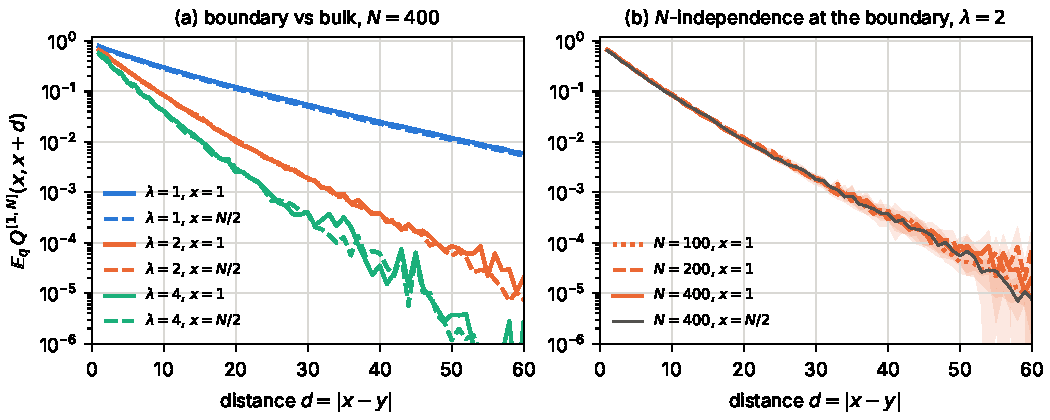
\includegraphics[width=\textwidth]{figs/correlator.pdf}
\caption{Sector-averaged eigenfunction correlator $\E_qQ^{[1,N]}_q(x,x+d)$ of
$\hq/J=-\Delta_N+\lambda\diag(q)$, over $4000$ i.i.d.\ samples of $q$ for each $(\lambda,N)$.  (a)
Boundary pairs $x=1$ (solid) and bulk pairs $x=N/2$ (dashed) at $N=400$ for $\lambda=1,2,4$.  The
boundary and bulk curves decay at the same rate, as Theorem~\ref{thm:EC} predicts.  (b) Boundary pairs
at $\lambda=2$ for $N=100,200,400$, with the bulk curve at $N=400$ (grey) and bands of $\pm2$ standard
errors: the boundary correlator does not depend on $N$.  Code:
\texttt{code/onebody\_correlator.py}; numerical values in \texttt{code/onebody\_correlator.out}.}
\label{fig:correlator}
\end{figure}

\begin{remark}[Numerical illustration]\label{rem:onebodynumerics}
\Cref{fig:correlator} shows $\E_qQ^{[1,N]}_q(x,x+d)$ for boundary and bulk pairs.  Least-squares fits of
$\log\E Q$ over $10\le d\le40$ give decay rates $\approx0.08$, $0.18$--$0.19$ and $0.21$--$0.23$ for
$\lambda=1,2,4$.  These values are the same, within the fluctuations of the fit, for boundary and bulk
pairs and for $N=100,200,400$; at $\lambda=4$ the estimates beyond $d\approx30$ are dominated by rare
samples.  The boundary values exceed the bulk values by a small but statistically significant amount at
$\lambda=1$: by $5$--$13\%$ for $1\le d\le40$ (e.g.\ $0.300$ versus $0.282$ at $d=10$, $N=400$).  The same
holds at $\lambda=2$ for $d=1$ only ($0.664$ versus $0.646$).  Otherwise the two agree within error.  For
comparison, the same code estimates $\gstar(\lambda)=\min_{E\in\Ilam}\gamma_\lambda(E)\approx0.13$, $0.34$,
$0.56$ for $\lambda=1,2,4$ (attained near $E=0$, $E\approx2.45$, $E\approx4.1$ respectively).  So the annealed
rate is well below $\gstar(\lambda)$, increasingly so as $\lambda$ grows, in line with \cref{rem:rate}(ii).
These numbers illustrate Theorem~\ref{thm:EC}; they are not used in any proof.
\end{remark}

% ============================================================================
% Section: Main results -- disorder-free localization
% ============================================================================
% Section-local macros (unique names, \providecommand only).
\providecommand{\cdr}{\tilde c}
\providecommand{\bent}{\mathsf{h}}           % binary entropy function (not the field h)
\providecommand{\Hsh}{\mathrm{H}}            % Shannon entropy
\providecommand{\Sfm}{S_{f}}                 % bare-matter entropy
\providecommand{\Ibar}{\bar I}
\providecommand{\rhoqf}[1]{\rho[#1]}         % quasi-free density matrix with symbol #1
\providecommand{\Alg}{\mathfrak{A}}
\providecommand{\BAlg}{\mathfrak{B}}
\providecommand{\GAlg}{\mathfrak{G}}
\providecommand{\SigF}{\Sigma_1(F)}
\providecommand{\SigpF}{\Sigma_1'(F)}
\providecommand{\ThF}{\Theta(F)}
\providecommand{\FZ}{F_{\Z}}
\providecommand{\Zone}{\one_N}

\section{Main results: disorder-free localization}\label{sec:main}

By the duality (\cref{thm:duality}) and the exact sector averaging (\cref{cor:sector}), every
expectation value of gauge-invariant observables (at any number of times) in the initial state
$\Psi_0=\ket{\uparrow\cdots\uparrow}_z\otimes\psi$ is an average over $2^N$ independent free-fermion
problems, one for each charge configuration $q$, with the i.i.d.\ Bernoulli one-body operators
$\hq=-J\Delta_N+2h\,\diag(q)$.  In this section we turn annealed one-body bounds into
statements about the gauge theory.

\emph{Status of the results.}  In finite volume all \emph{localization bounds} are stated under
Hypothesis~\ref{hyp:EC}, with explicit constants in terms of the moments $M_p(F)$, $M'_p(F)$ of
the function $F$ in \eqref{eq:hypEC}.  The structural results need no hypothesis: the lemmas of
\S\ref{sec:main:prelim} other than \cref{lem:annealed}, \cref{prop:LR}(a),(c),(d),
\cref{thm:imbalance}(i)--(iii), \cref{thm:arealaw}(a), \cref{prop:entropies}, \cref{lem:intentropy}
and the first bound of \cref{lem:duhamel}.
For every $\lambda=2h/J\neq0$, Theorem~\ref{thm:EC} proves Hypothesis~\ref{hyp:EC} with an exponential
function, $F(d)=\min\{1,Ce^{-\eta d}\}$.  So the finite-volume results hold unconditionally, but $C$ and $\eta$
are not explicit (\cref{rem:rate}).  The infinite-volume
statements (\cref{thm:infvol}) use only the Ge--Zhao bound on $\Z$ (\cref{prop:Zline}) and are
independent of Theorem~\ref{thm:EC}.  The constants are far from optimal; we state them because they
are explicit.  Two statements are conjectures (Conjectures~\ref{conj:logent} and~\ref{conj:volmix}).
Several arguments adapt methods developed for disordered XY chains
\cite{HSS2012,AbdulRahmanStolz2015,ANSS2016}, with the sector average in place of the average over a random
field; we say so where this applies (\cref{rem:main-transport,rem:main-LR,rem:main-arealaw}).

\emph{Overview.}
\Cref{thm:transport}: sector-averaged localization of the dressed-fermion propagator, bounded
moments and bounded transport across every cut.
\Cref{prop:LR}: a sector-averaged zero-velocity Lieb--Robinson bound, and the proof that no
operator-norm version exists.
\Cref{thm:imbalance}: a strictly positive infinite-time density-wave imbalance for every $h\neq0$,
uniformly in $N$.
\Cref{thm:arealaw,prop:entropies}: uniform-in-time area laws, and the precise relations between the
entropies $\SG,\Sfull,\Smix,\Sfm,\SN$.
\Cref{thm:numberentropy}: a uniform bound on the number entropy.
\Cref{thm:infvol}: thermodynamic limit.
\Cref{lem:duhamel} and Conjectures~\ref{conj:logent} and~\ref{conj:volmix}: what lies beyond.

\subsection{Preliminaries}\label{sec:main:prelim}

\paragraph{Standing notation.}
Throughout, $J>0$, $h\in\R\setminus\{0\}$ unless said otherwise, $N\ge2$, and $\E=\E_q$ is the
expectation over $q$ uniform on $\{\pm1\}^N$ (in finite volume a finite average, so no measurability
questions arise).  We write
\[
  U_q(t):=e^{-it\hq},\qquad Q_q:=Q^{[1,N]}_q,
\]
and $R_q$ for the time-averaged transition probability \eqref{eq:Rdef} of $\hq$.  Since $\hq$ is a
real symmetric matrix, $U_q(t)^{\top}=U_q(t)$, so $|U_q(t)_{xy}|=|U_q(t)_{yx}|$; and
$\sum_x|U_q(t)_{xy}|^2=1$.  The dressed fermions $\cdr_x$ are those of \eqref{eq:dressed}, and
$O(t):=e^{itH}Oe^{-itH}$ for operators $O$ on $\cH_N$.  For a Fock state $\psi=\ket{n}$ we write
$S:=\{x:n_x=1\}$ for its occupied set and
\begin{equation}\label{eq:main-K}
  K_q(t):=U_q(t)P_SU_q(t)^*,
\end{equation}
where $P_S$ is the orthogonal projection onto $\ell^2(S)$.  $K_q(t)$ is the projection onto
$U_q(t)\ell^2(S)$, and by \cref{cor:sector}(c),
$\langle\psi_q(t),c_x^\dagger c_y\psi_q(t)\rangle=\sum_{s\in S}\overline{U_q(t)_{xs}}U_q(t)_{ys}=K_q(t)_{yx}$.
The region $A$ consists of the sites $1,\dots,\ell$ and the links $b_1,\dots,b_\ell$ ($1\le\ell<N$), and
$\rho^q_A(t)$ denotes the reduced density matrix of $\psi_q(t)$ on the modes $1,\dots,\ell$, with the
identification of \S\ref{sec:model:cut}.  $\Hsh(p)=-\sum_kp(k)\ln p(k)$ is the Shannon entropy and
$\bent(\nu):=-\nu\ln\nu-(1-\nu)\ln(1-\nu)$ the binary entropy function (not to be confused with the
field $h$).

\paragraph{Constants.}  For $F$ as in Hypothesis~\ref{hyp:EC} we use
\begin{equation}\label{eq:main-constants}
\begin{gathered}
  \SigF:=\sum_{d\ge1}d\,F(d)\le M_1(F),\qquad
  \SigpF:=\sum_{d\ge1}d\,F(d)^{1/2}\le M'_1(F),\\
  \ThF:=2\sum_{k\ge1}k(2k+1)F(k)\le4M_2(F).
\end{gathered}
\end{equation}
The last inequality holds because $2k(2k+1)\le4(k+1)^2$.

\begin{lemma}[Sector-diagonal operators]\label{lem:sectornorm}
Let $X$ be a gauge-invariant operator on $\cH_N$.
\begin{enumerate}[label=(\alph*)]
\item $X=\sum_qP_qXP_q$ and $\norm{X}=\max_q\norm{P_qXP_q}$.
\item Let $\rho$ be a density matrix on $\cH_N$ and $w_q:=\Tr(\rho P_q)$ its sector weights.  Then
$|\Tr(\rho X)|\le\sum_qw_q\norm{P_qXP_q}$.  One has $w_q=2^{-N}$, and hence
$|\Tr(\rho X)|\le\E_q\norm{P_qXP_q}$, for $\rho=4^{-N}\one$ and for $\rho=\ket{\Psi_0}\bra{\Psi_0}$ with
$\Psi_0=\ket{\uparrow\cdots\uparrow}_z\otimes\psi$, where $\psi\in\cF_N$ is any unit vector.
\item If $X=\sum_qx_qP_q$ with $x_q\in\C$, then
$\langle\Psi_0,|X|\Psi_0\rangle=4^{-N}\Tr|X|=\E_q|x_q|$ for every $\Psi_0$ as in (b).
\end{enumerate}
\end{lemma}

\begin{proof}
(a) $X$ commutes with the orthogonal projections $P_q$, which sum to $\one$; the blocks $P_qXP_q$ act on
mutually orthogonal subspaces.  (b) By (a), $\Tr(\rho X)=\sum_q\Tr(P_q\rho P_q\,P_qXP_q)$, and
$|\Tr(\sigma Y)|\le\Tr(\sigma)\norm{Y}$ for $\sigma\ge0$.  The weights are $2^{-N}$ by
\cref{cor:sector}(a), resp.\ because $\Tr P_q=2^N$ (\cref{lem:gauss}(iii)).  (c) $|X|=\sum_q|x_q|P_q$; use
$\norm{P_q\Psi_0}^2=2^{-N}=4^{-N}\Tr P_q$.
\end{proof}

\paragraph{Quasi-free density matrices.}
\Cref{lem:quasifree,lem:slater} below are standard facts about quasi-free states.  We include short
proofs because we use them for arbitrary, also non-contiguous, sets of modes, with an explicit
identification of the tensor factors.
Let $A$ be a finite set of fermionic modes, $\cF_A$ the Fock space over $\ell^2(A)$, $c_x$ ($x\in A$) the
annihilation operators, $c(v):=\sum_x\overline{v(x)}c_x$, and $\Gamma(C)$ the second quantization of a
matrix $C$ on $\ell^2(A)$ ($\Gamma(C)\ket0=\ket0$,
$\Gamma(C)c^\dagger(u_1)\cdots c^\dagger(u_k)\ket0=c^\dagger(Cu_1)\cdots c^\dagger(Cu_k)\ket0$).  For
$0\le C\le\one$ with eigenvalues $\nu_1,\dots,\nu_{|A|}$ and an orthonormal eigenbasis $(v_i)$, put
$d_i:=c(v_i)$ and
\begin{equation}\label{eq:main-rhoC}
  \rhoqf{C}:=\prod_{i=1}^{|A|}\bigl(\nu_i\,d_i^\dagger d_i+(1-\nu_i)\,d_id_i^\dagger\bigr)
\end{equation}
(the factors commute).

\begin{lemma}[Quasi-free density matrices]\label{lem:quasifree}
Let $0\le C\le\one$ on $\ell^2(A)$.
\begin{enumerate}[label=(\alph*)]
\item With $N_A:=\sum_{x\in A}c_x^\dagger c_x$ and the convention that the $j=0$ term is $\Gamma(C)$,
\begin{equation}\label{eq:main-rhoformula}
  \rhoqf{C}=\sum_{j=0}^{|A|}\frac{(-1)^j}{j!}\sum_{x_1,\dots,x_j\in A}c_{x_1}\cdots c_{x_j}\,\Gamma(C)\,
  c^\dagger_{x_j}\cdots c^\dagger_{x_1}.
\end{equation}
In particular $\rhoqf{C}$ does not depend on the choice of eigenbasis, its matrix elements in the
occupation basis are polynomials in the entries of $C$, and $C\mapsto\rhoqf{C}$ is uniformly continuous
on $\{0\le C\le\one\}$.
\item $\rhoqf{C}$ is a density matrix with $S(\rhoqf{C})=\sum_i\bent(\nu_i)$.  Under $\rhoqf{C}$, $N_A$ has
the law of $\sum_i\xi_i$ with independent $\xi_i\sim\mathrm{Bernoulli}(\nu_i)$; its generating function is
$\Tr(\rhoqf{C}z^{N_A})=\det(\one+(z-1)C)$, and its variance is $\Tr(C-C^2)$.
\end{enumerate}
\end{lemma}

\begin{proof}
(a) For every operator $Y$ on $\cF_A$,
$\sum_id_iYd_i^\dagger=\sum_{x,y}\bigl(\sum_i\overline{v_i(x)}v_i(y)\bigr)c_xYc_y^\dagger=\sum_xc_xYc_x^\dagger$,
by completeness of $(v_i)$.  Iterating, the inner sum in \eqref{eq:main-rhoformula} equals
$\Xi_j:=\sum_{i_1,\dots,i_j}d_{i_1}\cdots d_{i_j}\Gamma(C)d^\dagger_{i_j}\cdots d^\dagger_{i_1}$.  Let
$\ket{T}:=\prod_{i\in T}d_i^\dagger\ket0$ (increasing order) for $T\subset\{1,\dots,|A|\}$.  The vector
$\phi:=d^\dagger_{i_j}\cdots d^\dagger_{i_1}\ket T$ vanishes unless $i_1,\dots,i_j$ are distinct and not in
$T$; then $\phi=\pm\ket{T\cup R}$ with $R=\{i_1,\dots,i_j\}$, $\Gamma(C)\phi=\prod_{i\in T\cup R}\nu_i\,\phi$
because $Cv_i=\nu_iv_i$, and $d_{i_1}\cdots d_{i_j}\phi=\ket T$.  Each set $R$ arises from $j!$ ordered
tuples, so
\[
  \sum_j\frac{(-1)^j}{j!}\Xi_j\ket T=\sum_{R\subset T^c}(-1)^{|R|}\prod_{i\in T\cup R}\nu_i\,\ket T
  =\prod_{i\in T}\nu_i\prod_{i\notin T}(1-\nu_i)\,\ket T=\rhoqf{C}\ket T .
\]
The right side of \eqref{eq:main-rhoformula} involves only $C$, and the matrix elements of $\Gamma(C)$ in
the occupation basis are minors of $C$.  A continuous function on a compact set is uniformly continuous.

(b) In the basis $(\ket T)$, $\rhoqf{C}$ is diagonal with eigenvalues
$w_T=\prod_{i\in T}\nu_i\prod_{i\notin T}(1-\nu_i)\ge0$, the law of independent Bernoulli$(\nu_i)$
variables, and $N_A=\sum_id_i^\dagger d_i$ (completeness again) acts on $\ket T$ as $|T|$.  The entropy of a
product law is the sum of the entropies of its factors.  Finally
$\sum_Tw_Tz^{|T|}=\prod_i(1-\nu_i+z\nu_i)=\det(\one+(z-1)C)$, and
$\Var\sum_i\xi_i=\sum_i\nu_i(1-\nu_i)$.
\end{proof}

\begin{lemma}[Reduced states of Slater determinants]\label{lem:slater}
Let $\Lambda$ be a finite set of modes, $W\subset\ell^2(\Lambda)$ a subspace of dimension $M$ with orthogonal
projection $K$, and $\psi_W:=c^\dagger(w_1)\cdots c^\dagger(w_M)\ket0$ for an orthonormal basis $(w_j)$ of $W$
(unique up to a phase).  Let $A\subset\Lambda$, $B:=\Lambda\setminus A$, and identify
$\cF_\Lambda\cong\cF_A\otimes\cF_B$ by $c(a)\mapsto c(a)\otimes\one$, $c(b)\mapsto(-1)^{N_A}\otimes c(b)$ for
$a\in\ell^2(A)$, $b\in\ell^2(B)$, $\ket0\mapsto\ket0\otimes\ket0$.  (For $A=\{1,\dots,\ell\}$ this is the
identification of \S\ref{sec:model:cut}.)  Under it, the CAR algebra of the modes in $A$ is
$\mathcal B(\cF_A)\otimes\one$, and we let $\rho_A:=\Tr_{\cF_B}\ket{\psi_W}\bra{\psi_W}$.  Let
$C_A:=P_AKP_A$, regarded as an operator on $\ell^2(A)$, with eigenvalues $\nu_1,\dots,\nu_{|A|}$, and
$T:=P_BKP_A$.  Then:
\begin{enumerate}[label=(\alph*)]
\item $\rho_A=\rhoqf{C_A}$.  Hence $S(\rho_A)=\sum_i\bent(\nu_i)$, and the law of $N_A$ under $\psi_W$ is the
Poisson-binomial law of \cref{lem:quasifree}(b).
\item $C_A-C_A^2=T^*T$.  Hence
$\Var_{\psi_W}(N_A)=\norm{T}_2^2=\sum_{x\in A,\,y\in B}|K_{yx}|^2$ and
$\sum_i\sqrt{\nu_i(1-\nu_i)}=\norm{T}_1\le\sum_{x\in A,\,y\in B}|K_{yx}|$.
\end{enumerate}
\end{lemma}

\begin{proof}
(a) Changing the basis of $W$ multiplies $\psi_W$ by a determinant of modulus one, so we may take $w_j$ to be
an orthonormal eigenbasis of $W$ for the operator $(P_A|_W)^*(P_A|_W)$, with eigenvalues
$\mu_j\in[0,1]$.  Then $\langle P_Aw_j,P_Aw_k\rangle=\mu_j\delta_{jk}$ and
$\langle P_Bw_j,P_Bw_k\rangle=(1-\mu_j)\delta_{jk}$.  Put $a_j:=\mu_j^{-1/2}P_Aw_j$ if $\mu_j>0$ and
$b_j:=(1-\mu_j)^{-1/2}P_Bw_j$ if $\mu_j<1$; these are orthonormal families in $\ell^2(A)$, resp.\ $\ell^2(B)$,
and $w_j=\sqrt{\mu_j}\,a_j+\sqrt{1-\mu_j}\,b_j$ (a term with vanishing coefficient is absent).  Expanding
the product $\prod_jc^\dagger(w_j)$ and moving all $c^\dagger(a_j)$ to the left,
\[
  \psi_W=\sum_{T\subset\{1,\dots,M\}}\varepsilon_T\prod_{j\in T}\sqrt{\mu_j}\prod_{j\notin T}\sqrt{1-\mu_j}\;
  c^\dagger(a_T)\,c^\dagger(b_{T^c})\ket0,
\]
with signs $\varepsilon_T=\pm1$ and $c^\dagger(a_T):=\prod_{j\in T}c^\dagger(a_j)$ in increasing order.  Under the
identification, $c^\dagger(a_T)c^\dagger(b_{T^c})\ket0\mapsto\alpha_T\otimes\beta_{T^c}$ with
$\alpha_T:=c^\dagger(a_T)\ket0$, $\beta_{T^c}:=c^\dagger(b_{T^c})\ket0$, because the factors $(-1)^{N_A}$ act on the
vacuum of $\cF_A$.  The $\alpha_T$ with nonzero coefficient are orthonormal, and so are the $\beta_{T^c}$.  Hence
this is a Schmidt decomposition, and
$\rho_A=\sum_T\prod_{j\in T}\mu_j\prod_{j\notin T}(1-\mu_j)\,\ket{\alpha_T}\bra{\alpha_T}$.  On the other hand
$C_A=\sum_j\ket{P_Aw_j}\bra{P_Aw_j}=\sum_{j:\mu_j>0}\mu_j\ket{a_j}\bra{a_j}$, so $C_A$ has the eigenvectors
$a_j$ ($\mu_j>0$) with eigenvalues $\mu_j$, and eigenvalue $0$ on the orthogonal complement in $\ell^2(A)$.
Computing \eqref{eq:main-rhoC} in this eigenbasis gives the same operator.  The rest is
\cref{lem:quasifree}(b); $N_A\otimes\one$ belongs to the algebra of $A$.

(b) Since $K=K^*=K^2$, $C_A-C_A^2=P_AK(\one-P_A)KP_A=T^*T$.  So
$\sum_i\nu_i(1-\nu_i)=\Tr T^*T=\norm{T}_2^2$ and $\sum_i\sqrt{\nu_i(1-\nu_i)}=\Tr|T|=\norm T_1$.  Finally
$T=\sum_{x\in A,y\in B}K_{yx}\ket{\delta_y}\bra{\delta_x}$ is a sum of rank-one operators of trace norm
$|K_{yx}|$.
\end{proof}

\begin{lemma}[Binary entropy]\label{lem:binent}
For all $\nu\in[0,1]$: $\bent(\nu)\le2\ln2\,\sqrt{\nu(1-\nu)}$, with equality iff $\nu\in\{0,\tfrac12,1\}$.
\end{lemma}

\begin{proof}
Both sides vanish at $\nu\in\{0,1\}$ and are symmetric under $\nu\mapsto1-\nu$.  Write $\nu=(1-s)/2$ with
$s\in[0,1)$.  The function $f(s):=(1+s)\ln(1+s)+(1-s)\ln(1-s)$ satisfies $f(0)=f'(0)=0$ and
$f''(s)=2/(1-s^2)=2\sum_{j\ge0}s^{2j}$, hence $f(s)=\sum_{k\ge1}s^{2k}/(k(2k-1))$ and
\[
  \bent(\nu)=\ln2-\tfrac12f(s)=\ln2-\sum_{k\ge1}e_ks^{2k},\qquad e_k:=\frac1{2k(2k-1)} .
\]
Moreover $2\ln2\sqrt{\nu(1-\nu)}=\ln2\sqrt{1-s^2}=\ln2\,\bigl(1-\sum_{k\ge1}c_ks^{2k}\bigr)$ with
$c_k:=\binom{2k}{k}\frac1{(2k-1)4^k}>0$.  So the claim is $\sum_{k\ge1}d_ks^{2k}\ge0$ with
$d_k:=e_k-c_k\ln2$.  We have $d_1=\frac12(1-\ln2)>0$.  The ratio
$e_k/c_k=4^k/\bigl(2k\binom{2k}{k}\bigr)$ satisfies $(e_{k+1}/c_{k+1})/(e_k/c_k)=2k/(2k+1)<1$, and
$e_2/c_2=\frac23<\ln2$; hence $d_k<0$ for all $k\ge2$.  Letting $s\uparrow1$ (monotone convergence; all
$e_k,c_k>0$) gives $\sum_ke_k=\frac12f(1)=\ln2$ and $\sum_kc_k=1$, so $\sum_{k\ge2}d_k=-d_1$.  Since
$s^{2k}\le s^4$ for $k\ge2$,
\[
  \sum_{k\ge1}d_ks^{2k}\ge d_1s^2+s^4\sum_{k\ge2}d_k=d_1(s^2-s^4)\ge0,
\]
with equality for $s\in[0,1)$ only if $s=0$, i.e.\ $\nu=\frac12$.
\end{proof}

\begin{lemma}[Annealed one-body bounds]\label{lem:annealed}
Assume Hypothesis~\ref{hyp:EC}.  Let $\psi$ be a Fock state with occupied set $S$ (arbitrary), and
$x\neq y$ in $[1,N]$, $d:=|x-y|$.
\begin{enumerate}[label=(\roman*)]
\item $\displaystyle\E\sup_{t\in\R}|K_q(t)_{xy}|\le\E\sum_{z=1}^NQ_q(x,z)Q_q(y,z)\le2\sum_{k\ge\lceil d/2\rceil}F(k)$.
\item For $1\le m<N$:
\begin{gather*}
  \E\sup_t\sum_{x\le m<y}|K_q(t)_{xy}|\le\ThF,\qquad
  \E\sum_{x\le m<z}Q_q(x,z)\le\SigF,\\
  \E\Bigl(\sum_{x\le m<z}Q_q(x,z)\Bigr)^2\le\SigpF^2 .
\end{gather*}
\item For an interval $B\subset[1,N]$ the same bounds hold for the sums over pairs $x\in B$,
$y\in[1,N]\setminus B$, with the constants $2\ThF$, $2\SigF$ and $4\SigpF^2$.
\end{enumerate}
\end{lemma}

\begin{proof}
(i) $|K_q(t)_{xy}|\le\sum_{s\in S}|U_q(t)_{xs}||U_q(t)_{ys}|\le\sum_z Q_q(x,z)Q_q(y,z)$ for all $t$, by
\cref{lem:consequences}(b).  By \eqref{eq:cons2},
$\E[Q_q(x,z)Q_q(y,z)]\le F(\max\{|x-z|,|y-z|\})$.  Let $x<y$.  For $z\in[x,y]$ the value
$k=\max\{z-x,y-z\}$ lies in $[\lceil d/2\rceil,d]$, and each such $k$ arises for at most two $z$; for $z<x$
or $z>y$ it equals $d+|z-x|$, resp.\ $d+|z-y|$, so each $k>d$ arises at most twice.  Hence the sum is at
most $2\sum_{k\ge\lceil d/2\rceil}F(k)$.

(ii) The number of pairs $x\le m<y$ with $y-x=d$ is at most $d$.  By (i),
\[
  \E\sup_t\sum_{x\le m<y}|K_q(t)_{xy}|\le\sum_{d\ge1}d\cdot2\sum_{k\ge\lceil d/2\rceil}F(k)
  =2\sum_{k\ge1}F(k)\sum_{d=1}^{2k}d=2\sum_{k\ge1}k(2k+1)F(k).
\]
The second bound is \eqref{eq:hypEC} with the same counting.  For the third, by \eqref{eq:cons3},
$\E(\sum_iQ_i)^2=\sum_{i,j}\E Q_iQ_j\le(\sum_iF(d_i)^{1/2})^2\le\SigpF^2$, where $i$ runs over the pairs
and $d_i$ is the distance of pair $i$.

(iii) The number of pairs $x\in B$, $y\notin B$ at distance $d$ is at most $2d$.
\end{proof}

\begin{lemma}[Finite propagation speed]\label{lem:propagation}
Let $\Lambda\subset\Lambda'\subset\Z$ be intervals ($\Lambda'=\Z$ allowed), $v:\Lambda'\to\R$ with $|v|\le V_0$,
$k_{\Lambda}:=-J\Delta_\Lambda+\diag(v|_\Lambda)$ on $\ell^2(\Lambda)$, likewise $k_{\Lambda'}$, and $c:=|t|(2J+V_0)$.  For
$x,y\in\Lambda$:
\begin{enumerate}[label=(\alph*)]
\item $|(e^{-itk_\Lambda})_{xy}|\le e^{c}\,c^{|x-y|}/|x-y|!$;
\item $|(e^{-itk_\Lambda})_{xy}-(e^{-itk_{\Lambda'}})_{xy}|\le2e^{c}\,c^{n_0}/n_0!$, where
$n_0:=\dist(x,\Lambda'\setminus\Lambda)+\dist(y,\Lambda'\setminus\Lambda)$ (the left side is $0$ if $\Lambda=\Lambda'$).
\end{enumerate}
\end{lemma}

\begin{proof}
$\norm{k_\Lambda},\norm{k_{\Lambda'}}\le2J+V_0$, and $e^{-itk}=\sum_n(-it)^nk^n/n!$ converges in norm.  The
entry $(k^n)_{xy}$ is a sum over paths $x=z_0,z_1,\dots,z_n=y$ with $|z_{i+1}-z_i|\le1$ of products of matrix
entries.  (a) $(k_\Lambda^n)_{xy}=0$ for $n<|x-y|$ and $|(k^n_\Lambda)_{xy}|\le\norm{k_\Lambda}^n$, so the entry is at
most $\sum_{n\ge d}c^n/n!\le e^cc^d/d!$ with $d=|x-y|$.  (b) A path from $x$ to $y$ that visits
$\Lambda'\setminus\Lambda$ has length at least $n_0$, and on paths inside $\Lambda$ the entries of $k_\Lambda$ and
$k_{\Lambda'}$ agree.  So $(k_\Lambda^n)_{xy}=(k^n_{\Lambda'})_{xy}$ for $n<n_0$, and the difference is at most
$2\sum_{n\ge n_0}c^n/n!\le2e^cc^{n_0}/n_0!$.
\end{proof}

\subsection{Localization of dressed fermions and bounded transport}\label{sec:main:transport}

\begin{theorem}[Dressed-fermion localization and bounded transport]\label{thm:transport}
Assume Hypothesis~\ref{hyp:EC}, and let $\Psi_0=\ket{\uparrow\cdots\uparrow}_z\otimes\psi$,
$\Psi(t)=e^{-itH}\Psi_0$.  For all $N\ge2$:
\begin{enumerate}[label=(\alph*)]
\item \emph{(Propagator.)}  For all $x,y\in[1,N]$ and $t\in\R$,
\begin{equation}\label{eq:main-anticomm}
  \{\cdr_x(t),\cdr_y^\dagger\}=\sum_qU_q(t)_{xy}\,P_q .
\end{equation}
Thus the dressed-fermion propagator is the scalar $U_q(t)_{xy}$ in each sector, and its sector-averaged
modulus is localized uniformly in time:
\begin{equation}\label{eq:main-prop}
  \E_q\sup_{t\in\R}\norm{P_q\{\cdr_x(t),\cdr_y^\dagger\}P_q}=\E_q\sup_{t\in\R}|U_q(t)_{xy}|\le F(|x-y|).
\end{equation}
In particular, $\sup_t\langle\Psi_0,|\{\cdr_x(t),\cdr_y^\dagger\}|\,\Psi_0\rangle\le F(|x-y|)$ for every
matter state $\psi$.
\item \emph{(One particle: moments.)}  If $\psi=f_y^\dagger\ket0$, then for $0\le p\le2$,
\[
  \sup_{t\in\R}\sum_{x=1}^N(|x-y|+1)^p\langle\Psi(t),n_x\Psi(t)\rangle
  \le\E_q\sup_{t\in\R}\sum_{x=1}^N(|x-y|+1)^p|U_q(t)_{xy}|^2\le2M_p(F).
\]
\item \emph{(Transport across any cut.)}  Let $\psi=\ket n$ be a Fock state with occupied set $S$, let
$1\le m<N$ and $s_m:=|S\cap[1,m]|$.  Then for every $q$ and $t$,
$|\langle\psi_q(t),N_{\le m}\psi_q(t)\rangle-s_m|\le\sum_{x\le m<z}|U_q(t)_{xz}|^2$, and
\begin{gather}
  \E_q\sup_t\bigl|\langle\psi_q(t),N_{\le m}\psi_q(t)\rangle-s_m\bigr|\le\SigF\le M_1(F),\qquad
  \sup_t\bigl|\langle\Psi(t),N_{\le m}\Psi(t)\rangle-s_m\bigr|\le\SigF,\label{eq:main-transport}\\
  \sup_t\bigl\langle\Psi(t),(N_{\le m}-s_m)^2\Psi(t)\bigr\rangle\le\ThF+\SigpF^2\le4M_2(F)+M'_1(F)^2.
  \label{eq:main-transport2}
\end{gather}
In particular $\Prob_{\Psi(t)}(|N_{\le m}-s_m|\ge k)\le(4M_2(F)+M'_1(F)^2)/k^2$ for all $t$ and $k>0$.
\item \emph{(Dressed correlations.)}  For Fock $\psi$ and $x\neq y$,
$\sup_t|\langle\Psi(t),\cdr_x^\dagger\cdr_y\Psi(t)\rangle|\le2\sum_{k\ge\lceil|x-y|/2\rceil}F(k)$; here
$\cdr_x^\dagger\cdr_y=f_x^\dagger(\prod_{x\le k<y}\sigma^z_{b_k})f_y$ for $x<y$ (\cref{thm:duality}(d)).
\end{enumerate}
All bounds are uniform in $N$, in the position of the cut and in $t$.
\end{theorem}

\begin{proof}
(a) By \eqref{eq:heisenberg}, $\cdr_x(t)=\sum_qP_q\sum_zU_q(t)_{xz}\cdr_z$.  The $\cdr$'s commute with every
$G_k$ (\cref{thm:duality}(d)), hence with $P_q$, and satisfy the CAR.  So
$\{\cdr_x(t),\cdr_y^\dagger\}=\sum_qP_q\sum_zU_q(t)_{xz}\delta_{zy}$, which is \eqref{eq:main-anticomm}.
Then $P_q\{\cdr_x(t),\cdr_y^\dagger\}P_q=U_q(t)_{xy}P_q$ with $P_q\neq0$, which gives the identity in
\eqref{eq:main-prop}; the bound is \eqref{eq:cons1}.  The last statement is \cref{lem:sectornorm}(c), together with
$\E_q|U_q(t)_{xy}|\le\E_q\sup_s|U_q(s)_{xy}|$.

(b) Here $\psi_q(t)=c^\dagger(U_q(t)\delta_y)\ket0$, so that
$\langle\psi_q(t),n_x\psi_q(t)\rangle=|U_q(t)_{xy}|^2$, and
$\langle\Psi(t),n_x\Psi(t)\rangle=\E_q|U_q(t)_{xy}|^2$ by \cref{cor:sector}(b),(c).  Exchange the finite sums,
use $\sup_t\E\le\E\sup_t$, and apply \eqref{eq:cons4}.

(c) By \cref{cor:sector}(c), $\langle\psi_q(t),n_x\psi_q(t)\rangle=\sum_{s\in S}|U_q(t)_{xs}|^2$.  Using
$\sum_{x=1}^N|U_q(t)_{xs}|^2=1$ for the $s\in S\cap[1,m]$,
\[
  \langle\psi_q(t),N_{\le m}\psi_q(t)\rangle-s_m=\sum_{x\le m,\ s\in S,\ s>m}|U_q(t)_{xs}|^2-\sum_{x>m,\ s\in S,\ s\le m}|U_q(t)_{xs}|^2 .
\]
Both sums are non-negative.  Since $|U_q(t)_{xs}|=|U_q(t)_{sx}|$, both are at most
\[
  D_q(t):=\sum_{x\le m<z}|U_q(t)_{xz}|^2,
\]
and the difference of two numbers in $[0,D]$ has modulus at most $D$.  Next, $D_q(t)\le Y_q:=\sum_{x\le m<z}Q_q(x,z)$, and $\E Y_q\le\SigF$ by \cref{lem:annealed}(ii).  The
LGT statement follows from \cref{cor:sector}(b), which gives
\[
  \langle\Psi(t),N_{\le m}\Psi(t)\rangle=\E_q\langle\psi_q(t),N_{\le m}\psi_q(t)\rangle .
\]
For \eqref{eq:main-transport2}: by \cref{cor:sector}(c) the law of $N_{\le m}$ in $\Psi(t)$ is the $q$-average of its
laws in the $\psi_q(t)$.  Hence
\[
  \langle\Psi(t),(N_{\le m}-s_m)^2\Psi(t)\rangle=\E_q\bigl[\Var_q(t)+(\langle\psi_q(t),N_{\le m}\psi_q(t)\rangle-s_m)^2\bigr],
\]
where $\Var_q(t)$ is the variance of $N_{\le m}$ in $\psi_q(t)$.  By \cref{lem:slater}(b) with $A=[1,m]$,
$\Var_q(t)=\sum_{x\le m<y}|K_q(t)_{xy}|^2\le\sum_{x\le m<y}|K_q(t)_{xy}|$, whose $\E\sup_t$ is at most $\ThF$ by
\cref{lem:annealed}(ii).  The second term is at most $\E Y_q^2\le\SigpF^2$.  The probability bound is
Chebyshev's inequality.

(d) $\langle\Psi(t),\cdr_x^\dagger\cdr_y\Psi(t)\rangle=\E_qK_q(t)_{yx}$ by \cref{cor:sector}(b),(c); apply
\cref{lem:annealed}(i).
\end{proof}

\begin{remark}[On the statement]\label{rem:main-transport}
(i) The supremum over $t$ is \emph{inside} the sector average, which is stronger than a bound on
$\sup_t\E_q$: in a typical sector the dressed fermion stays localized for all times.
(ii) By \cref{lem:productlaw}(c), \cref{thm:transport} holds verbatim for every $\sigma^z$-product gauge
state $\ket{s}_z$ in place of $\ket{\uparrow\cdots\uparrow}_z$.  For any gauge state whose sector law
has density at most $K$ with respect to the uniform law (e.g.\ $K=2$ for the open chain,
\cref{prop:variants}(i)), all bounds of \cref{thm:transport} hold with an extra factor $K$ (for Fock $\psi$ every
sector carries $\ket n$ up to a phase, by \cref{lem:productlaw}(b)).  This uses that they are upper bounds on
averages of non-negative sector functionals (\cref{rem:productlaws}(c)); lower bounds, such as
\cref{thm:imbalance}, do not transfer in this way.  For the dimer law of \cref{lem:productlaw}(e) and
$0<2|h|<J$, the moment bound (b) fails uniformly in $N$, and so does the analogue of
Hypothesis~\ref{hyp:EC} (\cref{thm:dimer}(d)).
(iii) Hypothesis~\ref{hyp:EC} enters only through \eqref{eq:hypEC} and its consequences
\eqref{eq:cons1}--\eqref{eq:cons4}:
(a) uses \eqref{eq:cons1}, (b) uses \eqref{eq:cons4}, (c) uses \eqref{eq:hypEC} itself together with
\eqref{eq:cons2} and \eqref{eq:cons3}, and (d) uses \eqref{eq:cons2}.  Part (c) is the gauge-theory analogue
of the disorder-averaged particle-transport bound for disordered XX chains in
\cite[Thm.~1.1]{ANSS2016}.
(iv) \emph{Numerical check} (\texttt{code/main\_checks.py}, part A; $N=60$, $\lambda=2$, CDW, $300$
sectors, $62$ times in $[0,10^5]$): the deterministic inequalities in the proof of (c) and the moment
inequalities hold to $4\times10^{-14}$, and $U_q(t)^\top=U_q(t)$ to $3\times10^{-16}$.  The measured
$\E\sup_t$ of the transported charge across the middle cut is $0.52$.  The bound $\SigF$ evaluated with
the empirical correlator $F_{\rm emp}$ (the non-increasing envelope of $\max_x\E Q_q(x,x+d)$, an
estimate, not a proof) is $20$.  For one particle, $\E\sup_t\sum_x(|x-y|+1)^2|U_q(t)_{xy}|^2=33$,
against $2M_2(F_{\rm emp})\approx5\times10^2$.
\end{remark}

\subsection{A sector-averaged zero-velocity Lieb--Robinson bound}\label{sec:main:LR}

For $X\subset[1,N]$ let $\Alg(X)$ be the $*$-algebra generated by $\{\cdr_x:x\in X\}$ and $\Alg^+(X)$ its even
part (spanned by monomials of even degree).  For $Y\subset[1,N]$ let $\BAlg^+(Y)$ be the $*$-algebra generated by
$\Alg^+(Y)$ and $G_1,\dots,G_N$.  All these operators are gauge invariant.  The generators of $\Alg^+(X)$ are local
in the original variables: for $x<y$, $\cdr_x^\dagger\cdr_y=f_x^\dagger(\prod_{x\le k<y}\sigma^z_{b_k})f_y$ and
$\cdr_x\cdr_y=f_xf_y\prod_{x\le k<y}\sigma^z_{b_k}$, and $\cdr_x^\dagger\cdr_x=n_x$ (\cref{thm:duality}(d)).
$\BAlg^+(Y)$ also contains the electric energies $\sigma^x_{b_{j-1}}\sigma^x_{b_j}=G_j(-1)^{n_j}$, $j\in Y$.  The
operators $\gamma_{2x-1}:=\cdr_x+\cdr_x^\dagger$ and $\gamma_{2x}:=i(\cdr_x^\dagger-\cdr_x)$, $x\in X$, are self-adjoint
unitaries.  For an ordered set $\mathcal S$ of indices let $\gamma_{\mathcal S}$ be the ordered product.  Every
$A\in\Alg(X)$ has a unique expansion $A=\sum_{\mathcal S}a_{\mathcal S}\gamma_{\mathcal S}$ (see the proof), and we
put $|A|_1:=\sum_{\mathcal S}|a_{\mathcal S}|\le4^{|X|}\norm{A}$.

\begin{proposition}[Sector-averaged zero-velocity Lieb--Robinson bound]\label{prop:LR}
Let $X,Y\subset[1,N]$ and $B\in\BAlg^+(Y)$.
\begin{enumerate}[label=(\alph*)]
\item \emph{(Sector-wise bound; no hypothesis.)}  For a monomial $A=\cdr^{\sharp}_{x_1}\cdots\cdr^{\sharp}_{x_k}$
($x_i\in X$, each $\cdr^\sharp$ equal to $\cdr$ or $\cdr^\dagger$), and for every $q$ and $t$,
\begin{equation}\label{eq:main-LRsector}
  \norm{P_q[A(t),B]}\le2\norm B\sum_{i=1}^k\sum_{y\in Y}|U_q(t)_{x_iy}| .
\end{equation}
For general $A\in\Alg(X)$, $\norm{P_q[A(t),B]}\le8|A|_1\norm B\sum_{x\in X,y\in Y}|U_q(t)_{xy}|$.
\item \emph{(Sector-averaged zero-velocity bound.)}  Under Hypothesis~\ref{hyp:EC},
\begin{equation}\label{eq:main-LR}
\begin{gathered}
  \E_q\sup_{t\in\R}\norm{P_q[A(t),B]P_q}\le2\norm B\sum_{i=1}^k\sum_{y\in Y}F(|x_i-y|),\\
  \text{resp.}\quad\E_q\sup_{t\in\R}\norm{P_q[A(t),B]P_q}\le8|A|_1\norm B\sum_{x\in X,y\in Y}F(|x-y|).
\end{gathered}
\end{equation}
Consequently, let $\rho$ be a density matrix whose sector weights satisfy $\Tr(\rho P_q)\le K2^{-N}$ for all
$q$.  Then $\sup_t|\Tr(\rho[A(t),B])|$ is at most $K$ times the right side of \eqref{eq:main-LR}.  This covers $K=1$ and
$\rho=\ket{\Psi_0}\bra{\Psi_0}$, $\Psi_0=\ket{\uparrow\cdots\uparrow}_z\otimes\psi$, with \emph{arbitrary} $\psi$, as well
as $\rho=4^{-N}\one$.
\item \emph{(The operator norm sees the clean sector.)}  For all $N$, $x,y\in[1,N]$ and $t$,
\begin{equation}\label{eq:main-LRnorm}
\begin{gathered}
  \norm{\{\cdr_x(t),\cdr_y^\dagger\}}=\norm{[\cdr_x(t),n_y]}=\max_q|U_q(t)_{xy}|,\\
  \norm{[n_x(t),n_y]}=\max_q|U_q(t)_{xy}|\bigl(1-|U_q(t)_{xy}|^2\bigr)^{1/2}.
\end{gathered}
\end{equation}
The maximum includes the clean sector $q=\Zone=(1,\dots,1)$.  It has probability $2^{-N}$ under the sector
law, which vanishes as $N\to\infty$.  In particular, for $N\ge2$,
\[
  \sup_t\norm{\{\cdr_1(t),\cdr_N^\dagger\}}\ge\Bigl(\frac{3}{2(N+1)}\Bigr)^{1/2},\qquad
  \sup_t\norm{[n_1(t),n_N]}\ge\Bigl(\frac{3}{4(N+1)}\Bigr)^{1/2},
\]
whereas the sector average in \eqref{eq:main-prop} is at most $F(N-1)$.
\item \emph{(No operator-norm zero-velocity bound.)}  There is no function $G:\N_0\to[0,\infty)$ such that
$\sum_dd^2G(d)^2<\infty$ and $\sup_t\norm{[n_x(t),n_y]}\le G(|x-y|)$ for all $N\ge1$ and all $x,y\in[1,N]$.
The same holds with $[n_x(t),n_y]$ replaced by $\{\cdr_x(t),\cdr_y^\dagger\}$ or by $[\cdr_x(t),n_y]$.
\end{enumerate}
\end{proposition}

\begin{proof}
(a) All operators involved are gauge invariant, so they commute with $P_q$.  Replacing each $G_j$ in $B$ by
$q_j$ gives $B_q\in\Alg^+(Y)$ with $P_qB=P_qB_q$.  If $z\notin Y$, then $\cdr_z$ anticommutes with $\cdr_y$ and
$\cdr_y^\dagger$ for all $y\in Y$, hence commutes with every even monomial, and $[\cdr_z,B_q]=0$.  By
\eqref{eq:heisenberg},
\[
  P_q[\cdr_x(t),B]=\sum_{z}U_q(t)_{xz}P_q[\cdr_z,B_q]=\sum_{y\in Y}U_q(t)_{xy}P_q[\cdr_y,B_q],
\]
and $\norm{P_q[\cdr_y,B_q]}\le\norm{\cdr_yP_qB_q}+\norm{P_qB_q\cdr_y}\le2\norm{P_qB}\le2\norm B$, because $P_q$
commutes with $\cdr_y$.  The same holds for $\cdr_x(t)^\dagger$, with $\overline{U_q(t)_{xy}}$.  For a monomial,
$[a_1\cdots a_k,B]=\sum_ia_1\cdots a_{i-1}[a_i,B]a_{i+1}\cdots a_k$.  Moving $P_q$ through
$a_1(t),\dots,a_{i-1}(t)$, which have norm one, gives \eqref{eq:main-LRsector}.

For general $A$ we first justify the expansion.  The products $\gamma_{\mathcal S}$, with $\mathcal S$ ranging over
the subsets of the $2|X|$ indices in increasing order, span $\Alg(X)$, since $\gamma_j^2=\one$ and distinct
$\gamma$'s anticommute.  Let $\tau:=4^{-N}\Tr$.  If $\mathcal S\neq\emptyset$, then $\tau(\gamma_{\mathcal S})=0$.
Indeed, for $|\mathcal S|$ odd, $\gamma_{\mathcal S}$ anticommutes with $(-1)^{N_f}$, since the $\cdr$'s are odd.  For
$|\mathcal S|$ even and $j\in\mathcal S$, $\gamma_j\gamma_{\mathcal S}\gamma_j=-\gamma_{\mathcal S}$.  In both cases
cyclicity of the trace gives $\tau(\gamma_{\mathcal S})=-\tau(\gamma_{\mathcal S})$.  Since
$\gamma_{\mathcal S}^*\gamma_{\mathcal S'}=\pm\gamma_{\mathcal S\triangle\mathcal S'}$, the $\gamma_{\mathcal S}$ are orthonormal for
$(A_1,A_2)\mapsto\tau(A_1^*A_2)$, the expansion is unique, and $a_{\mathcal S}=\tau(\gamma_{\mathcal S}^*A)$, so
$|a_{\mathcal S}|\le\norm A$.  As above,
$\norm{P_q[\gamma_{2x-1}(t),B]},\norm{P_q[\gamma_{2x}(t),B]}\le4\norm B\sum_{y\in Y}|U_q(t)_{xy}|$, and each
$x\in X$ carries two indices.  So
$\norm{P_q[\gamma_{\mathcal S}(t),B]}\le8\norm B\sum_{x\in X,y\in Y}|U_q(t)_{xy}|$.  Sum over $\mathcal S$.

(b) Take $\sup_t$ and $\E_q$ in (a) and use \eqref{eq:cons1}.  The statement on states is
\cref{lem:sectornorm}(b) applied to the gauge-invariant operator $X=[A(t),B]$.

(c) The first norm is $\max_q|U_q(t)_{xy}|$ by \eqref{eq:main-anticomm} and \cref{lem:sectornorm}(a).  Since
$[\cdr_z,\cdr_y^\dagger\cdr_y]=\delta_{zy}\cdr_y$, the computation in (a) gives
$P_q[\cdr_x(t),n_y]=U_q(t)_{xy}P_q\cdr_y$.  In the dual picture $P_q\cdr_y$ is $c_y\otimes\ket q\bra q$, of norm one.
For $[n_x(t),n_y]$ we use the dual picture in the sector $q$.  With $u:=U_q(t)$ and $w:=u^*\delta_x$, we have
$\Gamma(u)^*\dGamma(\ket{\delta_x}\bra{\delta_x})\Gamma(u)=\dGamma(\ket w\bra w)$, and
$[\dGamma(X_1),\dGamma(X_2)]=\dGamma([X_1,X_2])$.  Hence the operator is $\dGamma(Z)\otimes\ket q\bra q$ with
$Z=[\ket w\bra w,\ket{\delta_y}\bra{\delta_y}]=a\ket w\bra{\delta_y}-\bar a\ket{\delta_y}\bra w$, where
$a:=\langle w,\delta_y\rangle=u_{xy}$.  The matrix $iZ$ is Hermitian, of rank at most two and trace zero, so
its eigenvalues are $\pm\mu$ and $0$.  Here $2\mu^2=\Tr Z^*Z=2|a|^2(1-|a|^2)$, using $\norm w=1$.  For a
Hermitian one-body matrix with eigenvalues $(\lambda_i)$, the eigenvalues of its second quantization are the
sums $\sum_{i\in T}\lambda_i$; hence $\norm{\dGamma(Z)}=\mu$.

For the lower bound take $q=\Zone$.  The eigenvectors of $h_{\Zone}=-J\Delta_N+2h$ are
$\varphi_k(x)=\sqrt{2/(N+1)}\sin(\pi kx/(N+1))$, and $\varphi_k(N)^2=\varphi_k(1)^2$.  By \cref{lem:consequences}(c),
\[
  \sup_t|U_{\Zone}(t)_{1N}|^2\ge R_{\Zone}(1,N)=\sum_{k=1}^N\varphi_k(1)^4=\frac4{(N+1)^2}\sum_{k=0}^{N}\sin^4\frac{\pi k}{N+1}
  =\frac{3}{2(N+1)},
\]
because $\sin^4\theta=\frac38-\frac12\cos2\theta+\frac18\cos4\theta$, and
$\sum_{k=0}^{N}\cos\frac{2\pi jk}{N+1}=0$ for $j=1,2$ when $N+1\ge3$.  Put $s_0:=(3/(2(N+1)))^{1/2}\le2^{-1/2}$.
Since $t\mapsto|U_{\Zone}(t)_{1N}|$ is continuous, vanishes at $t=0$ and has supremum $\ge s_0$, it takes every value
$s<s_0$.  With $g(s):=s(1-s^2)^{1/2}\ge s/\sqrt2$ on $[0,2^{-1/2}]$, \eqref{eq:main-LRnorm} gives
$\sup_t\norm{[n_1(t),n_N]}\ge g(s_0)\ge s_0/\sqrt2$.

(d) Suppose $G$ exists.  Then $G(d)\to0$, so there is $d_0$ with $G(d)<\frac12$ for $d\ge d_0$.  Fix $N$ and
$x,y$ with $|x-y|\ge d_0$, and let $a(t):=U_{\Zone}(t)_{xy}$.  By \eqref{eq:main-LRnorm},
$g(|a(t)|)\le G(|x-y|)<\frac12$ for all $t$, where $g(s):=s(1-s^2)^{1/2}$.  The set
$T_0:=\{t:|a(t)|\le2^{-1/2}\}$ is closed and contains $t=0$.  On $[0,2^{-1/2}]$, $g(s)\ge s/\sqrt2$, so
$|a(t)|\le\sqrt2G(|x-y|)<2^{-1/2}$ on $T_0$, and by continuity $T_0$ is also open.  Hence $T_0=\R$ and
$|a(t)|\le\sqrt2G(|x-y|)$ for all $t$.  (For the other two operators, $|a(t)|\le G(|x-y|)$ directly by
\eqref{eq:main-LRnorm}.)  Now take $N=2L+1$ and $y=L+1$, and translate $[1,N]$ to $[-L,L]$.  By
\cref{lem:propagation}(b) with $v\equiv2h$, $\Lambda=[-L,L]$, $\Lambda'=\Z$, for fixed $t$ and $r$ the entry
$U_{\Zone}(t)_{L+1+r,L+1}$ converges as $L\to\infty$ to $(e^{-ith_\Z})_{r0}$, where $h_\Z:=-J\Delta_\Z+2h$.  So
$|(e^{-ith_\Z})_{r0}|\le\sqrt2G(|r|)$ for $|r|\ge d_0$ and all $t$, and
\[
  \sum_{r\in\Z}r^2|(e^{-ith_\Z})_{r0}|^2\le\sum_{|r|<d_0}r^2+4\sum_{d\ge d_0}d^2G(d)^2<\infty
\]
uniformly in $t$.  This contradicts the ballistic identity $\sum_rr^2|(e^{-ith_\Z})_{r0}|^2=2J^2t^2$ of
\cref{rem:gaussproj}(iii).
\end{proof}

\begin{remark}[Interpretation]\label{rem:main-LR}
\Cref{prop:LR}(b) is a \emph{state-dependent} zero-velocity bound.  It holds for every initial state whose
gauge field is $z$-polarized (or a $\sigma^z$-product state), whatever the matter state, and for the
infinite-temperature state, because these states give every sector the same weight.  Parts (c)--(d) show that
this restriction is necessary: the operator norm is a maximum over sectors, and the clean sector $q=\Zone$ (no
background charges, the gauge-invariant sector of the usual LGT formulation; \cref{rem:gaussproj}) is ballistic.
Even the on-site densities $n_1$, $n_N$, which are strictly local in the original variables, have a commutator
of norm $\ge(3/(4(N+1)))^{1/2}$ at suitable times, which is not exponentially small in the distance $N-1$.
Part (b) is the analogue, with the disorder average replaced by the sector average, of the disorder-averaged
zero-velocity Lieb--Robinson bound of Hamza, Sims and Stolz for the disordered XY chain \cite{HSS2012}.  The
difference is that here the randomness is not in the Hamiltonian but in the initial state, which is why the
bound is state dependent.
\emph{Numerical check} (\texttt{code/main\_checks.py}, parts B, C): for $N=4$ the identities
\eqref{eq:main-anticomm} and \eqref{eq:main-LRnorm} hold to $10^{-14}$ in exact diagonalization of the full
LGT.  The sector-wise bound \eqref{eq:main-LRsector} holds for $N=60$, $\lambda=2$, $200$ sectors and
$t\le10^5$; there $\E_q\sup_t\norm{P_q[A(t),n_{41}]}=4.0\times10^{-3}$ for
$A=\cdr_{11}^\dagger\cdr_{12}+{\rm h.c.}$.  Moreover $R_{\Zone}(1,N)=3/(2(N+1))$ to six digits for
$N=20,\dots,200$.
\end{remark}

\subsection{Infinite-time memory of a density wave}\label{sec:main:imbalance}

Let $N$ be even, $\psi$ the charge-density wave ($n_x=1$ iff $x$ is even), $\Gamma:=\diag((-1)^x)_{x=1}^N$,
$\Psi_0=\ket{\uparrow\cdots\uparrow}_z\otimes\psi$, and
\[
  I(t):=\frac2N\sum_{x=1}^N(-1)^x\langle\Psi(t),n_x\Psi(t)\rangle,\qquad I(0)=1 .
\]
For a sector $q$ let $(E_\alpha,\varphi_\alpha)$ be the eigenpairs of $\hq$ (real, orthonormal; simple spectrum),
$a_\alpha:=\langle\varphi_\alpha,\Gamma\varphi_\alpha\rangle$ and $V_q:=\diag(q)$.  Let
\begin{equation}\label{eq:main-kappa}
  \kappa_N:=\max_{B}\ \E_q\sum_{x\in B,\ y\in[1,N]\setminus B}R_q(x,y),
\end{equation}
the maximum over \emph{all} intervals $B\subset[1,N]$.

\begin{theorem}[Positive infinite-time imbalance for every $h\neq0$]\label{thm:imbalance}
Let $N$ be even.
\begin{enumerate}[label=(\roman*)]
\item For every $h\in\R$, the limit $\Ibar:=\lim_{T\to\infty}T^{-1}\int_0^TI(t)\,dt$ exists and
$\Ibar=\E_q\,N^{-1}\sum_\alpha a_\alpha^2\in[0,1]$.
\item \emph{(Anticommutator identity.)}  For every $h\in\R$, $q$ and $\alpha$:
$E_\alpha a_\alpha=2h\,\langle\varphi_\alpha,V_q\Gamma\varphi_\alpha\rangle$.  If $h=0$, then $a_\alpha=0$ for all
$\alpha$ and $\Ibar=0$ (chiral obstruction).
\item \emph{(Unconditional bounds.)}  Let $h\neq0$.  For every block length $1\le L\le N$,
\begin{equation}\label{eq:main-Ibound}
  \Ibar\ \ge\ \frac{\lfloor N/L\rfloor}{N}\cdot\frac{h^2\bigl(\sqrt{L/2}-2\kappa_N\bigr)_+^2}{L\,(J+|h|)^2},
  \qquad\text{and}\qquad \Ibar\ \ge\ \frac{h^2}{N(J+|h|)^2}>0 .
\end{equation}
\item \emph{(Uniform in $N$.)}  Under Hypothesis~\ref{hyp:EC}, $\kappa_N\le\kappa:=2\SigF\le2M_1(F)$ for all
$N$, and for all even $N\ge2$
\begin{equation}\label{eq:main-Iuniform}
  \Ibar\ \ge\ \frac{h^2}{16\,L_*\,(J+|h|)^2},\qquad L_*:=\max\{2,\lceil32\kappa^2\rceil\}.
\end{equation}
\end{enumerate}
\end{theorem}

\begin{proof}
(i) By \cref{cor:sector}(c), $\langle\psi_q(t),n_x\psi_q(t)\rangle=\sum_{s\in S}|U_{xs}|^2$ with $U=U_q(t)$ and
$S$ the even sites, and $P_S=\frac12(\one+\Gamma)$.  Hence
\begin{align*}
  I_q(t)&:=\frac2N\sum_x(-1)^x\langle\psi_q(t),n_x\psi_q(t)\rangle=\frac2N\Tr(P_SU^*\Gamma U)\\
  &=\frac1N\Tr\Gamma+\frac1N\Tr(\Gamma U^*\Gamma U)=\frac1N\Tr(\Gamma U^*\Gamma U),
\end{align*}
since $\Tr\Gamma=0$ for even $N$.  In the eigenbasis,
$\Tr(\Gamma U^*\Gamma U)=\sum_{\alpha,\beta}e^{it(E_\beta-E_\alpha)}|\langle\varphi_\alpha,\Gamma\varphi_\beta\rangle|^2$, and
$T^{-1}\int_0^Te^{i\omega t}dt\to\one[\omega=0]$.  The spectrum is simple (\cref{lem:consequences}(a)), so the
time average of $I_q$ is $N^{-1}\sum_\alpha a_\alpha^2$.  Since $I(t)=\E_qI_q(t)$ (\cref{cor:sector}(b)) is a finite
average, (i) follows; $|a_\alpha|\le1$.

(ii) $\Delta_N$ connects only sites of opposite parity, so $\Gamma\Delta_N\Gamma=-\Delta_N$, and
$\Gamma\hq+\hq\Gamma=2h(\Gamma V_q+V_q\Gamma)=4hV_q\Gamma$.  Taking the expectation in $\varphi_\alpha$ gives
$2E_\alpha a_\alpha=4h\langle\varphi_\alpha,V_q\Gamma\varphi_\alpha\rangle$.  If $h=0$, then $\hq=-J\Delta_N$, whose
eigenvalues $-2J\cos(\pi k/(N+1))$ do not vanish for even $N$; so $a_\alpha=0$.

(iii) Fix $q$ and an interval $B$ with $|B|=L$.  Put $m_\alpha(B):=\sum_{x\in B}\varphi_\alpha(x)^2$,
$r_x:=(-1)^xq_x$ and $R(x,B):=\sum_{y\in B}R_q(x,y)$.

\emph{Step 1.}  By (ii), $E_\alpha a_\alpha=2h\sum_xr_x\varphi_\alpha(x)^2$.  Multiplying by $m_\alpha(B)$ and
summing over $\alpha$ gives
\[
  X_B:=\sum_\alpha E_\alpha a_\alpha m_\alpha(B)=2h\sum_xr_xR(x,B).
\]
\emph{Step 2 (Cauchy--Schwarz).}
\begin{gather*}
  X_B^2\le\Bigl(\sum_\alpha E_\alpha^2m_\alpha(B)\Bigr)\Bigl(\sum_\alpha a_\alpha^2m_\alpha(B)\Bigr),\\
  \sum_\alpha E_\alpha^2m_\alpha(B)=\sum_{x\in B}\norm{\hq\delta_x}^2\le L(2J^2+4h^2)\le4L(J+|h|)^2 .
\end{gather*}

\emph{Step 3 (pointwise lower bound).}  Write
$X_B/(2h)=\sum_{x\in B}r_x+\sum_xr_x(R(x,B)-\one_B(x))$.  By \eqref{eq:Rdef}, $\sum_yR_q(x,y)=1$ and $R_q$ is
symmetric, so $\sum_x|R(x,B)-\one_B(x)|=\sum_{x\in B}R(x,B^c)+\sum_{x\notin B}R(x,B)=2\sum_{x\in B,y\notin B}R_q(x,y)$.
Hence
\[
  |X_B|\ge2|h|\Bigl(\Bigl|\sum_{x\in B}r_x\Bigr|-2\sum_{x\in B,y\notin B}R_q(x,y)\Bigr).
\]
\emph{Step 4 (averaging).}  The $(r_x)_{x\in B}$ are i.i.d.\ uniform signs.  By Szarek's sharp Khintchine
inequality \cite{Szarek1976}, $\E|\sum_{x\in B}r_x|\ge(L/2)^{1/2}$.  Hence
$\E|X_B|\ge2|h|(\sqrt{L/2}-2\kappa_N)$ and $\E X_B^2\ge(\E|X_B|)^2\ge4h^2(\sqrt{L/2}-2\kappa_N)_+^2$.

\emph{Step 5 (blocks).}  Let $B_j:=[(j-1)L+1,jL]$ for $1\le j\le\lfloor N/L\rfloor$.  Since
$\sum_jm_\alpha(B_j)\le\norm{\varphi_\alpha}^2=1$, Steps 2 and 4 give
\[
  \E\sum_\alpha a_\alpha^2\ge\sum_j\E\sum_\alpha a_\alpha^2m_\alpha(B_j)\ge\sum_j\frac{\E X_{B_j}^2}{4L(J+|h|)^2}
  \ge\Bigl\lfloor\frac NL\Bigr\rfloor\frac{h^2(\sqrt{L/2}-2\kappa_N)_+^2}{L(J+|h|)^2}.
\]
Divide by $N$ and use (i).

\emph{Step 6 (global bound).}  For $B=[1,N]$, $R(x,B)=1$, so $X_{[1,N]}=2h\sum_xr_x$ exactly and
$\E X_{[1,N]}^2=4h^2N$, while $\sum_\alpha E_\alpha^2=\Tr\hq^2\le4N(J+|h|)^2$.  Step 2 gives
$\E\sum_\alpha a_\alpha^2\ge h^2/(J+|h|)^2$.

(iv) $\E R_q(x,y)\le F(|x-y|)$ by \eqref{eq:cons1}, and an interval has at most $2d$ crossing pairs at distance
$d$; so $\kappa_N\le2\SigF$.  Let $L:=L_*$.  Then $4\kappa\le\sqrt{L/2}$, so
$(\sqrt{L/2}-2\kappa)^2\ge L/8$.  If $N\ge2L$, then $\lfloor N/L\rfloor\ge N/L-1\ge N/(2L)$, and
\eqref{eq:main-Ibound} gives $\Ibar\ge h^2/(16L(J+|h|)^2)$.  If $N<2L$, the global bound gives
$\Ibar\ge h^2/(N(J+|h|)^2)>h^2/(2L(J+|h|)^2)$.
\end{proof}

\begin{corollary}[Imbalance on the open chain]\label{cor:imbalanceopen}
Consider the open chain of \cref{prop:variants}(i), i.e.\ the model of \cite{SKKM2017} without the boundary link,
with the density-wave matter state and $z$-polarized links, and let $\Ibar^{\rm open}$ be its infinite-time
imbalance.  Under Hypothesis~\ref{hyp:EC}, for all even $N\ge4$,
\[
  \Ibar^{\rm open}\ \ge\ \frac{h^2}{16\,L'_*\,(J+|h|)^2},\qquad L'_*:=\max\{2,\lceil128\kappa^2\rceil\},
\]
with $\kappa$ as in \cref{thm:imbalance}(iv).
\end{corollary}

\begin{proof}
By \cref{prop:variants}(i) the sector law is uniform on the parity hyperplane $\{q:\prod_jq_j=\pi\}$,
$\pi=(-1)^{N/2}$, and the proof of \cref{thm:imbalance}(i) gives $\Ibar^{\rm open}=\E'_qN^{-1}\sum_\alpha a_\alpha^2$,
where $\E'$ is the average over this hyperplane.  Three properties of $\E'$ replace the independence of the
charges:
(a) for every set $B$ with $|B|\le N-1$ the charges $(q_x)_{x\in B}$ are i.i.d.\ uniform under $\E'$, since for
$x_0\notin B$ the restriction to $[1,N]\setminus\{x_0\}$ is a bijection from the hyperplane onto $\{\pm1\}^{N-1}$;
(b) $\E'f\le2\,\E f$ for every $f\ge0$;
(c) for $N\ge3$, $\E'(\sum_xr_x)^2=N$, by (a) applied to pairs of sites.
Steps~1--3 of the proof of \cref{thm:imbalance} are deterministic.  In Step~4, (a) gives Szarek's bound for
$|B|=L\le N-1$, and by (b) the quantity $\kappa'_N$ defined with $\E'$ satisfies $\kappa'_N\le2\kappa_N\le2\kappa$.
Step~5 is used with blocks of length $L\le N/2$, and Step~6 with (c).  The argument of
\cref{thm:imbalance}(iv), with $\kappa$ replaced by $2\kappa$, gives the claim.
\end{proof}

\begin{remark}[On \cref{thm:imbalance}]\label{rem:main-imbalance}
(i) \emph{Constants.}  The factor $(J+|h|)^2$ comes from $\norm{\hq}\le2J+2|h|$; the proof gives the slightly
better $\frac12(J^2+2h^2)$ in its place.  Writing $J+h$ instead of $J+|h|$ would be wrong for $h<0$: at
$h=-0.9J$, $N=40$, the ``global bound'' would be $2.03>1$.  The sharp constant $2^{-1/2}$ is Szarek's theorem.
An elementary alternative is H\"older's inequality,
$(\E S^2)^3\le(\E|S|)^2\,\E S^4$ for $S=\sum_{x\in B}r_x$, with $\E S^2=L$ and $\E S^4=3L^2-2L$.  It gives
$\E|S|\ge(L/3)^{1/2}$, and then \eqref{eq:main-Ibound} holds with $\sqrt{L/3}$ in place of $\sqrt{L/2}$, and
\eqref{eq:main-Iuniform} with $24$ and $48$ in place of $16$ and $32$.
(ii) \emph{Mechanism.}  The identity (ii) shows that a nonzero diagonal $a_\alpha$ requires $h\neq0$: for $h=0$ the
chiral symmetry $\Gamma\hq\Gamma=-\hq$ pairs the eigenvalues $\pm E$ and forces $a_\alpha=0$.  In the clean sector
$q=\Zone$, $(E_\alpha-2h)a_\alpha=0$ and again $\Ibar_{\Zone}=0$ (\cref{rem:gaussproj}(ii)).  Positivity of $\Ibar$ is
produced by the sector average, through the anticoncentration of $\sum_{x\in B}r_x$.
(iii) \emph{The time average needs no $\sup_t$ localization.}  The proof uses only the decay of $\E R_q$, a
time-averaged, eigenfunction-level quantity.  A lower bound on $\inf_tI(t)$ is not proved here.
(iv) \emph{Infinite volume.}  We do not formulate \cref{thm:imbalance} in the infinite-volume dynamics of
\cref{thm:infvol}: $\Ibar$ is an infinite-time average of a volume average, and an infinite-volume version
would require exchanging $T\to\infty$ and $N\to\infty$.  The natural thermodynamic-limit statement is the
uniformity in $N$ of \eqref{eq:main-Iuniform}.  It relies on Hypothesis~\ref{hyp:EC} on finite intervals,
i.e.\ on Theorem~\ref{thm:EC}.  We do not know how to obtain it from the Ge--Zhao bound on $\Z$ alone:
$\kappa_N$ involves the infinite-time quantities $R_q$ of the finite chain, which finite propagation speed
does not relate to their counterparts on $\Z$.
(v) \emph{Numerical check} (\texttt{code/main\_checks.py}, part D).  The identity (ii) and Steps 1--3 hold to
$10^{-13}$.  For $N=8$, $h=0.7J$ and all $256$ sectors, the exact time average up to $T=10^7$ agrees with
$\E_qN^{-1}\sum_\alpha a_\alpha^2=0.190469$ to $10^{-8}$.  With $\kappa_N$ computed as the maximum over all
intervals ($300$ sectors), $N=64$: $\lambda=0.5,1,2,4,-1.8$ give $\Ibar=0.023,0.082,0.173,0.247,0.158$,
$\kappa_N=9.0,4.6,2.4,2.1,2.5$, and the best of the two bounds \eqref{eq:main-Ibound} is $6\times10^{-4}$,
$1.7\times10^{-3}$, $3.9\times10^{-3}$, $6.9\times10^{-3}$ and $3.5\times10^{-3}$, respectively.  So the
rigorous bounds are valid but small.  For $\lambda\le0.5$ the convergence in $N$ is slow: at $\lambda=0.5$,
$\Ibar=0.0241$ for $N=50$ ($400$ sectors), and $\Ibar=0.01968(14)$, $0.01732(9)$, $0.01596(6)$ for $N=100,200,400$
($2000$ sectors; \cref{tab:numerics-imbalance}).  See also \cref{fig:imbalance}.
\end{remark}

\subsection{Entanglement}\label{sec:main:entanglement}

\begin{theorem}[Uniform area laws]\label{thm:arealaw}
Let $\psi=\ket n$ be a Fock state and $1\le\ell<N$.
\begin{enumerate}[label=(\alph*)]
\item \emph{(Deterministic chain.)}  For every $q$ and $t$, with $T_q(t):=P_{[\ell+1,N]}K_q(t)P_{[1,\ell]}$,
\[
  S(\rho^q_A(t))\le2\ln2\,\norm{T_q(t)}_1\le2\ln2\sum_{x\le\ell<y}|K_q(t)_{xy}| .
\]
\item \emph{(Sector-averaged area law.)}  Under Hypothesis~\ref{hyp:EC},
\[
  \E_q\sup_{t\in\R}S(\rho^q_A(t))\le2\ln2\,\ThF\le8\ln2\,M_2(F),\qquad\text{hence}\qquad
  \sup_t\SG(t)\le8\ln2\,M_2(F),
\]
uniformly in $N$, $\ell$ and the Fock state $\psi$.
\item \emph{(Definite-charge initial states.)}  Let $\Psi_0=\ket{\xi}_\sigma\otimes\ket n$ with
$\xi\in\{\pm1\}^N$ (links in $\sigma^x$-eigenstates), and $q=q(n,\xi)$ as in \cref{lem:productlaw}(d).  Then
$\Sfull(t)=S(\rho^q_A(t))$ for all $t$.  If $\xi$ is uniformly distributed, so is $q$, and under
Hypothesis~\ref{hyp:EC}
\[
  \E_\xi\sup_t\Sfull(t)\le8\ln2\,M_2(F),\qquad
  \Prob_\xi\Bigl(\sup_t\Sfull(t)\ge s\Bigr)\le\frac{8\ln2\,M_2(F)}{s}\quad(s>0),
\]
and $\E_\xi\Sfull(t)=\SG(t)$ for every $t$.
\end{enumerate}
\end{theorem}

\begin{proof}
(a) $\psi_q(t)=\prod_{s\in S}c^\dagger(U_q(t)\delta_s)\ket0$ is the Slater determinant of $W=U_q(t)\ell^2(S)$,
with projection $K_q(t)$.  By \cref{lem:slater}(a), $S(\rho^q_A(t))=\sum_i\bent(\nu_i)$.  By \cref{lem:binent}
this is at most $2\ln2\sum_i\sqrt{\nu_i(1-\nu_i)}$, and \cref{lem:slater}(b) finishes the proof.  (b)
\cref{lem:annealed}(ii) and \eqref{eq:main-constants}.  (c) The identity is \eqref{eq:quenchedSfull}, which rests
on \cref{lem:cutlocal}(c).  For fixed $n$, $\xi\mapsto q(n,\xi)$ is a bijection of $\{\pm1\}^N$
(\cref{lem:productlaw}(b)), so it maps the uniform law to the uniform law.  The bounds follow from (b) and
Markov's inequality.
\end{proof}

\begin{remark}\label{rem:main-arealaw}
(i) \emph{Method.}  The argument of (a)--(b) is that of Abdul-Rahman and Stolz \cite{AbdulRahmanStolz2015} and of
Abdul-Rahman, Nachtergaele, Sims and Stolz \cite[proof of Thm.~1.2]{ANSS2016} for disordered XY chains: the
binary-entropy bound of \cref{lem:binent} (inequality (61) of \cite{ANSS2016}), control of the entropy by the
entries of the correlation matrix across the cut, and an averaged eigenfunction-correlator bound.  Here the
average is over the sectors, not over a random Hamiltonian.
(ii) For an interval $A=[a,b]$ in the bulk the same argument, with \cref{lem:annealed}(iii), bounds the
sector-averaged entropy of the $c$-modes in $A$ by $4\ln2\,\ThF$ (two cuts).  The same counting, on $\Z$ and with
$\FZ$ in place of $F$, gives \cref{thm:infvol}(d).
(iii) \emph{Numerical check} (\texttt{code/main\_checks.py}, part E).  On a grid of $2\times10^6$ points
$\bent(\nu)\le2\ln2\sqrt{\nu(1-\nu)}$ holds; $d_1=0.153$ and $d_k<0$ for $2\le k\le2\times10^5$.
\cref{lem:slater} is confirmed to $10^{-15}$ against many-body Slater determinants ($8$ modes; left, interior and
non-contiguous $A$).  The chain in (a) is confirmed along the dynamics ($N=60$, $\lambda=2$, $t\le10^5$).
For definite-charge states the identity in (c) is confirmed by exact diagonalization of the full LGT ($N=4,5$)
to $4\times10^{-14}$.  The measured $\E\sup_tS(\rho^q_A(t))$ for the half chain ($N=60$, $\lambda=2$, CDW) is
$1.7$.  The bound $2\ln2\,\Theta(F_{\rm emp})\approx1.3\times10^3$ is valid but crude.
\end{remark}

We now compare the entropies of the superposed state.  Let $\psi=\ket n$ be a Fock state,
$\Psi_0=\ket{\uparrow\cdots\uparrow}_z\otimes\psi$, $\Phi(t):=U^\dagger\Psi(t)=2^{-N/2}\sum_qe^{iht\sum_jq_j}\psi_q(t)\otimes\ket q$
(\cref{cor:sector}(a)), and $N_A:=\sum_{x\le\ell}n_x$.  Define
\begin{itemize}
\item $\Sfull(t):=S_A(\Psi(t))$, the matter-plus-gauge entanglement of $A$ (\S\ref{sec:model:cut});
\item $\SG(t):=\E_qS(\rho^q_A(t))$, the entanglement conditional on all Gauss charges;
\item $\Smix(t):=S(\rho_{\rm mix}(t))$, $\rho_{\rm mix}(t):=\E_q\rho^q_A(t)$;
\item $\Sfm(t):=S(\rho^f_A(t))$, where $\rho^f_A(t)$ is the reduced state of $\Psi(t)$ on the bare fermion modes
$f_1,\dots,f_\ell$, with \emph{all} links traced out;
\item $\SN(t):=\Hsh(p_t)$ with $p_t(k):=\Prob_{\Psi(t)}(N_A=k)$; and $p^q_t(k)$ the law of $N_A$ in $\psi_q(t)$;
\item $H_t:=\Hsh(\mu_t)$, where $\mu_t$ is the law of the random density matrix $q\mapsto\rho^q_A(t)$ (a law on a finite
set).
\end{itemize}

\begin{proposition}[Entropy taxonomy]\label{prop:entropies}
For every $t\in\R$:
\begin{enumerate}[label=(\alph*)]
\item \emph{(Duality defect.)}  $|\Sfull(t)-S_{A'}(\Phi(t))|\le\ln2$.
\item \emph{(Conditional versus mixed.)}  $\rho_{\rm mix}(t)$ is the marginal of $\rho_{A'}(\Phi(t))$ on the modes
$c_1,\dots,c_\ell$, and
\[
  \SG(t)\le\Smix(t)\le\min\{\SG(t)+H_t,\ \ell\ln2\},\qquad H_t\le N\ln2,\qquad H_0=0 .
\]
\item \emph{(Number entropy as a lower bound.)}  $p_t=\E_qp^q_t$, and for $X\in\{\mathrm{full},\mathrm{mix},f\}$
\[
  S_X(t)=\SN(t)+\sum_kp_t(k)\,S\bigl(\rho_X^{(k)}(t)\bigr)\ \ge\ \SN(t),
\]
where $p_t(k)\rho^{(k)}_X(t)$ is the block of the respective reduced state on $\{N_A=k\}$.  For the conditional
entropy one only has $\SG(t)\ge\E_q\Hsh(p^q_t)$, and $\E_q\Hsh(p^q_t)\le\SN(t)\le\E_q\Hsh(p^q_t)+H_t$.
\item \emph{(Superposition versus ensemble.)}  Let $\rho^{\rm ens}:=\sum_qP_q\ket{\Psi_0}\bra{\Psi_0}P_q$.  Then
\[
  \rho^{\rm ens}=2^{-N}\sum_{\xi\in\{\pm1\}^N}\ket{\xi}\bra{\xi}_\sigma\otimes\ket n\bra n=2^{-N}\one_{\rm links}\otimes\ket n\bra n,
\]
and for all gauge-invariant $O_1,\dots,O_m$ and $t_1,\dots,t_m\in\R$,
\begin{equation}\label{eq:main-ens}
  \langle\Psi_0,O_1(t_1)\cdots O_m(t_m)\Psi_0\rangle=\Tr\bigl(\rho^{\rm ens}O_1(t_1)\cdots O_m(t_m)\bigr).
\end{equation}
In particular, the following are the same for $\Psi(t)$ and for the ensemble
$\rho^{\rm ens}(t):=e^{-itH}\rho^{\rm ens}e^{itH}$: the law of every gauge-invariant observable; the restriction of
the state to the dressed-fermion algebra $\Alg([1,\ell])$, which is represented through $U$ by $\rho_{\rm mix}(t)$;
hence $\Smix(t)$; and $\SN(t)$.  The members $\ket\xi_\sigma\otimes\ket n$ of the
ensemble are definite-charge states, and their average full entanglement is $\SG(t)$
(\cref{thm:arealaw}(c)).
\end{enumerate}
\end{proposition}

\begin{proof}
(a) \cref{lem:cutlocal}(b) with $\Phi=\Phi(t)$.

(b) Tracing $\ket{\Phi(t)}\bra{\Phi(t)}$ over the $c$-modes $\ell+1,\dots,N$ and over all $\tau$'s kills the
off-diagonal terms in $q$, because the $\ket q$ are orthonormal.  What remains is
$2^{-N}\sum_q\Tr_{c_{>\ell}}\ket{\psi_q(t)}\bra{\psi_q(t)}=\rho_{\rm mix}(t)$.  The first inequality is concavity of $S$.
Group the sectors according to the value of $\rho^q_A(t)$: $\rho_{\rm mix}(t)=\sum_\sigma\mu_t(\sigma)\sigma$.
The argument in the proof of \cref{lem:pinching} gives $S(\sum_i\mu_i\sigma_i)\le\sum_i\mu_iS(\sigma_i)+\Hsh(\mu)$:
$\mu_i\sigma_i\le\sum_j\mu_j\sigma_j$ and operator monotonicity of $\ln$ give
$-\Tr\sigma_i\ln\sum_j\mu_j\sigma_j\le S(\sigma_i)-\ln\mu_i$, which we average over $i$.  This gives
$\Smix\le\SG+H_t$.  Also $\Smix\le\ln\dim\cF_{\le\ell}=\ell\ln2$, and $H_t\le\Hsh(q)=N\ln2$.  At $t=0$,
$\rho^q_A(0)$ does not depend on $q$, so $H_0=0$.

(c) $p_t=\E_qp^q_t$ is \cref{cor:sector}(c).  Let $\cH=\cH_1\otimes\cH_2$ with $N_f=N_1\otimes\one+\one\otimes N_2$, both
with integer spectrum, and let $N_f\Psi=M\Psi$.  Then $\Psi=\sum_k(Q_k\otimes Q'_{M-k})\Psi$, with $Q_k,Q'_j$ the
spectral projections.  The partial trace over $\cH_2$ of the cross terms $k\neq k'$ vanishes, because
$Q'_{M-k}Q'_{M-k'}=0$.  Hence $\Tr_2\ket\Psi\bra\Psi=\bigoplus_kp(k)\rho^{(k)}$ with
$p(k)=\langle\Psi,(Q_k\otimes\one)\Psi\rangle$, and the entropy of such a block-diagonal state is
$\Hsh(p)+\sum_kp(k)S(\rho^{(k)})$.  Apply this to $\Psi(t)$, which has $N_f\Psi(t)=|S|\Psi(t)$:
\begin{itemize}
\item for $\Sfull$, with $\cH_1=\cH_A$, where the links carry no particle number;
\item for $\Sfm$, with $\cH_1=\cF_{\le\ell}$ and $\cH_2=\cF_{>\ell}\otimes(\C^2)^{\otimes N}$;
\item for each $\psi_q(t)$, with $\cH_1=\cF^c_{\le\ell}$.  This shows that every $\rho^q_A(t)$ is block diagonal
with weights $p^q_t$, hence so is $\rho_{\rm mix}(t)$, with weights $\E_qp^q_t=p_t$.
\end{itemize}
In all cases the weights are those of $N_A$, by \cref{cor:sector}(c).  The same per-sector decomposition gives
$S(\rho^q_A(t))\ge\Hsh(p^q_t)$.  The inequality $\E_q\Hsh(p^q_t)\le\Hsh(\E_qp^q_t)$ is concavity, and the upper
bound is the classical case of the mixing inequality in (b), after grouping the sectors by the value of
$\rho^q_A(t)$, which determines $p^q_t$.

(d) By \cref{cor:sector}(a) and \eqref{eq:U},
$P_q\Psi_0=2^{-N/2}U(\ket n\otimes\ket q)=2^{-N/2}\ket n\otimes\ket{x(n,q)}_\sigma$.  As $q$ runs over $\{\pm1\}^N$,
$x(n,q)$ runs over $\{\pm1\}^N$ (\cref{lem:gauss}(iii)), which gives the formula for $\rho^{\rm ens}$.  The operator
$Y:=O_1(t_1)\cdots O_m(t_m)$ is gauge invariant, because $H$ commutes with every $G_j$.  So
\[
  \langle\Psi_0,Y\Psi_0\rangle=\sum_{q,q'}\langle P_{q'}\Psi_0,YP_q\Psi_0\rangle=\sum_q\langle P_q\Psi_0,YP_q\Psi_0\rangle
  =\Tr(\rho^{\rm ens}Y).
\]
For the next statement: every element of the CAR algebra of $c_1,\dots,c_\ell$ corresponds under $U$ to an element
of $\Alg([1,\ell])$, which is gauge invariant.  So $\rho_{\rm mix}(t)$ is determined by gauge-invariant expectation
values; $\SN$ is the entropy of the law of the gauge-invariant $N_A$.  The last statement is
\eqref{eq:quenchedSfull} for the members of the ensemble.
\end{proof}

\begin{remark}[$\SG$ can be smaller than $\SN$]\label{rem:main-SGSN}
The inequality $\SG\ge\SN$ is \emph{false} in general.  The number entropy is the entropy of the
\emph{mixture} $p_t=\E_qp^q_t$, while $\SG$ only dominates the \emph{average} $\E_q\Hsh(p^q_t)$, and concavity
of $\Hsh$ goes the wrong way.  Physically, different charge configurations shift the mean of $N_A$ by
different amounts.  This spread contributes to $\SN$, but not to the entanglement in any single sector.  Exact
numerics (\texttt{code/main\_checks.py}, part F; $N=10$, $J=h=1$, $\ell=5$, CDW, all $1024$ sectors) give
$\SG<\SN$ at early times:
\begin{center}
\begin{tabular}{c|cccccc}
$t$ & $\Sfull$ & $S_{A'}(\Phi)$ & $\SG$ & $\Smix$ & $\Sfm$ & $\SN$\\\hline
$0.5$ & $0.927$ & $0.476$ & $0.459$ & $1.391$ & $1.352$ & $0.461$\\
$1$ & $1.446$ & $0.975$ & $0.605$ & $2.652$ & $2.571$ & $0.670$\\
$2$ & $2.265$ & $1.760$ & $0.713$ & $2.709$ & $2.664$ & $0.800$\\
$10$ & $3.403$ & $2.919$ & $0.913$ & $2.566$ & $2.674$ & $0.816$\\
$10^2$ & $5.000$ & $4.786$ & $0.980$ & $2.775$ & $2.826$ & $0.890$\\
$10^5$ & $5.382$ & $5.331$ & $0.945$ & $2.902$ & $2.929$ & $0.876$
\end{tabular}
\end{center}
(The maxima are $2\ell\ln2=6.93$ for $\Sfull$ and $\ell\ln2=3.47$ for $\Smix$, $\Sfm$.)  All other inequalities of
\cref{prop:entropies} hold in these data, with $H_t\approx6.93\approx N\ln2$ for $t>0$ (the $1024$ sectors give
$1022$ or $1023$ distinct $\rho^q_A(t)$).  The pipeline is cross-checked against exact diagonalization of the full LGT for $N=4$, to
$10^{-15}$.  See also \cref{fig:entropies}.
\end{remark}

\begin{remark}[Superposition versus sampling; relation to experiment]\label{rem:superposition-main}
\Cref{prop:entropies}(d) makes exact, for the present model, the statement that no gauge-invariant measurement,
at any number of times, distinguishes the coherent superposition over charge sectors from the classical
ensemble of definite-charge states.  The ensemble is the infinite-temperature state of the gauge field.  Only
quantities that are not expectation values of gauge-invariant observables distinguish the two:
\begin{itemize}
\item gauge-variant observables, such as the Loschmidt-type $\langle\sigma^z_{b_j}(t)\rangle$ of
\eqref{eq:loschmidt}, which vanishes identically in the ensemble;
\item entanglement functionals.  The superposed state has $\Sfull$, which numerically keeps growing (table
above, Conjecture~\ref{conj:logent}), while the ensemble members have, on average, the bounded $\SG$ (\cref{thm:arealaw}).
\end{itemize}
Gyawali et al.\ \cite{Gyawali2024} observed the same dichotomy on a quantum processor, for a $\Z_2$ LGT in one
and two spatial dimensions prepared in superpositions over gauge sectors: local observables show localization,
while R\'enyi entropy measurements distinguish superposition-prepared states from direct disorder sampling.
Their model is a Trotterized $\Z_2$ LGT with qubit matter; it is non-integrable and does not reduce to free
fermions, so it is not the model studied here.
\Cref{prop:entropies}(d) is an exact version of this dichotomy for the 1D model of \cite{SKKM2017}, stated for von
Neumann entropies.  We claim no more than this qualitative correspondence with the experiment.
\end{remark}

\subsection{Number entropy}\label{sec:main:number}

\begin{lemma}[Entropy of integer variables {\cite{Massey1988}}]\label{lem:intentropy}
Let $X$ be an integer-valued random variable taking finitely many values.  Then
$\Hsh(X)\le\frac12\ln\bigl(2\pi e(\Var X+\frac1{12})\bigr)$.
\end{lemma}

\begin{proof}
Let $U$ be uniform on $[0,1)$ and independent of $X$, and $Y:=X+U$.  $Y$ has the density
$f(y)=p(\lfloor y\rfloor)$, where $p$ is the law of $X$.  So its differential entropy is
$-\int f\ln f=-\sum_kp(k)\ln p(k)=\Hsh(X)$, and $\Var Y=\Var X+\frac1{12}=:\sigma^2$.  Let $\varphi$ be the
Gaussian density with the mean and variance of $Y$.  By Jensen's inequality,
$\int_{f>0}f\ln(\varphi/f)\le\ln\int_{f>0}\varphi\le0$, so
\[
  \Hsh(X)=-\int f\ln f\le-\int f\ln\varphi=\tfrac12\ln(2\pi\sigma^2)+\frac{\E(Y-\E Y)^2}{2\sigma^2}=\tfrac12\ln(2\pi e\sigma^2).
\]
This is the maximum-entropy property of the Gaussian; see \cite[Ch.~8]{CoverThomas2006}.
\end{proof}

\begin{theorem}[Bounded number entropy]\label{thm:numberentropy}
Assume Hypothesis~\ref{hyp:EC}.  Let $\psi$ be a Fock state, $\Psi_0=\ket{\uparrow\cdots\uparrow}_z\otimes\psi$ and
$A=[1,\ell]$, $1\le\ell<N$.  Then, for all $t\in\R$ and all $N$,
\begin{equation}\label{eq:main-SN}
  \SN(t)\le\tfrac12\ln\bigl(2\pi e\,(K_1+K_2+\tfrac1{12})\bigr),\qquad
  K_1:=\ThF\le4M_2(F),\quad K_2:=\SigpF^2\le M'_1(F)^2 .
\end{equation}
Moreover $\E_q\sup_t\Hsh(p^q_t)\le\frac12\ln\bigl(2\pi e(K_1+\frac1{12})\bigr)$ for the number entropy in a single sector.
\end{theorem}

\begin{proof}
Let $s_\ell:=|S\cap A|$.  Since $p_t$ is the law of $N_A=N_{\le\ell}$ in $\Psi(t)$,
$\Var_{p_t}(N_A)\le\langle\Psi(t),(N_A-s_\ell)^2\Psi(t)\rangle\le K_1+K_2$ by \eqref{eq:main-transport2}.  Apply
\cref{lem:intentropy}.  For the second statement, \cref{lem:intentropy} in each sector gives
$\sup_t\Hsh(p^q_t)\le\frac12\ln(2\pi e(\sup_t\Var_q(t)+\frac1{12}))$.  By Jensen's inequality for the concave
logarithm and the proof of \cref{thm:transport}(c), the $q$-average is at most
$\frac12\ln(2\pi e(\E\sup_t\Var_q(t)+\frac1{12}))\le\frac12\ln(2\pi e(K_1+\frac1{12}))$.
\end{proof}

\begin{remark}[Size of the constant]\label{rem:main-numberentropy}
\emph{Numerical check} (\texttt{code/main\_checks.py}, part G; $N=64$, $\lambda=2$, CDW, $A=[1,32]$, $400$
sectors, $t\le10^5$).  The measured number entropy stays below $1.03$ for all sampled times, and
$\Var_{p_t}(N_A)\le0.46$.  The intermediate quantities are $\E\sup_t\Var_q=0.54$ ($\le K_1$) and
$\E\sup_t(\langle N_A\rangle_q-s_\ell)^2=0.34$ ($\le K_2$).  The theorem's bound \eqref{eq:main-SN}, evaluated with
the empirical correlator, is about $6.0$.  With the exponential majorant $F(d)=\min\{1,e^{-0.18d}\}$ of the
data it is $6.3$.  These are illustrations: \eqref{eq:main-SN} holds with the true $F$ of
Hypothesis~\ref{hyp:EC}, whose constants are not explicit.  The value $1.11$ obtained by inserting the
\emph{measured} variance into \cref{lem:intentropy} is not a consequence of the theorem.  Lemma~\ref{lem:intentropy}
itself was tested on $3000$ random integer laws and on binomial laws.
\end{remark}

\subsection{Thermodynamic limit}\label{sec:main:infvol}

The chain $[1,N]$ has a fixed left end, and the region $A=[1,\ell]$ touches it (\cref{rem:boundary}).  Bounds on
$\ell^2(\Z)$ therefore do not directly control the finite-volume quantities above.  In this subsection we use
two-sided chains, observables in the bulk, and \emph{only} the Ge--Zhao bound \eqref{eq:GeZhao}, in the form of
\cref{prop:Zline}.

\paragraph{Two-sided chains.}
For $M\in\N$ let $\Lambda_M:=[-M,M]\cap\Z$, with sites $j\in\Lambda_M$, links $b_j=(j,j+1)$ for $j\in\Lambda_M$, the
boundary link $b_M$, and $\sigma^x_{b_{-M-1}}:=\one$.  Let $H^{(M)}$, $G_j$ and $\cdr^{(M)}_j=f_j\prod_{k=j}^M\sigma^z_{b_k}$ be
defined as in \cref{def:model} and \eqref{eq:dressed}.  The relabelling $j\mapsto j+M+1$ identifies this with the model
on $[1,2M+1]$, so \cref{sec:model} and the preceding results apply.  Fix $n\in\{0,1\}^\Z$ with occupied set $S$, let
$\Psi^{(M)}_0:=\ket{\uparrow\cdots\uparrow}_z\otimes\ket{n|_{\Lambda_M}}$, and $\Psi^{(M)}(t):=e^{-itH^{(M)}}\Psi^{(M)}_0$.  We
realize all sector laws on one probability space: $q=(q_x)_{x\in\Z}$ is i.i.d.\ uniform on $\{\pm1\}$, $\E$ is the
corresponding expectation, and the sector of $\Lambda_M$ is $q|_{\Lambda_M}$.  Let
\begin{gather*}
  h^{(M)}_q:=-J\Delta_{\Lambda_M}+2h\diag(q|_{\Lambda_M}),\qquad h^\Z_q:=-J\Delta_\Z+2h\diag(q)\ \text{on }\ell^2(\Z),\\
  U^{(M)}_q(t):=e^{-ith^{(M)}_q},\qquad U^\Z_q(t):=e^{-ith^\Z_q},
\end{gather*}
and $K^\Z_q(t):=U^\Z_q(t)P_SU^\Z_q(t)^*$, a projection on $\ell^2(\Z)$.  Let $Q^\Z_q(x,y)$ be the correlator of
\cref{prop:Zline} for $A_\Z=h^\Z_q$.  By \cref{lem:normalization} and \eqref{eq:GeZhao},
$\E\,Q^\Z_q(x,y)\le\FZ(|x-y|)$ with
\[
  \FZ(d):=\min\{1,C_\Z e^{-\eta_\Z d}\},
\]
where $\eta_\Z\in(0,\gamma^\E)$ and $C_\Z$ are as in \cref{prop:Zline}.  $\FZ$ is non-increasing, and all its moments
$M_p(\FZ)$, $M'_p(\FZ)$ are finite.  (Lemma~\ref{lem:normalization} is stated on finite intervals; on $\Z$ the same
diagonal unitary conjugates $h^\Z_q$ to $J(\Delta_\Z+\lambda\diag(q))$.)  By \cref{lem:propagation}(b), the entries of
$U^\Z_q(t)$ are uniform limits of the entries of $U^{(M)}_q(t)$, which depend on finitely many $q_x$; hence
$U^\Z_q(t)_{xy}$ and $K^\Z_q(t)_{xy}$ (an absolutely convergent series of products of such entries) are measurable
in $q$.  By the
proof of \cref{cor:ECinfvol}, $Q^\Z_q(x,y)$ is the supremum of $|f(h^\Z_q)_{xy}|$ over a countable dense subset of the
continuous $f$ with $|f|\le1$ on $[-2J-2|h|,2J+2|h|]$, and each $f(h^\Z_q)_{xy}$ is a uniform limit of polynomial
entries $p(h^\Z_q)_{xy}$; so $Q^\Z_q(x,y)$ is measurable too.  All functions of $t$ below are continuous, so the suprema
over $t$ may be taken over rational $t$.

\paragraph{Local gauge-invariant observables.}
For a finite interval $X=[a,b]\subset\Z$ and $M$ with $X\subset[-M+1,M-1]$, let $\GAlg(X)$ be the $*$-algebra generated
by $\cdr^{(M)\sharp}_x\cdr^{(M)\sharp}_y$ ($x,y\in X$) and $G_j$ ($j\in X$).  By \cref{thm:duality}(d) its generators are
$f^\sharp_xf^\sharp_y\prod_{x\le k<y}\sigma^z_{b_k}$, $n_x$ and $\sigma^x_{b_{j-1}}(-1)^{n_j}\sigma^x_{b_j}$.  These act only on
the sites of $X$ and the links $b_{a-1},\dots,b_b$, and, as even elements, they do not depend on $M$.  So
$\GAlg(X)$ is a fixed algebra of local gauge-invariant observables.  It contains the dressed hoppings, the densities,
the charges and the electric energies in $X$.  For $O\in\GAlg(X)$, $U^\dagger OU=\sum_qO_q\otimes\ket q\bra q$, where
$O_q$, in the even CAR algebra of the $c$-modes in $X$, is obtained by $\cdr\mapsto c$, $G_j\mapsto q_j$; it depends
on $q$ only through $q|_X$, and $\norm{O_q}\le\norm O$.  We regard $O_q$ as an operator on $\cF_X$.

\begin{theorem}[Thermodynamic limit; unconditional]\label{thm:infvol}
Let $\lambda\neq0$.  In the setting above:
\begin{enumerate}[label=(\alph*)]
\item \emph{(Limit dynamics.)}  For every finite interval $X$, $O\in\GAlg(X)$ and $t\in\R$, the limit
\[
  \omega_t(O):=\lim_{M\to\infty}\langle\Psi^{(M)}(t),O\,\Psi^{(M)}(t)\rangle=\E\,\Tr_{\cF_X}\bigl(\rhoqf{K^\Z_q(t)|_X}\,O_q\bigr)
\]
exists, where $K|_X:=P_XKP_X$ on $\ell^2(X)$.  The convergence holds sector by sector, uniformly in $q$, and
uniformly for $t$ in compact sets.
\item \emph{(Propagator, moments, transport.)}  For all $x,y\in\Z$, $\E\sup_t|U^\Z_q(t)_{xy}|\le\FZ(|x-y|)$, and
$\E|U^{(M)}_q(t)_{xy}|\to\E|U^\Z_q(t)_{xy}|$ for every $t$.  If $S=\{y\}$ (one particle), then
$\langle\Psi^{(M)}(t),n_x\Psi^{(M)}(t)\rangle\to\E|U^\Z_q(t)_{xy}|^2$, and for $0\le p\le2$
\[
  \sup_t\sum_{x\in\Z}(|x-y|+1)^p\,\E|U^\Z_q(t)_{xy}|^2\le2M_p(\FZ).
\]  For general $S$ and every $m\in\Z$, the
transported charge
\[
  \mathcal T_m(t):=\lim_{M\to\infty}\Bigl(\langle\Psi^{(M)}(t),N_{[-M,m]}\Psi^{(M)}(t)\rangle-|S\cap[-M,m]|\Bigr)
\]
exists for every $t$, and $\sup_t|\mathcal T_m(t)|\le\Sigma_1(\FZ)$.
\item \emph{(Lieb--Robinson.)}  Let $X\subset\Z$ be finite and $Y\subset\Z$ a finite interval.  Let $\Alg^+(X)$ be the
even part of the algebra generated by the $\cdr^{(M)}_x$, $x\in X$; it is spanned by products of the even monomials
$\cdr^{(M)\sharp}_x\cdr^{(M)\sharp}_y$, which do not depend on $M$.  Then for $A\in\Alg^+(X)$, $B\in\GAlg(Y)$ and every $t$,
\[
  \limsup_{M\to\infty}\E\norm{P_q[A(t),B]}\le8|A|_1\norm B\sum_{x\in X,y\in Y}\FZ(|x-y|),
\]
and likewise with the monomial bound of \eqref{eq:main-LR}.  The right side does not depend on $t$.
\item \emph{(Area law for bulk intervals.)}  For a finite interval $A\subset\Z$, let $S^{(M)}_q(t)$ be the entropy of
the restriction of $\psi^{(M)}_q(t)$ to the $c$-modes in $A$ (\cref{lem:slater}), $\SG^{(M)}(t):=\E S^{(M)}_q(t)$ the
bulk conditional entanglement, and $S^\Z_q(t):=S(\rhoqf{K^\Z_q(t)|_A})$.  For every $t$, $S^{(M)}_q(t)\to S^\Z_q(t)$
uniformly in $q$, so $\SG^{(M)}(t)\to\SG^\Z(t):=\E S^\Z_q(t)$.  Moreover
\[
  \E\sup_tS^\Z_q(t)\le4\ln2\,\Theta(\FZ)\le16\ln2\,M_2(\FZ).
\]
For the half-infinite regions $A_M$ (sites $-M,\dots,m$ and links $b_{-M},\dots,b_m$) one has, for every $t$,
$\limsup_M\E S(\rho^{q}_{A_M}(t))\le2\ln2\,\Theta(\FZ)$.  The same bound holds for $\limsup_M\E_\xi\Sfull^{(M)}(t)$,
for definite-charge initial states $\ket{\xi}_\sigma\otimes\ket{n|_{\Lambda_M}}$ with $\xi$ uniform.
\item \emph{(Number entropy for bulk intervals.)}  For a finite interval $A\subset\Z$ and every $t$, the law of $N_A$
in $\Psi^{(M)}(t)$ converges to $p_t:=\E\,\mathrm{PB}(\nu(K^\Z_q(t)|_A))$, where $\mathrm{PB}(\nu)$ denotes the
Poisson-binomial law with the eigenvalues $\nu$ of $K^\Z_q(t)|_A$.  Hence $\SN^{(M)}(t)\to\SN(t):=\Hsh(p_t)$, and
\[
  \sup_t\SN(t)\le\tfrac12\ln\bigl(2\pi e\,(2\Theta(\FZ)+4\Sigma_1'(\FZ)^2+\tfrac1{12})\bigr).
\]
\end{enumerate}
In (b)--(e) the bounds concern the limit objects, for every $t$; we do not claim that the limits $M\to\infty$ and
$\sup_t$ can be interchanged.  (By Theorem~\ref{thm:EC}, which is not used here, the finite-volume bounds also hold
uniformly in $M$.)
\end{theorem}

\begin{proof}
Throughout, $c:=|t|(2J+2|h|)$ and $w(d):=e^cc^d/d!$, so $\sum_dd^kw(d)<\infty$ for all $k$.  By
\cref{lem:propagation}(a), $|U^{(M)}_q(t)_{xy}|,|U^\Z_q(t)_{xy}|\le w(|x-y|)$ for all $M$ and $q$.  By
\cref{lem:propagation}(b) with $\Lambda=\Lambda_M$, $\Lambda'=\Z$, for $x,y\in\Lambda_M$,
\begin{equation}\label{eq:main-conv}
  |U^{(M)}_q(t)_{xy}-U^\Z_q(t)_{xy}|\le2e^c\frac{c^{n_0}}{n_0!},\qquad n_0=(M+1-|x|)+(M+1-|y|),
\end{equation}
uniformly in $q$.

\emph{Step 1: convergence of correlation matrices.}  Fix $x,y$, and let
$K^{(M)}_q(t):=U^{(M)}_q(t)P_{S\cap\Lambda_M}U^{(M)}_q(t)^*$.  By Cauchy--Schwarz,
\[
  |K^{(M)}_q(t)_{xy}-K^\Z_q(t)_{xy}|
  \le\Bigl(\sum_{s\in\Lambda_M}|U^{(M)}_{xs}-U^\Z_{xs}|^2\Bigr)^{1/2}+\Bigl(\sum_{s\in\Lambda_M}|U^{(M)}_{ys}-U^\Z_{ys}|^2\Bigr)^{1/2}
  +\sum_{s\notin\Lambda_M}w(|x-s|)w(|y-s|),
\]
where we used $\sum_s|U_{xs}|^2=1$ for both unitaries.  By \eqref{eq:main-conv}, every term is bounded independently of
$q$ and tends to $0$: for $|x|,|y|\le M/2$ and $M\ge2c$, each summand in the first two sums is at most
$(2e^cc^{\lceil M/2\rceil}/\lceil M/2\rceil!)^2$, and there are $2M+1$ of them.  The bound is also uniform for $|t|$ in
compact sets.

\emph{(a).}  By \cref{cor:sector}(b) for $\Lambda_M$,
$\langle\Psi^{(M)}(t),O\Psi^{(M)}(t)\rangle=\E\langle\psi^{(M)}_q(t),O_q\psi^{(M)}_q(t)\rangle$.  The vector $\psi^{(M)}_q(t)$ is the
Slater determinant with projection $K^{(M)}_q(t)$, and $O_q$ lies in the CAR algebra of the modes in $X$.  So by
\cref{lem:slater}(a) the inner expectation is $\Tr(\rhoqf{K^{(M)}_q(t)|_X}O_q)$.  By Step 1 and the uniform continuity
of $C\mapsto\rhoqf C$ (\cref{lem:quasifree}(a)),
$\norm{\rhoqf{K^{(M)}_q(t)|_X}-\rhoqf{K^\Z_q(t)|_X}}_1\to0$ uniformly in $q$, and $\norm{O_q}\le\norm O$.

\emph{(b).}  $\sup_t|U^\Z_q(t)_{xy}|\le Q^\Z_q(x,y)$ (take $f(E)=e^{-itE}$), so
$\E\sup_t|U^\Z_q(t)_{xy}|\le\FZ(|x-y|)$.  The convergence of $\E|U^{(M)}_q(t)_{xy}|$ is \eqref{eq:main-conv}.  For one
particle, $\langle\Psi^{(M)}(t),n_x\Psi^{(M)}(t)\rangle=\E|U^{(M)}_q(t)_{xy}|^2$ (\cref{thm:transport}(b)), which converges.
For every $t$, by Tonelli,
$\sum_x(|x-y|+1)^p\E|U^\Z_q(t)_{xy}|^2\le\E\sum_x(|x-y|+1)^pQ^\Z_q(x,y)\le2M_p(\FZ)$, since $|U|^2\le|U|\le Q^\Z_q$ and
there are at most two $x$ at each distance from $y$.  For transport, the proof of \cref{thm:transport}(c) gives
\[
  \langle\Psi^{(M)}(t),N_{[-M,m]}\Psi^{(M)}(t)\rangle-|S\cap[-M,m]|=\E\bigl[a^{(M)}_q(t)-b^{(M)}_q(t)\bigr],
\]
with the sums over $x,s\in\Lambda_M$
\[
  a^{(M)}_q:=\sum_{x\le m<s,\ s\in S}|U^{(M)}_{q,xs}|^2,\qquad b^{(M)}_q:=\sum_{s\le m<x,\ s\in S}|U^{(M)}_{q,xs}|^2 .
\]  Each term converges uniformly in $q$ and is dominated by $w(|x-s|)^2$, and
$\sum_{x\le m<s}w(s-x)^2=\sum_dd\,w(d)^2<\infty$.  By dominated convergence for series, uniformly in $q$,
\[
  a^{(M)}_q\to a^\Z_q:=\sum_{x\le m<s,\ s\in S}|U^\Z_{q,xs}|^2,
\]
and similarly for $b$.  So
$\mathcal T_m(t)=\E(a^\Z_q-b^\Z_q)$.  As $h^\Z_q$ is real symmetric, $U^\Z_q(t)$ is symmetric, so
$|a^\Z_q-b^\Z_q|\le\sum_{x\le m<s}|U^\Z_{q,xs}|^2\le\sum_{x\le m<s}Q^\Z_q(x,s)$.  The expectation of the last sum
is at most $\sum_dd\,\FZ(d)=\Sigma_1(\FZ)$.

\emph{(c).}  For each $M$ large, (a) of \cref{prop:LR}, applied to the chain $\Lambda_M$ and with $\GAlg(Y)\subset\BAlg^+(Y)$,
gives $\E\norm{P_q[A(t),B]}\le8|A|_1\norm B\sum_{x\in X,y\in Y}\E|U^{(M)}_q(t)_{xy}|$; the expansion coefficients of the
even element $A$ do not depend on $M$.  Let $M\to\infty$ using (b).

\emph{(d).}  By \cref{lem:slater}(a), the entropy of the $c$-modes of $A$ in $\psi^{(M)}_q(t)$ is
$\sum_i\bent(\nu_i(K^{(M)}_q(t)|_A))$.  Eigenvalues of Hermitian matrices are $1$-Lipschitz in operator norm (Weyl), and
$\bent$ is uniformly continuous on $[0,1]$; Step 1 gives the convergence, uniformly in $q$.  For the bound, $C:=K^\Z_q(t)|_A$
satisfies $C-C^2=T^*T$ with $T:=P_{\Z\setminus A}K^\Z_q(t)P_A$, because $K^\Z_q(t)$ is a projection on $\ell^2(\Z)$.  Hence,
by \cref{lem:quasifree}(b) and \cref{lem:binent}, $S^\Z_q(t)\le2\ln2\norm T_1\le2\ln2\sum_{x\in A,y\notin A}|K^\Z_q(t)_{xy}|$.
Here $T$ has finite rank, and the last step is the rank-one decomposition, which converges in trace norm when the sum
is finite.  Next, $|K^\Z_q(t)_{xy}|\le\sum_{z\in\Z}Q^\Z_q(x,z)Q^\Z_q(y,z)$ for all $t$, and
$\E[Q^\Z_q(x,z)Q^\Z_q(y,z)]\le\FZ(\max\{|x-z|,|y-z|\})$ because $Q^\Z_q\le1$.  The counting of
\cref{lem:annealed}(i),(iii) gives $\E\sup_tS^\Z_q(t)\le2\ln2\cdot2\Theta(\FZ)$.

For $A_M$: by \cref{thm:arealaw}(a),
\[
  S(\rho^q_{A_M}(t))\le2\ln2\sum_{x\le m<y;\,x,y\in\Lambda_M}|K^{(M)}_q(t)_{xy}| .
\]
We have
$|K^{(M)}_{q,xy}|\le\sum_zw(|x-z|)w(|y-z|)\le e^{2c}\sum_{n\ge|x-y|}(2c)^n/n!=:k(|x-y|)$, since distinct $z$ give distinct
pairs $(|x-z|,|y-z|)$ with sum at least $|x-y|$.  Moreover $\sum_dd\,k(d)<\infty$.  By Step 1 and dominated convergence,
the right side converges, uniformly in $q$, to $2\ln2\sum_{x\le m<y}|K^\Z_q(t)_{xy}|$, whose expectation is at most
$2\ln2\,\Theta(\FZ)$ by the counting of \cref{lem:annealed}(ii).  For the definite-charge states use
\eqref{eq:quenchedSfull} in $\Lambda_M$ (where $A_M$ is a left segment) and the uniformity of $q|_{\Lambda_M}$ when $\xi$ is
uniform.

\emph{(e).}  By \cref{lem:slater}(a) and \cref{lem:quasifree}(b), the generating function of $N_A$ in $\psi^{(M)}_q(t)$ is
$\det(\one+(z-1)K^{(M)}_q(t)|_A)$.  Its coefficients are polynomials in the entries, so they converge uniformly in $q$
by Step 1.  By \cref{cor:sector}(c), $p^{(M)}_t=\E\,\mathrm{PB}(\nu(K^{(M)}_q(t)|_A))\to p_t$; $N_A$ takes the finitely
many values $0,\dots,|A|$, so $\SN^{(M)}(t)\to\Hsh(p_t)$.  For the bound, let $s_A:=|S\cap A|$.  The law of total
variance gives $\Var_{p_t}(N_A)\le\E[\Var^\Z_q+(\mu^\Z_q-s_A)^2]$, where $\Var^\Z_q=\Tr(C-C^2)$ and
$\mu^\Z_q=\Tr C=\sum_{x\in A}\sum_{s\in S}|U^\Z_{q,xs}|^2$, with $C=K^\Z_q(t)|_A$.  As in (d),
$\Var^\Z_q=\norm T_2^2\le\sum_{x\in A,y\notin A}|K^\Z_{q,xy}|$, with $\E\sup_t$ at most $2\Theta(\FZ)$.  Using
$\sum_{x\in\Z}|U^\Z_{q,xs}|^2=1$ (all series converge absolutely),
$\mu^\Z_q-s_A=\sum_{x\in A,\,s\in S\setminus A}|U^\Z_{q,xs}|^2-\sum_{x\notin A,\,s\in S\cap A}|U^\Z_{q,xs}|^2$.  As in
\cref{thm:transport}(c), its modulus is at most $Y_q:=\sum_{x\in A,s\notin A}Q^\Z_q(x,s)$.  By Cauchy--Schwarz and
$\E(Q^\Z_q)^2\le\E Q^\Z_q$,
$\E Y_q^2\le\bigl(\sum_{x\in A,s\notin A}\FZ(|x-s|)^{1/2}\bigr)^2\le4\Sigma'_1(\FZ)^2$.  Conclude with
\cref{lem:intentropy}.
\end{proof}

\begin{remark}[Scope of \cref{thm:infvol}]\label{rem:main-infvol}
(i) The dressed fermion $\cdr^{(M)}_x$ itself is not a local operator in the limit: its Wilson line runs to the boundary link
$b_M$.  This is why (c) is formulated for even $A$.  The anticommutator \eqref{eq:main-anticomm} is nevertheless
controlled through (b).
(ii) The half-infinite statement in (d) is the infinite-volume counterpart of \cref{thm:arealaw}(b),(c): the region
contains the left end of $\Lambda_M$ and has a single cut, at $m$.
(iii) The imbalance (\cref{thm:imbalance}) is not covered; see \cref{rem:main-imbalance}(iv).
(iv) \emph{Numerical check} (\texttt{code/main\_checks.py}, part H).  The bounds of \cref{lem:propagation} hold to
$10^{-14}$ for $t\le5$ and $M\le40$.  With coupled sectors ($2000$ samples), $\E|U^{(M)}_q(3)_{0,3}|=0.13685$ for $M=4$ and $0.14341$ for
$M=8,16,32,64$.
\end{remark}

\subsection{Beyond the area law: sensitivity to distant charges and conjectures}\label{sec:main:conj}

The superposed state $\Psi(t)$ is a coherent superposition of $2^N$ sector evolutions.  Its full entanglement $\Sfull$
is not controlled by \cref{thm:arealaw}: by \cref{prop:entropies}(a) it is, up to $\ln2$, the entanglement of
$\Phi(t)=2^{-N/2}\sum_qe^{iht\sum q}\psi_q(t)\otimes\ket q$ across $A'|B'$.  This entanglement is generated by the dependence
of the evolution near the cut on the distant charges.  The charges $\tau^x_j$ are exactly conserved local
integrals of motion.  The rigorous input is the following sensitivity estimate.

\begin{lemma}[Duhamel sensitivity to distant charges]\label{lem:duhamel}
Let $q,q'\in\{\pm1\}^N$ differ exactly on $D\subset[1,N]$, and let $z\in[1,N]$, $s\in\R$.  Then
\[
  \norm{(U_q(s)-U_{q'}(s))\delta_z}\le4|h|\int_0^{|s|}\norm{\one_DU_{q'}(\pm r)\delta_z}\,dr\le4|h|\,|s|\sum_{x\in D}Q_{q'}(x,z),
\]
with the sign of $s$ in $\pm r$.  Under Hypothesis~\ref{hyp:EC}, with $q^D$ the configuration $q$ flipped on $D$,
\[
  \E_q\sup_{|s|\le t}\norm{(U_q(s)-U_{q^D}(s))\delta_z}\le4|h|\,t\sum_{x\in D}F(|x-z|).
\]
In particular, if $\dist(z,D)\ge R$ and $F(d)=\min\{1,Ce^{-\eta d}\}$, the right side is at most
$8|h|tCe^{-\eta R}/(1-e^{-\eta})$.
\end{lemma}

\begin{proof}
Let $s\ge0$ (the case $s<0$ is identical).  $\frac{d}{dr}\bigl(U_q(-r)U_{q'}(r)\bigr)=iU_q(-r)(\hq-h_{q'})U_{q'}(r)$, so
$U_{q'}(s)-U_q(s)=iU_q(s)\int_0^sU_q(-r)(\hq-h_{q'})U_{q'}(r)\,dr$.  Here $\hq-h_{q'}=2h\diag(q-q')=4h\diag(q\one_D)$, so
$\norm{(\hq-h_{q'})v}=4|h|\norm{\one_Dv}$.  Since $U_q$ is unitary, the first inequality follows.  Then
$\norm{\one_DU_{q'}(r)\delta_z}\le\sum_{x\in D}|U_{q'}(r)_{xz}|\le\sum_{x\in D}Q_{q'}(x,z)$.  The map $q\mapsto q^D$ preserves the
uniform law, so $\E_qQ_{q^D}(x,z)=\E_qQ_q(x,z)\le F(|x-z|)$.  The last claim sums the geometric series over the at most two
sites at each distance $d\ge R$.
\end{proof}

So two sectors that differ only at distance $\ge R$ from a site evolve indistinguishably near that site up to times of
order $e^{\eta R}/|h|$.  Heuristically, at time $t$ only the charges within distance
$R(t)\simeq\eta^{-1}\ln(|h|t)$ of the cut have dephased the sector components of $\Phi(t)$ near the cut.  This
suggests logarithmic growth of $\Sfull$, as for l-bit models of many-body localization; the difference is that here
the l-bits (the charges) are exact and their effect is mediated by free fermions.

\begin{conjecture}[Logarithmic growth of the full entanglement]\label{conj:logent}
Let $\psi$ be the CDW, $\Psi_0=\ket{\uparrow\cdots\uparrow}_z\otimes\psi$ and $\ell=\lfloor N/2\rfloor$.  There are constants
$C_1,C_2<\infty$, depending only on $J$ and $h$, such that $\Sfull(t)\le C_1\ln(2+|t|)+C_2$ for all $N$ and $t$.  Moreover
$\lim_{t\to\infty}\liminf_{N\to\infty}\Sfull(t)=\infty$.
\end{conjecture}

\emph{What is missing.}  \Cref{lem:duhamel} controls one-body propagators.  Turning it into an entanglement bound uniform in
$N$ requires a decoupling argument for a coherent superposition of $2^N$ sectors.  Entropy continuity bounds
(Fannes--Audenaert) cost $\varepsilon\ln\dim$, where $\dim$ is exponential in $N$.  A telescoping argument over the
distance of the flipped charges, with summable errors, would be needed; we have not carried this out.  The area-law
arguments for disordered XY chains \cite{AbdulRahmanStolz2015,ANSS2016}, which we used for $\SG$, concern quasi-free
states and do not apply to this superposition.  The lower bound would require a quantitative non-degeneracy of the sector phases
$e^{iht\sum q}$ and of the overlaps $\langle\psi_{q'}(t),\psi_q(t)\rangle$.

\begin{conjecture}[Volume law for the mixed entropies]\label{conj:volmix}
There is $c=c(J,h)>0$ such that, for all $N\ge2\ell$ and the CDW initial state,
$\liminf_{T\to\infty}T^{-1}\int_0^T\Smix(t)\,dt\ge c\,\ell$, and likewise for $\Sfm$.
\end{conjecture}

Since $\Smix(0)=\SG(0)=0$ for Fock states (\cref{prop:entropies}(b)), a time average or a restriction to $t\ge t_0$ is
necessary.  By \cref{prop:entropies}(d), $\Smix$ is the same for the superposition and for the ensemble.  So
Conjecture~\ref{conj:volmix} concerns the classical randomness of the charges: $\Smix-\SG$ is the Holevo information of the ensemble
$\{2^{-N},\rho^q_A(t)\}$, i.e.\ the information that the dressed matter in $A$ carries about the charges.  It does not
concern entanglement of $\Psi(t)$.  At strong coupling, each resonant pair of sites contributes an $O(1)$ mixture between a
frozen and an oscillating configuration, independently across pairs, which suggests a volume law.

\begin{remark}[Numerics for the conjectures]\label{rem:main-conjnum}
In the exact data of \cref{rem:main-SGSN} ($N=10$, $J=h=1$, $\ell=5$), $\Sfull$ grows from $1.45$ at $t=1$ to $3.40$, $5.00$ and $5.38$
at $t=10$, $10^2$, $10^5$, against the maximum $6.93$.  This is consistent with logarithmic growth followed by
finite-size saturation, but $N=10$ cannot separate the two.  $\Smix/(\ell\ln2)\approx0.84$ at late times.  \Cref{lem:duhamel}
is confirmed numerically in \texttt{code/main\_checks.py}, part I.
\end{remark}

\begin{remark}[Summary of the numerical checks]\label{rem:main-checks}
All inequalities and identities of this section were tested by \texttt{code/main\_checks.py} (output
\texttt{code/main\_checks.out}).  It uses the independent exact-diagonalization builders of \texttt{code/model\_duality\_check.py}
for the full LGT ($N\le5$) and the one-body operators $\hq$ for larger $N$.  No violation was found beyond round-off
($\le10^{-12}$).  The numbers quoted in the remarks of this section come from that output.  They illustrate the theorems
but are not used in any proof.
\end{remark}

% ---------------------------------------------------------------------------
% Section: Disorder-free localization depends on the initial state
% ---------------------------------------------------------------------------
% Section-local macros (unique names, \providecommand only).
\providecommand{\sxb}[1]{\sigma^{x}_{b_{#1}}}
\providecommand{\szb}[1]{\sigma^{z}_{b_{#1}}}
\providecommand{\cdr}{\tilde c}
\providecommand{\LinkS}{\mathcal{S}}
\providecommand{\Edim}{\E_{\mathrm{dim}}}
\providecommand{\mudim}{\mu_{\mathrm{dim}}}
\providecommand{\Psidim}{\Psi^{\mathrm{dim}}}
\providecommand{\chidim}{\chi^{\mathrm{dim}}}
\providecommand{\Omdim}{\Omega^{\mathrm{dim}}}
\providecommand{\ncdw}{n^{\mathrm{cdw}}}
\providecommand{\Tdim}{\mathcal{T}}
\providecommand{\Mom}{\mathcal{M}}
\providecommand{\Rot}{\mathrm{Rot}}
\providecommand{\gdim}{\mathsf{g}}
\providecommand{\Cov}{\operatorname{Cov}}

\section{Disorder-free localization depends on the initial state}\label{sec:dimer}

The Hamiltonian $H$ is the same for every initial state, but the law of the static charges is not:
by \cref{lem:productlaw} it is fixed by the initial state.  The localization theorems of
\cref{sec:main} concern the i.i.d.\ law produced by the $z$-polarized gauge state of
\cite{SKKM2017} (\cref{cor:sector}).  In this section we change only the state of the even links.
The resulting product states (\cref{def:dimerstate}) induce the \emph{random dimer law}: the charges
come in equal pairs, $q_{2k-1}=q_{2k}$, i.i.d.\ over the pairs (\cref{prop:dimerlaw}).  The
sector-averaged one-body problem is then the random dimer model of Dunlap, Wu and Phillips
\cite{DWP1990}, which for $0<2|h|<J$ has two critical energies in the sense of Jitomirskaya,
Schulz-Baldes and Stolz \cite{JSBS2003} (\cref{lem:dimercritical}).  We show:
\begin{itemize}
\item for \emph{every} charge configuration in the support of the dimer law, in every volume and up
to times of the order of the distance to the boundary, a single dressed fermion spreads at least
diffusively in the time-averaged sense (\cref{prop:dimerlower}, a finite-volume version of
\cite[Thm.~1]{JSBS2003} with an explicit constant, and \cref{thm:dimer}(a));
\item in the thermodynamic limit its sector-averaged, time-averaged mean-square displacement grows at
least like $T^{3/2-\alpha}$ for every $\alpha>0$ (\cref{thm:dimer}(c), which transfers
\cite[Thm.~4]{JSBS2003} to the gauge theory);
\item consequently the analogue of Hypothesis~\ref{hyp:EC} for the dimer law fails, and so does every
bound on sector-averaged moments of order $p>\frac12$ that is uniform in $N$ (\cref{thm:dimer}(d)).  For
$p>1$, and in particular for the failure of Hypothesis~\ref{hyp:EC}, this uses only the deterministic
bound of the first item.
\end{itemize}
Moreover, for \emph{every} $h\neq0$ the infinite-time charge-density-wave imbalance of the dimer
state vanishes in the thermodynamic limit (\cref{prop:dimerimbalance}), whereas for the i.i.d.\ law
it is positive uniformly in $N$ (\cref{thm:imbalance}).  Disorder-free localization is a property of
the sector law induced by the initial state, not of the Hamiltonian alone.

Throughout this section $N=2M$ is even, and the \emph{dimers} are the pairs of sites $\{2k-1,2k\}$,
$k=1,\dots,M$.

\subsection{Dimer product states and their sector law}\label{sec:dimer:states}

\begin{definition}[Dimer product states]\label{def:dimerstate}
Let $N=2M$.  For $n\in\{0,1\}^N$ put $\xi_{2k}(n):=(-1)^{N_{\le2k}(n)}$, $k=1,\dots,M$, and
\begin{equation}\label{eq:dimerstate1}
  \chidim(n):=\bigotimes_{k=1}^M\Bigl(\ket{\uparrow}_{b_{2k-1}}\otimes\ket{\xi_{2k}(n)}_{b_{2k}}\Bigr)\in\LinkS_N,
  \qquad \Psidim(n):=\ket{n}\otimes\chidim(n)\in\cH_N,
\end{equation}
where $\ket{\pm1}_{b}$ denotes the $\sigma^x_b$-eigenvector $\ket{\pm}$ of \eqref{eq:szflip}.  The odd
links are $z$-polarized, as in \cite{SKKM2017}; the even links are $x$-polarized, with orientation
given by the matter parity to their left.  $\Omdim:=\Psidim(0)$ (no fermions, all even links in
$\ket{+}$) is the \emph{dimer vacuum}, and $\Psi^x:=\Psidim(e_x)$, $x\in\{1,\dots,N\}$, is the state
with a single fermion at $x$.  For the charge-density wave $\ncdw$ ($n_x=1$ iff $x$ is even) one has
$\xi_{2k}(\ncdw)=(-1)^k$, and $\Psidim(\ncdw)$ is the state of \cref{lem:productlaw}(e).
\end{definition}

The state $\Psidim(n)$ differs from the initial state $\ket{\uparrow\cdots\uparrow}_z\otimes\ket{n}$ of
\cite{SKKM2017} only on the even links.  It is a product state for every $n$.

\begin{proposition}[Dimer sector law]\label{prop:dimerlaw}
Let $N=2M$ and $n\in\{0,1\}^N$.  For $\eta\in\{\pm1\}^M$ let
$q(\eta):=(\eta_1,\eta_1,\eta_2,\eta_2,\dots,\eta_M,\eta_M)\in\{\pm1\}^N$.
\begin{enumerate}[label=(\alph*)]
\item $U^\dagger\Psidim(n)=2^{-M/2}\sum_{\eta\in\{\pm1\}^M}\ket{n}\otimes\ket{q(\eta)}$.  Hence
$\norm{P_q\Psidim(n)}^2=2^{-M}$ if $q=q(\eta)$ for some $\eta$, and $\norm{P_q\Psidim(n)}^2=0$
otherwise.  The sector law is the \emph{random dimer law} $\mudim$: $(q_{2k-1},q_{2k})=(\eta_k,\eta_k)$
with $\eta_1,\dots,\eta_M$ i.i.d.\ uniform on $\{\pm1\}$.  Every sector in its support carries the
matter state $\ket{n}$, with the same positive amplitude.  (For $n=\ncdw$ this is \eqref{eq:dimerstate}.)
\item \emph{(Neutral dimers.)}  $\prod_{j\le2k}G_j\,\Psidim(n)=\Psidim(n)$ and
$G_{2k-1}G_{2k}\,\Psidim(n)=\Psidim(n)$ for $k=1,\dots,M$.
\item \emph{(Dressed fermions.)}  Let $s_1<\dots<s_m$ be the occupied sites of $n$.  Then
\[
  \Psidim(n)=\cdr_{s_1}^\dagger\cdots\cdr_{s_m}^\dagger\,\Omdim;\qquad\text{in particular}\quad\Psi^x=\cdr_x^\dagger\Omdim .
\]
\item \emph{(Dynamics.)}  Let $\Psi(t):=\e^{-\ii tH}\Psidim(n)$ and let $\Edim$ denote the expectation
with respect to $\mudim$.  For every gauge-invariant $O$, with $O_q$ as in \eqref{eq:Oq},
\begin{equation}\label{eq:dimeravg}
  \langle\Psi(t),O\,\Psi(t)\rangle=\Edim\bigl\langle\Gamma(\e^{-\ii t\hq})\,n,\;O_q\,\Gamma(\e^{-\ii t\hq})\,n\bigr\rangle .
\end{equation}
In particular, for $\Psi^x(t):=\e^{-\ii tH}\Psi^x$ and all $y$,
\begin{equation}\label{eq:dimerdensity}
  \langle\Psi^x(t),n_y\,\Psi^x(t)\rangle=\Edim\bigl|\langle\delta_y,\e^{-\ii t\hq}\delta_x\rangle\bigr|^2 .
\end{equation}
\item \emph{(Other orientations of the even links.)}  Let $\xi=(\xi_2,\xi_4,\dots,\xi_{2M})\in\{\pm1\}^M$
be arbitrary, $\xi_0:=1$, and
$\chi_\xi:=\bigotimes_{k=1}^M(\ket{\uparrow}_{b_{2k-1}}\otimes\ket{\xi_{2k}}_{b_{2k}})$.  Then
$U^\dagger(\ket{n}\otimes\chi_\xi)=2^{-M/2}\sum_{\epsilon\in\{\pm1\}^M}\ket{n}\otimes\ket{q^\epsilon}$ with
\begin{equation}\label{eq:dimersigns}
  q^\epsilon_{2k-1}=s_k\epsilon_k,\qquad q^\epsilon_{2k}=d_k\,s_k\epsilon_k,\qquad
  s_k:=\xi_{2k-2}(-1)^{n_{2k-1}},\qquad d_k:=(-1)^{n_{2k-1}+n_{2k}}\,\xi_{2k-2}\,\xi_{2k} .
\end{equation}
The sector law is the law of $(\eta_k,d_k\eta_k)_{k\le M}$ with $\eta$ i.i.d.\ uniform.  It equals
$\mudim$ if and only if $d_k=1$ for all $k$, i.e.\ if and only if $\xi_{2k}=\xi_{2k}(n)$ for all $k$.
On $\ket{n}\otimes\chi_\xi$ the operator $G_{2k-1}G_{2k}$ acts as the number $d_k$.
\end{enumerate}
\end{proposition}

\begin{proof}
(e) The first statement is \cref{lem:productlaw}(a) with the signs of its proof of (e) made explicit.
Since $\langle\pm|\uparrow\rangle=2^{-1/2}$, $\chi_\xi=2^{-M/2}\sum_\epsilon\ket{x^\epsilon}_\sigma$ with
$x^\epsilon_{b_{2k-1}}:=\epsilon_k$ and $x^\epsilon_{b_{2k}}:=\xi_{2k}$, and \eqref{eq:qofx} (with $x_{b_0}=1=\xi_0$) gives
$q_{2k-1}=s_k\epsilon_k$ and $q_{2k}=(-1)^{n_{2k}}\xi_{2k}\epsilon_k=d_ks_k\epsilon_k$, as in the proof of
\cref{lem:productlaw}(e) with $y_k=\epsilon_k$.  The map $\epsilon\mapsto\eta:=(s_k\epsilon_k)_k$ is a bijection of
$\{\pm1\}^M$, so it preserves the uniform measure; by \cref{thm:duality}(a), $U^\dagger P_qU=\one\otimes\ket{q}\bra{q}$,
so the weight of $q$ is $2^{-M}\#\{\epsilon:q^\epsilon=q\}$.  This identifies the sector law.  If $d_k=-1$
for some $k$, then $q_{2k}=-q_{2k-1}$ on the whole support, an event of $\mudim$-probability zero; if
all $d_k=1$, the law is $\mudim$.  By induction on $k$ (with $\xi_0=1$), $d_k=1$ for all $k$ if and
only if $\xi_{2k}=(-1)^{N_{\le2k}(n)}$ for all $k$.  Finally,
$G_{2k-1}G_{2k}=\sxb{2k-2}(-1)^{n_{2k-1}+n_{2k}}\sxb{2k}$ (as $(\sxb{2k-1})^2=\one$), and on
$\ket{n}\otimes\chi_\xi$ the three factors act as $\xi_{2k-2}$, $(-1)^{n_{2k-1}+n_{2k}}$ and $\xi_{2k}$.

(a) Take $\xi=\xi(n)$ in (e).  Then $d_k=1$, $q^\epsilon=q(\eta)$ with $\eta=(s_k\epsilon_k)_k$, and the
sum over $\epsilon$ can be re-indexed by $\eta$.  All amplitudes equal $2^{-M/2}$.  The sector weights
follow from $U^\dagger P_qU=\one\otimes\ket{q}\bra{q}$.

(b) On $\Psidim(n)$, $\sxb{2k}$ acts as $\xi_{2k}(n)=(-1)^{N_{\le2k}(n)}$, and so does $(-1)^{N_{\le2k}}$
on the Fock vector $\ket{n}$.  By the Gauss law \eqref{eq:gausslaw1d},
$\prod_{j\le2k}G_j=(-1)^{N_{\le2k}}\sxb{2k}$, which therefore acts as $1$.  Since the $G_j$ commute
and square to $\one$, $G_{2k-1}G_{2k}=\prod_{j\le2k}G_j\prod_{j\le2k-2}G_j$ (empty product $=\one$).

(c) By \cref{thm:duality}(d), $\cdr_s^\dagger=Uc_s^\dagger U^\dagger$.  By (a) with $n=0$,
$U^\dagger\Omdim=2^{-M/2}\sum_\eta\ket{0}\otimes\ket{q(\eta)}$.  The $c$'s act on the first factor,
and $c_{s_1}^\dagger\cdots c_{s_m}^\dagger\ket{0}=\ket{n}$ by \eqref{eq:occbasis}.  Hence
$\cdr_{s_1}^\dagger\cdots\cdr_{s_m}^\dagger\Omdim=U\,2^{-M/2}\sum_\eta\ket{n}\otimes\ket{q(\eta)}=\Psidim(n)$,
by (a) again.

(d) This is the computation in the proof of \cref{cor:sector}(b).  By (a), \cref{thm:duality}(e) and
\eqref{eq:Oq},
\[
  \langle\Psi(t),O\Psi(t)\rangle=2^{-M}\sum_{\eta,\eta'}\e^{\ii ht(\sum_jq(\eta)_j-\sum_jq(\eta')_j)}
  \bigl\langle\Gamma(\e^{-\ii th_{q(\eta')}})n\otimes\ket{q(\eta')},\,
  \bigl(O_{q(\eta)}\Gamma(\e^{-\ii th_{q(\eta)}})n\bigr)\otimes\ket{q(\eta)}\bigr\rangle ,
\]
and only $\eta'=\eta$ contributes, since $q(\eta)=q(\eta')$ only if $\eta=\eta'$.  For
\eqref{eq:dimerdensity} take $O=n_y$, so $O_q=n_y$ (\cref{cor:sector}(c)), and $n=e_x$.  Then
$\Gamma(\e^{-\ii t\hq})c_x^\dagger\ket0=c^\dagger(\e^{-\ii t\hq}\delta_x)\ket0$, and
$\langle c^\dagger(u)\ket0,n_y\,c^\dagger(u)\ket0\rangle=|u(y)|^2$.
\end{proof}

By (b), (e) and \eqref{eq:gausslaw1d}, the dimer states are exactly the product states with Fock
matter, $z$-polarized odd links and $x$-polarized even links in which every initial segment $[1,2k]$
carries no net background charge, $\prod_{j\le2k}G_j=1$.  The individual charges $q_{2k-1}$ remain
uniformly random.

\begin{remark}[Deterministic signs]\label{rem:dimersigns}
Two kinds of deterministic signs appear in \eqref{eq:dimersigns}, and they behave differently.
\begin{enumerate}[label=(\roman*)]
\item The sign $s_k$ multiplies \emph{both} charges of dimer $k$.  It drops out of the law, because
$\eta_k=s_k\epsilon_k$ is again uniform.  For the CDW state, $s_k=(-1)^{N_{\le2k-1}(\ncdw)}=(-1)^{k-1}$:
in terms of the $\sigma^x$-values $\epsilon_k$ of the odd links,
$(q_{2k-1},q_{2k})=((-1)^{k-1}\epsilon_k,(-1)^{k-1}\epsilon_k)$.  This statement concerns laws only.  For
fixed $\epsilon$, the operators $h_{q(\epsilon)}$ and $h_{q(s\epsilon)}$ are in general \emph{not} unitarily
equivalent: reversing the potential on a proper subset of the dimers is not a gauge transformation.
For instance, $\Tr h_{(1,1,1,1)}=8h\neq0=\Tr h_{(1,1,-1,-1)}$.  Only the global reversal is harmless:
$h_{-q}=-\Gamma h_q\Gamma$ with $\Gamma:=\diag((-1)^x)$, since $\Gamma\Delta_N\Gamma=-\Delta_N$.  As $h_q$
is real, this gives $|(\e^{-\ii th_{-q}})_{xy}|=|(\e^{-\ii th_q})_{xy}|$.  Sector averages depend only on
the law, and the deterministic bounds below hold for every configuration in the support
$\{q(\eta)\}$, which is invariant under $\eta\mapsto(s_k\eta_k)_k$.  So $s$ plays no role.
\item The relative sign $d_k$ cannot be absorbed.  If $d_k=-1$, dimer $k$ carries the opposite charges
$(\eta_k,-\eta_k)$ (an \emph{anti-dimer}; its total charge is $G_{2k-1}G_{2k}=-1$).  For instance
$\ket{\ncdw}$ with all even links in $\ket{+}$ gives $d_k=-1$ for all $k$.  The anti-dimer law is a
random polymer model with the two polymers $(\lambda,-\lambda)$ and $(-\lambda,\lambda)$.  In the notation
of \cref{sec:dimer:critical}, with $a=-\lambda-E$ and $b=\lambda-E$, their transfer matrices are
$\Tdim_a\Tdim_b$ and $\Tdim_b\Tdim_a$, and a direct computation gives
\[
  [\Tdim_a\Tdim_b,\Tdim_b\Tdim_a]=\begin{pmatrix}b^2-a^2&(a-b)ab\\-(a-b)ab&a^2-b^2\end{pmatrix},\qquad
  b^2-a^2=-4\lambda E,\quad (a-b)ab=2\lambda(\lambda^2-E^2).
\]
Both entries vanish only if $E=0$ and $E^2=\lambda^2$, which is impossible for $\lambda\neq0$.  So the
commutator never vanishes, and the anti-dimer law has no critical energy.  Changing the
orientation of the even links thus changes the one-body problem qualitatively.
\end{enumerate}
\end{remark}

\begin{remark}[Numerical verification]\label{rem:dimerED}
The script
\begin{center}
\texttt{code/dimer\_check.py}\quad(output: \texttt{code/dimer\_check.out})
\end{center}
builds $H$, the $G_j$, the $f_j$, the link operators and $U$ from scratch, with the routines of the
script \texttt{model\_duality\_check.py} of \cref{rem:EDcheck}.  It checks for $N=2,4,6$ and $J=1$:
\begin{itemize}
\item \cref{prop:dimerlaw}(a).  The test states are the vacuum, the CDW, every single-fermion state
and three random Fock states.  The sector weights $\norm{P_q\Psidim(n)}^2$, computed from the physical
projectors $P_q=\prod_j\frac12(\one+q_jG_j)$ without using $U$, equal $2^{-M}\one[q\in\supp\mudim]$ to
$10^{-16}$, and $U^\dagger\Psidim(n)$ agrees with (a) to $3\times10^{-16}$.
\item (b) and (c): both hold exactly in floating point; (c) is checked for all $2^N$ Fock states.
\item (e): for random $(n,\xi)$ the weights are $2^{-M}\one[q_{2k}=d_kq_{2k-1}\ \forall k]$ to
$10^{-16}$, and the CDW with all even links in $\ket{+}$ gives $d=(-1,\dots,-1)$.
\item (d): full exact diagonalization of the gauge theory ($N=4,6$; $h/J=0.25,0.75$; $t\le11$)
reproduces \eqref{eq:dimerdensity}, and the densities and the imbalance of $\Psidim(\ncdw)$, to
$4\times10^{-14}$.  The same formulas evaluated with the i.i.d.\ law are off by $0.13$--$0.31$.
\end{itemize}
The script also checks \cref{lem:dimercritical,lem:dimertransfer}, the identity
\eqref{eq:dimerimbid} and the Plancherel formula \eqref{eq:plancherel}; see
\cref{rem:dimernumerics}.
\end{remark}

\subsection{The random dimer model and its critical energies}\label{sec:dimer:critical}

By \eqref{eq:dimerdensity}, in every sector the dressed fermion of $\Psi^x$ moves under
$\hq=J(-\Delta_N+\lambda\diag(q))$, $\lambda=2h/J$, with $q$ distributed according to $\mudim$.  This
is the random dimer model of \cite{DWP1990}.  In the notation of \cite[Eq.~(2)]{JSBS2003} it is the
random polymer model with hopping $t\equiv1$ (after division by $J$), the two polymers
$\hat v_\pm=(\pm\lambda,\pm\lambda)$ of length $L_\pm=2$, and probabilities $p_\pm=\frac12$.  The law
$\mudim$ and its support are invariant under $q\mapsto-q$, and $\hq$ at coupling $-h$ equals $h_{-q}$
at coupling $h$.  Hence we may and do assume $h>0$, i.e.\ $\lambda>0$, in
\cref{sec:dimer:critical,sec:dimer:lower}.

For $a\in\C$ let
\[
  \Tdim_a:=\begin{pmatrix}a&-1\\1&0\end{pmatrix}\in SL(2,\C),\qquad
  \Rot_\varphi:=\begin{pmatrix}\cos\varphi&-\sin\varphi\\\sin\varphi&\cos\varphi\end{pmatrix}\ (\varphi\in\R),\qquad
  \sigma_x:=\begin{pmatrix}0&1\\1&0\end{pmatrix}.
\]
$\Tdim_a$ is the matrix $T_{a,1}$ of \cite[Eq.~(3)]{JSBS2003}: a sequence $u$ solves
$-u(y+1)-u(y-1)+v(y)u(y)=z\,u(y)$ if and only if
$(u(y+1),u(y))^\top=\Tdim_{v(y)-z}(u(y),u(y-1))^\top$.  The polymer transfer matrices at energy $z$
(denoted $T^z_\pm$ in \cite{JSBS2003}) are
\[
  D_\pm(z):=\Tdim_{\pm\lambda-z}^2 .
\]

\begin{lemma}[Critical energies of the dimer model]\label{lem:dimercritical}
Let $\lambda>0$.
\begin{enumerate}[label=(\roman*)]
\item For $E\in\R$, $[D_+(E),D_-(E)]=2\lambda(\lambda^2-E^2)\,\sigma_x$.  So $D_+(E)$ and $D_-(E)$ commute if
and only if $E=\pm\lambda$.
\item $E\in\R$ is a critical energy in the sense of \cite[Def.~1]{JSBS2003} if and only if
$E\in\{\lambda,-\lambda\}$ and $\lambda<1$.  In particular, the dimer model has no critical energy when
$\lambda\ge1$, i.e.\ when $2h\ge J$.
\item Let $0<\lambda<1$, let $\theta\in(\pi/2,\pi)$ be defined by $\cos\theta=-\lambda$, and let
$S:=\bigl(\begin{smallmatrix}\sin\theta&\cos\theta\\0&1\end{smallmatrix}\bigr)$.  Then
\begin{equation}\label{eq:dimerrot}
  S^{-1}D_+(\lambda)S=-\one=\Rot_\pi,\qquad S^{-1}\Tdim_{-2\lambda}S=\Rot_\theta,\qquad S^{-1}D_-(\lambda)S=\Rot_{2\theta}.
\end{equation}
Thus $S^{-1}$ is a matrix $M$ as in \cite[Eq.~(7)]{JSBS2003} for the critical energy $E_c=\lambda$, with
rotation angles $\eta_+=\pi$ and $\eta_-=2\theta$.  With $\langle c_\pm\rangle:=p_+c_++p_-c_-$,
\begin{equation}\label{eq:dimerangles}
  \langle\e^{2\ii\eta_\pm}\rangle=\tfrac12\bigl(1+\e^{4\ii\theta}\bigr),\qquad
  \bigl|\langle\e^{2\ii\eta_\pm}\rangle\bigr|=|1-2\lambda^2|<1,\qquad
  \langle\e^{4\ii\eta_\pm}\rangle=1\iff\lambda=1/\sqrt2 .
\end{equation}
Moreover $\kappa:=\norm{S}\,\norm{S^{-1}}=\bigl((1+\lambda)/(1-\lambda)\bigr)^{1/2}$.
\item The same holds at $E_c=-\lambda$ with the roles of $D_+$ and $D_-$ exchanged: with
$\Gamma_2:=\diag(1,-1)$, $(\Gamma_2S)^{-1}D_-(-\lambda)\,\Gamma_2S=\Rot_\pi$ and
$(\Gamma_2S)^{-1}D_+(-\lambda)\,\Gamma_2S=\Rot_{2\theta}$, so that $\eta_+=2\theta$, $\eta_-=\pi$, and
\eqref{eq:dimerangles} holds unchanged.
\end{enumerate}
\end{lemma}

\begin{proof}
(i) By Cayley--Hamilton ($\tr\Tdim_a=a$, $\det\Tdim_a=1$), $\Tdim_a^2=a\Tdim_a-\one$.  Hence
$[\Tdim_a^2,\Tdim_b^2]=ab\,[\Tdim_a,\Tdim_b]$.  Since $\Tdim_a-\Tdim_b=(a-b)E_{11}$ with
$E_{11}=\diag(1,0)$, and $[\Tdim_a,E_{11}]=\sigma_x$, we get $[\Tdim_a,\Tdim_b]=-(a-b)\sigma_x$.  Insert
$a=\lambda-E$, $b=-\lambda-E$.

(ii) \cite[Def.~1]{JSBS2003} requires that the polymer transfer matrices $T^{E}_\pm=D_\pm(E)$ be elliptic
($|\tr|<2$) or equal to $\pm\one$, and that they commute.  By (i) only $E=\pm\lambda$ can qualify.  At
$E=\lambda$, $D_+(\lambda)=\Tdim_0^2=-\one$, and $D_-(\lambda)=\Tdim_{-2\lambda}^2$ has trace
$4\lambda^2-2$ (because $\tr\Tdim_a^2=a^2-2$).  It is elliptic if and only if $\lambda<1$.  For
$\lambda=1$ it is the parabolic matrix $\bigl(\begin{smallmatrix}3&2\\-2&-1\end{smallmatrix}\bigr)\neq\pm\one$,
and for $\lambda>1$ it is hyperbolic.  The case $E=-\lambda$ follows by (iv).

(iii) $\Tdim_{-2\lambda}=\bigl(\begin{smallmatrix}2\cos\theta&-1\\1&0\end{smallmatrix}\bigr)$.  For the columns
$r=(\sin\theta,0)^\top$ and $p=(\cos\theta,1)^\top$ of $S$ one checks
$\Tdim_{-2\lambda}r=\cos\theta\,r+\sin\theta\,p$ and $\Tdim_{-2\lambda}p=-\sin\theta\,r+\cos\theta\,p$
(use $2\cos^2\theta-1=\cos^2\theta-\sin^2\theta$), i.e.\ $\Tdim_{-2\lambda}S=S\Rot_\theta$.  Squaring
gives the third identity in \eqref{eq:dimerrot}; the first is trivial.  The angles $\eta_\pm$ of
\cite[Eq.~(7)]{JSBS2003} are defined by $MT^{E_c}_\pm M^{-1}=\Rot_{\eta_\pm}$, modulo $2\pi$.  Hence
$\langle\e^{2\ii\eta_\pm}\rangle=\frac12(\e^{2\pi\ii}+\e^{4\ii\theta})=\e^{2\ii\theta}\cos2\theta$, whose
modulus is $|2\cos^2\theta-1|=|2\lambda^2-1|<1$, because $0<\lambda^2<1$.  Next,
$\langle\e^{4\ii\eta_\pm}\rangle=\frac12(1+\e^{8\ii\theta})$ equals $1$ if and only if $8\theta\in2\pi\Z$.  As
$8\theta\in(4\pi,8\pi)$, this means $\theta=3\pi/4$, i.e.\ $\lambda=1/\sqrt2$.  A conjugating matrix
with negative determinant replaces $(\eta_+,\eta_-)$ by $(-\eta_+,-\eta_-)$ and changes none of these
statements.  Finally, $\|S\|_{\mathrm{HS}}^2=2$ and $\det S=\sin\theta$, so the singular values of $S$
satisfy $s_1^2+s_2^2=2$ and $s_1s_2=\sin\theta$.  Hence $s_{1,2}^2=1\pm|\cos\theta|$ and
$\kappa=s_1/s_2=((1+\lambda)/(1-\lambda))^{1/2}$.

(iv) One has $\Gamma_2\Tdim_a\Gamma_2=-\Tdim_{-a}$, hence
\[
  D_\mp(-E)=\Tdim_{-(\pm\lambda-E)}^2=\Gamma_2D_\pm(E)\Gamma_2,\qquad
  (\Gamma_2S)^{-1}D_\mp(-\lambda)\,\Gamma_2S=S^{-1}D_\pm(\lambda)S,
\]
and (iv) follows from (iii).
\end{proof}

\begin{remark}[Comparison with \cite{JSBS2003}]\label{rem:dimerjsbs}
\Cref{lem:dimercritical} confirms the statements of \cite{JSBS2003} for the random dimer model: the
critical energies are $\pm\lambda$ ``as long as $\lambda<1$'' (their \S2, Examples), and
$\langle\e^{4\ii\eta_\pm}\rangle\neq1$ if and only if $\lambda\neq1/\sqrt2$ (their Remark~5).  The
condition $\langle\e^{4\ii\eta_\pm}\rangle\ne1$ enters only their Theorem~2 (asymptotics of the Lyapunov
exponent), which we do not use.  Theorem~4 of \cite{JSBS2003}, used in \cref{thm:dimer}(c), requires,
besides the criticality of $E_c$, only $|\langle\e^{2\ii\eta_\pm}\rangle|<1$, which holds for \emph{all}
$\lambda\in(0,1)$ by
\eqref{eq:dimerangles}; at $\lambda=1/\sqrt2$ one even has $\langle\e^{2\ii\eta_\pm}\rangle=0$.  At
$\lambda=\frac12$ ($h=J/4$, used in \cref{fig:dimer}), $\theta=2\pi/3$, so $S^{-1}D_-(\lambda)S=\Rot_{4\pi/3}$ and
$D_-(\lambda)^3=\one$ (the matrix $D_-(\frac12)=\bigl(\begin{smallmatrix}0&1\\-1&-1\end{smallmatrix}\bigr)$ is conjugate to,
but not equal to, a rotation of order $3$), and $|\langle\e^{2\ii\eta_\pm}\rangle|=\frac12$.  Rational rotation angles play no role in the
hypotheses of the results we use.
\end{remark}

\subsection{A deterministic lower bound on transport}\label{sec:dimer:lower}

Let $I\subset\Z$ be an interval (finite, or $I=\Z$) and $r\in\{0,1\}$.  A \emph{dimer configuration} on
$I$ with \emph{alignment} $r$ is a function $v:I\to\{\lambda,-\lambda\}$ such that $v(y)=v(y')$ whenever
$\{y,y'\}=\{2k-r,2k-r+1\}\subset I$ for some $k\in\Z$.  For $q\in\supp\mudim$, $\lambda q$ is a dimer
configuration on $[1,N]$ with alignment $1$.  Let $H_v:=-\Delta_I+\diag(v)$ on $\ell^2(I)$ (with
Dirichlet conditions at the ends of $I$; $\norm{H_v}\le2+\lambda$), and for $x\in I$, $p>0$ and $T>0$
\begin{equation}\label{eq:Mom}
  \Mom^I_{v,p}(T;x):=\int_0^\infty\frac{\dd t}{T}\,\e^{-t/T}\sum_{y\in I}|y-x|^p\,
  \bigl|\langle\delta_y,\e^{-\ii tH_v}\delta_x\rangle\bigr|^2\ \in[0,\infty].
\end{equation}
For $I=\Z$ and $x=0$ this is the time-averaged moment $M_{\omega,q}(T)$ of \cite[Eq.~(9)]{JSBS2003}
(with $q=p$).  For $z\in\C$ and integers $m\le n$ with $[m,n-1]\subset I$ let
$\Tdim^z(n,m):=\Tdim_{v(n-1)-z}\cdots\Tdim_{v(m)-z}$, and $\Tdim^z(m,m):=\one$; this is the matrix
$T^z(n,m)$ of \cite{JSBS2003}.

\begin{lemma}[Uniform transfer-matrix bound near $E_c=\lambda$]\label{lem:dimertransfer}
Let $0<\lambda<1$, let $\kappa$ be as in \cref{lem:dimercritical}(iii), and put
\[
  K_1:=\kappa\,(2+2\lambda)^2,\qquad K_2:=\kappa\,(3+4\lambda)/2 .
\]
For every dimer configuration $v$ on an interval $I$, of either alignment, every $z\in\C$ with
$|z-\lambda|\le1$, and all $m\le n$ with $[m,n-1]\subset I$,
\begin{equation}\label{eq:dimerTbound}
  \norm{\Tdim^z(n,m)}\le K_1\,\e^{K_2|z-\lambda|\,(n-m)} .
\end{equation}
\end{lemma}

This is \cite[Prop.~1]{JSBS2003} with explicit constants, and for complex energies.

\begin{proof}
Put $\delta:=z-\lambda$.  The sites $m,\dots,n-1$ consist of $j\le(n-m)/2$ complete blocks
$\{2k-r,2k-r+1\}$ and at most one further site at each end.  Accordingly,
$\Tdim^z(n,m)=B_1D_{(j)}\cdots D_{(1)}B_0$, where each $D_{(i)}\in\{D_+(z),D_-(z)\}$, and each of
$B_0,B_1$ is either $\one$ or a single factor $\Tdim_{\pm\lambda-z}$.  For a single factor,
$\norm{\Tdim_a}\le|a|+1$ (write $\Tdim_a=aE_{11}+\Rot_{\pi/2}$) and $|\pm\lambda-z|\le2\lambda+1$, so
$\norm{B_i}\le2+2\lambda$.  For a block, let $a:=\pm\lambda-\lambda\in\{0,-2\lambda\}$.  Then
$\Tdim_{\pm\lambda-z}=\Tdim_a-\delta E_{11}$, so
$D_\pm(z)-D_\pm(\lambda)=-\delta(\Tdim_aE_{11}+E_{11}\Tdim_a)+\delta^2E_{11}$, and
$\norm{D_\pm(z)-D_\pm(\lambda)}\le|\delta|(2(2\lambda+1)+1)=(3+4\lambda)|\delta|$ for $|\delta|\le1$.
Since $S^{-1}D_\pm(\lambda)S$ is a rotation (\cref{lem:dimercritical}(iii)),
$\norm{S^{-1}D_\pm(z)S}\le1+\kappa(3+4\lambda)|\delta|\le\e^{2K_2|\delta|}$.  Therefore
\[
  \norm{D_{(j)}\cdots D_{(1)}}=\Bigl\|S\Bigl(\prod_{i=j}^{1}S^{-1}D_{(i)}S\Bigr)S^{-1}\Bigr\|
  \le\kappa\,\e^{2K_2|\delta|j}\le\kappa\,\e^{K_2|\delta|(n-m)},
\]
and \eqref{eq:dimerTbound} follows.
\end{proof}

\begin{proposition}[Every dimer configuration spreads at least diffusively]\label{prop:dimerlower}
Let $0<\lambda<1$, $p>0$, let $K_1,K_2$ be as in \cref{lem:dimertransfer}, and
\begin{equation}\label{eq:clp}
  c_{\lambda,p}:=\frac{c_1^2}{2^{p+3}\,\pi\,(p+1)},\qquad c_1:=\frac{1}{(3+2\lambda)\,K_1\,\e^{K_2}} .
\end{equation}
Let $v$ be a dimer configuration on an interval $I\subset\Z$, let $x\in I$, and let $T\ge1$ with
$[x-T,x+T]\subset I$.  Then
\begin{equation}\label{eq:dimerlower}
  \Mom^I_{v,p}(T;x)\ge c_{\lambda,p}\,T^{p-1}.
\end{equation}
In particular, \eqref{eq:dimerlower} holds for every dimer configuration on $\Z$, every $x\in\Z$ and
every $T\ge1$.
\end{proposition}

For $I=\Z$ this is Theorem~1 of \cite{JSBS2003}, whose proof is only indicated there (``Follow the
above argument by using the deterministic Proposition~1'').  We give the details: they also cover
finite intervals, and they make the constant explicit.  The constant is far from optimal (for
instance $c_{1/2,2}\approx1.5\times10^{-10}$).  It degenerates as $\lambda\uparrow1$, where
$\kappa\to\infty$ and the critical energies disappear.

\begin{proof}
\emph{Step 1 (Plancherel).}  Fix $y\in I$ and $\varepsilon>0$, and let
$f_y(t):=\one[t>0]\,\e^{-\varepsilon t}\langle\delta_y,\e^{-\ii tH_v}\delta_x\rangle$; then
$f_y\in L^1\cap L^2(\R)$.  For $z=E+\ii\varepsilon$ we have
$\int_0^\infty\e^{-\ii t(H_v-z)}\dd t=-\ii(H_v-z)^{-1}$, so the Fourier transform of $f_y$ is
$\int_\R f_y(t)\e^{\ii Et}\dd t=-\ii\,\gdim_{E+\ii\varepsilon}(y)$, where
$\gdim_z(y):=\langle\delta_y,(H_v-z)^{-1}\delta_x\rangle$.  By Plancherel's theorem,
$\int_\R|\gdim_{E+\ii\varepsilon}(y)|^2\dd E=2\pi\int_0^\infty\e^{-2\varepsilon t}|\langle\delta_y,\e^{-\ii tH_v}\delta_x\rangle|^2\dd t$.
Take $\varepsilon=1/(2T)$, multiply by $|y-x|^p/T$ and sum over $y$ (Tonelli):
\begin{equation}\label{eq:plancherel}
  \Mom^I_{v,p}(T;x)=\frac{1}{2\pi T}\int_\R\sum_{y\in I}|y-x|^p\,\bigl|\gdim_{E+\ii/(2T)}(y)\bigr|^2\,\dd E .
\end{equation}

\emph{Step 2 (Green function along the chain).}  Fix $E\in[\lambda-\varepsilon,\lambda+\varepsilon]$, put
$z:=E+\ii\varepsilon$ ($\varepsilon=1/(2T)$), and note $|z-\lambda|\le\sqrt2\,\varepsilon<1/T\le1$.  Write
$I=[a,b]$ ($a=-\infty$ or $b=+\infty$ allowed), let $\gdim:=\gdim_z$, and set $\gdim(a-1)=\gdim(b+1):=0$.
Then $(H_v-z)\gdim=\delta_x$ reads
\[
  -\gdim(y+1)-\gdim(y-1)+(v(y)-z)\,\gdim(y)=\delta_{yx},\qquad y\in I .
\]
For $\Phi(y):=(\gdim(y),\gdim(y-1))^\top$ this gives $\Phi(y+1)=\Tdim_{v(y)-z}\Phi(y)$ for
$y\in I\setminus\{x\}$, hence
\[
  \Phi(y)=\Tdim^z(y,x+1)\,\Phi(x+1)\quad(x<y\le b+1),\qquad \Phi(x)=\Tdim^z(x,y)\,\Phi(y)\quad(a\le y\le x).
\]
All $\Tdim^z(n,m)$ lie in $SL(2,\C)$, and $\norm{A^{-1}}=\norm{A}$ for $A\in SL(2,\C)$ (the singular
values of $A$ are $s$ and $1/s$).  By \cref{lem:dimertransfer} and $|z-\lambda|<1/T$, we get with
$c_1$ from \eqref{eq:clp} and $c_0:=1/(3+2\lambda)$:
\begin{equation}\label{eq:Phiprop}
\begin{aligned}
  \norm{\Phi(y)}&\ge\frac{c_1}{c_0}\norm{\Phi(x+1)}&&\text{for }x<y\le\min\{b+1,x+1+T\},\\
  \norm{\Phi(y)}&\ge\frac{c_1}{c_0}\norm{\Phi(x)}&&\text{for }\max\{a,x-T\}\le y\le x.
\end{aligned}
\end{equation}

\emph{Step 3 (one of the two directions carries weight).}  The equation at $y=x$ gives
$|\gdim(x+1)|+|\gdim(x-1)|+|v(x)-z|\,|\gdim(x)|\ge1$, and $|v(x)-z|\le2\lambda+1$.  So one of
$|\gdim(x+1)|,|\gdim(x)|,|\gdim(x-1)|$ is at least $c_0$; hence $\norm{\Phi(x+1)}\ge c_0$ or
$\norm{\Phi(x)}\ge c_0$.  Let $L:=\lfloor T\rfloor$, so that $L\ge\max\{1,T/2\}$ and
$[x-L,x+L]\subset I$.
\begin{itemize}
\item If $\norm{\Phi(x+1)}\ge c_0$: for $j=1,\dots,L$ the site $y=x+j+1$ satisfies $x<y\le\min\{b+1,x+1+T\}$,
so \eqref{eq:Phiprop} gives $|\gdim(x+j+1)|^2+|\gdim(x+j)|^2\ge c_1^2$, and therefore
$j^pc_1^2\le(j+1)^p|\gdim(x+j+1)|^2+j^p|\gdim(x+j)|^2$.
\item If $\norm{\Phi(x)}\ge c_0$: for $j=1,\dots,L$ the site $y=x-j$ satisfies $\max\{a,x-T\}\le y\le x$, so
$|\gdim(x-j)|^2+|\gdim(x-j-1)|^2\ge c_1^2$, and therefore
$j^pc_1^2\le j^p|\gdim(x-j)|^2+(j+1)^p|\gdim(x-j-1)|^2$.
\end{itemize}
Sum over $j$.  Each site appears at most twice, and $\gdim$ vanishes outside $I$.  Using
$\sum_{j=1}^Lj^p\ge\int_0^Ls^p\dd s=L^{p+1}/(p+1)$ and $L\ge T/2$, we get in both cases
\[
  \sum_{y\in I}|y-x|^p|\gdim_z(y)|^2\ge\frac{c_1^2}{2}\cdot\frac{L^{p+1}}{p+1}\ge\frac{c_1^2\,T^{p+1}}{2^{p+2}(p+1)}
  \qquad\bigl(|E-\lambda|\le\tfrac1{2T}\bigr).
\]

\emph{Step 4.}  Restrict the integral in \eqref{eq:plancherel} to $[\lambda-\frac1{2T},\lambda+\frac1{2T}]$,
an interval of length $1/T$, where the integrand is bounded below by Step~3:
$\Mom^I_{v,p}(T;x)\ge\frac{1}{2\pi T}\cdot\frac1T\cdot\frac{c_1^2T^{p+1}}{2^{p+2}(p+1)}=c_{\lambda,p}T^{p-1}$.
\end{proof}

\subsection{Transport in the gauge theory}\label{sec:dimer:lgt}

We need a standard finite-speed estimate to pass to the thermodynamic limit.

\begin{lemma}[Finite speed and the thermodynamic limit]\label{lem:dimerTL}
Let $\Lambda\subset\Lambda'\subset\Z$ be intervals containing $0$ ($\Lambda'=\Z$ allowed), let
$w':\Lambda'\to[-W,W]$, $w:=w'|_\Lambda$, $H_\Lambda:=-\Delta_\Lambda+\diag(w)$,
$H_{\Lambda'}:=-\Delta_{\Lambda'}+\diag(w')$, and $R:=\dist(0,\Z\setminus\Lambda)\in\N\cup\{\infty\}$.  For
all $s\in\R$ and $y\in\Lambda$:
\begin{enumerate}[label=(\roman*)]
\item $|\langle\delta_y,\e^{-\ii sH_\Lambda}\delta_0\rangle|\le\sum_{k\ge|y|}\frac{(2|s|)^k}{k!}\le\frac{(2|s|)^{|y|}}{|y|!}\,\e^{2|s|}$;
\item $|\langle\delta_y,(\e^{-\ii sH_\Lambda}-\e^{-\ii sH_{\Lambda'}})\delta_0\rangle|\le2\sum_{k\ge R}\frac{((2+W)|s|)^k}{k!}$;
\item if $\Lambda$ is finite and $0<p\le2$, then $\sum_{y\in\Lambda}|y|^p|\langle\delta_y,\e^{-\ii sH_\Lambda}\delta_0\rangle|^2\le(2|s|)^p$.
\end{enumerate}
\end{lemma}

\begin{proof}
(i) Write $H_\Lambda=K+V$ with $K:=-\Delta_\Lambda$ and $V:=\diag(w)$, and let
$K(\sigma):=\e^{\ii\sigma V}K\e^{-\ii\sigma V}$.  Then $|K(\sigma)_{uu'}|=\one[|u-u'|=1]$.  The function
$F(\sigma):=\e^{\ii\sigma V}\e^{-\ii\sigma H_\Lambda}$ solves $F'=-\ii K(\sigma)F$, $F(0)=\one$, so it is
given by the Dyson series
$F(s)=\sum_{k\ge0}(-\ii)^k\int_{0\le\sigma_1\le\dots\le\sigma_k\le s}K(\sigma_k)\cdots K(\sigma_1)\,\dd\sigma$
(for $s\ge0$; similarly for $s<0$), which converges in norm since $\norm{K(\sigma)}\le2$.  The
$(y,0)$-entry of $K(\sigma_k)\cdots K(\sigma_1)$ is a sum over nearest-neighbour paths of length $k$
from $0$ to $y$, each of modulus $1$.  There are at most $2^k$ such paths, and none if $k<|y|$.  As
$\e^{-\ii sV}$ is a diagonal unitary,
$|\langle\delta_y,\e^{-\ii sH_\Lambda}\delta_0\rangle|=|F(s)_{y0}|\le\sum_{k\ge|y|}(2|s|)^k/k!$.  Finally
$\sum_{k\ge m}a^k/k!\le(a^m/m!)\e^a$.

(ii) For $k<R$ and $y\in\Lambda$, $(H_\Lambda^k)_{y0}=(H_{\Lambda'}^k)_{y0}$: both are sums over sequences
$0=u_0,u_1,\dots,u_k=y$ with $|u_{i+1}-u_i|\le1$, all such $u_i$ lie in $[-k,k]\subset\Lambda$, and the
two matrices have the same entries on $\Lambda\times\Lambda$.  Expanding both exponentials, the
difference is at most $\sum_{k\ge R}\frac{|s|^k}{k!}(\norm{H_\Lambda}^k+\norm{H_{\Lambda'}}^k)$, and
$\norm{H_\Lambda},\norm{H_{\Lambda'}}\le2+W$.

(iii) Let $X$ be the position operator on $\ell^2(\Lambda)$ and $\phi_s:=\e^{-\ii sH_\Lambda}\delta_0$.
Since $\frac{\dd}{\dd s}\e^{\ii sH_\Lambda}X\e^{-\ii sH_\Lambda}=\e^{\ii sH_\Lambda}\ii[H_\Lambda,X]\e^{-\ii sH_\Lambda}$ and
$[H_\Lambda,X]=[K,X]$ has entries $K_{uu'}(u'-u)$, of modulus $\le1$ on the two off-diagonals,
$\norm{[H_\Lambda,X]}\le2$ and $\norm{X\phi_s}\le\norm{X\delta_0}+2|s|=2|s|$.  So
$\sum_yy^2|\phi_s(y)|^2\le4s^2$.  Jensen's inequality for the probability weights $|\phi_s(y)|^2$ and
the concave function $u\mapsto u^{p/2}$ gives (iii).
\end{proof}

For $r\in\{0,1\}$ let $(\eta_k)_{k\in\Z}$ be i.i.d.\ uniform on $\{\pm1\}$, let $v^{(r)}$ be the dimer
configuration on $\Z$ with alignment $r$ given by $v^{(r)}(y):=\lambda\eta_k$ for $y\in\{2k-r,2k-r+1\}$,
and $H^{(r)}:=-\Delta+\diag(v^{(r)})$ on $\ell^2(\Z)$.  For $r=0$ the origin is the left site of its
dimer, for $r=1$ the right site.  $\E$ denotes the expectation over $\eta$.

\begin{theorem}[Delocalization for the dimer sector law]\label{thm:dimer}
Let $0<2|h|<J$, $\lambda:=2|h|/J\in(0,1)$, and let $c_{\lambda,p}$ be as in \eqref{eq:clp}.  For even $N$
and $x\in\{1,\dots,N\}$ let $\Psi^x_N=\cdr_x^\dagger\Omdim$ be the single-fermion dimer state of
\cref{def:dimerstate} (a product state), $\Psi^x_N(t):=\e^{-\ii tH}\Psi^x_N$, and for $p>0$, $T>0$
\begin{equation}\label{eq:LGTmoments}
  D^{(N)}_p(t;x):=\Bigl\langle\Psi^x_N(t),\sum_{y=1}^N|y-x|^p\,n_y\,\Psi^x_N(t)\Bigr\rangle,\qquad
  \Mom^{(N)}_p(T;x):=\int_0^\infty\frac{\dd t}{T}\,\e^{-t/T}D^{(N)}_p(t;x).
\end{equation}
\begin{enumerate}[label=(\alph*)]
\item \emph{(Every sector, every volume.)}  For every even $N$, every $q\in\supp\mudim$, every $x$, every
$p>0$ and every $T$ with $1\le JT\le\min\{x-1,N-x\}$,
\begin{equation}\label{eq:dimerLGTa}
  \int_0^\infty\frac{\dd t}{T}\,\e^{-t/T}\sum_{y=1}^N|y-x|^p\,\bigl|\langle\delta_y,\e^{-\ii t\hq}\delta_x\rangle\bigr|^2
  \ge c_{\lambda,p}\,(JT)^{p-1}.
\end{equation}
Consequently $\Mom^{(N)}_p(T;x)\ge c_{\lambda,p}(JT)^{p-1}$ under the same conditions.
\item \emph{(Thermodynamic limit.)}  Let $x_N\in\{1,\dots,N\}$ with $x_N\to\infty$, $N-x_N\to\infty$, and
$x_N\equiv r+1\pmod2$ for a fixed $r\in\{0,1\}$.  Then for $0<p\le2$, $t\in\R$ and $T>0$,
\begin{align*}
  \lim_{N\to\infty}D^{(N)}_p(t;x_N)&=\E\sum_{y\in\Z}|y|^p\bigl|\langle\delta_y,\e^{-\ii JtH^{(r)}}\delta_0\rangle\bigr|^2,\\
  \lim_{N\to\infty}\Mom^{(N)}_p(T;x_N)&=\E\,\Mom^\Z_{v^{(r)},p}(JT;0)=:\Mom^{\infty,r}_p(T).
\end{align*}
\item \emph{(Superdiffusion.)}  Let $0<p\le2$ and $r\in\{0,1\}$.  Then
$\Mom^{\infty,r}_p(T)\ge c_{\lambda,p}(JT)^{p-1}$ for $JT\ge1$, and
\[
  \liminf_{T\to\infty}\frac{\log\Mom^\Z_{v^{(r)},p}(T;0)}{\log T}\ge p-\frac12\quad\text{almost surely},\qquad
  \liminf_{T\to\infty}\frac{\log\Mom^{\infty,r}_p(T)}{\log T}\ge p-\frac12 .
\]
In particular, for every $\alpha>0$, $\Mom^{\infty,r}_2(T)\ge T^{3/2-\alpha}$ for all sufficiently large $T$.
\item \emph{(Failure of uniform localization.)}  For every $p>1/2$,
\begin{equation}\label{eq:dimerLGTd}
  \sup_{N\ \mathrm{even}}\ \sup_{1\le x\le N}\ \sup_{t\in\R}\ \Edim\sum_{y=1}^N|y-x|^p\,
  \bigl|\langle\delta_y,\e^{-\ii t\hq}\delta_x\rangle\bigr|^2=\infty .
\end{equation}
Hence there is no $F:\N_0\to[0,1]$ with $\sum_{d\ge0}(d+1)^pF(d)<\infty$ for some $p>1/2$ such that
$\Edim Q^{[1,N]}_q(x,y)\le F(|x-y|)$ for all even $N$ and all $x,y\in\{1,\dots,N\}$.  In particular,
Hypothesis~\ref{hyp:EC} with the i.i.d.\ law replaced by $\mudim$ fails.  For $p>1$ the supremum is
infinite sector by sector: for every choice of $q^{(N)}\in\supp\mudim$,
$\sup_{N,x,t}\sum_y|y-x|^p|\langle\delta_y,\e^{-\ii th_{q^{(N)}}}\delta_x\rangle|^2=\infty$.
\end{enumerate}
\end{theorem}

For $p=2$, (a) is a diffusive bound, $\Mom_2\ge c_{\lambda,2}JT$, valid for every configuration, while
(c) is the almost-sure exponent $\beta^\pm_{\omega,2}\ge\frac34$ of \cite[Thm.~4]{JSBS2003}: the
time-averaged mean-square displacement grows at least like $T^{3/2-\alpha}$, as predicted by Dunlap,
Wu and Phillips \cite{DWP1990}.  Parts (a), (b), and (d) for $p>1$ are proved completely here.  The almost-sure exponent in (c), and
(d) for $\frac12<p\le1$, rest on \cite[Thm.~4]{JSBS2003}, whose hypotheses are verified in
\cref{lem:dimercritical} and in the proof below.  For comparison, for the i.i.d.\ law of
\cite{SKKM2017}, Theorem~\ref{thm:EC} and \eqref{eq:cons4} give
$\E_q\sup_t\sum_y(|y-x|+1)^p|(\e^{-\ii t\hq})_{yx}|^2\le2M_p(F)<\infty$ uniformly in $N$ and $x$, for
every $p\le2$.  The two initial states differ only on the even links.

\begin{proof}
By the symmetry $q\mapsto-q$ of $\mudim$ and of its support (\cref{sec:dimer:critical}) we may assume
$h>0$, so $\lambda=2h/J$.

(a) Let $q\in\supp\mudim$.  Then $v:=\lambda q$ is a dimer configuration on $I=[1,N]$ (alignment $1$),
and $\hq=JH_v$.  The substitution $s=Jt$ turns the left side of \eqref{eq:dimerLGTa} into
$\Mom^{[1,N]}_{v,p}(JT;x)$.  The condition $1\le JT\le\min\{x-1,N-x\}$ says $JT\ge1$ and
$[x-JT,x+JT]\subset[1,N]$, so \cref{prop:dimerlower} applies.  The bound on $\Mom^{(N)}_p$ follows by
averaging over $q$ with \eqref{eq:dimerdensity} and Tonelli.

(b) Let $\tau$ be the translation by $x_N$, $(\tau u)(y):=u(y+x_N)$, a unitary from $\ell^2([1,N])$ onto
$\ell^2(\Lambda_N)$, $\Lambda_N:=[1-x_N,N-x_N]$.  It maps $\hq$ to $J(-\Delta_{\Lambda_N}+\diag(\lambda q(\cdot+x_N)))$
and the dimer $\{2k-1,2k\}$ to $\{2k-1-x_N,2k-x_N\}$.  Since $x_N\equiv r+1\pmod2$, the image dimers are
exactly the blocks $\{2k'-r,2k'-r+1\}$ contained in $\Lambda_N$, and $\Lambda_N$ is a union of such
blocks.  Hence, under $\mudim$, $\lambda q(\cdot+x_N)$ has the law of $v^{(r)}|_{\Lambda_N}$, and by
\eqref{eq:dimerdensity}
\[
  D^{(N)}_p(t;x_N)=\E\sum_{y\in\Lambda_N}|y|^p\bigl|\langle\delta_y,\e^{-\ii JtH_N}\delta_0\rangle\bigr|^2,\qquad
  H_N:=-\Delta_{\Lambda_N}+\diag\bigl(v^{(r)}|_{\Lambda_N}\bigr).
\]
Apply \cref{lem:dimerTL} with $\Lambda=\Lambda_N$, $\Lambda'=\Z$, $W=\lambda$ and $s=Jt$.  Since
$R_N:=\dist(0,\Z\setminus\Lambda_N)=\min\{x_N,N-x_N+1\}\to\infty$, (ii) shows that every term converges,
uniformly in $\eta$, to the corresponding term for $H^{(r)}$.  By (i), every term is bounded by
$|y|^pB(y)^2$, where $B(y):=(2J|t|)^{|y|}\e^{2J|t|}/|y|!$ and $\sum_y|y|^pB(y)^2<\infty$.  Dominated
convergence (in $y$ and in $\eta$) gives the first limit.  By (iii),
$D^{(N)}_p(t;x_N)\le(2J|t|)^p$ for every $N$, which is integrable against $T^{-1}\e^{-t/T}\dd t$.
Dominated convergence in $t$ and Tonelli (with $s=Jt$) give the second limit.

(c) The lower bound $\Mom^{\infty,r}_p(T)\ge c_{\lambda,p}(JT)^{p-1}$ is \cref{prop:dimerlower} for
$I=\Z$, averaged over $\eta$.  For the almost-sure statement we identify $H^{(r)}$ with the random
polymer Hamiltonians of \cite[Sect.~4.1]{JSBS2003}.  There, $\Omega_0$ is the space of two-sided
sequences $\omega$ of signs with the Bernoulli measure $P_0$ ($p_\pm=\frac12$), and
$\Omega=\Omega_+\cup\Omega_-$ with $\Omega_\pm=\{\omega:\omega_0=\pm\}\times\{0,\dots,L_\pm-1\}$.  The
configuration $(\omega,l)$ has $v_{(\omega,l)}(0)=\hat v_{\omega_0}(l)$: the origin is the $(l+1)$-st site
of the polymer $\omega_0$.  Thus $H_{(\omega,l)}=H^{(l)}$ with $\eta_k=\pm1$ if and only if $\omega_k=\pm$.
Their measure satisfies $P(\{(\omega,l):\omega\in A\})=P_0(A)/\langle L_\pm\rangle=\frac12P_0(A)$ for
$l\in\{0,1\}$ and $A\subset\{\omega_0=\pm\}$, because $L_+=L_-=2$.  So $P$ is the product of $P_0$ with
the uniform measure on $l\in\{0,1\}$, and a $P$-null set has $P_0$-null sections for $l=0$ and for
$l=1$.  By \cref{lem:dimercritical}, $E_c=\lambda$ is a critical energy in the sense of
\cite[Def.~1]{JSBS2003} and $|\langle\e^{2\ii\eta_\pm}\rangle|<1$.  Hence \cite[Thm.~4]{JSBS2003} applies:
$P$-almost surely, $\beta^\pm_{\omega,p}:=\lim^\pm_{T\to\infty}\log M_{\omega,p}(T)/\log(T^p)\ge1-\frac1{2p}$,
where $M_{\omega,p}(T)=\Mom^\Z_{v,p}(T;0)$ by \eqref{eq:Mom}.  For $\beta^-$ this is the almost-sure
statement, for both alignments.  For the annealed statement, fix $\alpha>0$.  Almost surely
$\Mom^\Z_{v^{(r)},p}(JT;0)\ge T^{p-1/2-\alpha/2}$ for all large $T$ (since $\log(JT)/\log T\to1$), so
$T^{-(p-1/2-\alpha)}\Mom^\Z_{v^{(r)},p}(JT;0)\to\infty$ almost surely.  By Fatou's lemma, along every
sequence $T_k\to\infty$, $T_k^{-(p-1/2-\alpha)}\Mom^{\infty,r}_p(T_k)\to\infty$.  Hence
$\Mom^{\infty,r}_p(T)\ge T^{p-1/2-\alpha}$ for all large $T$, and $\alpha>0$ is arbitrary.

(d) Let $p'\in(\frac12,2]$ and $K>0$.  By (c) there is $T$ with $\Mom^{\infty,r}_{p'}(T)>K+1$, and by
(b) there is $N$ with $\Mom^{(N)}_{p'}(T;x_N)>K$.  Since $\Mom^{(N)}_{p'}$ is an average of
$D^{(N)}_{p'}$ against a probability density in $t$, $\sup_tD^{(N)}_{p'}(t;x_N)>K$, and by
\eqref{eq:dimerdensity} $D^{(N)}_{p'}(t;x)$ is the expectation in \eqref{eq:dimerLGTd}.  This proves
\eqref{eq:dimerLGTd} for $p\le2$, and for $p>2$ because $|y-x|^p\ge|y-x|^2$ on $\Z$.  If $F$ as in the
statement existed, put $p':=\min\{p,2\}$.  By \cref{lem:consequences}(b), which holds for every
Jacobi matrix, $|(\e^{-\ii t\hq})_{yx}|^2\le|(\e^{-\ii t\hq})_{yx}|\le Q^{[1,N]}_q(y,x)$.  Hence
\[
  \Edim\sum_y|y-x|^{p'}|(\e^{-\ii t\hq})_{yx}|^2\le\sum_y|y-x|^{p'}F(|y-x|)\le2\sum_{d\ge0}(d+1)^pF(d)<\infty
\]
uniformly in $N$, $x$ and $t$, contradicting \eqref{eq:dimerLGTd} for $p'$.  For $p>1$ and any
$q^{(N)}\in\supp\mudim$, take $x=N/2$ and $JT=N/2-1$ in (a) ($N\ge4$): the supremum over $t$ is at least
$c_{\lambda,p}(N/2-1)^{p-1}\to\infty$.  The same choice in the last statement of (a) gives
$\Mom^{(N)}_p(T;N/2)\ge c_{\lambda,p}(N/2-1)^{p-1}$, and since $\Mom^{(N)}_p$ is a time average of the
expectation in \eqref{eq:dimerLGTd}, this proves \eqref{eq:dimerLGTd} for every $p>1$ without using
\cite[Thm.~4]{JSBS2003}.  Since Hypothesis~\ref{hyp:EC} requires $M_2(F)<\infty$, the
argument above with $p=2$ shows that its failure for $\mudim$ rests only on (a).
\end{proof}

\begin{remark}[Definite-charge states and single sectors]\label{rem:dimersingle}
\Cref{thm:dimer}(a) is a statement about single sectors.  It applies verbatim to the definite-charge
initial states $\ket{\xi}_\sigma\otimes\ket{e_x}$ of \cref{lem:productlaw}(d) whose charges
$q(e_x,\xi)$ form a dimer configuration: in such a state the dressed fermion evolves under the single
operator $\hq$.  By \cref{rem:gaussproj}, the clean sector $q\equiv1$ is ballistic,
$\langle(X-x)^2\rangle_t=2J^2t^2$ in infinite volume.  By \cref{lem:dimerTL}(iii), every sector is at
most ballistic.  \Cref{prop:dimerlower} shows that no dimer configuration, however it is arranged, is
slower than diffusive in the time-averaged sense.  Typical configurations are faster, by
\cref{thm:dimer}(c).
\end{remark}

\subsection{The imbalance of dimer states}\label{sec:dimer:imbalance}

The standard diagnostic of disorder-free localization \cite{SKKM2017} is the charge-density-wave
imbalance.  For the dimer law it is blind, for every $h\ne0$.

\begin{proposition}[The imbalance of the dimer CDW state vanishes]\label{prop:dimerimbalance}
Let $h\ne0$, $\lambda:=2h/J$, $N=2M$, $\Gamma:=\diag((-1)^x)_{x=1}^N$, $\Psi(t):=\e^{-\ii tH}\Psidim(\ncdw)$,
and $I_N(t):=\frac2N\sum_{x=1}^N(-1)^x\langle\Psi(t),n_x\Psi(t)\rangle$.
\begin{enumerate}[label=(\roman*)]
\item \emph{(Identity.)}  For every $q\in\supp\mudim$ and every real normalized eigenvector $\varphi$ of
$\hq/J=-\Delta_N+\lambda\diag(q)$ with eigenvalue $E$,
\begin{equation}\label{eq:dimerimbid}
  (\lambda^2-E^2)\sum_{x=1}^N(-1)^x\varphi(x)^2=\varphi(N)^2-\varphi(1)^2 .
\end{equation}
\item The limit $\bar I_N:=\lim_{T\to\infty}T^{-1}\int_0^TI_N(t)\,\dd t$ exists, and
\[
  \bar I_N=\Edim\frac1N\sum_\alpha a_\alpha^2,\qquad a_\alpha:=\langle\varphi_\alpha,\Gamma\varphi_\alpha\rangle,
\]
for a real orthonormal eigenbasis $(\varphi_\alpha)$ of $\hq$.
\item For every integer $L\ge1$,
\begin{equation}\label{eq:dimerimbrate}
  \bar I_N\le\frac{8L^2(2|\lambda|+1)^{2L}}{N}+\frac4L+\frac4N .
\end{equation}
In particular $\lim_{N\to\infty}\bar I_N=0$.
\end{enumerate}
\end{proposition}

For the i.i.d.\ law the corresponding quantity is bounded below uniformly in $N$ (\cref{thm:imbalance}).
Numerically, $\bar I_N\approx c_\lambda/N$ for the dimer law: for $100\le N\le800$, $N\bar I_N$ increases
slowly from $0.61$ to $0.64$ at $\lambda=0.5$ and stays at $0.21$ at $\lambda=1.5$.  The i.i.d.\ values
of $\bar I_N$ are $\approx0.015$--$0.02$ at $\lambda=0.5$ and $\approx0.13$ at $\lambda=1.5$
(\texttt{code/dimer\_check.out}, Part~C).  Choosing $L$ of order $\log N$ in \eqref{eq:dimerimbrate} gives
$\bar I_N=O(1/\log N)$, far from the observed $1/N$.

The proof of (iii) rests on a deterministic count of the eigenvalues near the energies $\pm\lambda$, valid for
every potential.

\begin{lemma}[Few eigenvalues near a given energy]\label{lem:fewapprox}
Let $N,L\ge1$, $v:[1,N]\to\R$, $E\in\R$, $K:=\max_y|v(y)-E|$ and $H:=-\Delta_N+\diag(v)$.  If $\varepsilon\ge0$
and $\varepsilon L(K+1)^L<1$, then $H$ has at most $2(N/L+1)$ eigenvalues in $[E-\varepsilon,E+\varepsilon]$.
\end{lemma}

\begin{proof}
Let $V$ be the span of the eigenvectors of $H$ with eigenvalues in $[E-\varepsilon,E+\varepsilon]$, so that
$\norm{(H-E)u}\le\varepsilon\norm u$ for $u\in V$.  Cut $[1,N]$ into the blocks
$B_j:=[(j-1)L+1,jL]\cap[1,N]$, and let $P$ be the set of the first two sites of all blocks; $|P|\le2(N/L+1)$.
Suppose $\dim V>|P|$.  Then some $u\in V\setminus\{0\}$ vanishes on $P$.  Put $r:=(H-E)u$, so that
$u(y+1)=(v(y)-E)u(y)-u(y-1)-r(y)$ for $1<y<N$.  Fix a block $B_j=[s,s+\ell-1]$ and let
$m_i:=\max\{|u(s+i)|,|u(s+i-1)|\}$ for $1\le i<\ell$.  Then $m_1=0$ and $m_{i+1}\le(K+1)m_i+|r(s+i)|$, so
$|u(y)|\le(K+1)^L\sum_{z\in B_j}|r(z)|$ for $y\in B_j$, and by Cauchy--Schwarz
$\sum_{y\in B_j}|u(y)|^2\le L^2(K+1)^{2L}\sum_{z\in B_j}|r(z)|^2$.  Summing over the blocks,
$\norm u\le L(K+1)^L\norm r\le\varepsilon L(K+1)^L\norm u<\norm u$, a contradiction.
\end{proof}

\begin{proof}[Proof of \cref{prop:dimerimbalance}]
(i) For $w,E\in\R$ let $B_E:=\bigl(\begin{smallmatrix}1&E\\E&1\end{smallmatrix}\bigr)$ and
$S(w):=\bigl(\begin{smallmatrix}w^2-1&-w\\-w&1\end{smallmatrix}\bigr)$.  Multiplying out, with
$\Tdim_w^2=\bigl(\begin{smallmatrix}w^2-1&-w\\w&-1\end{smallmatrix}\bigr)$, gives the identity
\begin{equation}\label{eq:quadid}
  (\Tdim_w^2)^\top B_E\,\Tdim_w^2-B_E=w(w+2E)\,S(w).
\end{equation}
Let $q=q(\eta)$, extend $\varphi$ by $\varphi(0)=\varphi(N+1):=0$, and let
$\Phi_k:=(\varphi(2k+1),\varphi(2k))^\top$, $k=0,\dots,M$.  The eigenvalue equation
$-\varphi(y+1)-\varphi(y-1)+\lambda q_y\varphi(y)=E\varphi(y)$, $y=1,\dots,N$, gives
$\Phi_k=\Tdim_{w_k}^2\Phi_{k-1}$ with $w_k:=\lambda\eta_k-E$, because both sites of dimer $k$ carry the
potential $\lambda\eta_k$.  The crucial point is that $w_k(w_k+2E)=(\lambda\eta_k-E)(\lambda\eta_k+E)=\lambda^2-E^2$
does not depend on $\eta_k$.  Moreover, using $\varphi(2k)=w_k\varphi(2k-1)-\varphi(2k-2)$,
\[
  \Phi_{k-1}^\top S(w_k)\Phi_{k-1}=\bigl(w_k\varphi(2k-1)-\varphi(2k-2)\bigr)^2-\varphi(2k-1)^2=\varphi(2k)^2-\varphi(2k-1)^2 .
\]
So \eqref{eq:quadid} gives
$\Phi_k^\top B_E\Phi_k-\Phi_{k-1}^\top B_E\Phi_{k-1}=(\lambda^2-E^2)(\varphi(2k)^2-\varphi(2k-1)^2)$.  Sum
over $k=1,\dots,M$, and use $\Phi_M=(0,\varphi(N))^\top$, $\Phi_0=(\varphi(1),0)^\top$ and
$\sum_x(-1)^x\varphi(x)^2=\sum_k(\varphi(2k)^2-\varphi(2k-1)^2)$.

(ii) By \eqref{eq:dimeravg} (with $O=n_x$), $\langle\Psi(t),n_x\Psi(t)\rangle=\Edim\sum_{y\ \rm even}|(U_q)_{xy}|^2$
with $U_q:=\e^{-\ii t\hq}$.  Since $\sum_{y\ \rm even}|(U_q)_{xy}|^2=\frac12(1+(U_q\Gamma U_q^*)_{xx})$
and $\Tr\Gamma=0$, $I_N(t)=\frac1N\Edim\Tr(\Gamma U_q\Gamma U_q^*)$.  In the eigenbasis,
$\Tr(\Gamma U_q\Gamma U_q^*)=\sum_{\alpha,\beta}\e^{-\ii t(E_\alpha-E_\beta)}\langle\varphi_\alpha,\Gamma\varphi_\beta\rangle^2$.  The
spectrum of $\hq$ is simple (\cref{lem:consequences}(a)), and $T^{-1}\int_0^T\e^{-\ii t\omega}\dd t\to\one[\omega=0]$;
the average over $q$ is a finite sum.  This proves (ii), as in \cref{rem:gaussproj}(ii).

(iii) Fix $q\in\supp\mudim$ and $L\ge1$, let $E_\alpha$ be the eigenvalues of $\hq/J=-\Delta_N+\lambda\diag(q)$, and put
$\varepsilon:=1/(2L(2|\lambda|+1)^L)$ and $\delta:=\varepsilon^2$.  Since $|a_\alpha|\le\sum_x\varphi_\alpha(x)^2=1$, we have
$a_\alpha^2\le|a_\alpha|$, and (i) gives $|a_\alpha|\le(\varphi_\alpha(1)^2+\varphi_\alpha(N)^2)/\delta$ whenever
$|\lambda^2-E_\alpha^2|\ge\delta$.  If $|\lambda^2-E_\alpha^2|<\delta$, then $|E_\alpha-\lambda|<\varepsilon$ or
$|E_\alpha+\lambda|<\varepsilon$.  By \cref{lem:fewapprox} with $E=\pm\lambda$, for which $K\le2|\lambda|$ and
$\varepsilon L(K+1)^L\le\frac12$, there are at most $4(N/L+1)$ such $\alpha$.  Using
$\sum_\alpha\varphi_\alpha(1)^2=\sum_\alpha\varphi_\alpha(N)^2=1$ for the others,
\[
  \sum_\alpha a_\alpha^2\le\frac2\delta+4\Bigl(\frac NL+1\Bigr)=8L^2(2|\lambda|+1)^{2L}+\frac{4N}L+4 .
\]
Divide by $N$ and average over $q$; by (ii) this is \eqref{eq:dimerimbrate}.  Given $\epsilon>0$, choose
$L>8/\epsilon$ and then $N$ large: $\bar I_N<\epsilon$.
\end{proof}

\begin{remark}[Density of states of the dimer model]\label{rem:dimerdos}
\Cref{lem:fewapprox} is a finite-volume, deterministic substitute for the following infinite-volume fact, which
an earlier version of the proof of \cref{prop:dimerimbalance}(iii) used.  Let $\lambda\in\R$,
$H:=-\Delta+\lambda\diag(q)$ on $\ell^2(\Z)$ with $q_{2k-1}=q_{2k}=\eta_k$, $(\eta_k)_{k\in\Z}$ i.i.d.\ uniform, and let
$\nu(B):=\frac12\E\bigl(\langle\delta_1,\one_B(H)\delta_1\rangle+\langle\delta_2,\one_B(H)\delta_2\rangle\bigr)$ for
Borel sets $B\subset\R$.
\begin{enumerate}[label=(\roman*)]
\item $\nu$ is a probability measure on $[-2-|\lambda|,2+|\lambda|]$ without atoms.
\item For every continuous $f:\R\to\R$, $\lim_{N\to\infty,\,N\ \mathrm{even}}\frac1N\Edim\Tr f(\hq/J)=\int f\,\dd\nu$.
\end{enumerate}
(i) Let $S_2$ be the shift by two sites.  It conjugates $H$ to the operator of the shifted sequence
$(\eta_{k-1})_k$, which has the same law.  Hence, for every bounded Borel $f$,
$\E\langle\delta_y,f(H)\delta_y\rangle$ depends only on the parity of $y$.  Fix $E\in\R$ and let
$P:=\one_{\{E\}}(H)$.  If $u,u'\in\ell^2(\Z)$ satisfy $Hu=Eu$ and $Hu'=Eu'$, the Wronskian
$u(y+1)u'(y)-u(y)u'(y+1)$ does not depend on $y$ and tends to $0$, so it vanishes.  Then
$(u(y+1),u(y))$ and $(u'(y+1),u'(y))$ are parallel for every $y$, and both are propagated by the same
invertible transfer matrices, so $u$ and $u'$ are linearly dependent.  Thus $\Tr P\le1$.  For every
$L\in\N$, $4L\,\nu(\{E\})=\sum_{y=-2L+1}^{2L}\E\langle\delta_y,P\delta_y\rangle\le\E\Tr P\le1$; hence
$\nu(\{E\})=0$.

(ii) Couple $q\in\supp\mudim$ with $\eta$ by $q=(\eta_1,\eta_1,\dots,\eta_M,\eta_M)$, so that $\hq/J$ is
the restriction of $H$ to $[1,N]$.  Given $\epsilon>0$, choose a polynomial $p_\epsilon$ of degree $m$ with
$|f-p_\epsilon|\le\epsilon$ on $[-2-|\lambda|,2+|\lambda|]$, which contains both spectra.  For $m<x\le N-m$,
$(p_\epsilon(\hq/J))_{xx}=(p_\epsilon(H))_{xx}$, by the path argument of \cref{lem:dimerTL}(ii).  So
$|f(\hq/J)_{xx}-f(H)_{xx}|\le2\epsilon$ for these $x$.  For the remaining $2m$ sites both entries are
bounded by $\norm{f}_\infty$, the supremum over that interval.  Taking expectations, and using that
$\E f(H)_{xx}$ depends only on the parity of $x$ and that $[1,N]$ contains $N/2$ sites of each parity,
we obtain $|\frac1N\Edim\Tr f(\hq/J)-\int f\dd\nu|\le2\epsilon+4m\norm{f}_\infty/N$.  Let $N\to\infty$,
then $\epsilon\to0$.  Given (ii), the absence of atoms in (i) also follows from \cref{lem:fewapprox}: if $L\ge1$ and
$\varepsilon L(|\lambda|+|E|+1)^L<1$, then $\nu((E-\varepsilon,E+\varepsilon))\le2/L$.
\end{remark}

\begin{remark}[What the imbalance measures]\label{rem:dimerimb}
Identity \eqref{eq:dimerimbid} says that every eigenvector of a dimer configuration is balanced
between the two sublattices, up to a boundary term.  Physically, each fermion of the CDW starts on a
dimer whose two sites carry the same charge, so it resonates within its dimer, and the even/odd
memory is not protected.  \Cref{prop:dimerimbalance} holds for every $h\ne0$, in particular for
$2|h|>J$, where the dimer model has no critical energy and, for $2|h|\neq\sqrt2J$, is almost surely
dynamically localized (\cref{rem:dimerstrong}).  So the vanishing of the CDW imbalance does not, by itself, signal
delocalization: the observable must be adapted to the sector law.  For dimer states the natural
analogue would be a dimer density wave (both sites of every other dimer occupied); we do not analyse
it.
\end{remark}

\subsection{Further remarks and numerics}\label{sec:dimer:remarks}

\begin{remark}[Strong coupling $2|h|\ge J$]\label{rem:dimerstrong}
By \cref{lem:dimercritical}(ii) the dimer model has no critical energy when $\lambda=2|h|/J\ge1$, and
the lower bounds above do not apply.  De Bi\`evre and Germinet \cite{DeBievreGerminet2000} study
$H_\omega=\Delta+V_\omega$ with $V_\omega(2x)=V_\omega(2x+1)$ i.i.d.\ $\pm V$, $V>0$.  Up to the diagonal
gauge transformation $\diag((-1)^x)$ of \cref{lem:normalization} and a translation by one site, this
is $\hq/J$ with $V=\lambda$.
We checked the following statements against the arXiv version (math-ph/9907006) of
\cite{DeBievreGerminet2000}.
\begin{enumerate}[label=(\roman*)]
\item For $\lambda>1$, $\lambda\neq\sqrt2$: almost surely the spectrum is pure point, the Lyapunov exponent
is positive at every energy, and $H_\omega$ is dynamically localized on the whole spectrum
\cite[Thm.~2.3]{DeBievreGerminet2000}: for every $p>0$ and every exponentially decaying $\psi$,
$\sup_t\langle\psi_t,|X|^p\psi_t\rangle<\infty$ \cite[Def.~2.1, Thm.~2.2(iii)]{DeBievreGerminet2000}.
\item For $\lambda=\sqrt2$, the Lyapunov exponent vanishes at $E=0$ \cite[Thm.~2.4]{DeBievreGerminet2000},
and localization is proved only on intervals avoiding $0$.  There $D_\pm(0)^2=-\one$, but
$[D_+(0),D_-(0)]\neq0$ by \cref{lem:dimercritical}(i), so $E=0$ is not critical in the sense of
\cite{JSBS2003}.  For $\lambda=1$ the Lyapunov exponent vanishes at $\pm1$
\cite[Thm.~2.2(i)]{DeBievreGerminet2000}, $D_\mp(\pm1)$ is parabolic, and neither \cite{JSBS2003}
nor \cite{DeBievreGerminet2000} decides the transport.
\item For $0<\lambda<1$, $\lambda\neq1/\sqrt2$, \cite[Thm.~2.2]{DeBievreGerminet2000} proves that the
spectrum is almost surely pure point, and that dynamical localization holds on every compact energy
interval not containing $\pm\lambda$.  For $\lambda=1/\sqrt2$, \cite[Thm.~2.4]{DeBievreGerminet2000} gives
the same conclusions, except that the intervals must also avoid the energies $\pm3/\sqrt2$, where the
Lyapunov exponent vanishes as well.  So the superdiffusion of \cref{thm:dimer} coexists with pure
point spectrum, as stressed in \cite{JSBS2003}.  It can only come from spectral components near the
critical energies (and, for $\lambda=1/\sqrt2$, near $\pm3/\sqrt2$), as in the heuristics of
\cite{DWP1990}.
\end{enumerate}
For the gauge theory with $\lambda>1$, $\lambda\neq\sqrt2$, (i) with $\psi=\delta_0$ (or $\delta_1$, for the
other alignment) gives almost surely
$\sup_t\sum_{|y|>R}|\langle\delta_y,\e^{-\ii tH^{(r)}}\delta_0\rangle|^2\le R^{-p}C_\eta\to0$ as
$R\to\infty$, with a finite random constant $C_\eta$.  These quantities are at most $1$, so by
dominated convergence $\E\sup_t\sum_{|y|>R}|\langle\delta_y,\e^{-\ii tH^{(r)}}\delta_0\rangle|^2\to0$.  By
\cref{lem:dimerTL}, as in the proof of \cref{thm:dimer}(b), we obtain for $x_N$ as there
\[
  \lim_{R\to\infty}\ \sup_{t\in\R}\ \lim_{N\to\infty}\Bigl\langle\Psi^{x_N}_N(t),\sum_{|y-x_N|>R}n_y\,\Psi^{x_N}_N(t)\Bigr\rangle=0 :
\]
in the thermodynamic limit the position of the dressed fermion is tight, uniformly in time.  This is
a rate-free statement.  The constants of \cite{DeBievreGerminet2000} are random and not shown to be
integrable, so it gives no bound on sector-averaged moments.  We do not know whether the analogue of
Theorem~\ref{thm:EC} holds for the dimer law when $\lambda>1$, and the proof of Theorem~\ref{thm:EC}
does not apply as it stands.  At $E=\pm\lambda$ one of $D_\pm(E)$ equals $-\one$ and the other is
hyperbolic, so the group they generate preserves the two eigenlines of the latter; the vector-wise
large-deviation estimate \eqref{eq:LDTvec}, which the proof uses through \cref{lem:entry}, then fails
in the contracting direction.
\end{remark}

\begin{remark}[Biased product states]\label{rem:biased}
For the biased states $\chi_j=\cos\vartheta\ket{+}+\sin\vartheta\ket{-}$ on all links with Fock matter $\ket{n}$,
\cref{lem:productlaw}(b) gives $q_j=(-1)^{n_j}x_{b_{j-1}}x_{b_j}$ with $x_{b_j}$ i.i.d.,
$\Prob(x_{b_j}=1)=\varrho:=\cos^2\vartheta$, and $x_{b_0}=1$ (\cref{rem:productlaws}(b)).  Thus $q$ is a block
factor of an i.i.d.\ sequence: $q_j$ is a function of $(x_{b_{j-1}},x_{b_j})$ and of the deterministic sign
$(-1)^{n_j}$.  In particular $q_j$ and $q_k$ are independent for $|j-k|\ge2$.  For
$\varrho\notin\{0,\frac12,1\}$ it is not i.i.d.: $(-1)^{n_j}q_j$ has mean $(2\varrho-1)^2$ for $j\ge2$, and
$\Cov(q_j,q_{j+1})=\pm(2\varrho-1)^2(1-(2\varrho-1)^2)\neq0$ for $j\ge2$.  Its law on
$\{\pm1\}^N$ has full support, and the maximum of its density with respect to the i.i.d.\ law is
$(2\max\{\varrho,1-\varrho\})^N$ (attained where all $x_{b_j}$ take their more likely value), which is
unbounded in $N$; so \cref{rem:productlaws}(c) does not apply.  The case $\varrho=\frac12$ is the state
$\ket{\uparrow\cdots\uparrow}_z$ with the i.i.d.\ law.  The cases $\varrho\in\{0,1\}$ give a single sector,
$q_j=(-1)^{n_j}$ for $j\ge2$ and $q_1=\pm(-1)^{n_1}$.  Whether this sector localizes depends on $n$: for
$\varrho=1$ and $n=0$ it is the clean sector, ballistic by \cref{rem:gaussproj}.

For $0<\varrho<1$, every finite pattern of charges has positive probability.  So every finite product of the
matrices $\Tdim_{\pm\lambda-E}$ occurs with positive probability, exactly as for the i.i.d.\ law of
\cref{prop:nocritical}, and no pattern is excluded as the mixed pairs are for the dimer law.  There is
no mechanism of the dimer type.  For $0<\varrho<1$ we expect localization in the sense of
Hypothesis~\ref{hyp:EC}, with constants that in general degenerate as $\varrho\to0$ or $1$ (they must
for $n=0$, whose limit is the clean sector).  A proof would require a version of Theorem~\ref{thm:EC}
for products of transfer matrices driven by the $1$-dependent sequence $(x_{b_{j-1}}x_{b_j})_j$, which is
stationary, modulated by the deterministic signs $(-1)^{n_j}$.  We do not attempt this.  We have not checked whether existing localization results for
Markov-type potentials cover this case, so its status is open.
\end{remark}

\begin{figure}[tbp]
\centering
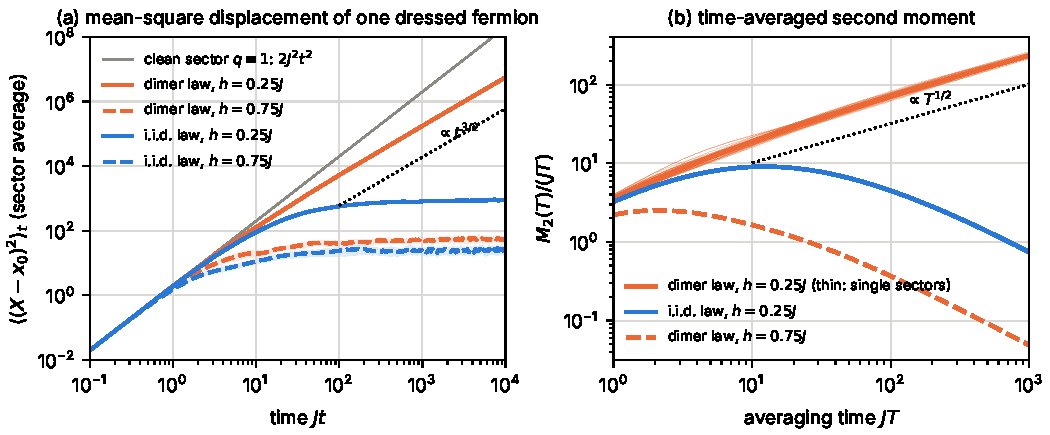
\includegraphics[width=\textwidth]{figs/dimer.pdf}
\caption{A single dressed fermion in the dimer state $\Psi^x=\cdr^\dagger_x\Omdim$ versus the i.i.d.\ law of
\cite{SKKM2017}, at $h=0.25J$ ($\lambda=0.5$, critical energies present) and $h=0.75J$
($\lambda=1.5$, none), with $J=1$.  The one-body dynamics is computed on $\Z$ (no boundary is reached)
and averaged over $64$ sectors.  (a) Sector-averaged mean-square
displacement $\langle(X-x)^2\rangle_t=D^{(N)}_2(t;x)$ in the thermodynamic limit, with bands of $\pm2$
standard errors.  The grey line is the clean sector $q\equiv1$ ($2J^2t^2$, \cref{rem:gaussproj}); the
dotted line has slope $3/2$.  (b) The
time average $\Mom_2(T)/(JT)$ of \cref{thm:dimer}.  Thin lines are the $64$ individual dimer sectors
at $h=0.25J$; each stays bounded below, as \cref{prop:dimerlower} asserts for every configuration, and
their mean grows roughly like $T^{1/2}$ (dotted), consistent with \cref{thm:dimer}(c).  For the
i.i.d.\ law, and for the dimer law at $h=0.75J$, $\Mom_2(T)$ saturates.  Code:
\texttt{code/dimer\_spread.py}; numerical values in \texttt{code/dimer\_spread.out}.}
\label{fig:dimer}
\end{figure}

\begin{remark}[Numerical illustration]\label{rem:dimernumerics}
\Cref{fig:dimer} shows the sector-averaged mean-square displacement of one dressed fermion for the
dimer law and the i.i.d.\ law, at $h=0.25J$ and $h=0.75J$, each averaged over $64$ sectors.  The
one-body dynamics is computed on $\Z$ by Chebyshev propagation on an adaptive window, which contains
every site where the wave function exceeds $10^{-18}$.  So no boundary is ever reached (the largest
window has $3.7\times10^4$ sites), and the data represent the thermodynamic limit of
\cref{thm:dimer}(b).  The propagation agrees with exact diagonalization to $3\times10^{-15}$, and the
norm is conserved to $3\times10^{-12}$.
\begin{itemize}
\item \emph{Dimer law, $h=0.25J$} ($\lambda=\frac12$, critical energies $\pm\lambda$):
$\langle(X-x)^2\rangle_t\approx1.3\times10^2$, $5.3\times10^3$, $1.8\times10^5$ and $5.6\times10^6$ at $Jt=10$,
$10^2$, $10^3$ and $10^4$.  The local exponents over the three decades are $1.62$, $1.52$ and $1.50$, in
line with the $t^{3/2}$ law of \cite{DWP1990} and with the exponent of \cref{thm:dimer}(c).
\item \emph{Saturation.}  For the i.i.d.\ law at $h=0.25J$ the same quantity saturates at
$\approx8.6\times10^2$.  At $h=0.75J$ ($\lambda=1.5$, covered by \cite[Thm.~2.3]{DeBievreGerminet2000},
\cref{rem:dimerstrong}) it saturates at $\approx50$ for the dimer law and at $\approx25$ for the i.i.d.\ law.
\item \emph{Time averages.}  In panel (b), $\Mom_2(T)$ is computed from the same data by the trapezoidal
rule.  On a finite chain this agrees with the exact eigenfunction formula to a relative error of
$10^{-4}$.  For the dimer law at $h=0.25J$, $\Mom_2(T)/(JT)\approx3.6$, $19$, $72$ and $2.3\times10^2$ at
$JT=1$, $10$, $10^2$ and $10^3$.  The smallest value over the $64$ sectors is $3.2$, $16$, $62$ and
$2.1\times10^2$.
\end{itemize}
These numbers illustrate \cref{thm:dimer}; they are not used in any proof.  The check script of
\cref{rem:dimerED} also tests \cref{lem:dimercritical}: the classification (ii) for $13$
values of $\lambda\in(0,3]$, the identities \eqref{eq:dimerrot} to $3\times10^{-15}$, the values
\eqref{eq:dimerangles} (computed independently from the eigenvalues of $D_-(\lambda)$), the commutator
formula (i) on a grid of energies, and the absence of critical energies for the anti-dimer law of
\cref{rem:dimersigns}.  It checks the bound \eqref{eq:dimerTbound} on $120$ random configurations,
alignments, energies and segments; the largest ratio of the two sides is $0.16$.  It verifies
\eqref{eq:quadid} to $10^{-15}$, \eqref{eq:dimerimbid} to $4\times10^{-14}$ ($100$ configurations,
$N=200$), and the Plancherel formula \eqref{eq:plancherel} to $10^{-8}$.  Finally, it checks
\eqref{eq:dimerlower} on a chain of $600$ sites for random, clean and periodic dimer configurations;
there the left side exceeds $c_{\lambda,2}T$ by a factor of at least $10^8$.
\end{remark}

\begin{remark}[Summary: the role of the initial state]\label{rem:dimermessage}
The Hamiltonian, the duality and the gauge-invariant observables are the same throughout this section.
For the $z$-polarized state of \cite{SKKM2017} the charges are i.i.d., and
Theorem~\ref{thm:EC} gives uniform, sector-averaged dynamical localization for every $h\neq0$
(\cref{sec:main}).  For the dimer states, which differ only in the orientation of the even links,
the charges come in neutral pairs.  For $0<2|h|<J$ transport is then at least diffusive in every
sector and superdiffusive on average (\cref{thm:dimer}), and for every $h\neq0$ the infinite-time
average of the CDW imbalance vanishes in the thermodynamic limit (\cref{prop:dimerimbalance}).  In the language of disordered systems, the initial state
selects the statistics of the effective disorder.  Correlations of the dimer type are known to produce
anomalous, superdiffusive transport \cite{DWP1990,JSBS2003}, although the spectrum remains almost surely
pure point \cite{DeBievreGerminet2000} (\cref{rem:dimerstrong}(iii)).  The strictly gauge-invariant sector $q\equiv1$ is not
localized at all (\cref{rem:gaussproj}).  Disorder-free localization is
therefore a joint property of the Hamiltonian and of the sector law induced by the initial state.
\end{remark}

% ---------------------------------------------------------------------------
% Section: Two dimensions
% ---------------------------------------------------------------------------
% Section-local macros (unique names, \providecommand only).
\providecommand{\TLat}{\mathcal{L}}          % finite graph (V,E)
\providecommand{\TCyc}{\mathcal{Z}}          % cycle space
\providecommand{\TFlux}{\Phi}                % flux configurations
\providecommand{\TGauge}{\Theta}             % gauge group {+-1}^V
\providecommand{\Tpi}{\pi}                   % fermion parity label
\providecommand{\Tclus}{\mathcal{C}}         % equal-charge cluster

\section{Two dimensions}\label{sec:2d}

The model of \cite{SKKM2018} is defined on an arbitrary graph.  In this section we prove the exact
free-fermion mapping on every finite connected graph, with the complete list of superselection labels
(charges, fluxes through plaquettes and, on a torus, the non-contractible Wilson loops) and the parity
constraint (\cref{thm:2dmap}).  We then determine the sector laws of two families of product initial
states (\cref{prop:2dlaws}): $\sigma^z$-polarized links give the two-dimensional Anderson model with
Bernoulli potential, and $\sigma^x$-polarized links with a checkerboard charge-density wave give binary
random $\pi$-flux with a staggered potential.  At strong coupling we prove a cluster-confinement estimate,
valid up to times of order $h/J^2$ (\cref{prop:cluster}), and we explain why it cannot be pushed further.
Finally we summarize what is (not) known about the two-dimensional one-body problems.  In contrast to one
dimension, we do \emph{not} obtain sector-averaged localization for any $h$ in two dimensions: the
required one-body input is not available (\cref{sec:2d:status}).

\subsection{The model on a graph and the exact mapping}\label{sec:2d:model}

\paragraph{Setting.}
Let $\TLat=(V,E)$ be a finite connected graph without loops; multiple edges are allowed.  Every edge
$b\in E$ has two distinct endpoints, $\partial b=\{i,j\}$, and we write $b\ni i$ if $i\in\partial b$.
The sites carry spinless fermions $f_i$, $i\in V$, with Fock space $\cF_V$, $n_i=f_i^\dagger f_i$ and
$N_f=\sum_in_i$; after fixing an enumeration of $V$, the occupation basis $\ket n$, $n\in\{0,1\}^V$, is
defined by the ordering convention \eqref{eq:occbasis}, and we write $\abs n:=\sum_in_i$.  We denote by
$\cF_V^{(\Tpi)}$, $\Tpi=\pm1$, the eigenspaces of the fermion parity $(-1)^{N_f}$.  The edges carry spins
$\frac12$; $\ket s_z$, $s\in\{\pm1\}^E$, is the $\sigma^z$-basis, and $\ket{n,s}:=\ket n\otimes\ket s_z$.
For $J>0$ and $h\in\R\setminus\{0\}$ let
\begin{equation}\label{eq:H2d}
  H_\TLat:=-J\sum_{b\in E,\ \partial b=\{i,j\}}\sigma^z_b\bigl(f_i^\dagger f_j+f_j^\dagger f_i\bigr)
  -h\sum_{i\in V}A_i,\qquad A_i:=\prod_{b\ni i}\sigma^x_b ,
\end{equation}
and define the Gauss operators and Wilson loops
\begin{equation}\label{eq:G2d}
  G_i:=(-1)^{n_i}A_i\quad(i\in V),\qquad W_\gamma:=\prod_{b\in\gamma}\sigma^z_b\quad(\gamma\in\TCyc(\TLat)).
\end{equation}
Here $\TCyc(\TLat)$ is the \emph{cycle space}: the set of edge sets $\gamma\subset E$ such that every
vertex is an endpoint of an even number of edges of $\gamma$.  It is a vector space over $\mathbb F_2$
under symmetric difference.  \eqref{eq:H2d} is \cite[Eqs.~(1)--(2)]{SKKM2018} with $J_{jk}\equiv J$ and
$h_j\equiv h$ (their sum over $\langle jk\rangle$ contains both orientations); $G_i$ is their conserved
charge $\hat q_i=(-1)^{\hat n_i}\hat A_i$, and $W_\gamma$ is their plaquette operator $\hat B_p$ when $\gamma$
is a plaquette and their Wilson loop $\hat\Gamma_n$ (their Eq.~(6)) when $\gamma$ winds around a torus.  For
the square lattice with open boundaries the $A_i$ of boundary sites are the ``incomplete stars'' of
\cite[Fig.~1]{SKKM2018}.  On a path with $N$ sites and $N-1$ links, \eqref{eq:H2d} is the ``open'' chain
of \cref{rem:boundary}(d); the boundary link of \cref{sec:model} is a one-dimensional device that we do
not use here.

\paragraph{Fluxes, gauge transformations, one-body operators.}
Let $\beta:=\abs E-\abs V+1$.  A \emph{flux configuration} is a group homomorphism
$\varphi:\TCyc(\TLat)\to\{\pm1\}$; they form a group $\TFlux(\TLat)$.  A sign configuration
$s\in\{\pm1\}^E$ has the flux $\varphi_s(\gamma):=\prod_{b\in\gamma}s_b$.  The gauge group
$\TGauge:=\{\pm1\}^V$ acts on sign configurations by $(\theta\cdot s)_b:=\theta_i\theta_js_b$ for
$\partial b=\{i,j\}$.  For $q\in\{\pm1\}^V$ and $s\in\{\pm1\}^E$ we define on $\ell^2(V)$
\begin{equation}\label{eq:hqs}
  K_s:=-J\sum_{b\in E,\ \partial b=\{i,j\}}s_b\bigl(\ket i\bra j+\ket j\bra i\bigr),\qquad
  h_{q,s}:=K_s+2h\,\diag(q),
\end{equation}
the hopping operator with binary $\pi$-fluxes $\varphi_s$ and the binary potential $\pm2h$.  With
$D_\theta:=\diag(\theta)$ one has $D_\theta h_{q,s}D_\theta=h_{q,\theta\cdot s}$, so by
\cref{lem:2dgauge}(i) the spectrum of $h_{q,s}$ and the moduli $\abs{f(h_{q,s})_{xy}}$ depend on $s$ only
through $\varphi_s$.  As in \cref{sec:model}, $\dGamma(a):=\sum_{x,y\in V}a_{xy}f_x^\dagger f_y$, and
$\Gamma(u)$ is the second quantization of a unitary $u$.

\begin{lemma}[Fluxes and gauge orbits]\label{lem:2dgauge}
\leavevmode
\begin{enumerate}[label=(\roman*)]
\item For $s,s'\in\{\pm1\}^E$: $\varphi_s=\varphi_{s'}$ if and only if $s'=\theta\cdot s$ for some
$\theta\in\TGauge$, and $\theta$ is then unique up to a global sign.
\item Let $T\subset E$ be a spanning tree.  For $b\in E\setminus T$ let $\gamma_b$ be the edge set
consisting of $b$ and the path in $T$ joining the endpoints of $b$.  Then
$\{\gamma_b:b\in E\setminus T\}$ is a basis of $\TCyc(\TLat)$; in particular
$\dim_{\mathbb F_2}\TCyc(\TLat)=\beta$ and $\abs{\TFlux(\TLat)}=2^\beta$.
\item The map $s\mapsto\varphi_s$ is onto $\TFlux(\TLat)$, and each fibre
$O_\varphi:=\{s:\varphi_s=\varphi\}$ is a $\TGauge$-orbit with $2^{\abs V-1}$ elements.
\end{enumerate}
\end{lemma}

\begin{proof}
(ii) Each $\gamma_b$ is a cycle (every vertex of a simple closed path has degree $2$), and $\gamma_b$ is the
only one of these sets containing the non-tree edge $b$; hence they are linearly independent.  Given
$\gamma\in\TCyc$, the set $\gamma':=\gamma\,\triangle\,\triangle_{b\in\gamma\setminus T}\gamma_b$ is a cycle
contained in $T$.  A non-empty edge set in a tree has a vertex of degree one (an endpoint of a longest
path in it), so $\gamma'=\emptyset$, and $\gamma=\triangle_{b\in\gamma\setminus T}\gamma_b$.  Since
$\abs T=\abs V-1$, $\dim\TCyc=\abs{E\setminus T}=\beta$; a homomorphism to $\{\pm1\}$ is determined by
its arbitrary values on a basis, so $\abs{\TFlux}=2^\beta$.

(i) If $s'=\theta\cdot s$ and $\gamma\in\TCyc$, then
$\varphi_{s'}(\gamma)=\varphi_s(\gamma)\prod_{i\in V}\theta_i^{d_\gamma(i)}=\varphi_s(\gamma)$, where the
degree $d_\gamma(i)$ of $i$ in $\gamma$ is even.  Conversely let $\varphi_s=\varphi_{s'}$ and $r:=ss'$
(pointwise), so that $\varphi_r\equiv1$.  Fix a root $v_0$ and define $\theta_v:=\prod_{b\in T(v_0,v)}r_b$,
the product over the tree path from $v_0$ to $v$.  For an edge $b$ with $\partial b=\{i,j\}$, if $b\in T$
then $T(v_0,i)\triangle T(v_0,j)=\{b\}$; if $b\notin T$ then $T(v_0,i)\triangle T(v_0,j)\triangle\{b\}=\gamma_b$.
In both cases $r_b=\prod_{T(v_0,i)\triangle T(v_0,j)}r=\theta_i\theta_j$ (use $r^2=1$ and
$\varphi_r(\gamma_b)=1$), i.e.\ $s'=\theta\cdot s$.  If $\theta\cdot s=\theta'\cdot s$, then
$(\theta\theta')_i=(\theta\theta')_j$ for every edge, so $\theta\theta'$ is constant because $\TLat$ is
connected.

(iii) Given $\varphi$, set $s_b:=1$ for $b\in T$ and $s_b:=\varphi(\gamma_b)$ for $b\notin T$; then
$\varphi_s=\varphi$ on the basis of (ii), hence everywhere.  By (i) the fibres are orbits, and the
stabilizer of every $s$ is $\{\pm(1,\dots,1)\}$, so each orbit has $2^{\abs V}/2$ elements.
\end{proof}

\begin{theorem}[Exact mapping on graphs; planar boxes and tori]\label{thm:2dmap}
Let $\TLat=(V,E)$ be a finite connected graph without loops.
\begin{enumerate}[label=(\alph*)]
\item The $G_i$ ($i\in V$) and $W_\gamma$ ($\gamma\in\TCyc(\TLat)$) are self-adjoint unitaries; they commute
with each other, with $N_f$ and with $H_\TLat$; and
\begin{equation}\label{eq:2dparity}
  \prod_{i\in V}G_i=(-1)^{N_f}.
\end{equation}
\item For $q\in\{\pm1\}^V$ and $\varphi\in\TFlux(\TLat)$ let $P_{q,\varphi}$ be the joint spectral projection
onto $\{G_i=q_i\ \forall i,\ W_\gamma=\varphi(\gamma)\ \forall\gamma\}$, and let $\Tpi_q:=\prod_iq_i$.  Then
$\sum_{q,\varphi}P_{q,\varphi}=\one$, $\operatorname{rank}P_{q,\varphi}=2^{\abs V-1}$ for \emph{every}
$(q,\varphi)$, and $(-1)^{N_f}P_{q,\varphi}=\Tpi_qP_{q,\varphi}$.  For every $s$ with $\varphi_s=\varphi$ there
is a unitary $V_{q,s}:\cF_V^{(\Tpi_q)}\to\operatorname{Ran}P_{q,\varphi}$ which maps each $\ket n$ to a joint
eigenvector of the $n_i$ with the same eigenvalues, and such that, on $\cF_V^{(\Tpi_q)}$,
\begin{equation}\label{eq:2ddict}
  V_{q,s}^*\,\sigma^z_bf_i^\dagger f_j\,V_{q,s}=s_b\,f_i^\dagger f_j\quad(\partial b=\{i,j\}),\qquad
  V_{q,s}^*A_iV_{q,s}=q_i(-1)^{n_i},
\end{equation}
and consequently
\begin{equation}\label{eq:2dsector}
  V_{q,s}^*\,H_\TLat\,V_{q,s}=\Bigl(\dGamma(h_{q,s})-h\sum_{i\in V}q_i\Bigr)\Big|_{\cF_V^{(\Tpi_q)}} .
\end{equation}
For $\theta\in\TGauge$, $V_{q,\theta\cdot s}=q(\theta)\,V_{q,s}\,\Gamma(D_\theta)$ with
$q(\theta):=\prod_{i:\theta_i=-1}q_i$.
\item \emph{Planar box.}  Let $\TLat$ be the box $\{1,\dots,L_1\}\times\{1,\dots,L_2\}$ with nearest-neighbour
edges, and let the plaquettes $p$ be its unit squares, with boundaries $\partial p$ and $W_p:=W_{\partial p}$.
Then $\beta=(L_1-1)(L_2-1)$, and $\{\partial p\}_p$ is a basis of $\TCyc(\TLat)$.  Hence the sectors are
labelled by $(q,(W_p)_p)\in\{\pm1\}^V\times\{\pm1\}^{\#\text{plaquettes}}$, all $2^{\abs V+\beta}$ labels
occur, and in the sector $(q,(W_p))$ the matter consists of free fermions with the binary potential $2hq_i$
and the binary $\pi$-flux $W_p=\prod_{b\in\partial p}s_b\in\{\pm1\}$ through $p$, restricted to the parity
sector $(-1)^{N_f}=\prod_iq_i$.
\item \emph{Torus.}  Let $\TLat$ be the torus $(\Z/L_1\Z)\times(\Z/L_2\Z)$, $L_1,L_2\ge3$, with
nearest-neighbour edges, plaquettes $p$ as in (c), and let $\gamma_1$ (resp.\ $\gamma_2$) be the set of
horizontal edges of the row $\{y=0\}$ (resp.\ the vertical edges of the column $\{x=0\}$).  Then
$\beta=L_1L_2+1$, $\prod_pW_p=\one$, and $\{\partial p:p\neq p_0\}\cup\{\gamma_1,\gamma_2\}$ is a basis of
$\TCyc(\TLat)$ for any fixed plaquette $p_0$.  Hence the sectors are labelled by $q$, the plaquette fluxes
$(W_p)_p$ subject to $\prod_pW_p=1$, and the two non-contractible Wilson loops $W_{\gamma_1},W_{\gamma_2}$,
which are independent labels; all $2^{\abs V+\beta}$ labels occur, and in $h_{q,s}$ the non-contractible
loops act as $\Z_2$ twists of the boundary conditions in the two directions.
\end{enumerate}
\end{theorem}

\begin{proof}
For $\theta\in\TGauge$ let $V_\theta:=\{i:\theta_i=-1\}$, $q(\theta):=\prod_{i\in V_\theta}q_i$,
$\varepsilon_n(\theta):=\prod_{i\in V_\theta}(-1)^{n_i}$ and $\mathcal G_\theta:=\prod_{i\in V_\theta}G_i$.
Since $\sigma^x$ flips $\sigma^z$-eigenstates and $\TLat$ has no loops, $A_i\ket{n,s}=\ket{n,\theta^{(i)}\cdot s}$,
where $\theta^{(i)}$ equals $-1$ at $i$ only.  Hence
\begin{equation}\label{eq:Gtheta}
  \mathcal G_\theta\ket{n,s}=\varepsilon_n(\theta)\,\ket{n,\theta\cdot s}\qquad(\theta\in\TGauge).
\end{equation}

(a) $G_i$ and $W_\gamma$ are products of commuting self-adjoint unitaries.  The $G_i$ are built from the
mutually commuting operators $\sigma^x_b$ and $(-1)^{n_k}$; the $W_\gamma$ are diagonal in the basis
$\ket{n,s}$, so they commute with each other, with $N_f$ and with every $(-1)^{n_k}$; and
$A_iW_\gamma=(-1)^{d_\gamma(i)}W_\gamma A_i=W_\gamma A_i$ because the degree $d_\gamma(i)$ is even.  The
electric term commutes with all $\sigma^x_b$, $(-1)^{n_k}$ and $W_\gamma$.  Let
$T_b:=\sigma^z_b(f_i^\dagger f_j+f_j^\dagger f_i)$, $\partial b=\{i,j\}$.  It commutes with every
$W_\gamma$.  It anticommutes with $A_k$ iff $b\ni k$, and with $(-1)^{n_k}$ iff $k\in\{i,j\}$ (because
$(-1)^{n_i}f_i^\dagger=-f_i^\dagger(-1)^{n_i}$ and $(-1)^{n_i}$ commutes with $f_j$, $j\ne i$); so it
commutes with each $G_k=(-1)^{n_k}A_k$.  Everything commutes with $N_f$.  Finally
$\prod_iG_i=(-1)^{N_f}\prod_iA_i=(-1)^{N_f}\prod_{b\in E}(\sigma^x_b)^2=(-1)^{N_f}$, since every edge has
exactly two endpoints.

(b) \emph{Step 1: joint eigenvectors.}  Let $P_q:=\prod_i\frac12(\one+q_iG_i)=2^{-\abs V}\sum_{\theta\in\TGauge}q(\theta)\mathcal G_\theta$.
By \eqref{eq:Gtheta}, $P_q\ket{n,s}=2^{-\abs V}\sum_\theta q(\theta)\varepsilon_n(\theta)\ket{n,\theta\cdot s}$.  The
elements $\theta$ and $-\theta$ give the same vector $\ket{n,\theta\cdot s}$, and
$q(-\theta)\varepsilon_n(-\theta)=\Tpi_q(-1)^{\abs n}q(\theta)\varepsilon_n(\theta)$.  Hence $P_q\ket{n,s}=0$ if
$(-1)^{\abs n}\neq\Tpi_q$, while for $(-1)^{\abs n}=\Tpi_q$
\begin{equation}\label{eq:Psi2d}
  \Psi_{n,q,s}:=2^{(\abs V-1)/2}P_q\ket{n,s}
  =2^{-(\abs V-1)/2}\sum_{[\theta]\in\TGauge/\{\pm1\}}q(\theta)\varepsilon_n(\theta)\,\ket{n,\theta\cdot s},
\end{equation}
where the summand depends only on the class $[\theta]=\{\theta,-\theta\}$.  By \cref{lem:2dgauge}(i),(iii),
$[\theta]\mapsto\theta\cdot s$ is a bijection onto the orbit $O_{\varphi_s}$, so \eqref{eq:Psi2d} is a normalized
sum of $2^{\abs V-1}$ orthonormal vectors with unimodular coefficients: $\Psi_{n,q,s}$ is a unit vector.  It
satisfies $G_i\Psi_{n,q,s}=q_i\Psi_{n,q,s}$ (as $G_iP_q=q_iP_q$), $W_\gamma\Psi_{n,q,s}=\varphi_s(\gamma)\Psi_{n,q,s}$
(every $\ket{n,\theta\cdot s}$ has flux $\varphi_s$), and it is an eigenvector of every occupation operator, with
the same eigenvalues as $\ket n$.

\emph{Step 2: orthonormal bases.}  Fix $\varphi$ and $s\in O_\varphi$.  Since the $W_\gamma$ are diagonal in the
basis $\ket{n,s'}$, their joint eigenspace with eigenvalues $\varphi$ is spanned by $\{\ket{n,s'}:s'\in O_\varphi\}$.
The joint eigenvalues of the commuting self-adjoint unitaries $(W_\gamma)_\gamma$ form a homomorphism
$\gamma\mapsto\varphi(\gamma)$, because $W_{\gamma\triangle\gamma'}=W_\gamma W_{\gamma'}$; hence
$\sum_{q,\varphi}P_{q,\varphi}=\one$.  As $P_q$ commutes with the $W_\gamma$, $\operatorname{Ran}P_{q,\varphi}$ is
spanned by the vectors $P_q\ket{n,\theta\cdot s}$, $\theta\in\TGauge$.  By \eqref{eq:Gtheta},
$\ket{n,\theta\cdot s}=\varepsilon_n(\theta)\mathcal G_\theta\ket{n,s}$, and $P_q\mathcal G_\theta=q(\theta)P_q$, so
\begin{equation}\label{eq:Psigauge}
  P_q\ket{n,\theta\cdot s}=q(\theta)\varepsilon_n(\theta)\,P_q\ket{n,s}.
\end{equation}
Therefore $\{\Psi_{n,q,s}:(-1)^{\abs n}=\Tpi_q\}$ spans $\operatorname{Ran}P_{q,\varphi}$; it is orthonormal because
distinct $n$ give orthogonal vectors.  This proves $\operatorname{rank}P_{q,\varphi}=2^{\abs V-1}$ and
$(-1)^{N_f}=\Tpi_q$ on $\operatorname{Ran}P_{q,\varphi}$, and $V_{q,s}\ket n:=\Psi_{n,q,s}$ defines a unitary
$\cF_V^{(\Tpi_q)}\to\operatorname{Ran}P_{q,\varphi}$.  By \eqref{eq:Psigauge},
$\Psi_{n,q,\theta\cdot s}=q(\theta)\varepsilon_n(\theta)\Psi_{n,q,s}$, which is the stated change of representative,
since $\Gamma(D_\theta)\ket n=\varepsilon_n(\theta)\ket n$.

\emph{Step 3: the Hamiltonian.}  Since $A_i=(-1)^{n_i}G_i$, $A_i\Psi_{n,q,s}=q_i(-1)^{n_i}\Psi_{n,q,s}$.  For the
hopping let $\partial b=\{i,j\}$ and $n_j=1$, $n_i=0$, so that $f_i^\dagger f_j\ket n=\eta\ket{n'}$ with
$n':=n-e_j+e_i$ and a sign $\eta$ given by \eqref{eq:fsign}; if $n_j=0$ or $n_i=1$ then $f_i^\dagger f_j\ket n=0$.
As $n'$ and $n$ differ exactly at $i$ and $j$, $\varepsilon_{n'}(\theta)=\theta_i\theta_j\varepsilon_n(\theta)$, and
$\sigma^z_b\ket{\theta\cdot s}_z=\theta_i\theta_js_b\ket{\theta\cdot s}_z$.  Hence, by \eqref{eq:Psi2d},
\[
  \sigma^z_bf_i^\dagger f_j\,\Psi_{n,q,s}
  =2^{-(\abs V-1)/2}\sum_{[\theta]}q(\theta)\varepsilon_n(\theta)\theta_i\theta_js_b\,\eta\,\ket{n',\theta\cdot s}
  =s_b\,\eta\,\Psi_{n',q,s},
\]
and both sides vanish in the remaining cases.  This is \eqref{eq:2ddict}.  Summing,
$V_{q,s}^*H_\TLat V_{q,s}=-J\sum_bs_b(f_i^\dagger f_j+f_j^\dagger f_i)-h\sum_iq_i(1-2n_i)$, which is
\eqref{eq:2dsector}.

(c) The box is connected, $\abs V=L_1L_2$ and $\abs E=(L_1-1)L_2+L_1(L_2-1)$, so $\beta=(L_1-1)(L_2-1)$, the
number of plaquettes.  Each $\partial p$ is a cycle.  If $\triangle_{p\in P'}\partial p=\emptyset$ for a non-empty set
$P'$ of plaquettes, pick $p\in P'$ whose lower-left corner has maximal first coordinate; the right edge of $p$
lies in $\partial p$ and otherwise only in the boundary of the plaquette to the right of $p$, which is not in
$P'$, so it survives in the symmetric difference, a contradiction.  So the $\partial p$ are $\beta$ independent
vectors, hence a basis, and $\varphi\mapsto(\varphi(\partial p))_p$ is a bijection
$\TFlux\to\{\pm1\}^{\#\text{plaquettes}}$.  The rest follows from (b).

(d) For $L_1,L_2\ge3$ the torus is a simple $4$-regular connected graph with $\abs V=L_1L_2$ and $\abs E=2L_1L_2$,
so $\beta=L_1L_2+1$.  Every edge lies in exactly two plaquettes, so $\triangle_p\partial p=\emptyset$, i.e.\
$\prod_pW_p=\one$.  If $\triangle_{p\in P'}\partial p=\emptyset$ with $\emptyset\neq P'\neq$ all plaquettes, then,
the dual torus being connected, some edge lies in a plaquette of $P'$ and in one outside $P'$, and survives:
a contradiction.  Hence the $\partial p$, $p\ne p_0$, are independent and span the same space $B$ as all
$\partial p$.  Let $C_1$ be the set of horizontal edges joining $(0,y)$ and $(1,y)$, $y\in\Z/L_2\Z$, and $C_2$
the set of vertical edges joining $(x,0)$ and $(x,1)$.  The linear forms $\ell_k(\gamma):=\abs{\gamma\cap C_k}\bmod2$
vanish on every $\partial p$ (a plaquette contains $0$ or $2$ edges of $C_k$), and
$\ell_1(\gamma_1)=\ell_2(\gamma_2)=1$, $\ell_1(\gamma_2)=\ell_2(\gamma_1)=0$.  Hence $\gamma_1,\gamma_2$ are independent
modulo $B$, and $\{\partial p:p\ne p_0\}\cup\{\gamma_1,\gamma_2\}$ consists of $L_1L_2+1=\beta$ independent cycles, a
basis.  Choosing $s$ as in \cref{lem:2dgauge}(iii), $W_{\gamma_1}$ and $W_{\gamma_2}$ are the products of the hopping
signs around the two non-contractible directions, i.e.\ twisted boundary conditions.
\end{proof}

\begin{remark}[Comparison with \cite{SKKM2018}]\label{rem:2dSKKM}
SKKM introduce dual spins by $\hat\tau^z_j=\hat A_j$, $\hat\tau^x_j\hat\tau^x_k=\hat\sigma^z_{jk}$
\cite[Eq.~(5)]{SKKM2018}, which forces $\hat B_p=1$ and $\hat\Gamma_n=1$; other Wilson-loop sectors are reached by
modifying the duality along reference lines \cite[Eq.~(19)]{SKKM2018}, and the global constraint
$\prod_i\hat q_i=(-1)^{\hat N_f}$ is their Eq.~(7).  \Cref{thm:2dmap} treats all sectors at once: the dimension
count $2^{\abs V}\cdot2^\beta\cdot2^{\abs V-1}=2^{\abs V+\abs E}$ shows that the labels $(q,\varphi)$ exhaust
$\cH$, every sector $(q,\varphi)$ carries the free-fermion Hamiltonian $\dGamma(h_{q,s})$, $s\in O_\varphi$, on the
parity sector $\Tpi_q$, and the only constraint is the parity relation \eqref{eq:2dparity}.  Unlike in the chain with a boundary link
(\cref{lem:gauss}), the charges of a graph without ``dangling'' links can never be independent of the matter
parity.
\end{remark}

\subsection{Sector laws of product initial states}\label{sec:2d:laws}

For an operator $O$ on $\cH$ commuting with all $G_i$ and all $W_\gamma$ we write
$O_{q,s}:=V_{q,s}^*OV_{q,s}$, an operator on $\cF_V^{(\Tpi_q)}$; for every function $F$ of the occupation
numbers, $F_{q,s}=F$.  We write $\Psi(t):=\e^{-\ii tH_\TLat}\Psi_0$.

\begin{proposition}[Sector laws]\label{prop:2dlaws}
Let $\TLat$ be as in \cref{thm:2dmap}.
\begin{enumerate}[label=(\alph*)]
\item \emph{$\sigma^z$-product links: the Anderson--Bernoulli model.}  Let $\Psi_0=\psi\otimes\ket{s}_z$ with
$s\in\{\pm1\}^E$ and $\psi\in\cF_V^{(\Tpi)}$ of definite parity $\Tpi$.  Then $P_{q,\varphi}\Psi_0=0$ unless
$\varphi=\varphi_s$ and $\Tpi_q=\Tpi$, and for these sectors $P_{q,\varphi_s}\Psi_0=2^{-(\abs V-1)/2}\,V_{q,s}\psi$.  So the
flux is deterministic, the sector law of the charges is uniform on the parity hyperplane $\{q:\prod_iq_i=\Tpi\}$,
every sector carries the matter state $\psi$, and for every $O$ commuting with all $G_i,W_\gamma$
\begin{equation}\label{eq:2dlawz}
  \langle\Psi(t),O\Psi(t)\rangle=2^{1-\abs V}\sum_{q:\ \prod_iq_i=\Tpi}
  \bigl\langle\Gamma(\e^{-\ii th_{q,s}})\psi,\,O_{q,s}\,\Gamma(\e^{-\ii th_{q,s}})\psi\bigr\rangle .
\end{equation}
The law of $q$ has density at most $2$ with respect to the i.i.d.\ Bernoulli$(1/2)$ law.  For the
$\sigma^z$-polarized state $\ket{\uparrow\cdots\uparrow}_z$, i.e.\ $s=+:=(1,\dots,1)$, all fluxes vanish and the
one-body operators are the Anderson--Bernoulli operators $h_{q,+}=-J\Delta+2h\diag(q)$, with $\Delta$ the adjacency
operator of $\TLat$.
\item \emph{$\sigma^x$-polarized links: random $\pi$-flux.}  Let $\Psi_0=\ket{n^0}\otimes\ket{+\cdots+}$, where
$\sigma^x_b\ket{+\cdots+}=\ket{+\cdots+}$ for all $b$.  Let $q^0_i:=(-1)^{n^0_i}$.  Then $P_{q,\varphi}\Psi_0=0$
unless $q=q^0$, and for every $\varphi\in\TFlux(\TLat)$ and every $s\in O_\varphi$,
$P_{q^0,\varphi}\Psi_0=2^{-\beta/2}\,V_{q^0,s}\ket{n^0}$.  So the charges are deterministic, the flux
configuration is uniformly distributed on $\TFlux(\TLat)$ (on a box: i.i.d.\ uniform plaquette fluxes; on a
torus: $(W_p)$ uniform on $\{\prod_pW_p=1\}$, and $W_{\gamma_1},W_{\gamma_2}$ independent and uniform), every sector
carries the matter state $\ket{n^0}$, and
\begin{equation}\label{eq:2dlawx}
  \langle\Psi(t),O\Psi(t)\rangle=2^{-\beta}\sum_{\varphi\in\TFlux}
  \bigl\langle\Gamma(\e^{-\ii th_{q^0,s^\varphi}})n^0,\,O_{q^0,s^\varphi}\,\Gamma(\e^{-\ii th_{q^0,s^\varphi}})n^0\bigr\rangle ,
  \qquad s^\varphi\in O_\varphi .
\end{equation}
\item \emph{Checkerboard.}  In (b) let $\TLat$ be bipartite with sublattice signs $\epsilon_i\in\{\pm1\}$
($\epsilon_i=-\epsilon_j$ whenever $\partial b=\{i,j\}$), and $n^0_i=\frac12(1+\epsilon_i)$.  Let
$\Gamma_\epsilon:=\diag(\epsilon)$.  Then $h_{q^0,s}=K_s-2h\Gamma_\epsilon$ with
$K_s\Gamma_\epsilon=-\Gamma_\epsilon K_s$, and for every $s$:
\begin{enumerate}[label=(\roman*)]
\item $h_{q^0,s}^2=K_s^2+4h^2$;
\item $\sigma(h_{q^0,s})\subset(-\infty,-2\abs h]\cup[2\abs h,\infty)$, and for every Borel set $B\subset[0,\infty)$,
$\one_B(\abs{h_{q^0,s}})=\one_{g^{-1}(B)}(\abs{K_s})$ with $g(e):=\sqrt{e^2+4h^2}$.  In particular
$\one_{\{2\abs h\}}(\abs{h_{q^0,s}})$ is the projection onto $\ker K_s$, and
$\one_{[2\abs h,\sqrt{4h^2+\delta^2}]}(\abs{h_{q^0,s}})=\one_{[0,\delta]}(\abs{K_s})$ for $\delta\ge0$: the
chiral point $E=0$ of the random-flux operator $K_s$ is mapped to the inner band edges $\abs E=2\abs h$;
\item with $R_s:=(K_s^2+4h^2)^{1/2}$, $\e^{-\ii th_{q^0,s}}=\cos(tR_s)-\ii\,h_{q^0,s}R_s^{-1}\sin(tR_s)$;
\item $(K_s^2)_{ii}=J^2\deg(i)$.  If $\TLat$ is a box in $\Z^2$, $K_s^2$ connects only sites of the same
sublattice at distance $2$: $(K_s^2)_{ik}=J^2s_{ij}s_{jk}$ if $k=i\pm2e_\mu$ (with midpoint $j$), and
$(K_s^2)_{ik}=J^2s_{ij_1}s_{j_1k}(1+W_p)$ if $i,k$ are opposite corners of the plaquette $p$ with the other
corners $j_1,j_2$; here $s_{ij}$ is the sign of the edge joining $i$ and $j$.  Thus the diagonal amplitudes of
$K_s^2$ vanish across $\pi$-flux plaquettes.
\end{enumerate}
\end{enumerate}
\end{proposition}

\begin{proof}
(a) $W_\gamma\Psi_0=\varphi_s(\gamma)\Psi_0$ for all $\gamma$, so $P_{q,\varphi}\Psi_0=0$ for $\varphi\neq\varphi_s$.  Write
$\psi=\sum_n\psi(n)\ket n$ with $(-1)^{\abs n}=\Tpi$.  By Step~1 of the proof of \cref{thm:2dmap},
$P_q\ket{n,s}=0$ if $\Tpi_q\neq\Tpi$ and $P_q\ket{n,s}=2^{-(\abs V-1)/2}\Psi_{n,q,s}=2^{-(\abs V-1)/2}V_{q,s}\ket n$
otherwise; sum over $n$.  Since $O$ commutes with all $P_{q,\varphi}$, and $\e^{-\ii tH_\TLat}$ commutes with them,
\[
  \langle\Psi(t),O\Psi(t)\rangle=\sum_q\langle P_{q,\varphi_s}\Psi(t),OP_{q,\varphi_s}\Psi(t)\rangle
  =2^{1-\abs V}\sum_{\Tpi_q=\Tpi}\langle\e^{-\ii tH_q}\psi,O_{q,s}\e^{-\ii tH_q}\psi\rangle,
\]
with $H_q:=\dGamma(h_{q,s})-h\sum_iq_i$ by \eqref{eq:2dsector}; the constant drops out, and
$\e^{-\ii t\dGamma(a)}=\Gamma(\e^{-\ii ta})$.  The uniform law on a hyperplane has density $2$ on its support.

(b) As $\sigma^x_b\ket{+\cdots+}=\ket{+\cdots+}$, $A_i\Psi_0=\Psi_0$, so $G_i\Psi_0=q^0_i\Psi_0$.  Expanding
$\ket{+\cdots+}=2^{-\abs E/2}\sum_s\ket s_z$, the $W$-eigenspace $\varphi$ receives
$P_{q^0,\varphi}\Psi_0=2^{-\abs E/2}\sum_{s'\in O_\varphi}\ket{n^0,s'}$.  For every $\theta$,
\[
  q^0(\theta)\,\varepsilon_{n^0}(\theta)=\prod_{i\in V_\theta}(-1)^{2n^0_i}=1,
\]
so by \eqref{eq:Psi2d} and \cref{lem:2dgauge}(iii),
$\Psi_{n^0,q^0,s}=2^{-(\abs V-1)/2}\sum_{s'\in O_\varphi}\ket{n^0,s'}$ for every $s\in O_\varphi$.  Hence $P_{q^0,\varphi}\Psi_0=2^{(\abs V-1-\abs E)/2}\Psi_{n^0,q^0,s}=2^{-\beta/2}V_{q^0,s}\ket{n^0}$.
The uniformity statements on boxes and tori follow from \cref{thm:2dmap}(c),(d), since the coordinates of a
uniformly distributed element of $\{\pm1\}^k$ with respect to a basis are i.i.d.\ uniform.  Formula
\eqref{eq:2dlawx} follows as in (a).

(c) Every edge joins opposite sublattices, so $\Gamma_\epsilon K_s\Gamma_\epsilon=-K_s$, and
$q^0_i=(-1)^{n^0_i}=-\epsilon_i$, so $h_{q^0,s}=K_s-2h\Gamma_\epsilon$.  (i)
$(K_s-2h\Gamma_\epsilon)^2=K_s^2-2h(K_s\Gamma_\epsilon+\Gamma_\epsilon K_s)+4h^2\Gamma_\epsilon^2=K_s^2+4h^2$.  (ii) By
(i), $h_{q^0,s}^2\ge4h^2$, which gives the spectral inclusion, and by the functional calculus
$\abs{h_{q^0,s}}=(K_s^2+4h^2)^{1/2}=g(\abs{K_s})$; hence $\one_B(\abs{h_{q^0,s}})=(\one_B\circ g)(\abs{K_s})
=\one_{g^{-1}(B)}(\abs{K_s})$.  Take $B=\{2\abs h\}$ and $B=[2\abs h,\sqrt{4h^2+\delta^2}]$, for which
$g^{-1}(B)=\{0\}$ and $[0,\delta]$.  (iii) For real $E\ne0$, $\e^{-\ii tE}=\cos(t\abs E)-\ii(E/\abs E)\sin(t\abs E)$;
apply the functional calculus to $h_{q^0,s}$, whose spectrum avoids $(-2\abs h,2\abs h)$, and use
$\abs{h_{q^0,s}}=R_s$.  (iv) $(K_s^2)_{ik}=J^2\sum_js_{ij}s_{jk}$, summed over the common neighbours $j$ of $i$
and $k$.  In a box these exist only for $k=i$ ($\deg(i)$ terms equal to $1$), for $k=i\pm2e_\mu$ (one common
neighbour), and for diagonal pairs, which have the two common neighbours $j_1,j_2$; then
$s_{ij_2}s_{j_2k}=W_p\,s_{ij_1}s_{j_1k}$ because $W_p=s_{ij_1}s_{j_1k}s_{kj_2}s_{j_2i}$ and $s^2=1$.
\end{proof}

\begin{remark}[Interpretation]\label{rem:2dlaws}
\leavevmode
\begin{enumerate}[label=(\alph*)]
\item \Cref{prop:2dlaws}(a) is the two-dimensional analogue of \cref{cor:sector}: for $\sigma^z$-polarized
links all gauge-invariant dynamics is an average over the zero-flux Anderson model $h_{q,+}=-J\Delta+2h\diag(q)$
with Bernoulli potential, restricted to a parity hyperplane of charge configurations.  This is the setting of
\cite{SKKM2018}.  A $\sigma^z$-product state with flipped links has the same charge law but a deterministic,
in general non-zero, flux $\varphi_s$; if $\varphi_s\equiv1$, then $s=\theta\cdot+$ for some $\theta$
(\cref{lem:2dgauge}), and by \cref{thm:2dmap}(b) the gauge-invariant dynamics is that of the polarized state with
the matter state $\Gamma(D_\theta)\psi$ (a sign for Fock $\psi$), as in \cref{lem:productlaw}(c).
\item In \cref{prop:2dlaws}(b) the disorder sits entirely in the fluxes, while the potential
$2h(-1)^{n^0_i}$ is fixed by the initial matter configuration.  The state $\ket{+\cdots+}$ has $A_i\equiv1$; the
toric-code ground states considered in \cite[Sect.~I.C]{SKKM2018} are its normalized projections onto single flux
sectors, in which neither the charges nor the fluxes are random.  For the checkerboard (c), the
sector-averaged dynamics is a function of the binary random $\pi$-flux operator $K_s$ alone, by (iii); in
particular every localization question for this initial state is a question about $K_s$ and $K_s^2$.  The
chiral point $E=0$ of $K_s$, where random-flux and random-hopping models are expected to be critical rather than
localized (the Gade singularity \cite{Gade1993}), sits at the inner band edges $\abs E=2\abs h$ of
$h_{q^0,s}$.  We know of no localization theorem for $K_s$ with i.i.d.\ binary fluxes at any energy
(\cref{sec:2d:status}).
\end{enumerate}
\end{remark}

\begin{remark}[Numerical verification]\label{rem:2dED}
The script
\begin{center}
\texttt{code/twod\_check.py}\quad(output: \texttt{code/twod\_check.out})
\end{center}
builds $H_\TLat$, the $G_i$ and the $W_\gamma$ from scratch in the basis $\ket{n,s}$ (Jordan--Wigner fermions, no input from the proof).
\begin{itemize}
\item \emph{\Cref{thm:2dmap}, sector by sector.}  For the planar $2\times3$ box ($\dim\cH=8192$), the
$2\times2$ torus (a multigraph with $\beta=5$: three independent plaquettes and two non-contractible loops;
$\dim\cH=4096$) and the complete graph $K_4$, the joint eigenspaces of all $G_i$ and of the fundamental-cycle
Wilson loops were computed by diagonalizing a random linear combination of them.  Exactly $2^{\abs V+\beta}$
sectors occur, each of dimension $\binom{\abs V}{N_f}$ in the $N_f$-particle space if
$\prod_iq_i=(-1)^{N_f}$ and empty otherwise, and the spectrum of $H_\TLat$ in each of them coincides with that
of $\dGamma(h_{q,s})-h\sum_iq_i$ with $s$ realizing the measured fluxes, to $2\times10^{-14}$ ($J=1$, $h=0.8$).
\item \emph{\Cref{prop:2dlaws}(a),(b).}  For the $2\times4$ and $3\times3$ boxes and the $2\times2$ torus, the
sector weights $\norm{P_{q,\varphi}\Psi_0}^2$ agree with (a) and (b) exactly, and the full time evolution of
$\langle n_x(t)\rangle$ for $t\le8$ ($h\in\{0.4,1.3\}$; checkerboard and other Fock states, both link
polarizations) agrees with \eqref{eq:2dlawz}, \eqref{eq:2dlawx} to $3\times10^{-13}$.
\item \emph{\Cref{prop:2dlaws}(c)} on a $16\times16$ box with random fluxes: (i), (iii) and the entries in (iv) to
$10^{-12}$, and $\min\abs{\sigma(h_{q^0,s})}\ge2\abs h$.
\end{itemize}
\end{remark}

\subsection{Strong coupling: cluster confinement up to times of order \texorpdfstring{$h/J^2$}{h/J²}}\label{sec:2d:strong}

Let $\Lambda\subset\Z^2$ be a box (or $\Lambda=\Z^2$), with nearest-neighbour edges $E(\Lambda)$, and let
$s\in\{\pm1\}^{E(\Lambda)}$, $q\in\{\pm1\}^\Lambda$ be arbitrary; $h_{q,s}=K_s+2h\diag(q)$ acts on $\ell^2(\Lambda)$ as
in \eqref{eq:hqs}.  The \emph{equal-charge clusters} are the connected components of the subgraphs of $\Lambda$
induced on $\{q=+1\}$ and on $\{q=-1\}$; $\Tclus_q(x)$ denotes the cluster containing $x$.  With
$P_\pm:=\one_{\{q=\pm1\}}$ let
\begin{equation}\label{eq:h0}
  h^0_{q,s}:=P_+h_{q,s}P_++P_-h_{q,s}P_-,\qquad h^1_{q,s}:=h_{q,s}-h^0_{q,s}=P_+h_{q,s}P_-+P_-h_{q,s}P_+ ,
\end{equation}
i.e.\ $h^0_{q,s}$ is $h_{q,s}$ with the hopping across all bonds joining opposite charges removed.  For
$x\in\Lambda$ and $R\ge0$ let $B_R(x):=\{y\in\Lambda:\abs{y-x}_\infty\le R\}$.

\begin{proposition}[Cluster confinement at strong coupling]\label{prop:cluster}
Assume $\abs h>2J$ and set $g:=4\abs h-8J>0$.
\begin{enumerate}[label=(\alph*)]
\item $h^0_{q,s}$ leaves $\ell^2(\Tclus)$ invariant for every equal-charge cluster $\Tclus$.
\item For all $t\in\R$, uniformly in $\Lambda$, $q$ and $s$,
\begin{equation}\label{eq:clusterbound}
  \norm{\e^{-\ii th_{q,s}}-\e^{-\ii th^0_{q,s}}}\le\frac{8J}{g}+\frac{48\,\abs t\,J^2}{g} .
\end{equation}
Consequently, for every $x\in\Lambda$, $\norm{\one_{\Lambda\setminus\Tclus_q(x)}\e^{-\ii th_{q,s}}\delta_x}\le8J/g+48\abs tJ^2/g$.
\item Let the law of $q$ have density at most $K$ with respect to the i.i.d.\ Bernoulli$(1/2)$ law on
$\{\pm1\}^\Lambda$ ($K=1$ for i.i.d.\ charges, $K=2$ for the parity hyperplane of \cref{prop:2dlaws}(a)).
There is a numerical constant $c_*>0$ such that for all $x\in\Lambda$, $R\ge4$, $t\in\R$ and $s$,
\begin{equation}\label{eq:clusterprob}
  \E\,\norm{\one_{\Lambda\setminus B_R(x)}\,\e^{-\ii th_{q,s}}\delta_x}^2
  \le\Bigl(\frac{8J}{g}+\frac{48\,\abs t\,J^2}{g}\Bigr)^2+2K\,\e^{-c_*(2R+3)} .
\end{equation}
\end{enumerate}
\end{proposition}

The constant $c_*$ is the one of \cite[Prop.~2.2]{LiL2022}, which rests on $p_c^{\rm site}(\Z^2)>\frac12$
\cite{GrimmettStacey1998} and on the sharpness of the phase transition \cite[Thm.~7.3]{AizenmanBarsky1987};
we quote it in the proof.  No smallness condition on $J/g$ is needed for (b): the bound is proved for all
$\abs h>2J$.  It is informative only when its right-hand side is below $2$, which requires $J/g<\frac14$ and
$\abs t<(2g-8J)/(48J^2)$; in the complementary range (in particular for $J/g\ge\frac14$) it holds trivially,
since the left-hand side never exceeds $2$.  We made no attempt to optimize the constants $8$ and $48$.

\begin{proof}
Replacing $(h,q)$ by $(-h,-q)$ changes neither $h_{q,s}$, $h^0_{q,s}$ nor the clusters, and preserves the laws in
(c); so let $h>0$.  Write $h=h_{q,s}$, $h^0=h^0_{q,s}$, $h^1=h^1_{q,s}$, and let $h^0_\pm:=P_\pm hP_\pm$, regarded as
operators on $\operatorname{Ran}P_\pm$.

(a) The off-diagonal entries of $h^0$ join nearest neighbours of equal charge only; hence
$\langle\delta_y,h^0\delta_x\rangle\ne0$ with $x\in\Tclus$ implies $y\in\Tclus$.

(b) \emph{Norms and gap.}  A self-adjoint matrix with entries of modulus at most $J$ and at most four non-zero
entries in each row has norm at most $4J$ (Schur's test).  This applies to $h^1$ and to $P_\pm K_sP_\pm$, so
$\norm{h^1}\le4J$, $h^0_+=2h+P_+K_sP_+\ge2h-4J$ and $h^0_-=-2h+P_-K_sP_-\le-2h+4J$; the two spectra are separated
by $(2h-4J)-(-2h+4J)=g$.

\emph{Sylvester equation.}  Let $Y:=P_+h^1P_-:\operatorname{Ran}P_-\to\operatorname{Ran}P_+$ and
\[
  X:=\int_0^\infty\e^{-uh^0_+}\,Y\,\e^{uh^0_-}\,\dd u .
\]
The integrand has norm at most $\norm Y\e^{-u(2h-4J)}\e^{u(-2h+4J)}=\norm Y\e^{-ug}$, so the integral converges in
norm and $\norm X\le\norm Y/g\le\norm{h^1}/g$.  Moreover
$h^0_+X-Xh^0_-=-\int_0^\infty\frac{\dd}{\dd u}\bigl(\e^{-uh^0_+}Y\e^{uh^0_-}\bigr)\dd u=Y$.  (This is the solution of
the Sylvester equation for operators with spectra separated by a gap; for general separated spectra
Bhatia--Davis--McIntosh \cite{BDM1983} give the bound $\frac\pi2\norm Y/g$, and the constant $1$ is available
here because $\sigma(h^0_-)$ lies entirely below $\sigma(h^0_+)$.)  Let $S:=X-X^*$, an anti-self-adjoint operator
with $\norm S=\norm X\le\norm{h^1}/g$.  Since $h^1=Y+Y^*$ and
$X^*h^0_+-h^0_-X^*=(h^0_+X-Xh^0_-)^*=Y^*$, we get $[h^0,S]=h^1$.

\emph{Rotation.}  Let $U:=\e^S$, a unitary with $\norm{U-\one}\le\norm S$ (the spectrum of $S$ is imaginary and
$\abs{\e^{\ii\vartheta}-1}\le\abs\vartheta$), and $h':=UhU^*$.  From
$\frac{\dd}{\dd u}\e^{uS}h\e^{-uS}=\e^{uS}[S,h]\e^{-uS}$ and $[S,h]=-[h^0,S]+[S,h^1]=-h^1+[S,h^1]$,
\[
  h'=h^0+\int_0^1\bigl(h^1-\e^{uS}h^1\e^{-uS}\bigr)\dd u+\int_0^1\e^{uS}[S,h^1]\e^{-uS}\dd u .
\]
As $\norm{h^1-\e^{uS}h^1\e^{-uS}}=\norm{\int_0^u\e^{vS}[S,h^1]\e^{-vS}\dd v}\le u\norm{[S,h^1]}$, we obtain
$\norm{h'-h^0}\le\frac32\norm{[S,h^1]}\le3\norm S\norm{h^1}\le3\norm{h^1}^2/g$.  No series is involved.

\emph{Propagators.}  $\e^{-\ii th}=U^*\e^{-\ii th'}U$, and for unitaries $W$,
$\norm{U^*WU-W}\le\norm{U^*W(U-\one)}+\norm{(U^*-\one)W}\le2\norm{U-\one}$.  With Duhamel's formula
$\norm{\e^{-\ii th'}-\e^{-\ii th^0}}\le\abs t\norm{h'-h^0}$,
\[
  \norm{\e^{-\ii th}-\e^{-\ii th^0}}\le\norm{\e^{-\ii th'}-\e^{-\ii th^0}}+\norm{U^*\e^{-\ii th^0}U-\e^{-\ii th^0}}
  \le\frac{3\abs t\norm{h^1}^2}{g}+\frac{2\norm{h^1}}{g},
\]
which gives \eqref{eq:clusterbound} with $\norm{h^1}\le4J$.  By (a), $\e^{-\ii th^0}\delta_x\in\ell^2(\Tclus_q(x))$, so
$\one_{\Lambda\setminus\Tclus_q(x)}\e^{-\ii th}\delta_x=\one_{\Lambda\setminus\Tclus_q(x)}(\e^{-\ii th}-\e^{-\ii th^0})\delta_x$.

(c) Let $\epsilon(t)$ be the right-hand side of \eqref{eq:clusterbound}.  If $\Tclus_q(x)\subset B_R(x)$, then
$\norm{\one_{\Lambda\setminus B_R(x)}\e^{-\ii th}\delta_x}\le\epsilon(t)$ by (b); otherwise the norm is at most $1$.
Hence the left side of \eqref{eq:clusterprob} is at most $\epsilon(t)^2+K\,\Prob_{\rm iid}(\Tclus_q(x)\not\subset B_R(x))$.
Extend $q$ to an i.i.d.\ field on $\Z^2$; the cluster of $x$ in $\Lambda$ is contained in its cluster in $\Z^2$.
If the latter contains a point $y$ with $\abs{y-x}_\infty>R$, a path inside the cluster from $x$ to $y$ changes
$\abs{\cdot-x}_\infty$ by at most one per step, so it reaches the inner boundary
$\partial^-Q_{2R+3}(x)=\{z:\abs{z-x}_\infty=R+1\}$ of the box $Q_{2R+3}(x)=\{z:\abs{z-x}_\infty\le R+1\}$
along sites of charge $q_x$.  For $q_x=-1$ this is the event $E^{2R+3}_{\rm per}(x)$ of \cite[Prop.~2.2]{LiL2022}, for the i.i.d.\
field $V(a):=\bar V\,\frac{1+q_a}2\in\{0,\bar V\}$ with $\Prob[V(a)=0]=\Prob[V(a)=\bar V]=\frac12$.  That proposition
states that there is a numerical constant $c_*>0$ (called $c_0$ there) with $\Prob[E^l_{\rm per}(b)]<\e^{-c_*l}$ for
every $l>10$ and $b\in\Z^2$.  For $q_x=+1$ the same bound follows from the symmetry $q\mapsto-q$ of the law.
With $l=2R+3>10$, i.e.\ $R\ge4$, we obtain $\Prob_{\rm iid}(\Tclus_q(x)\not\subset B_R(x))<2\e^{-c_*(2R+3)}$.
\end{proof}

\begin{remark}[Meaning for the gauge theory]\label{rem:clusterLGT}
Combining \cref{prop:cluster}(c) with \cref{prop:2dlaws}(a) (density $K=2$): for $\sigma^z$-polarized links, a
box $\Lambda$ and a Fock state $\ket n$ with occupied set $S_n$,
\[
  \sum_{y:\ \dist(y,S_n)>R}\langle\Psi(t),n_y\Psi(t)\rangle
  \le\abs{S_n}\Bigl[\Bigl(\frac{8J}{g}+\frac{48\abs tJ^2}{g}\Bigr)^2+4\e^{-c_*(2R+3)}\Bigr],
\]
because $\langle\Psi(t),n_y\Psi(t)\rangle=2^{1-\abs V}\sum_{\Tpi_q=\Tpi}\sum_{a\in S_n}\abs{(\e^{-\ii th_{q,+}})_{ya}}^2$ and
$\dist(y,S_n)>R$ implies $y\notin B_R(a)$ for every $a\in S_n$ (here $\dist$ is the $\ell^\infty$-distance).
So every particle stays within distance $R$ of its initial position, up to probability
$O((J/g)^2+(tJ^2/g)^2+\e^{-2c_*R})$, as long as $t\ll g/J^2\sim\abs h/J^2$.  The same holds in every flux
sector, since \cref{prop:cluster} is uniform in $s$.  In terms of SKKM's discussion \cite[Sect.~I.C]{SKKM2018}:
at strong coupling the charges, attached to the fermions, are confined to the finite clusters of their own sign.
\end{remark}

\begin{remark}[Why the argument stops at $t\sim\abs h/J^2$]\label{rem:clusterstop}
\leavevmode
\begin{enumerate}[label=(\alph*)]
\item The leading correction in $h'-h^0$ is $\frac12[S,h^1]=O(J^2/g)$.  It is block diagonal with respect to the
charges, and to leading order in $J/h$ its $(+,+)$ block is $YY^*/(4h)$, whose entries $J^2\sum_js_{ij}s_{jk}/(4h)$
couple two sites $i,k$ of equal charge through a common neighbour $j$ of the opposite charge.  These are pairs at
distance $2$: diagonal next-nearest neighbours, or $k=i\pm2e_\mu$.  On the time scale $g/J^2$ these processes
connect different first-order clusters.  The relevant geometry is then that of equal-charge sites with
nearest- \emph{and} next-nearest-neighbour adjacency (the ``$*$-lattice''), and at density $\frac12$ this
percolates: at $p=\frac12$, infinite $*$-clusters of both signs coexist almost surely \cite{Higuchi1982}; numerically,
$p_c^{*}=1-p_c^{\rm site}(\Z^2)\approx0.4073<\frac12$ (matching-lattice duality, \cite{Kesten1982}), while
$p_c^{\rm site}(\Z^2)\approx0.5927>\frac12$.  The classical-percolation mechanism behind \cref{prop:cluster} is therefore
exhausted at $t\sim g/J^2$.  What remains is a quantum-percolation problem of resonances between cluster
eigenstates (the effective couplings $J^2/g$ are much smaller than the intra-cluster level spacings, which are of
order $J$).  Whether it localizes is open; \cite{SKKM2018} discuss a possible quantum-percolation delocalization
transition.
\item On the triangular lattice ($p_c^{\rm site}=\frac12$, critical) and on $\Z^3$ ($p_c^{\rm site}\approx0.31<\frac12$),
the equal-charge clusters at density $\frac12$ are not exponentially small, and even the first step fails.
\end{enumerate}
\end{remark}

\begin{remark}[The checkerboard state at strong coupling]\label{rem:checkerstrong}
For the initial state of \cref{prop:2dlaws}(c) on a box, $q^0=-\epsilon$ alternates, so every equal-charge cluster
is a single site, $h^0_{q^0,s}=2h\diag(q^0)$, and \cref{prop:cluster}(b) gives
$\abs{\langle\delta_x,\e^{-\ii th_{q^0,s}}\delta_x\rangle}\ge1-8J/g-48\abs tJ^2/g$ deterministically, in every
flux sector.  Beyond $t\sim\abs h/J^2$ the dynamics is generated, by \cref{prop:2dlaws}(c)(iii), by
$R_s=(K_s^2+4h^2)^{1/2}$.  Since $0\le1+\frac y2-\sqrt{1+y}\le\frac{y^2}8$ for $y\ge0$ and $\norm{K_s}\le4J$,
\[
  \Bigl\|R_s-2\abs h-\frac{K_s^2}{4\abs h}\Bigr\|\le\frac{\norm{K_s}^4}{64\abs h^3}\le\frac{4J^4}{\abs h^3} .
\]
Hence, up to errors $O(\abs tJ^4/\abs h^3)$, the slow dynamics is that of $K_s^2/(4\abs h)$.  By
\cref{prop:2dlaws}(c)(iv) this is a hopping operator on each sublattice, a square lattice rotated by $45^\circ$
with spacing $\sqrt2$.  Its bonds of length $2$ always carry amplitudes $\pm J^2/(4\abs h)$, while its diagonal
bonds carry $\pm J^2/(2\abs h)$ if $W_p=+1$ and vanish if $W_p=-1$.  So the effective problem is a random-sign
hopping model in which the diagonal bonds are present independently with probability $\frac12$; the on-site terms
are constant in the bulk.  We do not know whether it localizes.
\end{remark}

\subsection{Status of the two-dimensional one-body problems}\label{sec:2d:status}

The analogue of \cref{thm:EC} in two dimensions would be a sector-averaged eigenfunction-correlator bound for
$h_{q,+}$ (Bernoulli potential, zero flux) or for $K_s$ (binary random flux).  Neither is known.  We list what is
available, in the normalization of \eqref{eq:hqs}.  On $\Z^2$ with $q$ i.i.d.\ and $s\equiv+1$, writing
$\Delta_{\rm Lap}:=\Delta-4$ for the graph Laplacian of $\Z^2$,
\begin{equation}\label{eq:2dnormalization}
  h_{q,+}=J\bigl(-\Delta_{\rm Lap}+\bar V\,v_q\bigr)-4J-2\abs h,\qquad v_q(x):=\tfrac12\bigl(1+\operatorname{sgn}(h)\,q_x\bigr)\in\{0,1\},\quad
  \bar V:=\frac{4\abs h}J=2\abs\lambda ,
\end{equation}
so $h_{q,+}$ is, up to scale and shift, the Anderson--Bernoulli model $-\Delta_{\rm Lap}+\bar Vv$ of
\cite{DingSmart2020,LiL2022}, with i.i.d.\ fair $v_x\in\{0,1\}$.  (Conjugation by $(-1)^{x_1+x_2}$ maps $\Delta$ to
$-\Delta$ and, combined with $q\mapsto-q$, maps $h_{q,+}$ to $-h_{-q,+}$, so the law of the spectrum is symmetric.)

\begin{enumerate}[label=(\arabic*)]
\item \emph{Band edges} (Ding--Smart \cite[Thm.~1.1]{DingSmart2020}).  For $d=2$ and every $\delta>0$ there is
$\varepsilon>0$ such that, almost surely, $-\Delta_{\rm Lap}+\delta v$ has Anderson localization in $[0,\varepsilon]$:
every polynomially bounded generalized eigenfunction with energy in $[0,\varepsilon]$ decays exponentially.  By
\eqref{eq:2dnormalization} and the symmetry above, almost surely $h_{q,+}$ has Anderson localization in windows of
width $J\varepsilon(2\abs\lambda)$ at both edges $\pm(4J+2\abs h)$ of its spectrum.  This is a spectral statement for
a part of the spectrum that carries little weight of the spectral measures of the vectors $\delta_x$; it gives no
dynamical bound for Fock initial states.
\item \emph{Large disorder} (L.~Li \cite[Thm.~1.1]{LiL2022}).  For $d=2$ and $p=\frac12$ there are finitely many
energies $\lambda^{(1)},\dots,\lambda^{(n)}\in[0,8]$, Dirichlet eigenvalues of $-\Delta_{\rm Lap}$ restricted to finite
connected subsets of $\Z^2$, such that for all sufficiently large $\bar V$, almost surely $-\Delta_{\rm Lap}+\bar Vv$
has Anderson localization in its spectrum outside the windows $[\lambda^{(i)}-\bar V^{-1/4},\lambda^{(i)}+\bar V^{-1/4}]$
and their images under $x\mapsto\bar V+8-x$.  The excluded energies are of the same nature as the energies of the
cluster-confined states of \cref{prop:cluster}: for an equal-charge cluster $\Tclus$ of sites with $v=0$,
$h^0_{q,+}|_\Tclus=J(-\Delta_{\rm Lap})^{\rm Dir}_\Tclus-4J-2\abs h$, so in the variables of \cite{LiL2022} the cluster
energies are Dirichlet eigenvalues of finite connected sets (those of the sets used in \cite[Def.~2.12]{LiL2022}
are excluded).  These windows carry a non-vanishing part of the local spectral weight.  For example, let $x$ be a site whose four neighbours have the opposite charge (probability
$\frac1{16}$), so that $\Tclus_q(x)=\{x\}$, and let $q_x=-\operatorname{sgn}h$.  With $U$, $h'$ as in the proof of
\cref{prop:cluster} and $I:=[-2\abs h-\delta,-2\abs h+\delta]$, the spectral measure $\mu_x$ of $\delta_x$ for $h_{q,+}$
satisfies
\[
  \mu_x(\R\setminus I)^{1/2}=\norm{\one_{\R\setminus I}(h')U\delta_x}\le\norm{U-\one}+\frac{\norm{(h'+2\abs h)\delta_x}}\delta
  \le\frac{4J}g+\frac{48J^2}{g\delta},
\]
since $h^0\delta_x=-2\abs h\,\delta_x$ and $\norm{h'-h^0}\le48J^2/g$.  For Li's window,
$\delta=J\bar V^{-1/4}$, the right side is $O((J/\abs h)^{3/4})$.  So, at large $\abs\lambda$, almost all of
$\mu_x$ lies in an excluded window, and \cite{LiL2022} gives no information about the dynamics started at $x$.
\item \emph{Binary random $\pi$-flux.}  For $K_s$ with i.i.d.\ uniform plaquette fluxes $W_p\in\{\pm1\}$
(\cref{prop:2dlaws}(b),(c)), we know of no localization result at any energy.  The Wegner-type estimates of
\cite{DingSmart2020,LiL2022} rely on eigenvalue variation under changes of the Bernoulli potential at ``free''
sites; flipping the sign of a hopping amplitude is not a monotone perturbation, and we are not aware of an
extension to this case.  By
\cref{prop:2dlaws}(c)(ii), the chiral point of $K_s$ is exactly what matters for the checkerboard initial state
near $\abs E=2\abs h$.
\item \emph{No compactly supported eigenstates} (\cref{prop:nocompact} below).  On the square lattice, strict
localization of an eigenstate in a finite region is impossible for every potential and every flux pattern.  So,
unlike Aharonov--Bohm caging on the dice lattice at flux $\pi$ \cite{VidalMosseriDoucot1998}, no flux sector can
produce a trivially localized (flat-band) sector-dependent theorem.
\end{enumerate}

\begin{proposition}[No compactly supported eigenvectors on $\Z^2$]\label{prop:nocompact}
Let $a_{xy}\in\C\setminus\{0\}$ for every nearest-neighbour pair $\{x,y\}$ of $\Z^2$, let $V:\Z^2\to\C$, and let
$(Hu)(x):=\sum_{y\sim x}a_{xy}u(y)+V(x)u(x)$ for finitely supported $u$.  If $u$ is finitely supported and $Hu=Eu$ for
some $E\in\C$, then $u=0$.  In particular, for no $q$ and no $s$ does $h_{q,s}$ on $\ell^2(\Z^2)$ have a finitely
supported eigenvector.
\end{proposition}

\begin{proof}
Suppose $u\neq0$ and let $S:=\supp u$, a finite set.  Let $m:=\max\{z_1+z_2:z\in S\}$, and among the points $z\in S$
with $z_1+z_2=m$ choose the one with the largest $z_1$.  Let $y:=z+e_1\notin S$.  Its neighbours are $y+e_1$ and
$y+e_2$ (coordinate sum $m+2$), $y-e_2=z+e_1-e_2$ (coordinate sum $m$ and first coordinate $z_1+1$), and $y-e_1=z$;
only $z$ lies in $S$.  The eigenvalue equation at $y$ reads $0=Eu(y)=(Hu)(y)=a_{yz}u(z)\neq0$, a contradiction.
\end{proof}

\begin{remark}[Majorana matter]\label{rem:majorana}
If the complex fermions are replaced by Majorana fermions hopping in a static $\Z_2$ gauge field, as in Kitaev's
honeycomb model \cite{Kitaev2006}, then random flux configurations put the matter in the symmetry class D.  There
numerical studies find a delocalized ``thermal metal'' \cite{Laumann2012,Self2019}.  So the two-dimensional
Majorana analogue of the disorder-free localization discussed here is expected to \emph{fail}.  This is a
statement about numerics and field theory, not a theorem; we mention it only to stress that binary gauge disorder
in two dimensions does not localize automatically.
\end{remark}

% ---------------------------------------------------------------------------
% Section: Number entropy in U(1) gauge theories: kinematic bounds
% ---------------------------------------------------------------------------
% Section-local macros (unique names, \providecommand only).
\providecommand{\Ush}{\mathrm{H}}            % Shannon entropy (same symbol as \Hsh in sec:main)
\providecommand{\Uodd}{o}                    % number of odd sites in an interval
\providecommand{\UQ}{\mathsf{Q}}             % background charge operator sums
% identical to the definitions in sections/model.tex (repeated so that this file compiles on its own)
\providecommand{\sxb}[1]{\sigma^{x}_{b_{#1}}}
\providecommand{\szb}[1]{\sigma^{z}_{b_{#1}}}
\providecommand{\taux}[1]{\tau^{x}_{#1}}

\section{Number entropy in \texorpdfstring{$U(1)$}{U(1)} gauge theories: kinematic bounds}\label{sec:u1}

The number entropy $\SN$ of a region, the Shannon entropy of the distribution of the conserved particle number
in it, is used as a probe of particle transport in disordered systems \cite{Lukin2019,KUFS2020}, and
\cref{thm:numberentropy} bounds it uniformly in time for the model of this paper.  In a lattice gauge theory,
however, the Gauss law relates the charge inside a region to the electric fluxes through its boundary.  In this
section we show that for $U(1)$ gauge theories with finite-dimensional (quantum) links this makes $\SN$
\emph{kinematically} bounded, for every state and every gauge-invariant dynamics (\cref{prop:gausscap}); with
Wilson (unbounded) links, energy conservation bounds its average over cuts, uniformly in time and volume
(\cref{prop:wilson}).  Neither statement uses any localization property.  For discrete gauge groups the
Gauss law fixes the charge only modulo $n$, and $\SN$ remains a genuine diagnostic; this is the case of the
$\Z_2$ theory of this paper (\cref{sec:u1:diag}).  We also record that the \emph{standard} $\Z_2$ gauge theory,
with a single-link electric term, maps one charge to a particle in a random-walk potential
(\cref{rem:randomwalk}), and what can be said about prethermal (strong-coupling) statements.

\subsection{Setting}\label{sec:u1:setting}

\paragraph{Lattice and fields.}
Sites $j=1,\dots,L$ carry spinless fermions $f_j$ with $n_j=f_j^\dagger f_j$, in the staggered
(Kogut--Susskind) formulation \cite{KogutSusskind1975}: the charge at site $j$ is
\begin{equation}\label{eq:rho}
  \rho_j:=n_j-\tfrac12\bigl(1-(-1)^j\bigr),
\end{equation}
so an empty odd site carries charge $-1$ (an antiparticle) and an occupied even site carries charge $+1$ (a
particle).  For an interval $A$ we write $N_A:=\sum_{j\in A}n_j$ and $\Uodd_A:=\#\{j\in A:\ j\text{ odd}\}$, so that
$\sum_{j\in A}\rho_j=N_A-\Uodd_A$.  As in \cref{sec:model}, links are $b_j=(j,j+1)$, $j=1,\dots,L$; the boundary
link $b_L$ carries no hopping.  Link $b_j$ carries an electric field $E_j$ and a parallel transporter $U_j$
with $[E_j,U_k]=\delta_{jk}U_j$, all commuting with the fermions.  The flux entering from the left is a fixed
real number, $E_0:=e_0$ (the analogue of $\sigma^x_{b_0}:=\one$).  We consider:
\begin{itemize}
\item \emph{spin-$S$ quantum links} \cite{ChandrasekharanWiese1997}, $S\in\{\frac12,1,\frac32,\dots\}$: each link
carries $\C^{2S+1}$, $E_j=S^z_j$ with spectrum $\{-S,-S+1,\dots,S\}$, and $U_j=S^+_j$;
\item \emph{Wilson links}: each link carries $\ell^2(\Z)$, $E_j\ket k=k\ket k$, $U_j\ket k=\ket{k+1}$ (so $U_j$ is
unitary), and $e_0\in\Z$.
\end{itemize}

\paragraph{Gauss law and sectors.}
The Gauss operators are
\begin{equation}\label{eq:gaussU1}
  G_j:=E_j-E_{j-1}-\rho_j,\qquad j=1,\dots,L\qquad(E_0=e_0).
\end{equation}
They commute with each other, with all $E_k$ and with all $n_k$.  An operator is \emph{gauge invariant} if it
commutes with every $G_j$.  The hopping $f_j^\dagger U_jf_{j+1}$ ($1\le j<L$; it moves a fermion from $j+1$ to $j$
and raises $E_j$ by one), the $n_j$ and all functions of the $E_j$ are gauge invariant; e.g.\
$[G_j,f_j^\dagger U_jf_{j+1}]=f_j^\dagger[E_j,U_j]f_{j+1}-[n_j,f_j^\dagger]U_jf_{j+1}=0$.  A typical Hamiltonian is
\begin{equation}\label{eq:HU1}
  H=-w\sum_{j=1}^{L-1}\bigl(f_j^\dagger U_jf_{j+1}+\text{h.c.}\bigr)+m\sum_{j=1}^L(-1)^jn_j
  +\frac{g^2}2\sum_{j=1}^L(E_j+\vartheta)^2,
\end{equation}
with $w,g>0$ and $m,\vartheta\in\R$ (for quantum links the hopping is often divided by $\sqrt{S(S+1)}$; nothing
below depends on this).  It is the lattice Schwinger model for Wilson links (cf.\ \cite[Eq.~(1)]{Brenes2018},
whose generators $G_n=L_n-L_{n-1}-\psi_n^\dagger\psi_n+\frac12[1-(-1)^n]$ coincide with \eqref{eq:gaussU1}).  For
$Q\in\R^L$ let $P_Q$ be the joint spectral projection onto $\{G_j=Q_j\ \forall j\}$, the sector with static
background charges $Q_j$.  In a sector, \eqref{eq:gaussU1} determines the fields recursively,
$E_j=e_0+\sum_{k\le j}(\rho_k+Q_k)$ (``integrating out the gauge field''); for quantum links only the occupation
configurations with $\abs{E_j}\le S$ for all $j$ survive.

\paragraph{Number entropy.}
For a state (density matrix) $\varrho$, not to be confused with the charges $\rho_j$, and an interval $A$ let $p_\varrho(k):=\Tr(\varrho\,\one[N_A=k])$ and
\[
  \SN(\varrho;A):=\Ush(p_\varrho)=-\sum_kp_\varrho(k)\ln p_\varrho(k).
\]
For a vector state $\Psi$ we write $\SN(\Psi;A)$.  As elsewhere in the paper, ``number'' is the \emph{conserved}
fermion number, equal to the $U(1)$ charge $\sum_{j\in A}\rho_j$ up to the constant $\Uodd_A$.  The number of
particles plus antiparticles is not conserved by \eqref{eq:HU1}; reduced states are not block diagonal with
respect to it, and it has no number entropy in the sense used for transport.  For an operator $X$ with discrete
spectrum, $\Ush_\varrho(X)$ denotes the Shannon entropy of the law of $X$ in $\varrho$.

\subsection{Quantum links: a Gauss-law cap}\label{sec:u1:qlm}

\begin{proposition}[Gauss-law caps]\label{prop:gausscap}
Let $A=[a,b]\subset\{1,\dots,L\}$ be an interval and $\UQ_A:=\sum_{j\in A}G_j$.
\begin{enumerate}[label=(\alph*)]
\item (Summed Gauss law; any links.)  As an operator identity,
\begin{equation}\label{eq:summedgauss}
  N_A=E_b-E_{a-1}+\Uodd_A-\UQ_A .
\end{equation}
\item (Fixed sector; spin-$S$ links.)  Let $\varrho$ be \emph{any} state with $P_Q\varrho P_Q=\varrho$ for some $Q$.  Then the
law of $N_A$ in $\varrho$ is the law of $E_b-E_{a-1}$ shifted by the constant $\Uodd_A-\sum_{j\in A}Q_j$, and
\begin{equation}\label{eq:cap}
  \SN(\varrho;A)\le
  \begin{cases}
    \ln\min\{4S+1,\ \abs A+1\} & (a\ge2),\\
    \ln\min\{2S+1,\ \abs A+1\} & (a=1,\ \text{fixed-flux edge}).
  \end{cases}
\end{equation}
\item (Superpositions of sectors; spin-$S$ links.)  For every state $\varrho$,
\[
  \SN(\varrho;A)\le\ln(4S+1)+\Ush_\varrho(\UQ_A)\quad(a\ge2),\qquad
  \SN(\varrho;A)\le\ln(2S+1)+\Ush_\varrho(\UQ_A)\quad(a=1).
\]
So superposing background-charge sectors adds at most $\Ush_\varrho(\UQ_A)$, the entropy of the total background charge in $A$.
\item (Any dynamics.)  Let $(V(t))_{t\in\R}$ be unitaries commuting with all $G_j$, e.g.\ generated by any
gauge-invariant, possibly time-dependent, interacting or disordered Hamiltonian, and $\varrho(t):=V(t)\varrho V(t)^*$.
If $\varrho$ lies in one sector, then \eqref{eq:cap} holds for $\varrho(t)$ for all $t$; in (c),
$\Ush_{\varrho(t)}(\UQ_A)=\Ush_\varrho(\UQ_A)$ for all $t$.
\end{enumerate}
\end{proposition}

\begin{proof}
(a) Sum \eqref{eq:gaussU1} over $j\in A$: the fields telescope, and
$\UQ_A=E_b-E_{a-1}-\sum_{j\in A}\rho_j=E_b-E_{a-1}-N_A+\Uodd_A$.

(b) The operators $E_j$, $n_j$, $G_j$ commute pairwise, and $G_j=Q_j$ on $\operatorname{Ran}P_Q$.  By (a),
$\one[N_A=k]P_Q=\one\bigl[E_b-E_{a-1}=k-\Uodd_A+\sum_{j\in A}Q_j\bigr]P_Q$ for every $k$; multiply by $\varrho=P_Q\varrho P_Q$
and take the trace.  The spectra of the commuting operators $E_b$ and $E_{a-1}$ lie in $\{-S,\dots,S\}$, so the
spectrum of $E_b-E_{a-1}$ lies in $\{-2S,\dots,2S\}$, which has $4S+1$ elements.  If $a=1$, $E_0=e_0$ is a number,
and $E_b-e_0$ takes at most $2S+1$ values.  In any case $N_A$ takes at most $\abs A+1$ values.  A law with at most
$k$ atoms has Shannon entropy at most $\ln k$.

(c) $X:=E_b-E_{a-1}+\Uodd_A$ and $\UQ_A$ commute, and $N_A=X-\UQ_A$ by (a).  So the law of $N_A$ in $\varrho$ is the image
of the joint law $\mu(x,y):=\Tr\bigl(\varrho\,\one[X=x]\one[\UQ_A=y]\bigr)$ under $(x,y)\mapsto x-y$.  The entropy does not
increase under maps, and is subadditive, so $\SN(\varrho;A)\le\Ush(\mu)\le\Ush_\varrho(X)+\Ush_\varrho(\UQ_A)$, and
$\Ush_\varrho(X)\le\ln(4S+1)$ (resp.\ $\ln(2S+1)$) as in (b).

(d) $V(t)$ commutes with every $P_Q$ and with every spectral projection of $\UQ_A$.
\end{proof}

\begin{remark}[Scope and sharpness]\label{rem:gausscap}
\leavevmode
\begin{enumerate}[label=(\alph*)]
\item Nothing about the Hamiltonian enters: \eqref{eq:cap} holds for localized, ergodic, integrable or
fragmented dynamics alike, before or after integrating out the gauge fields.  For spin-$\frac12$ links and a
half chain starting at the fixed-flux edge, $\SN\le\ln2$ for every state of a sector.
\item The bounds are attained.  If some sector contains states $\phi_k$ with $N_A\phi_k=k\phi_k$ for $r$ distinct
values $k$, the normalized equal-weight superposition of the $\phi_k$ lies in the same sector and has
$\SN=\ln r$.  In the numerics of \cref{rem:u1numerics} ($L=10$, $Q=0$), $r=4S+1$ for a bulk interval and
$r=2S+1$ at the edge are realized for $S=\frac12,1$.  The naive count $(2S+1)^2$ of the pairs $(E_{a-1},E_b)$ is
correct but not sharp.
\item If the total fermion number is fixed, then $E_L=e_0+\sum_{j=1}^L(\rho_j+G_j)$ is fixed in each sector, so an
interval ending at $L$ also obeys the edge bound $\ln(2S+1)$.  On a ring, a half chain has two boundary links and
obeys $\ln(4S+1)$.
\end{enumerate}
\end{remark}

\subsection{Wilson links: an energy bound}\label{sec:u1:wilson}

For Wilson links $\SN$ is not kinematically bounded: in a sector, $E_\ell=e_0+\sum_{k\le\ell}(\rho_k+Q_k)$ can take
$\ell+1$ values.  Each sector $\operatorname{Ran}P_Q$ is finite dimensional (the occupations determine the
fields), $H$ of \eqref{eq:HU1} acts on it as a Hermitian matrix, and $H$ is the (self-adjoint) direct sum of
these matrices.  The hopping is normalized so that every bond term has norm at most $w$
(\cref{prop:wilson}, proof of (b)).

\begin{proposition}[Wilson links: cut-averaged number entropy]\label{prop:wilson}
Consider Wilson links and $H$ as in \eqref{eq:HU1}.  Let $\Psi_0\in\operatorname{Ran}P_Q$ be a unit vector,
$\Psi(t):=\e^{-\ii tH}\Psi_0$ and $\varepsilon_0:=\langle\Psi_0,H\Psi_0\rangle/L$.  Then
$\varepsilon_0+w+\abs m\ge0$, and for all $t\in\R$ and all $L\ge1$:
\begin{enumerate}[label=(\alph*)]
\item $\SN(\Psi(t);[1,\ell])=\Ush_{\Psi(t)}(E_\ell)$ for $\ell=1,\dots,L$;
\item $\displaystyle\frac1L\sum_{\ell=1}^L\langle\Psi(t),(E_\ell+\vartheta)^2\Psi(t)\rangle\le\frac2{g^2}\bigl(\varepsilon_0+w+\abs m\bigr)$;
\item $\displaystyle\frac1L\sum_{\ell=1}^L\SN(\Psi(t);[1,\ell])\le\frac12\ln\Bigl(2\pi e\Bigl(\frac2{g^2}(\varepsilon_0+w+\abs m)+\frac1{12}\Bigr)\Bigr)$;
\item for every $\delta\in(0,1]$, $\SN(\Psi(t);[1,\ell])\le\frac12\ln\bigl(2\pi e\bigl(\frac{2(\varepsilon_0+w+\abs m)}{\delta g^2}+\frac1{12}\bigr)\bigr)$
for all but at most $\delta L$ values of $\ell$;
\item for every $\ell$, $\SN(\Psi(t);[1,\ell])\le\frac12\ln\bigl(2\pi e\bigl(\frac{2L(\varepsilon_0+w+\abs m)}{g^2}+\frac1{12}\bigr)\bigr)$.
\end{enumerate}
\end{proposition}

\begin{proof}
(a) By \eqref{eq:summedgauss} with $a=1$, $N_{[1,\ell]}=E_\ell-e_0+\Uodd_{[1,\ell]}-\sum_{j\le\ell}Q_j$ on
$\operatorname{Ran}P_Q$, an injective (affine) function of $E_\ell$; both laws are finitely supported, and
injective maps preserve Shannon entropy.

(b) Let $X_j:=f_j^\dagger U_jf_{j+1}$.  Then $\norm{X_j}\le1$, and $X_j^2=U_j^2f_j^\dagger f_{j+1}f_j^\dagger f_{j+1}=
-U_j^2(f_j^\dagger)^2f_{j+1}^2=0$.  For an operator with $X^2=0$, the positive operators $XX^*$ and $X^*X$ satisfy
$(XX^*)(X^*X)=0=(X^*X)(XX^*)$; in the commutative $C^*$-algebra they generate they are functions with disjoint
supports, so $\norm{X+X^*}^2=\norm{XX^*+X^*X}=\max\{\norm{XX^*},\norm{X^*X}\}=\norm X^2$.  Hence each bond term has
norm $\norm{X_j+X_j^*}=\norm{X_j}\le1$, and the hopping part of $H$ is $\ge-w(L-1)$.  The mass term
$m\sum_j(-1)^jn_j$ is $\ge-\abs m\lceil L/2\rceil$, since it is a sum of commuting terms of which at most
$\lceil L/2\rceil$ are negative, each $\ge-\abs m$.  Therefore, on $\operatorname{Ran}P_Q$,
\[
  \frac{g^2}2\sum_{\ell=1}^L(E_\ell+\vartheta)^2\le H+w(L-1)+\abs m\lceil L/2\rceil\le H+L(w+\abs m).
\]
Take the expectation in $\Psi(t)$ and use $\langle\Psi(t),H\Psi(t)\rangle=L\varepsilon_0$ (energy conservation in
the finite-dimensional space $\operatorname{Ran}P_Q$).  Since the left side is non-negative, also
$\varepsilon_0+w+\abs m\ge0$.

(c) Let $\phi(x):=\frac12\ln(2\pi e(x+\frac1{12}))$, increasing and concave on $[0,\infty)$.  By (a),
\cref{lem:intentropy} (applicable because $E_\ell$ is integer valued with finitely many values in $\Psi(t)$) and
$\Var E_\ell\le\langle(E_\ell+\vartheta)^2\rangle$, we get $\SN(\Psi(t);[1,\ell])\le\phi(\langle(E_\ell+\vartheta)^2\rangle_t)$.
Average over $\ell$, apply Jensen's inequality to $\phi$, and use (b) and the monotonicity of $\phi$.

(d) By (b) and Markov's inequality, at most $\delta L$ values of $\ell$ have
$\langle(E_\ell+\vartheta)^2\rangle_t>2(\varepsilon_0+w+\abs m)/(\delta g^2)$; for the others use $\phi$ as in (c).
(e) Each term of the sum in (b) is at most $L$ times the average.
\end{proof}

\begin{remark}[On \cref{prop:wilson}]\label{rem:wilson}
\leavevmode
\begin{enumerate}[label=(\alph*)]
\item \emph{Superpositions of sectors.}  If $\Psi_0$ is a finite superposition of sectors, as for the initial
states of \cite{Brenes2018} (staggered fermions, each link in an equal superposition of $E\in\{-1,0,1\}$), then
(b) still holds, because $H$ and the bound in its proof are block diagonal.  Moreover
$\SN(\Psi(t);[1,\ell])\le\Ush_{\Psi(t)}(E_\ell)+\Ush_{\Psi_0}(\UQ_{[1,\ell]})$, by \eqref{eq:summedgauss} and
subadditivity as in \cref{prop:gausscap}(c).  The second term is independent of time.  For the bare-vacuum
initial states of \cite{Brenes2018}, $\rho_j\Psi_0=0$, so $\UQ_{[1,\ell]}=E_\ell-e_0$ on $\Psi_0$, and the second term is
the entropy of the initial field on the cut link ($\le\ln3$ there).  For i.i.d.\ random background charges it
typically grows like $\frac12\ln\ell$, but in no case does it grow in time: the time-dependent part of $\SN$ is
bounded on average over cuts, uniformly in $t$ and $L$.
\item \emph{What is not covered.}  For a single cut, (e) only gives $\frac12\ln O(L)$; we do not know whether
growth of this kind can occur at an individual cut.  With $\vartheta\neq0$ the bound controls
$\langle(E_\ell+\vartheta)^2\rangle\ge\Var E_\ell$, which is what enters.
\item \emph{Normalization.}  The constant in (b) is fixed by the normalization of \eqref{eq:HU1}: each bond term
$-w(f_j^\dagger U_jf_{j+1}+\text{h.c.})$ has norm exactly $w$, by the identity $\norm{X+X^*}=\norm X$ for $X^2=0$ used in
the proof (the naive estimate $\norm X+\norm{X^*}$ would give $2w$).  If the hopping is written with $w/2$ in
place of $w$, replace $w$ by $w/2$ in (b)--(e).  With the quantum-link normalization, in which $U_j=S^+_j$ is divided
by $\sqrt{S(S+1)}$, the same argument gives at most $w$ per bond, since $\norm{S^+}\le\sqrt{S(S+1)}$; but for
quantum links \cref{prop:gausscap} is stronger anyway.
\end{enumerate}
\end{remark}

\subsection{Consequences for number-entropy diagnostics}\label{sec:u1:diag}

\paragraph{$U(1)$ with quantum links: kinematics.}
By \cref{prop:gausscap}, in a spin-$S$ quantum link model the distribution of $N_A$ in any state of a
background-charge sector is the distribution of the electric flux difference $E_b-E_{a-1}$ across the
interval, shifted by a constant.  Hence $\SN\le\ln(4S+1)$, or $\ln(2S+1)$ at a fixed-flux edge, at all times and
for every gauge-invariant dynamics; superposing sectors adds at most the time-independent amount $\Ush(\UQ_A)$.  Saturation,
or boundedness, of $\SN$ in such models, for instance in studies of disorder-free localization in quantum link
models with background charges, therefore carries \emph{no} information about localization.  Since the gauge
fields can be eliminated by the Gauss law, the same holds for the equivalent spin chains with long-range
interactions, and for any truncation of the electric field to $\abs{E_j}\le S$.

\paragraph{$U(1)$ with Wilson links: energetics.}
This is the setting of the lattice Schwinger model with background charges of \cite{Brenes2018}.  Here
$\SN([1,\ell])$ is the Shannon entropy of the electric field on the cut link (\cref{prop:wilson}(a)).  It is not
kinematically bounded, but its average over cuts is bounded uniformly in time and system size by energy
conservation (\cref{prop:wilson}(c) and \cref{rem:wilson}(a)), whether or not the dynamics localizes.  A
diagnostic based on the growth of $\SN$ must therefore look at individual cuts, where only $\frac12\ln O(L)$ is
excluded, and must distinguish this from the energetic constraint.

\paragraph{Discrete gauge groups: a genuine diagnostic.}
For a $\Z_n$ gauge theory the Gauss law holds modulo $n$, and summing it over $A$ gives
$N_A\equiv E_b-E_{a-1}+\Uodd_A-\UQ_A\pmod n$: the electric fields at the ends of $A$ fix only the residue of $N_A$
modulo $n$.  For the $\Z_2$ model of this paper the precise statement is the identity, from
\eqref{eq:gausslaw1d},
\begin{equation}\label{eq:Z2parity}
  (-1)^{N_{[a,b]}}=\sigma^x_{b_{a-1}}\,\sigma^x_{b_b}\prod_{j=a}^bG_j\qquad(\sigma^x_{b_0}=\one),
\end{equation}
which fixes the parity of $N_A$ and nothing else.  Indeed, every law of $N_A$ is realized in every sector: given
$q$, $N_f$ and a probability law $p$ on the possible values of $N_{[1,\ell]}$, choose occupation configurations
$n^{(k)}$ with $\abs{n^{(k)}}=N_f$ and $N_{[1,\ell]}(n^{(k)})=k$; then
$\sum_k\sqrt{p(k)}\,\ket{n^{(k)}}\otimes\ket{x(n^{(k)},q)}_\sigma$ lies in $P_q\cH_N$ by \cref{lem:gauss}(iii) (with $x(n,q)$
as in \eqref{eq:xnq}), and its $N_{[1,\ell]}$-law is $p$.  So in the $\Z_2$ theory the bound of
\cref{thm:numberentropy} is a genuine consequence of localization and not of kinematics; its proof uses the
sector average in an essential way, and the localization input fails in a single clean sector
(\cref{rem:gaussproj}).

\subsection{The standard \texorpdfstring{$\Z_2$}{Z2} gauge theory: one charge in a random-walk potential}\label{sec:u1:rw}

\begin{remark}[Random-walk potential]\label{rem:randomwalk}
Replace the two-link electric term of \eqref{eq:H} by the single-link term of the standard $\Z_2$ lattice gauge
theory, keeping the boundary link:
\[
  H_{\rm std}:=-J\sum_{j=1}^{N-1}\szb{j}\bigl(f_j^\dagger f_{j+1}+f_{j+1}^\dagger f_j\bigr)-h\sum_{j=1}^N\sxb{j}.
\]
The $G_j$ of \eqref{eq:gauss} still commute with $H_{\rm std}$, and by \cref{thm:duality}(c),
$U^\dagger\sxb{j}U=\prod_{k\le j}\taux{k}(-1)^{n_k}$.  Hence, with $\xi_b:=\prod_{k\le b}q_k$ for $b=1,\dots,N$,
\[
  U^\dagger H_{\rm std}U=\sum_q\Bigl(-J\sum_{j=1}^{N-1}(c_j^\dagger c_{j+1}+c_{j+1}^\dagger c_j)
  -h\sum_{b=1}^N\xi_b\,(-1)^{N_{\le b}}\Bigr)\otimes\ket q\bra q .
\]
\begin{enumerate}[label=(\alph*)]
\item \emph{One fermion.}  On the one-particle space $\ell^2(\{1,\dots,N\})$ of the sector $q$ this is
$-J\Delta_N+V_q-h\sum_b\xi_b$, with
\[
  V_q(x):=2h\sum_{b=x}^N\xi_b,\qquad V_q(x)-V_q(y)=2h\sum_{b=x}^{y-1}\xi_b\quad(x<y).
\]
For the $\sigma^z$-polarized initial state the charges are i.i.d.\ uniform (\cref{cor:sector}), and so are the
$\xi_b$, since $q\mapsto\xi$ is a bijection ($q_1=\xi_1$, $q_k=\xi_{k-1}\xi_k$).  So a single charge moves in a
\emph{random-walk potential} with steps $\pm2h$, anchored at the boundary link; typically
$\abs{V_q(x)-V_q(y)}\sim2\abs h\abs{x-y}^{1/2}$.
\item \emph{Two or more fermions interact.}  For fermions at $x_1<\dots<x_k$,
$(-1)^{N_{\le b}}=(-1)^r$ for $x_r\le b<x_{r+1}$ ($x_0:=0$, $x_{k+1}:=N+1$), so the electric term equals
$-h\sum_b\xi_b+\sum_{r=1}^k(-1)^{r+1}V_q(x_r)$: the $r$-th fermion from the left sees the potential
$(-1)^{r+1}V_q$.  Nearest-neighbour hopping preserves the order of the particles, so this is a system of hard-core
particles with rank-dependent potentials, not a quadratic Hamiltonian.  Numerically, for $N=5$ the two-fermion
spectrum in a sector agrees with this rank-alternating description to $10^{-14}$ and differs from the free-fermion
prediction $\{e^{(1)}_a+e^{(1)}_b-e^{(0)}\}$ built from the zero- and one-particle spectra of the same sector by
$O(1)$; so the sector Hamiltonian is not of the form $\dGamma(a)+\text{const}$.
\item \emph{What can be said.}  Subtracting the constant $V_q(1)$, which does not affect the dynamics, the
potential $V'_q(x):=V_q(x)-V_q(1)=-2h\sum_{b<x}\xi_b$ does not depend on $N$ for $x\le N$, and the limit $N\to\infty$
is the half-line operator $-J\Delta+V'_q$ on $\ell^2(\N)$, where $V'_q$ is a simple random walk with steps
$\pm2h$ started at $0$.  Almost surely $\limsup_{x\to\infty}\abs{V'_q(x)}=\infty$ (by the law of the iterated
logarithm).  The theorem of Simon and Spencer \cite{SimonSpencer1989}, in its half-line form, which we have not
re-checked and quote only in this remark, then gives that the half-line operator has no absolutely continuous
spectrum almost surely.  Pure point spectrum and dynamical localization are, to our knowledge, open: the potential is not
stationary, so the Furstenberg and large-deviation theory behind \cref{sec:onebody} is not available, and integer
increments produce exactly degenerate wells (returns of the walk) without a Wegner estimate.  The
eigenfunction correlator decays much faster than for the i.i.d.\ Bernoulli potential of the same strength in
our numerics (\cref{rem:u1numerics}), consistent with super-exponential decay away from returns of the walk.  A tightly bound $U(1)$ meson sees an analogous random-walk potential, and an
isolated $U(1)$ charge an integrated walk $V\sim\abs x^{3/2}$ on top of the string tension.
\end{enumerate}
\end{remark}

\subsection{Prethermal statements}\label{sec:u1:adhh}

\begin{remark}[Strong coupling and gauge protection]\label{rem:adhh}
\leavevmode
\begin{enumerate}[label=(\alph*)]
\item \emph{An elementary bound.}  If $H=\nu\mathcal N+H'$ with $\mathcal N$ self-adjoint, $H'$ bounded and
$\nu>0$, then energy conservation gives $\abs{\langle\mathcal N\rangle_t-\langle\mathcal N\rangle_0}\le2\norm{H'}/\nu$ for
all $t$.  For \eqref{eq:HU1} with quantum links, $\nu=g^2/2$ and $\mathcal N=\sum_j(E_j+\vartheta)^2$, the hopping
and mass terms have norm at most $L(w+\abs m)$ (as in the proof of \cref{prop:wilson}, the QLM hopping
normalized by $\sqrt{S(S+1)}$), so the electric-energy density changes by at most $4(w+\abs m)/g^2$, \emph{for all
times}.  Likewise, for a penalty $V\sum_j(G_j-g_j)^2$ added to gauge-invariant and gauge-breaking terms
$H_0+\lambda H_1$, the density of Gauss-law violations changes by at most $2\norm{H_0+\lambda H_1}/(VL)$.
\item \emph{What \cite{ADHH2017} adds.}  We checked the statements against the arXiv text (arXiv:1509.05386v3).
In the time-independent setting, \cite[Thm.~3.1]{ADHH2017} assumes a spin system on $(\C^{\mathsf q})^{\otimes\Lambda}$,
$\Lambda\subset\Z^d$ finite, and a Hamiltonian $\nu\mathcal N+H$ with $\mathcal N=\sum_x\mathcal N_x$, each $\mathcal N_x$ acting on
the single site $x$ with $\sigma(\mathcal N_x)\subset\Z$.  It also assumes their condition (3.1): for some $\kappa_0>0$,
$\nu\ge9\pi\norm V_{\kappa_0}/\kappa_0$ and $n_*\ge1$, where $D=\sum_n\chi(\mathcal N=n)H\chi(\mathcal N=n)$, $V=H-D$, and
$n_*\sim(\nu/\nu_0)/(1+\ln(\nu/\nu_0))^3$ with $\nu_0=54\pi(\norm D_{\kappa_0}+2\norm V_{\kappa_0})/\kappa_0^2$ (local norms
$\norm\cdot_\kappa$ of potentials).  It then provides a quasi-local unitary $Y$ with
$Y(\nu\mathcal N+H)Y^*=\nu\mathcal N+\hat D+\hat V$, $[\hat D,\mathcal N]=0$, $\hat D$ close to $D$, and
$\norm{\hat V}_{\kappa_{n_*}}\le(2/3)^{n_*}\norm V_{\kappa_0}$.  \cite[Thm.~3.2]{ADHH2017} gives
$\abs\Lambda^{-1}\norm{U(t)^*Y^*\mathcal NYU(t)-Y^*\mathcal NY}\le tK_0'(2/3)^{n_*}$ for
$U(t)=\e^{-\ii t(\nu\mathcal N+H)}$, and \cite[Thm.~3.3]{ADHH2017}
gives the effective dynamics of local observables under $\nu\mathcal N+\hat D$ up to times $\e^{r_1n_*}$.  For the
electric energy of a one-dimensional quantum link model, the local spaces are finite dimensional, the fermions
can be mapped to spins by a Jordan--Wigner transformation (a hop between consecutive modes carries no string),
and $\mathcal N_x=(E_x+\vartheta)^2$ has spectrum in $c+\Z$ if and only if $2\vartheta\in\Z$ (for rational $\vartheta$, in a
lattice $c+\frac1r\Z$, after which $\nu$ is rescaled).  With these identifications the hypotheses of
\cite[Thm.~3.1]{ADHH2017} appear to be met, and one expects the \emph{dressed} electric energy to be conserved up to
errors $t\,\e^{-cn_*}$, with $n_*$ of order $x/(1+\ln x)^3$, $x\propto g^2/(w+\abs m)$, together with an effective,
electric-energy-conserving
(fragmented) dynamics generated by $\hat D$.  We have not written out the constants, and we therefore state this as
a remark.  Compared with (a), the gain is the exponential accuracy for the dressed quantity and the effective
dynamics, not the conservation of the bare density, which holds to $O(1/g^2)$ for all times anyway.
\item \emph{Not covered.}  The gauge-protection penalty $\mathcal N=\sum_j(G_j-g_j)^2$ has commuting terms of
finite range with integer spectrum, but $G_j$ acts on a site and two links, not on a single site; so
\cite[Thm.~3.1]{ADHH2017} does not apply as stated.  By \cite{ADHH2017} one expects exponentially long gauge
protection here too, but we have not checked the extension.  Wilson links have infinite-dimensional local spaces
and are not covered.
\end{enumerate}
\end{remark}

\begin{remark}[Numerical checks]\label{rem:u1numerics}
The script \texttt{code/u1\_check.py} (output \texttt{code/u1\_check.out}) checks the following.
\begin{itemize}
\item \Cref{prop:gausscap}: \eqref{eq:summedgauss} on every basis state of sectors with $L=10$, $S\in\{\frac12,1,\frac32\}$
and zero or random $Q$.  The number of values of $N_A$ never exceeds the caps; for $Q=0$ the caps $2S+1$ (edge) and
$4S+1$ (bulk) are realized for $S=\frac12,1$, and equal-weight superpositions reach $\SN=\ln(2S+1)$, $\ln(4S+1)$.  Along
the dynamics generated by a gauge-invariant Hamiltonian with random on-site potentials and a nearest-neighbour
interaction ($S=1$, $t\le10^4$), $\sup_t\SN=0.97\le\ln3$ (edge) and $1.11\le\ln5$ (bulk).  For superpositions of
$256$ (resp.\ $729$) background-charge sectors (bare-vacuum fermions, every link in an equal superposition of its
electric eigenstates), $\SN(t)$ stays below $\ln(2S+1)+\Ush(\UQ_A)$, resp.\ $\ln(4S+1)+\Ush(\UQ_A)$.
\item \Cref{prop:wilson} for the Schwinger model with $L=12$, $Q=0$, bare-vacuum initial state, $w=1$,
$t\le10^4$, and the three parameter sets $(m,g^2)=(0,\frac14)$, $(\frac12,\frac12)$, $(0,2)$: (a) holds to machine
precision, and the cut averages
$\sup_t\frac1L\sum_\ell\langle E_\ell^2\rangle_t=0.78,0.52,0.37$ against the bounds $8,5,1$, and
$\sup_t\frac1L\sum_\ell\SN=1.06,0.95,0.76$ against the bounds $2.46,2.23,1.46$.
\item \Cref{rem:randomwalk}: the one-fermion reduction sector by sector ($N=3,4,5$, all $2^N$ sectors, by exact
diagonalization of $H_{\rm std}$ and projection onto the joint eigenspaces of the $G_j$; error $\le4\times10^{-15}$), and
the two-fermion statements of (b).  For the eigenfunction correlator $\E\,\Qc^{[1,N]}(x_0,x_0+d)$ of the one-fermion operator ($N=600$, $x_0=300$,
$200$ samples), the
random-walk potential gives much smaller values than the i.i.d.\ Bernoulli potential at large $d$: for $h=J/2$,
$6.7\times10^{-5}$ versus $3.1\times10^{-3}$ at $d=64$ and $10^{-13}$ versus $2.8\times10^{-5}$ at $d=128$.
\end{itemize}
\end{remark}

% ============================================================================
% Section: Numerical illustrations
% ============================================================================
% Section-local macros (\providecommand only; where a name is also defined in another section,
% the definition is identical).
\providecommand{\Ibar}{\bar I}
\providecommand{\Sfm}{S_{f}}
\providecommand{\Hsh}{\mathrm{H}}
\providecommand{\bent}{\mathsf{h}}
\providecommand{\Mom}{\mathcal{M}}
\providecommand{\Femp}{F_{\mathrm{emp}}}
\providecommand{\kaphat}{\hat\kappa}
\providecommand{\psicdw}{\psi_{\mathrm{CDW}}}

\section{Numerical illustrations}\label{sec:numerics}

This section illustrates the main results numerically and shows how far the rigorous constants are
from the measured values.  Nothing in it is used in a proof.

The numerics are unusually clean because of the duality.  By \cref{thm:duality} and \cref{cor:sector},
every gauge-invariant expectation value in $\Psi_0=\ket{\uparrow\cdots\uparrow}_z\otimes\psi$ is an exact
average over the $2^N$ free-fermion problems $\hq=-J\Delta_N+2h\diag(q)$, with $q$ uniform on $\{\pm1\}^N$.
Gauge-invariant quantities of the gauge theory are therefore computed without approximation, for every $N$ and
every $t$, by one-body linear algebra.  The only error is the statistical error of sampling the sectors.  The entanglement of the
superposed state is not a sector average.  For $\Sfull$ we reconstruct the many-body state of the gauge
theory itself, which limits us to $N=10$.

\subsection{Methods}\label{sec:numerics:methods}

\paragraph{Conventions.}  Those of \cref{sec:model}: $J=1$ (times in units of $1/J$), $\lambda=2h/J$, and
$\hq$ acts on $[1,N]$ with Dirichlet ends; the chain carries the boundary link $b_N$.  The initial matter
state is the charge-density wave $\psicdw$ ($n_x=1$ iff $x$ is even).  The region $A$ consists of the sites
$1,\dots,\ell$ and the links $b_1,\dots,b_\ell$, with $\ell=N/2$, and $\Gamma=\diag((-1)^x)$.

\paragraph{One-body dynamics.}  In each sector $\hq$ is a real symmetric tridiagonal matrix.  We
diagonalize it with LAPACK (through \texttt{scipy.linalg.eigh\_tridiagonal}) and use
$U_q(t)=Ve^{-itE}V^{\top}$.  This is exact for every $t$: there is no time stepping, and late times cost no
more than early ones.  The only time-dependent rounding error is in the phases $E_\alpha t$; it is of
order $10^{-15}|t|$, hence at most $10^{-7}$ for $|t|\le10^8$.

\paragraph{Observables in one sector.}
\begin{itemize}
\item \emph{Imbalance.}  By the proof of \cref{thm:imbalance}(i), the imbalance in sector $q$ is
\[
  I_q(t)=N^{-1}\Tr\bigl(\Gamma U_q(t)^*\Gamma U_q(t)\bigr)
  =N^{-1}\sum_{\alpha,\beta}\langle\varphi_\alpha,\Gamma\varphi_\beta\rangle^2\cos\bigl((E_\alpha-E_\beta)t\bigr),
\]
and its time average is $\Ibar_q=N^{-1}\sum_\alpha a_\alpha^2$.  For $Jt\le200$ we
evaluate the sector average on a uniform grid of step $0.05$: the frequencies $E_\alpha-E_\beta$ of all sampled
sectors, with their weights, are deposited on a frequency grid of spacing $1.5\times10^{-5}$ by linear
interpolation, and the cosine sum is computed by one fast Fourier transform per batch of sectors.  The resulting error is below
$4\times10^{-8}$ (measured against the direct sum).  For $Jt>200$ we sum directly.
\item \emph{Entanglement and the law of $N_A$.}  The sector state $\psi_q(t)$ is the Slater determinant with
correlation matrix $K_q(t)=U_q(t)P_SU_q(t)^*$.  By \cref{lem:slater}, $S(\rho^q_A(t))=\sum_i\bent(\nu_i)$, and the
law $p^q_t$ of $N_A$ is the Poisson-binomial law with parameters $\nu_i$, the eigenvalues of
$P_AK_q(t)P_A$.  We compute $p^q_t$ by the standard recursion.
\item \emph{Time-averaged quantities.}  $R_q(x,y)=\sum_\alpha\varphi_\alpha(x)^2\varphi_\alpha(y)^2$ and
$Q_q(x,y)=\sum_\alpha|\varphi_\alpha(x)\varphi_\alpha(y)|$ (\cref{lem:consequences}) are computed from the eigenvectors.
\end{itemize}

\paragraph{Sector averages and errors.}  For $N\le10$ we average over all $2^N$ sectors, which is exact.
For $N\ge64$ we draw $n_s$ independent uniform $q\in\{\pm1\}^N$; this is exactly the sector law of $\Psi_0$
(\cref{cor:sector}).  We quote sample means with one standard error (SE) over sectors, in the form
$0.0745(2)$ for $0.0745\pm0.0002$; the bands in the figures are $\pm2$ SE.  On the uniform time grid the SE
of $I(t)$ is estimated from $10$ batches of sectors.  The number entropy $\SN(t)=\Hsh(\E_qp^q_t)$ is a
nonlinear function of a sector average.  Its SE is computed by the delta method, as the SE of
$-\sum_kp^q_t(k)\ln\bar p_t(k)$, where $\bar p_t$ is the sample mean.  It agrees with a bootstrap estimate to
within $12\%$ ($N=64$, $\lambda=1,2$, all times).  The constant $\kappa_N$ of \eqref{eq:main-kappa} is a maximum
over all $O(N^2)$ intervals of a sector average.  We average $R_q$ first, maximize over the intervals with
two-dimensional prefix sums, and estimate the SE from $10$ batches at the maximizing interval.  Selecting
the maximum biases the estimate slightly upwards, which can only lower the bounds evaluated with it below.

\paragraph{Full many-body states for $N=10$.}  $\Sfull$ and $\Sfm$ depend on the coherences between
sectors, so they require the state of the gauge theory itself.  $\Smix$ is the entropy of the mixture $\E_q\rho^q_A$,
which is not a Gaussian state.  All three therefore require many-body rather than one-body linear algebra.  For $N=10$ the Hilbert space has dimension $4^{10}\approx10^6$, and the
state lies in a subspace of dimension $252\cdot2^{10}$ at fixed fermion number.  By \cref{cor:sector}(a),
\[
  \Phi(t):=U^\dagger\Psi(t)=2^{-N/2}\sum_qe^{iht\sum_jq_j}\,\psi_q(t)\otimes\ket q .
\]
We build $\Phi(t)$ from the $1024$ Slater determinants $\psi_q(t)$, and map it back to $\Psi(t)=U\Phi(t)$ with the
unitary \eqref{eq:U}.  In the $\sigma^x$ basis of the links, $U$ is the permutation $\ket{n,q}\mapsto\ket n\otimes\ket{x(n,q)}_\sigma$ of
\eqref{eq:xnq}.  The entropies are then computed by singular value decompositions, block by block in
$N_A$.  We checked this pipeline against a direct computation in the gauge theory.  For $N=4$ and $N=6$
(three parameter sets, including $h<0$, at three times each) the reconstructed $\Psi(t)$ agrees entrywise with
$e^{-itH}\Psi_0$, computed by exponentiating the Hamiltonian \eqref{eq:H} on the full $4^N$-dimensional
space, to $2.1\times10^{-14}$, and the entropies agree to $3\times10^{-14}$.  For $N=6$ and all $64$
definite-charge initial states, $\Sfull=S(\rho^q_A)$ to $1.2\times10^{-14}$, as \cref{thm:arealaw}(c) asserts.

\paragraph{Code and data.}  The scripts are in the directory \texttt{code}:
\begin{itemize}
\item \texttt{numerics\_imbalance.py}: \cref{fig:imbalance}, \cref{tab:numerics-imbalance} and
\cref{rem:num-oscillations};
\item \texttt{numerics\_entropies\_small.py}: the exact data for $N=10$ and the checks against exact
diagonalization;
\item \texttt{numerics\_entropies\_large.py}: the sector averages for $N\ge64$ in \cref{fig:entropies};
\item \texttt{numerics\_plots.py}: the figures, and the derived numbers quoted in this section.
\end{itemize}
Their outputs are the files \texttt{numerics\_*.out} in the same directory, and the data are in
\texttt{code/data}.  All random seeds are fixed.  The complete set of runs takes about
$40$ minutes on two cores.

% ----------------------------------------------------------------------------
\subsection{Memory of the density wave}\label{sec:numerics:imbalance}

\begin{figure}[t]
\centering
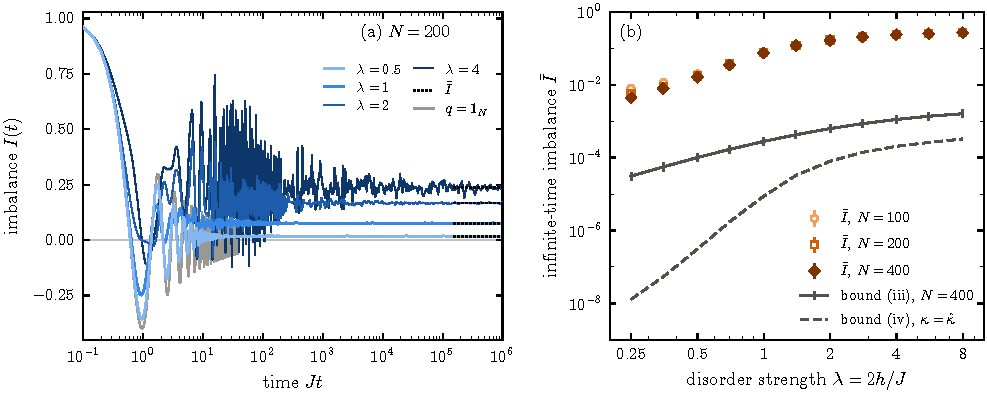
\includegraphics[width=\textwidth]{figs/imbalance.pdf}
\caption{Memory of the charge-density wave, for $\Psi_0=\ket{\uparrow\cdots\uparrow}_z\otimes\psicdw$ and $J=1$.
(a) Imbalance $I(t)$ for $N=200$ and $\lambda=2h/J=0.5,1,2,4$ (light to dark), averaged over the same $1000$
i.i.d.\ charge sectors at all times; uniform time grid for $Jt\le200$, logarithmic grid beyond.  The bands of
$\pm2$ standard errors are mostly thinner than the lines.  The short dotted segments at the right mark the
infinite-time average $\Ibar$ of \cref{thm:imbalance}(i), computed from the eigenvectors of the same sectors.
Grey: the clean sector $q=\one_N$ (for any $h$), shown for $Jt\le40$.  (b) $\Ibar$ versus $\lambda$ for
$N=100,200,400$ ($2000$ sectors each; the error bars of $\pm2$ standard errors are smaller than the symbols),
and the rigorous lower bounds of \cref{thm:imbalance} evaluated with the measured $\kappa_N$: the better of the two
bounds \eqref{eq:main-Ibound} at $N=400$ (solid), and the bound \eqref{eq:main-Iuniform} with $\kappa$ replaced by
$\kaphat=\max_N(\kappa_N+2\,\mathrm{SE})$ (dashed).  See \cref{tab:numerics-imbalance}.}
\label{fig:imbalance}
\end{figure}

\begin{table}[t]
\centering
\small
\setlength{\tabcolsep}{3pt}
\begin{tabular}{c|ccc|c|cc|cc}
$\lambda$ & $\Ibar_{100}$ & $\Ibar_{200}$ & $\Ibar_{400}$ & $\kappa_{400}$ & (iii), $N=400$ & (iv), $\kaphat$
 & $\Sigma_1(\Femp)$ & (iv), $2\Sigma_1(\Femp)$\\\hline
$0.25$ & $0.00782(10)$ & $0.00556(5)$ & $0.00433(3)$ & $43.22(3)$ & $3.1\times10^{-5}$ & $1.3\times10^{-8}$ & -- & --\\
$0.5$ & $0.01968(14)$ & $0.01732(9)$ & $0.01596(6)$ & $15.84(3)$ & $1.0\times10^{-4}$ & $3.1\times10^{-7}$ & -- & --\\
$1$ & $0.0788(4)$ & $0.0759(3)$ & $0.0745(2)$ & $4.95(2)$ & $2.8\times10^{-4}$ & $8.7\times10^{-6}$ & $104$ & $5.0\times10^{-9}$\\
$2$ & $0.1710(8)$ & $0.1672(5)$ & $0.1654(4)$ & $2.42(3)$ & $6.3\times10^{-4}$ & $7.9\times10^{-5}$ & $18.9$ & $3.4\times10^{-7}$\\
$4$ & $0.2402(11)$ & $0.2369(8)$ & $0.2362(5)$ & $2.02(2)$ & $1.1\times10^{-3}$ & $2.0\times10^{-4}$ & $10.9$ & $1.8\times10^{-6}$\\
$8$ & $0.2697(12)$ & $0.2669(9)$ & $0.2640(6)$ & $1.90(3)$ & $1.6\times10^{-3}$ & $3.3\times10^{-4}$ & $8.3$ & $4.5\times10^{-6}$
\end{tabular}
\caption{Infinite-time imbalance and the lower bounds of \cref{thm:imbalance} ($J=1$; $2000$ sectors for each
$N$ and $\lambda$).  $\Ibar_N$: measured $\Ibar$.  $\kappa_{400}$: measured $\kappa_N$ of \eqref{eq:main-kappa} at $N=400$.
(iii): the larger of the two bounds \eqref{eq:main-Ibound} at $N=400$, with $\kappa_N$ replaced by
$\kappa_N+2\,\mathrm{SE}$; at this $N$ it is always the global bound $h^2/(N(J+|h|)^2)$.  (iv), $\kaphat$: the right
side of \eqref{eq:main-Iuniform} with $\kappa=\kaphat=\max_{N\in\{100,200,400\}}(\kappa_N+2\,\mathrm{SE})$, which exceeds
$\kappa_{400}$ by at most $0.07$.  The proof
of \cref{thm:imbalance}(iv) uses $\kappa$ only through $\kappa_N\le\kappa$, so this number is a lower bound on $\Ibar$
for each of the three values of $N$; it is not a statement uniform in $N$.  Last two columns:
$\Sigma_1(\Femp)$ for the empirical correlator envelope $\Femp(d)=\max_x\E_qQ^{[1,400]}_q(x,x+d)$, made
non-increasing, and the right side of \eqref{eq:main-Iuniform} with the constant $\kappa=2\Sigma_1(\Femp)$ that the
proof of \cref{thm:imbalance}(iv) uses.  These are omitted for $\lambda\le0.5$, where $\Femp$ has not decayed at
$d=N-1$.}
\label{tab:numerics-imbalance}
\end{table}

\paragraph{Time traces.}  \Cref{fig:imbalance}(a) shows, in our conventions, the observable studied numerically
in \cite{SKKM2017}.  After a transient, the sector-averaged imbalance settles at a positive value.  This value
agrees with the infinite-time average $\Ibar$ computed from the eigenvectors: at $Jt=10^6$ we find
$I=0.0174(7)$, $0.0747(9)$, $0.1694(16)$ and $0.2365(20)$ for $\lambda=0.5,1,2,4$, against $\Ibar=0.0173(1)$,
$0.0760(4)$, $0.1668(8)$ and $0.2376(11)$ from the same sectors.  The clean sector $q=\one_N$, the only sector of
the strictly gauge-invariant subspace $G_j\equiv1$ (\cref{rem:gaussproj}), has no memory.  In infinite volume its
imbalance is $\sum_{m\in\Z}(-1)^mJ_m(2Jt)^2=J_0(4Jt)$, by Neumann's addition theorem for Bessel functions.  For
$N=200$ it differs from $J_0(4Jt)$ by less than $5\times10^{-3}$ for $Jt\le40$, and its time average vanishes
exactly (\cref{rem:gaussproj}(ii)).  The memory is produced by the sector average, through the mechanism in the
proof of \cref{thm:imbalance}(iii).

\begin{remark}[Slow, oscillatory relaxation at strong coupling; heuristic]\label{rem:num-oscillations}
For $\lambda\ge2$ the approach of $I(t)$ to $\Ibar$ is slow and oscillatory, with deviations far larger than the
statistical errors.  At $\lambda=4$, $I(t)$ oscillates between $-0.12$ and $0.75$ for $Jt\in[10,100]$, and
$I=0.134(2)$ at $Jt=100$ and $0.336(2)$ at $Jt=2.2\times10^3$.  For $Jt\in[10^4,10^6]$ it still deviates from
$\Ibar=0.2376(11)$ by up to $0.06$ ($26$ standard errors).  At $\lambda=2$ the deviations stay below $0.007$
($4$ standard errors) for $Jt\ge10^4$.  For $\lambda\le1$ the data for $Jt\ge10^3$ agree with $\Ibar$ to within
$2.7$ standard errors.

We attribute the slow oscillations to the binary nature of the disorder.  Consider two equal charges at odd
distance $k$, separated by $k-1$ opposite charges.  Their sites are resonant, and the particle that the CDW places
on one of them tunnels to the other through an effective hopping of order $J(2\lambda)^{-(k-1)}$.  This hopping
depends only on the local charge pattern, which takes finitely many values.  The resulting oscillations, at
frequencies $\omega_k\approx2J(2\lambda)^{-(k-1)}$, are therefore coherent across sectors and dephase only through
higher-order, environment-dependent corrections.  For $k=1$ (adjacent equal charges), $\omega_1\approx2J$ gives the
fast oscillations at early times.  Consistently, at $\lambda=4$ ($N=200$, $400$ sectors) the spectral weight of
$I_q(t)-\Ibar_q$ has sharp peaks at $\omega\approx0.030J$, $4.5\times10^{-4}J$ and $6.8\times10^{-6}J$, close to
$\omega_3$, $\omega_5$, $\omega_7=0.031J$, $4.9\times10^{-4}J$, $7.6\times10^{-6}J$.  These correspond to periods of
about $2\times10^2$, $1.3\times10^4$ and $8\times10^5$ in units of $1/J$.  The windows within a factor $1.2$ of $\omega_3$
and $\omega_5$ carry about half of the weight of their decades ($0.022$ of $0.047$, and $0.0029$ of $0.0061$;
\texttt{code/numerics\_imbalance\_spectral.out}).  This explanation is heuristic.  None of it affects $\Ibar$,
which is what \cref{thm:imbalance} controls.
\end{remark}

\paragraph{Infinite-time imbalance.}  \Cref{fig:imbalance}(b) and \cref{tab:numerics-imbalance} show that $\Ibar>0$
at every $\lambda$ considered, down to $\lambda=0.25$, and that $\Ibar$ increases with $\lambda$.  For $\lambda\ge1$ it
decreases by $2$--$6\%$ from $N=100$ to $N=400$.  A boundary correction describes this well: a fit
$\Ibar_N=\Ibar_\infty+c/N$ to the three values has $\chi^2\le2.2$ (one degree of freedom) and $c$ between $0.5$ and
$1.1$ for every $\lambda\ge1$; at $\lambda=2$, for instance, $\Ibar_\infty=0.1635(6)$.  For $\lambda\le0.5$ the convergence in $N$ is slow, as expected when the localization
length is comparable with $N$: $\Ibar=0.01968(14)$, $0.01732(9)$, $0.01596(6)$ at $\lambda=0.5$, and
$0.00782(10)$, $0.00556(5)$, $0.00433(3)$ at $\lambda=0.25$, for $N=100,200,400$.  \Cref{thm:imbalance}(iv) asserts a
positive lower bound uniform in $N$ for every $\lambda\neq0$.  At $\lambda\le0.5$ the data are compatible with it but
cannot test the uniformity: they only show that $\Ibar$ is positive and not yet converged at $N=400$.

\paragraph{The rigorous bounds.}  For $\lambda\ge1$ the measured $\kappa_N$ is nearly independent of $N$; for example
it is $4.83(1)$, $4.93(2)$, $4.95(2)$ at $\lambda=1$ and $2.37(1)$, $2.41(3)$, $2.42(3)$ at $\lambda=2$, for
$N=100,200,400$.  This agrees with the bound $\kappa_N\le\kappa$ of \cref{thm:imbalance}(iv).  For $\lambda\le0.5$ it still
grows with $N$ ($11.25(2)$, $14.27(3)$, $15.84(3)$ at $\lambda=0.5$).  All bounds lie below the data, as they must,
but by large factors.
\begin{itemize}
\item At $N=400$ the better of the bounds \eqref{eq:main-Ibound} is the global one, $h^2/(N(J+|h|)^2)$, which is
$140$--$280$ times smaller than $\Ibar$.  The block bound does not decay with $N$, but its optimal block length
$L\approx32\kappa_N^2$ exceeds $400$ for $\lambda\le1$.
\item The bound \eqref{eq:main-Iuniform}, evaluated with the measured $\kaphat$, is smaller than $\Ibar$ by factors
from $8\times10^2$ (at $\lambda=8$) to $3\times10^5$ (at $\lambda=0.25$).
\item With the constant $\kappa=2\Sigma_1(F)$ that the proof of \cref{thm:imbalance}(iv) uses, evaluated with the
empirical envelope $\Femp$, the bound drops by a further factor between $70$ (at $\lambda=8$) and $1.7\times10^3$
(at $\lambda=1$).
\end{itemize}
The losses have three sources.  The Cauchy--Schwarz step (Step~2 in the proof of \cref{thm:imbalance}) bounds
$\sum_\alpha a_\alpha^2m_\alpha(B)$ below by $X_B^2$ divided by $\sum_\alpha E_\alpha^2m_\alpha(B)\le4L(J+|h|)^2$, which is far
from equality.  In the anticoncentration step (Step~4), Szarek's constant $\sqrt{L/2}$ has to beat the leakage
$2\kappa_N$; this requires $L>8\kappa_N^2$, and the optimal $L$ is of order $32\kappa_N^2$.  Finally, $\kappa_N\le2\Sigma_1(F)$ replaces the time-averaged
probabilities $R_q$ by the correlator $Q_q$ and its envelope.  The content of \cref{thm:imbalance} is qualitative:
a positive memory, uniformly in $N$, for every $h\neq0$.  This is what the data show.

% ----------------------------------------------------------------------------
\subsection{Entanglement and number entropy}\label{sec:numerics:entropies}

\begin{figure}[t]
\centering
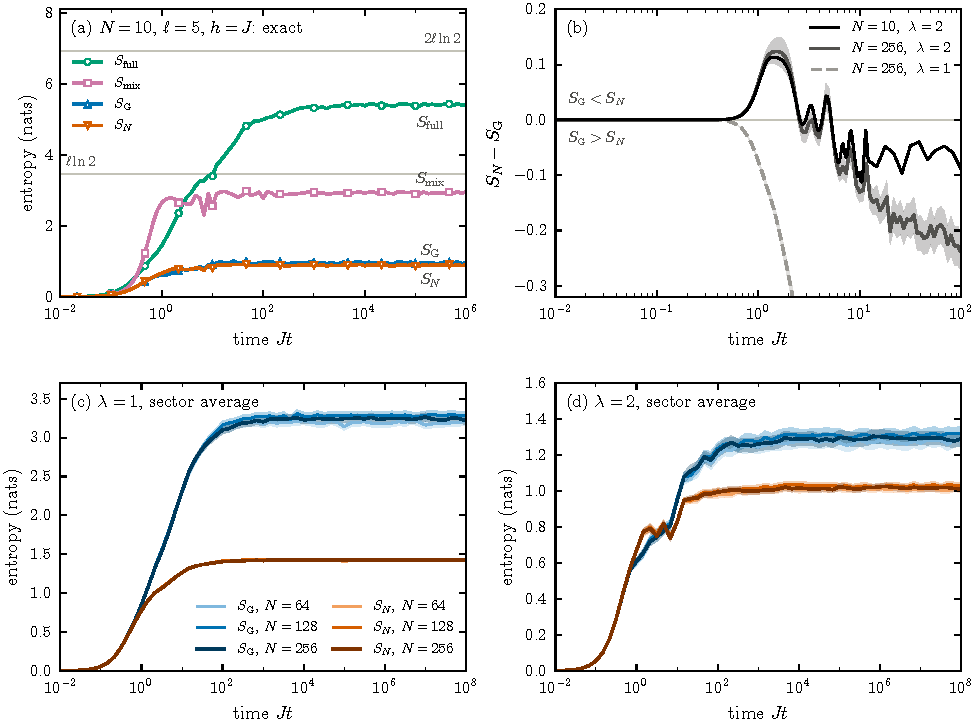
\includegraphics[width=\textwidth]{figs/entropies.pdf}
\caption{Entropies of the half chain after the quench from $\ket{\uparrow\cdots\uparrow}_z\otimes\psicdw$, $J=1$.
(a) Exact values for $N=10$, $\ell=5$, $h=J$ ($\lambda=2$), from the many-body state of the gauge theory (all $1024$
sectors, no sampling): the matter-plus-gauge entanglement $\Sfull$, the mixed dressed-matter entropy $\Smix$, the
conditional entanglement $\SG$ and the number entropy $\SN$.  Grey lines: the maxima $2\ell\ln2$ of $\Sfull$ and
$\ell\ln2$ of $\Smix$.  (b) $\SN-\SG$ at early times, for $N=10$ (exact; black) and for $N=256$ at $\lambda=2$ (dark grey) and $\lambda=1$
(grey, dashed), with $400$ sectors on a grid of $30$ times per decade and bands of $\pm2$ standard errors.  Positive values are counterexamples to the
inequality $\SG\ge\SN$ (\cref{rem:main-SGSN}).  (c), (d) The sector-averaged $\SG(t)$ (blue) and the number entropy
$\SN(t)$ of the mixture (vermillion), for $N=64,128,256$ (light to dark; $1000$ sectors each, bands of $\pm2$
standard errors), up to $Jt=10^8$, at $\lambda=1$ and $\lambda=2$.}
\label{fig:entropies}
\end{figure}

\paragraph{Exact data for $N=10$.}  \Cref{fig:entropies}(a) extends the table of \cref{rem:main-SGSN} to a dense
time grid ($97$ times in $[10^{-2},10^6]$).  The conditional entanglement $\SG$ is $0.91$ at $Jt=10$, and for
$Jt\in[10^3,10^6]$ it stays in $[0.93,0.99]$.  The full entanglement keeps growing over several decades, from
$\Sfull=1.45$ at $Jt=1$ to $3.40$, $5.00$ and $5.38$ at $Jt=10$, $10^2$ and $10^5$.  For $Jt\in[10^3,10^6]$ it stays in
$[5.30,5.45]$, below the maximum $2\ell\ln2=6.93$.  This is consistent with the logarithmic growth of
Conjecture~\ref{conj:logent} followed by finite-size saturation, but $N=10$ cannot separate the two.  The mixed
entropies saturate near $0.85\,\ell\ln2$: for $Jt\ge10^3$, $\Smix\in[2.89,2.97]$ and $\Sfm\in[2.92,3.00]$
(cf.\ Conjecture~\ref{conj:volmix}).  The number entropy stays in $[0.87,0.92]$.  The inequalities of
\cref{prop:entropies} hold at all $97$ times: $|\Sfull-S_{A'}(\Phi)|\le0.56<\ln2$, $\SG\le\Smix\le\ell\ln2$,
$\SN\le\min\{\Sfull,\Smix,\Sfm\}$ and $\E_q\Hsh(p^q_t)\le\min\{\SG,\SN\}$.

\paragraph{$\SG$ versus $\SN$.}  \Cref{fig:entropies}(b) shows where the false inequality $\SG\ge\SN$ fails.  For
$N=10$ (computed on a grid of step $0.005$ in $[0.05,12]$), $\SN-\SG>0$ for $0.05\le Jt<2.575$, with maximum $0.113$ at
$Jt\approx1.4$.  The difference then changes sign five times, at $Jt\approx2.58$, $2.93$, $3.63$, $4.25$ and $5.23$,
staying below $0.044$ in modulus, and $\SG>\SN$ at all later grid times up to $Jt=10^6$.  The same happens in large systems at $\lambda=2$.  For $N=256$
($400$ sectors, $30$ times per decade), $\SN-\SG$ exceeds two standard errors at all grid times
$0.015\le Jt\le2.33$, with maximum $0.124(11)$ at $Jt\approx1.5$.  On our grid it changes sign five times between
$Jt\approx2.5$ and $Jt\approx5.4$, staying below $0.044$ in modulus, and it is below minus two standard errors at all grid times
$5.4\le Jt\le10^2$.  At $\lambda=1$ (again $N=256$) the difference never exceeds
$2\times10^{-10}$, and it is below minus two standard errors for $Jt\ge0.074$.  Heuristically, the mechanism is the
one described in \cref{rem:main-SGSN}.  At early times about one particle crosses the cut, each $\rho^q_A$ is close to
a mixture of two number sectors, and so $\SG\approx\E_q\Hsh(p^q_t)\le\Hsh(\E_qp^q_t)=\SN$, by concavity.  The gap $\Hsh(\E_qp^q_t)-\E_q\Hsh(p^q_t)$ is the mutual information between $N_A$ and the charges, and it
grows with the spread of the per-sector laws.  At $Jt=1$ and $N=256$, the variance of the sector means
$\langle N_A\rangle_q$ (that is, $\Var_{p_t}(N_A)-\E_q\Var_q(N_A)$) is $0.039$ at $\lambda=2$ and $0.0053$ at $\lambda=1$; two
independent samples of $1000$ and $400$ sectors agree on these values to $3\%$.

\paragraph{Large $N$.}  \Cref{fig:entropies}(c), (d) show $\SG$ and $\SN$ for $N=64,128,256$ up to $Jt=10^8$.  Both
saturate after $Jt\approx10^2$--$10^3$.  They then stay flat: for every $N$ and both values of $\lambda$, the averages over
the grid times in $[10^3,10^5]$ and in $[10^6,10^8]$ differ by less than $0.01$, which is within the errors.  There is
no sign of the slow growth seen in $\Sfull$.  Averaging over the grid times $Jt\ge10^3$, with errors over sectors,
we find for $N=64,128,256$:
\begin{center}
\begin{tabular}{c|ccc|ccc}
 & \multicolumn{3}{c|}{$\SG$} & \multicolumn{3}{c}{$\SN$}\\
 & $N=64$ & $N=128$ & $N=256$ & $N=64$ & $N=128$ & $N=256$\\\hline
$\lambda=1$ & $3.19(2)$ & $3.28(2)$ & $3.24(2)$ & $1.420(4)$ & $1.431(4)$ & $1.425(4)$\\
$\lambda=2$ & $1.27(2)$ & $1.31(2)$ & $1.29(2)$ & $1.011(7)$ & $1.028(7)$ & $1.016(8)$
\end{tabular}
\end{center}
The values for different $N$ agree to within $3\%$.  The largest difference, $2.9$ standard errors, is between $N=64$
and $N=128$ for $\SG$ at $\lambda=1$, and the value for $N=256$ lies between the two.  This is what
\cref{thm:arealaw}(b) and \cref{thm:numberentropy} assert: both entropies are bounded uniformly in $t$ and $N$.  The
quantity bounded in \cref{thm:arealaw}(b) is $\E_q\sup_tS(\rho^q_A(t))$.  Its lower estimate
$\E_q\max_{t\in\mathcal T}S(\rho^q_A(t))$ over our time grid $\mathcal T$ is $3.92(3)$, $4.02(3)$, $3.96(3)$ at
$\lambda=1$ and $1.68(2)$, $1.74(2)$, $1.71(2)$ at $\lambda=2$, for $N=64,128,256$.

\paragraph{Size of the constants.}  The theorems hold with the true function $F$ of Hypothesis~\ref{hyp:EC}, whose
constants are not explicit (\cref{rem:rate}).  To indicate their size we insert the empirical envelope $\Femp$ of
\cref{tab:numerics-imbalance} ($N=400$).  At $\lambda=2$ this gives $2\ln2\,\Theta(\Femp)\approx1.3\times10^3$ for the
area-law bound of \cref{thm:arealaw}(b), against a measured $\E_q\max_{t\in\mathcal T}S(\rho^q_A(t))\approx1.7$.  It gives
$\frac12\ln(2\pi e(K_1+K_2+\frac1{12}))\approx6.3$ for the bound \eqref{eq:main-SN}, against a measured $\SN\approx1.0$.
At $\lambda=1$ the two bounds are $1.5\times10^4$ and $7.8$, against $4.0$ and $1.4$.  The number-entropy bound is much
closer to the data only because the constants enter it through a logarithm.  Inserting the \emph{measured} variance of
$N_A$ into \cref{lem:intentropy} gives $1.11$--$1.13$ at $\lambda=2$ and $1.47$--$1.48$ at $\lambda=1$ (maximum over $t$),
close to the measured $\SN$.  This uses the measured variance instead of the bound $K_1+K_2$, so it is not a consequence
of \cref{thm:numberentropy} (\cref{rem:main-numberentropy}).

% ----------------------------------------------------------------------------
\subsection{One-body localization and the dimer law}\label{sec:numerics:other}

Two further figures appear in the sections they illustrate.

\Cref{fig:correlator} (\cref{sec:onebody}) shows the annealed eigenfunction correlator $\E_qQ^{[1,N]}_q(x,x+d)$, the
quantity of Hypothesis~\ref{hyp:EC}, for boundary pairs ($x=1$) and bulk pairs ($x=N/2$) and $N=100,200,400$.  The
boundary and bulk correlators decay at the same rate and do not depend on $N$.  This is the content of
\cref{thm:EC}: uniformity in $N$ and in the position of the pair, including pairs at the fixed left end of the chain.
The fitted annealed rates reported in \cref{rem:onebodynumerics} lie well below the smallest Lyapunov exponent,
increasingly so as $\lambda$ grows, in line with \cref{rem:rate}(ii).

\Cref{fig:dimer} (\cref{sec:dimer}) shows one dressed fermion in a dimer product state, for which the sector law is the
random dimer law (\cref{prop:dimerlaw}).  At $h=0.25J$, where $0<2h<J$ and the dimer model has critical energies, the
sector-averaged mean-square displacement grows superdiffusively, roughly like $t^{3/2}$.  The time-averaged moment
$\Mom_2(T)$ of every sampled sector is bounded below by a multiple of $JT$, as \cref{prop:dimerlower} and
\cref{thm:dimer} assert.  For the i.i.d.\ law at the same $h$, and for the dimer law at $h=0.75J$, the mean-square displacement
saturates (\cref{rem:dimernumerics}).  The Hamiltonian is the same in all these runs; only the initial state differs, and with
it the sector law.  Together with \cref{fig:imbalance}, this illustrates that disorder-free localization is a
property of the sector law induced by the initial state (\cref{rem:dimermessage}).

% ----------------------------------------------------------------------------
\subsection{What the numerics do and do not show}\label{sec:numerics:summary}

\begin{remark}[Scope]\label{rem:num-scope}
(i) All data are for finite $N$ and finite times, and the sector averages for $N\ge64$ are Monte Carlo estimates
with the quoted errors.  They illustrate the theorems.  They cannot confirm statements about $N\to\infty$ or
$t\to\infty$, and they are not used in any proof.

(ii) Every rigorous bound that we evaluated holds in the data, and none is close to sharp.  With the measured
$\kappa_N$, the lower bounds on $\Ibar$ are $10^2$ to $3\times10^5$ times too small, and up to $1.5\times10^7$ times with
the constant of \cref{thm:imbalance}(iv) evaluated with $\Femp$.  Evaluated with $\Femp$, the area-law bound exceeds the
measured $\E_q\max_{t\in\mathcal T}S(\rho^q_A(t))$ by factors of about $8\times10^2$ ($\lambda=2$) and $4\times10^3$
($\lambda=1$), and the number-entropy bound exceeds the measured $\SN$ by factors of $5$--$6$.

(iii) The exact $N=10$ data are consistent with Conjectures~\ref{conj:logent} and~\ref{conj:volmix}, but they do
not test them.  A test would need the full many-body state of much larger systems.
\end{remark}

\section{Discussion and open problems}\label{sec:discussion}
Stub.


\appendix
% Long Lean identifiers cannot be hyphenated; set the appendix ragged right.
\begingroup
\raggedright
% ---------------------------------------------------------------------------
% Appendix: Formal verification in Lean
% ---------------------------------------------------------------------------
\section{Formal verification in Lean}\label{app:lean}

The finite-volume results of this paper are formalized in the proof assistant Lean~4 with the
Mathlib library (both at version 4.36.0), in the directory \texttt{lean/} of the repository that
accompanies the paper.  This appendix describes what the formalization contains, what it assumes,
and where it deviates from the text.

\paragraph{Objects.}  Everything is finite dimensional and defined from scratch:
\begin{itemize}
\item the Fock space of $N$ Jordan--Wigner fermions and the link spins, written in the $\sigma^x$
basis of the links;
\item the Hamiltonian~\eqref{eq:H}, the Gauss operators~\eqref{eq:gauss} and the boundary link, together
with the open chain, the ring, and the two-dimensional model on arbitrary finite graphs;
\item the dynamics, as matrix exponentials;
\item the eigenbases of the one-body operators, from Mathlib's spectral theorem;
\item the Shannon and von Neumann entropies.
\end{itemize}
Probabilities over the charges are uniform averages over $\{\pm1\}^N$.

\paragraph{Checking.}  The whole library compiles without \texttt{sorry}.  Every theorem listed below
depends only on Lean's three standard axioms (\texttt{propext}, \texttt{Classical.choice},
\texttt{Quot.sound}), as reported by \texttt{\#print axioms}.

\paragraph{The localization input.}  The theorems of \cref{sec:main} take Hypothesis~\ref{hyp:EC} as
an explicit argument (\texttt{EC J h F}).  In addition, the proof of \cref{thm:EC}(i) is formalized
(\texttt{ec\_of\_ldt}): Hypothesis~\ref{hyp:EC} follows from a hypothesis \texttt{LDT}.  This
hypothesis consists of two parts:
\begin{itemize}
\item the uniform large-deviation estimate \eqref{eq:LDTvec}, in vector form, for products of
i.i.d.\ Bernoulli transfer matrices;
\item a lower bound $\gamma_\lambda\ge\gamma_*>0$ on $\Ilam$.
\end{itemize}
Both are published theorems (\cref{prop:nocritical,prop:LDT}).  Their proofs, Furstenberg's theory
of products of random matrices, are not formalized.  The hypotheses of Furstenberg's theorem
(\cref{prop:nocritical}(i),(ii),(iv)) are formalized.  Consequently \cref{thm:transport},
\cref{thm:numberentropy}, \cref{thm:imbalance} and \cref{thm:arealaw}(a),(b) are Lean theorems whose
only external input is this literature result (\texttt{lgt\_transport\_of\_ldt},
\texttt{lgt\_numberEntropy\_of\_ldt}, \texttt{lgtImbalance\_lower\_of\_ldt}, \texttt{lgt\_areaLaw\_of\_ldt}).

\paragraph{Correspondence.}  Lean names, followed by their files:
\begin{itemize}[leftmargin=1.5em,itemsep=1pt]
\item \cref{thm:duality,lem:gauss,cor:sector}: \texttt{duality}, \texttt{gauss\_dual},
\texttt{numOp\_dual}, \texttt{sector\_average} (\texttt{Duality}, \texttt{Sector}).
\item \cref{lem:productlaw}: \texttt{sector\_average\_prod\_fock}, \texttt{sector\_average\_zprod}
(\texttt{ProductLaw}).
\item \cref{prop:variants}: \texttt{sector\_average\_open} (open chain); \texttt{ring\_duality},
\texttt{gaussRing\_dual\_zero}, \texttt{wilson\_dual}, \texttt{Hring\_ringVec},
\texttt{sector\_average\_ring} (ring) (\texttt{Variants}, \texttt{Ring}).
\item \cref{lem:pinching}, together with concavity and the mixing bound of the von Neumann entropy:
\texttt{vonNeumann\_le\_pinching}, \texttt{vonNeumann\_pinching\_le}, \texttt{vonNeumann\_concave},
\texttt{vonNeumann\_mix\_le} (\texttt{VNEntropy}).
\item \cref{lem:cutlocal}(b),(c),(d): \texttt{cutlocal\_defect}, \texttt{vonNeumann\_rdmLGT\_xprod},
\texttt{exProd\_U\_entropy}, \texttt{exProd\_Udag\_entropy} (\texttt{Entropies}, \texttt{CutLocal},
\texttt{CutLocalExamples}).
\item \cref{lem:consequences,hyp:EC}: \texttt{norm\_evo\_le\_corrQ}, \texttt{EC} (\texttt{OneBody}).
\item \cref{thm:EC}(i) with \cref{lem:green,lem:entry,lem:badset,lem:double}: \texttt{ec\_of\_ldt},
\texttt{poisson}, \texttt{box\_right}, \texttt{box\_left}, \texttt{entry\_ldt},
\texttt{exists\_resEnd}, \texttt{single\_box}, \texttt{two\_box} (\texttt{Transfer}, \texttt{Resonance},
\texttt{LDTEntry}, \texttt{ECProof}).
\item \cref{prop:nocritical}(i),(ii),(iv): \texttt{unipotent\_pow\_unbounded},
\texttt{no\_finite\_invariant\_lines}, \texttt{transferT\_commutator} (\texttt{Furstenberg}).
\item \cref{thm:transport}: \texttt{lgt\_transport}; \cref{prop:LR}: \texttt{avg\_norm\_comm\_le};
\cref{lem:duhamel}: \texttt{avg\_colNorm\_evo\_sub\_le} (\texttt{Main}, \texttt{LiebRobinson},
\texttt{Duhamel}).
\item \cref{thm:imbalance}: \texttt{lgtImbalance\_timeAvg}, \texttt{lgtImbalance\_lower}
(\texttt{Imbalance}, \texttt{Main}).
\item \cref{lem:intentropy,thm:numberentropy}: \texttt{massey}, \texttt{lgt\_numberEntropy}
(\texttt{Entropy}, \texttt{Main}).
\item \cref{thm:arealaw}: \texttt{lgt\_areaLaw}, \texttt{lgt\_areaLaw\_full} (\texttt{AreaLaw},
\texttt{CutLocal}).
\item \cref{prop:entropies}: (a) \texttt{lgt\_duality\_defect}; (b) \texttt{mixRdm\_eq\_marginal},
\texttt{condEntropy\_le\_mix}, \texttt{mix\_le\_cond\_add}, \texttt{mix\_le\_log},
\texttt{sectorLawEntropy\_le}, \texttt{sectorLawEntropy\_zero}; (c) \texttt{lgtNumDist\_eq\_avg},
\texttt{fullEntropy\_eq\_numberEntropy\_add}, \texttt{bareEntropy\_eq\_numberEntropy\_add},
\texttt{lgt\_numberEntropy\_le\_full}, \texttt{numberEntropy\_le\_mix}, \texttt{numberEntropy\_le\_bare},
\texttt{avg\_sector\_shannon\_le\_cond}, \texttt{numberEntropy\_le\_avg\_add}; (d)
\texttt{correlator\_eq\_ensemble} (\texttt{Entropies}, \texttt{EntropyBlocks}, \texttt{Taxonomy},
\texttt{Ensemble}).
\item \cref{prop:dimerlaw,lem:dimercritical}, \cref{prop:dimerimbalance}(i),(ii):
\texttt{sector\_average\_dimer}, \texttt{jsbs\_condition}, \texttt{dimerImbalance\_timeAvg}
(\texttt{Dimer}, \texttt{DimerCritical}, \texttt{DimerImbalance}).
\item \cref{lem:2dgauge}, \cref{thm:2dmap}(a),(b), on arbitrary finite graphs:
\texttt{flux\_eq\_iff\_gauge}, \texttt{card\_gaugeOrbit}, \texttt{card\_fluxClasses},
\texttt{wilsonLoop\_comm\_ham}, \texttt{gaussOp\_prod}; the joint eigenvectors $V_{q,s}\ket n$:
\texttt{fluxVec\_gauss}, \texttt{fluxVec\_wilson}, \texttt{fluxVec\_gaugeAct},
\texttt{fluxVec\_orthogonal}, \texttt{card\_fluxLabels}, \texttt{ham\_fluxVec} (\texttt{GraphFlux},
\texttt{GraphWilson}, \texttt{TwoDMap}).
\item \cref{prop:2dlaws}: (a) \texttt{sector\_average\_flux} (and \texttt{sector\_average\_matter}
for $s=+$); (b) \texttt{sector\_average\_xpol}, \texttt{xpol\_summand\_gauge}; (c)(i),(ii)
\texttt{checkerboard\_sq}, \texttt{checkerboard\_gap}, \texttt{checkerboard\_edge\_iff}
(\texttt{Graph}, \texttt{GraphFlux}, \texttt{TwoD}).
\item \cref{prop:nocompact}: \texttt{no\_compact\_eigenvector} (\texttt{TwoD}).
\item \cref{prop:cluster}: \texttt{hqs0\_cluster}, \texttt{cluster\_bound}, \texttt{cluster\_leak},
\texttt{cluster\_avg} (\texttt{Cluster}).
\item \cref{prop:gausscap}: \texttt{countInt\_gauss}, \texttt{qlm\_numberEntropy\_le},
\texttt{qlm\_numberEntropy\_le\_super}, \texttt{qlm\_sector\_preserved}, \texttt{bgEntropy\_invariant}
(\texttt{QLM}, \texttt{QLMSuper}).
\item \cref{prop:wilson}: \texttt{wField\_eq\_count}, \texttt{wilson\_field\_bound},
\texttt{wilson\_numberEntropy\_avg}, \texttt{wilson\_numberEntropy\_most},
\texttt{wilson\_numberEntropy\_each} (\texttt{Wilson}).
\item \cref{rem:randomwalk}: \texttt{Hstd\_dual\_oneP}, \texttt{partialSum\_bijective}
(\texttt{RandomWalk}).
\end{itemize}

\paragraph{Deviations.}  Sites and links are indexed from $0$.  The constants of
\cref{thm:numberentropy}, \cref{thm:arealaw} and \cref{thm:EC} appear as existential quantifiers, with
values depending only on $J$, $h$ and the profile $F$ (resp.\ on $|\lambda|$).  The Lean area law
has the constant $2$ in place of $2\ln2$.  Three proofs take a different route from the text.
\begin{itemize}
\item \Cref{lem:green} is replaced by the Poisson identity
$\det(E-A_B)\,\varphi(x)=\det(E-A_{[x+1,b]})\,\varphi(a-1)+\det(E-A_{[a,x-1]})\,\varphi(b+1)$, valid
for every solution of the eigenvalue equation on $B=[a,b]$ (a Wronskian argument).
\item \Cref{lem:entry} uses only the vector form \eqref{eq:LDTvec} of the large-deviation estimate:
the norm of the product is bounded through its action on two basis vectors.
\item In \cref{prop:cluster}(b) the generator $S$ is obtained from the anticommutator equation
$\Gamma h^0S+S\Gamma h^0=\Gamma h^1$ with $\Gamma=\operatorname{sgn}(h)\diag(q)$, so that
$[h^0,S]=h^1$ and $\norm S\le\norm{h^1}/g$, using $\Gamma h^0\ge g/2$.  The mean value inequality
for $u\mapsto\e^{\ii uh}(\one-S)\e^{-\ii uh^0}$ then gives
$\norm{\e^{-\ii th}-\e^{-\ii th^0}}\le2\norm S+\abs t\norm{h^1}\norm S$, i.e.\ \eqref{eq:clusterbound}
with $16$ in place of $48$.
\end{itemize}

\paragraph{Not formalized.}  The following are not formalized:
\begin{itemize}
\item the literature results entering as inputs: the large-deviation estimate together with the
positivity and continuity of the Lyapunov exponent, \cref{prop:nocritical}(iii), \cref{prop:Zline},
the transport bounds of \cite{JSBS2003} behind \cref{thm:dimer}, and the percolation estimate of
\cite{LiL2022}, which enters \texttt{cluster\_avg} as the probability that the cluster leaves the
region;
\item the infinite-volume statements: \cref{thm:infvol}, \cref{cor:ECinfvol}, \cref{thm:EC}(ii) and
\cref{prop:dimerimbalance}(iii);
\item in two dimensions, \cref{thm:2dmap}(c),(d) (planar boxes and tori) and
\cref{prop:2dlaws}(c)(iii),(iv);
\item remarks, conjectures and numerics.
\end{itemize}

\par
\endgroup

\bibliographystyle{unsrt}
\bibliography{refs}
\end{document}
